% This must be in the first 5 lines to tell arXiv to use pdfLaTeX, which is strongly recommended.
\pdfoutput=1
% In particular, the hyperref package requires pdfLaTeX in order to break URLs across lines.

\documentclass[11pt]{article}

% Change "review" to "final" to generate the final (sometimes called camera-ready) version.
% Change to "preprint" to generate a non-anonymous version with page numbers.
\usepackage[final]{acl}
% \usepackage[preprint]{acl}

% Standard package includes
\usepackage{times}
\usepackage{latexsym}

% For proper rendering and hyphenation of words containing Latin characters (including in bib files)
\usepackage[T1]{fontenc}
% For Vietnamese characters
% \usepackage[T5]{fontenc}
% See https://www.latex-project.org/help/documentation/encguide.pdf for other character sets

% This assumes your files are encoded as UTF8
\usepackage[utf8]{inputenc}

% This is not strictly necessary, and may be commented out,
% but it will improve the layout of the manuscript,
% and will typically save some space.
\usepackage{microtype}

% This is also not strictly necessary, and may be commented out.
% However, it will improve the aesthetics of text in
% the typewriter font.
\usepackage{inconsolata}

%Including images in your LaTeX document requires adding
%additional package(s)
\usepackage{graphicx}
\usepackage{hyperref}       % hyperlinks
\usepackage{url}            % simple URL typesetting
\usepackage{booktabs}       % professional-quality tables
\usepackage{amsfonts}       % blackboard math symbols
\usepackage{nicefrac}       % compact symbols for 1/2, etc.
\usepackage{microtype}      % microtypography
\usepackage{xcolor}         % colors
\usepackage{multirow}
\usepackage{float}
\usepackage{amsmath}
\usepackage{subcaption}
\usepackage{wrapfig}
\usepackage[most]{tcolorbox}
\usepackage{enumitem}
\usepackage{stfloats}
\usepackage{tcolorbox}   % 支持 \newtcolorbox
\tcbuselibrary{skins}    % (可选) 支持 enhanced 等高级功能

\usepackage{colortbl}
\usepackage{xcolor}
\definecolor{mygreen1}{rgb}{0.9686, 0.9804, 0.9843}  % Lightest blue
\definecolor{mygreen2}{rgb}{0.7961, 0.8745, 0.9216}  % Lighter blue
\definecolor{mygreen3}{rgb}{0.6235, 0.7647, 0.8588}  % Medium blue
\definecolor{mygreen4}{rgb}{0.3686, 0.5961, 0.7608} % Darker blue

\usepackage{mathtools}
\usepackage{amsthm}
\theoremstyle{plain}
\newtheorem{findings}{Findings}
\newtheorem{type}{Type}
\renewcommand{\thetype}{\Roman{type}}
\newtheorem{desideratum}{Desideratum}
    
% If the title and author information does not fit in the area allocated, uncomment the following
%
%\setlength\titlebox{<dim>}
%
% and set <dim> to something 5cm or larger.

% \title{Learning to Cut Losses: Single Token for Adaptive Path Pruning in Large Reasoning Models}
% \title{Learning to Cut Losses: A Closer Look at Path Pruning for Efficient Parallel Reasoning}
\title{\textit{Cut Your Losses!} Learning to Prune Paths Early for Efficient Parallel Reasoning}


\author{
   Jiaxi Bi$^{1,3}$\thanks{~~Equal contribution; alphabetical by last name.}\thanks{~~Work done during interning at CUHK-Shenzhen.}
   \quad  Tongxu Luo$^{1,2*}$  
   \quad  Wenyu Du$^{4}$ 
   \quad  \textbf{Zhengyang Tang$^{1}$} 
   \quad \textbf{Benyou Wang$^{1,2}$\thanks{~~Corresponding author.}} \\
  $^{1}$The Chinese University of Hong Kong, Shenzhen \\
  $^{2}$Shenzhen Loop Area Institute \\
  $^{3}$USTB \quad
  $^{4}$DualityRL
  \\
  \texttt{jiaxibi@xs.ustb.edu.cn \quad tongxuluo@cuhk.edu.cn \quad wangbenyou@cuhk.edu.cn} 
}


\newcommand{\tx}[1]{[\textcolor{cyan}{tx: #1}]}

\begin{document}
\maketitle
\begin{abstract}
% Parallel reasoning techniques significantly enhance the accuracy of Large Reasoning Models (LRMs) but incur prohibitive computational costs due to the generation of futile paths, often stemming from early, irreversible errors. 
% While path pruning offers a promising remedy, its practical utility is currently impeded by three critical deficits: \textbf{(D1) the lack of a unified framework} for comprehensive evaluation; \textbf{(D2) unverified test-time scalability}; and \textbf{(D3) the absence of empirical guidelines} for deployment. 
% To address \textbf{D1}, we present \textbf{the first systematic investigation} into path pruning, categorizing existing signal generators ($S$) based on their \textit{source} (internal vs. external) and \textit{nature} (learnable vs. non-learnable). 
% This taxonomy reveals the unexplored potential of \textit{learnable internal modules} ($S_\text{module}$), motivating us to introduce \textbf{STOP}, the first efficient instantiation of this paradigm. 
% Extensive evaluations across four LRMs (1.5B to 20B) on five math and stem benchmarks demonstrate that $S_\text{module}$ outperforms all other paradigms in both effectiveness and efficiency. 
% Motivated by these promising results, we rigorously validate the scalability of these methods under varying computational budgets for \textbf{D2}. 
% Results show $S_\text{module}$ is scalable and consistently performs well.
% For example, GPT-OSS-20B with $S_\text{module}$ improves the accuracy from 84\% to nearly 90\% under 175k tokens resources.
% Finally, addressing \textbf{D3}, we distill our findings into a formalized guideline to determine the best retention ratio of $S_\text{module}$.
% Our in-depth analysis and ablations also provide insights for understanding $S_\text{module}$.
% Code is provided in the supplementary material.

% Parallel reasoning significantly enhances Large Reasoning Models (LRMs) but incurs prohibitive costs due to futile paths generated from early errors. 
% While path pruning offers a remedy, its utility is impeded by three deficits: \textbf{(D1) the lack of a unified evaluation framework}; \textbf{(D2) unverified test-time scalability}; and \textbf{(D3) the absence of deployment guidelines}. 
% To address \textbf{D1}, we propose a systematic taxonomy classifying pruning signals by their \textit{source} (internal vs. external) and \textit{nature} (learnable vs. non-learnable).
% This reveals the unexplored potential of \textit{learnable internal modules} ($S_\text{module}$), leading to our proposal of \textbf{STOP}. 
% Extensive evaluations across four LRMs (from 1.5B to 20B) on five benchmarks demonstrate that $S_\text{module}$ outperforms existing paradigms in both effectiveness and efficiency. 
% Regarding \textbf{D2}, we validate that STOP scales robustly; for instance, it boosts GPT-OSS-20B accuracy from 84\% to nearly 90\% under a fixed 175k token budget. 
% Finally, addressing \textbf{D3}, we distill our findings into a formalized guideline for determining optimal retention ratios and provide in-depth analysis of the mechanism. 
% Code is provided in the supplementary material.
% \end{abstract}

Parallel reasoning enhances Large Reasoning Models (LRMs) but incurs prohibitive costs due to futile paths caused by early errors. 
To mitigate this, path pruning at the prefix level is essential, yet existing research remains fragmented without a standardized framework. 
In this work, we propose the first systematic taxonomy of path pruning, categorizing methods by their signal \textit{source} (internal vs. external) and \textit{learnability} (learnable vs. non-learnable). 
This classification reveals the unexplored potential of \textit{learnable internal methods}, motivating our proposal of \textbf{STOP} (\textbf{S}uper \textbf{TO}ken for \textbf{P}runing). 
Extensive evaluations across LRMs ranging from 1.5B to 20B parameters demonstrate that STOP achieves superior effectiveness and efficiency compared to existing baselines. 
Furthermore, we rigorously validate the scalability of STOP under varying compute budgets—for instance, boosting GPT-OSS-20B accuracy on AIME25 from 84\% to nearly 90\% under fixed compute budgets. 
Finally, we distill our findings into formalized empirical guidelines to facilitate optimal real-world deployment. 
Code, data and models are available at \url{https://bijiaxihh.github.io/STOP}.
\end{abstract}

\section{Introduction}\label{sec:Introduction}
% The proliferation of Large Reasoning Models (LRMs)~\cite{openai2024a,openai2024b,openai2025o3,guo2025deepseek,qwq32b,openai2025gptoss,google2025gemini25pro,alibaba2025qwen3max,anthropic2024claude35,wen2025lightr1,skywork2025or1,deepseekai2025deepseekr1incentivizingreasoningcapability} has unlocked remarkable capabilities in complex problem-solving.
% Parallel reasoning~\cite{wang2025survey_parallel_reasoning}, which generates a huge amount of reasoning paths for one question, has become standard practice for pushing the boundaries of reasoning accuracy.

% However, these improvements inevitably introduce considerable computation, typically up to 64 even 128 for one problem~\cite{deepseekmath2024,deepseekai2025deepseekr1incentivizingreasoningcapability,kang2025selfcertainty}.
% % ~\tx{cite deepseek, or other paper use cons@64}.
% This process substantially increases energy consumption (up to $113\times$ according to~\citet{jin2025energy}) and can raise the cost to nearly \$6 per query~\cite{nvidia2025inferencecost}. 
% These observations naturally raise a fundamental question: \textbf{Is such extensive computation truly necessary?}

% Recent studies~\cite{luo2025peers,hassid2025short} reveal that a substantial fraction of this computational effort is squandered on unproductive reasoning paths.
% \textbf{Not every path contributes positively to the final answer}; many are flawed from their inception.
% This issue is exacerbated by phenomena like the ``Prefix Dominance Trap''~\cite{luo2025peers}, where an LRM, having made an early error, struggles to self-correct and remains committed to a futile trajectory.
% The consequence is twofold: not only are valuable computational resources wasted, but these erroneous paths can also poison the final aggregation process, actively degrading the model's accuracy.

% \begin{figure*}[ht]
% \vspace{-14mm}
%   \centering
%   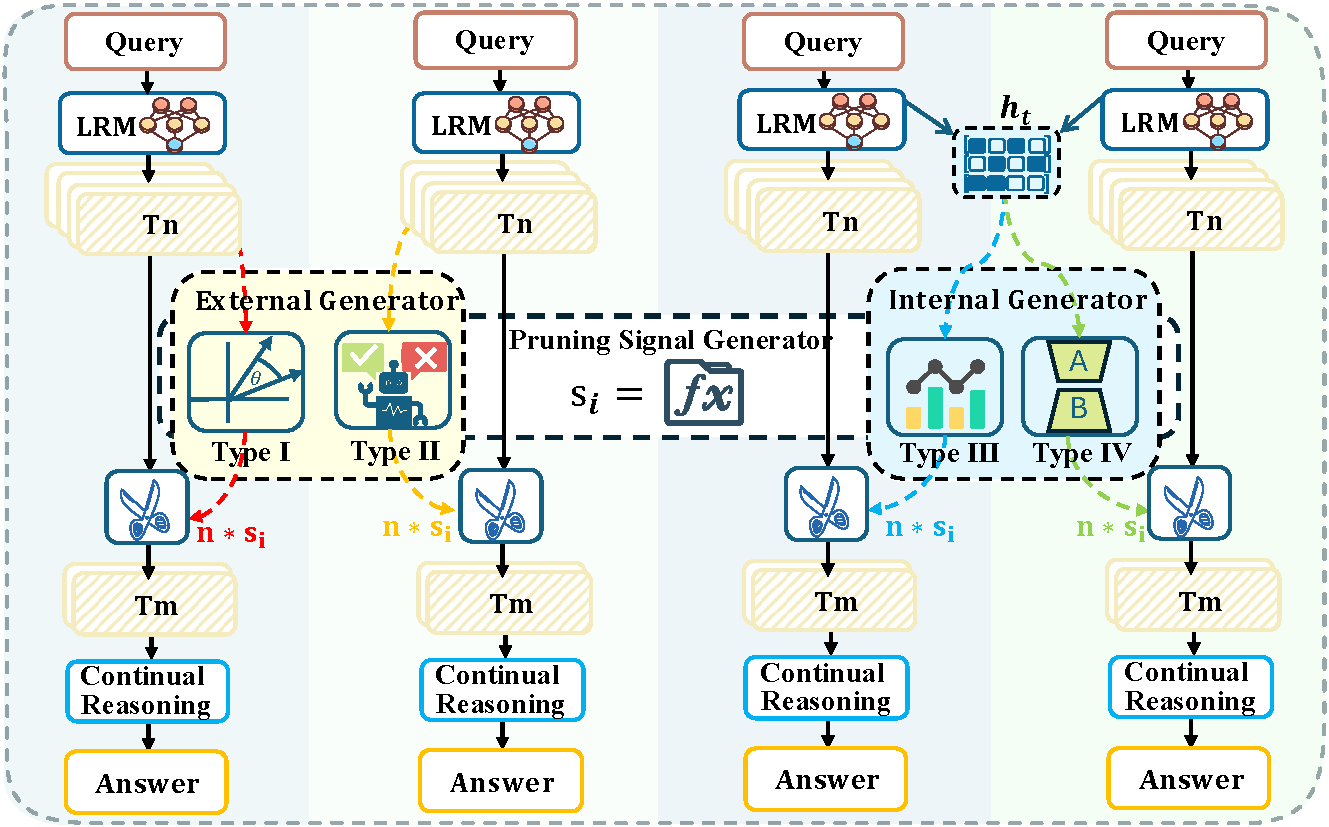
\includegraphics[width=0.9 \linewidth]{figures/main.pdf}
%   \caption{The proposed unified taxonomy of path pruning.}
%   \label{fig:main}
% \vspace{-4mm}
% \end{figure*}

% One promising research direction to mitigate these costs is path pruning, which terminates unpromising reasoning paths early to save computation and filter flawed logic. 
% Existing approaches generally rely on auxiliary models (e.g., Process Reward Models~\cite{liao2025lost,tu2025deepprune}), internal confidence signals~\cite{fu2025deepthink}, or semantic redundancy~\cite{hong2025slimsc}. 
% However, the practical utility of these methods is currently impeded by three critical deficits: 
% \textbf{(D1) the lack of a unified framework} to systematically compare diverse pruning signals; 
% \textbf{(D2) unverified scalability} across varying computational budgets; 
% and \textbf{(D3) the absence of empirical guidelines} for real-world deployment. 
% These gaps limit our understanding of the underlying trade-offs and hinder the optimal allocation of resources between exploration and exploitation.

% To address \textbf{D1}, we propose the first systematic taxonomy of path pruning, classifying methods based on the \textit{source} (external vs. internal) and \textit{nature} (learnable vs. non-learnable) of their signals. 
% This classification reveals that prior works occupy only three of the four quadrants, leaving the category of \textit{learnable internal modules} unexplored. 
% To bridge this gap, we introduce \textbf{STOP} (\textbf{S}uper \textbf{TO}ken for \textbf{P}runing), the first efficient instantiation of this paradigm. 
% Through comprehensive evaluation, we demonstrate that STOP achieves superior performance compared to existing baselines. 
% We further address \textbf{D2} by rigorously validating the scalability of our method across diverse model sizes and compute budgets, and resolve \textbf{D3} by deriving actionable empirical guidelines from our analysis to facilitate future research and deployment.

% In summary, this work makes four primary contributions:
% (1) we present the first systematic investigation and taxonomy of path pruning, identifying four types of pruning signal generators;
% (2) we propose STOP as the first method based on internal learnable signals;
% (3) we conduct a comprehensive evaluation on effectiveness and scalability of four pruning signal generators;
% (4) and we provide empirical guidelines to support practical implementation.

% \paragraph{The prohibitive cost of parallel reasoning.}
% The proliferation of Large Reasoning Models (LRMs) has established parallel reasoning as the standard for solving complex problems~\cite{openai2024a,wang2025survey_parallel_reasoning}.
% However, this accuracy gain comes at a prohibitive price.
% Generating dozens or even hundreds of reasoning paths per query increases energy consumption by orders of magnitude~\cite{jin2025energy} and escalates inference costs to nearly \$6 per query~\cite{nvidia2025inferencecost}.
% Crucially, recent studies reveal that this extensive computation is largely squandered: \textbf{not every path contributes to the solution}.
% Many trajectories are flawed from inception, yet they consume equal resources to generate and subsequently pollute the final answer aggregation~\cite{luo2025peers,hassid2025short}.

% \begin{figure}[h]
%     \centering
%     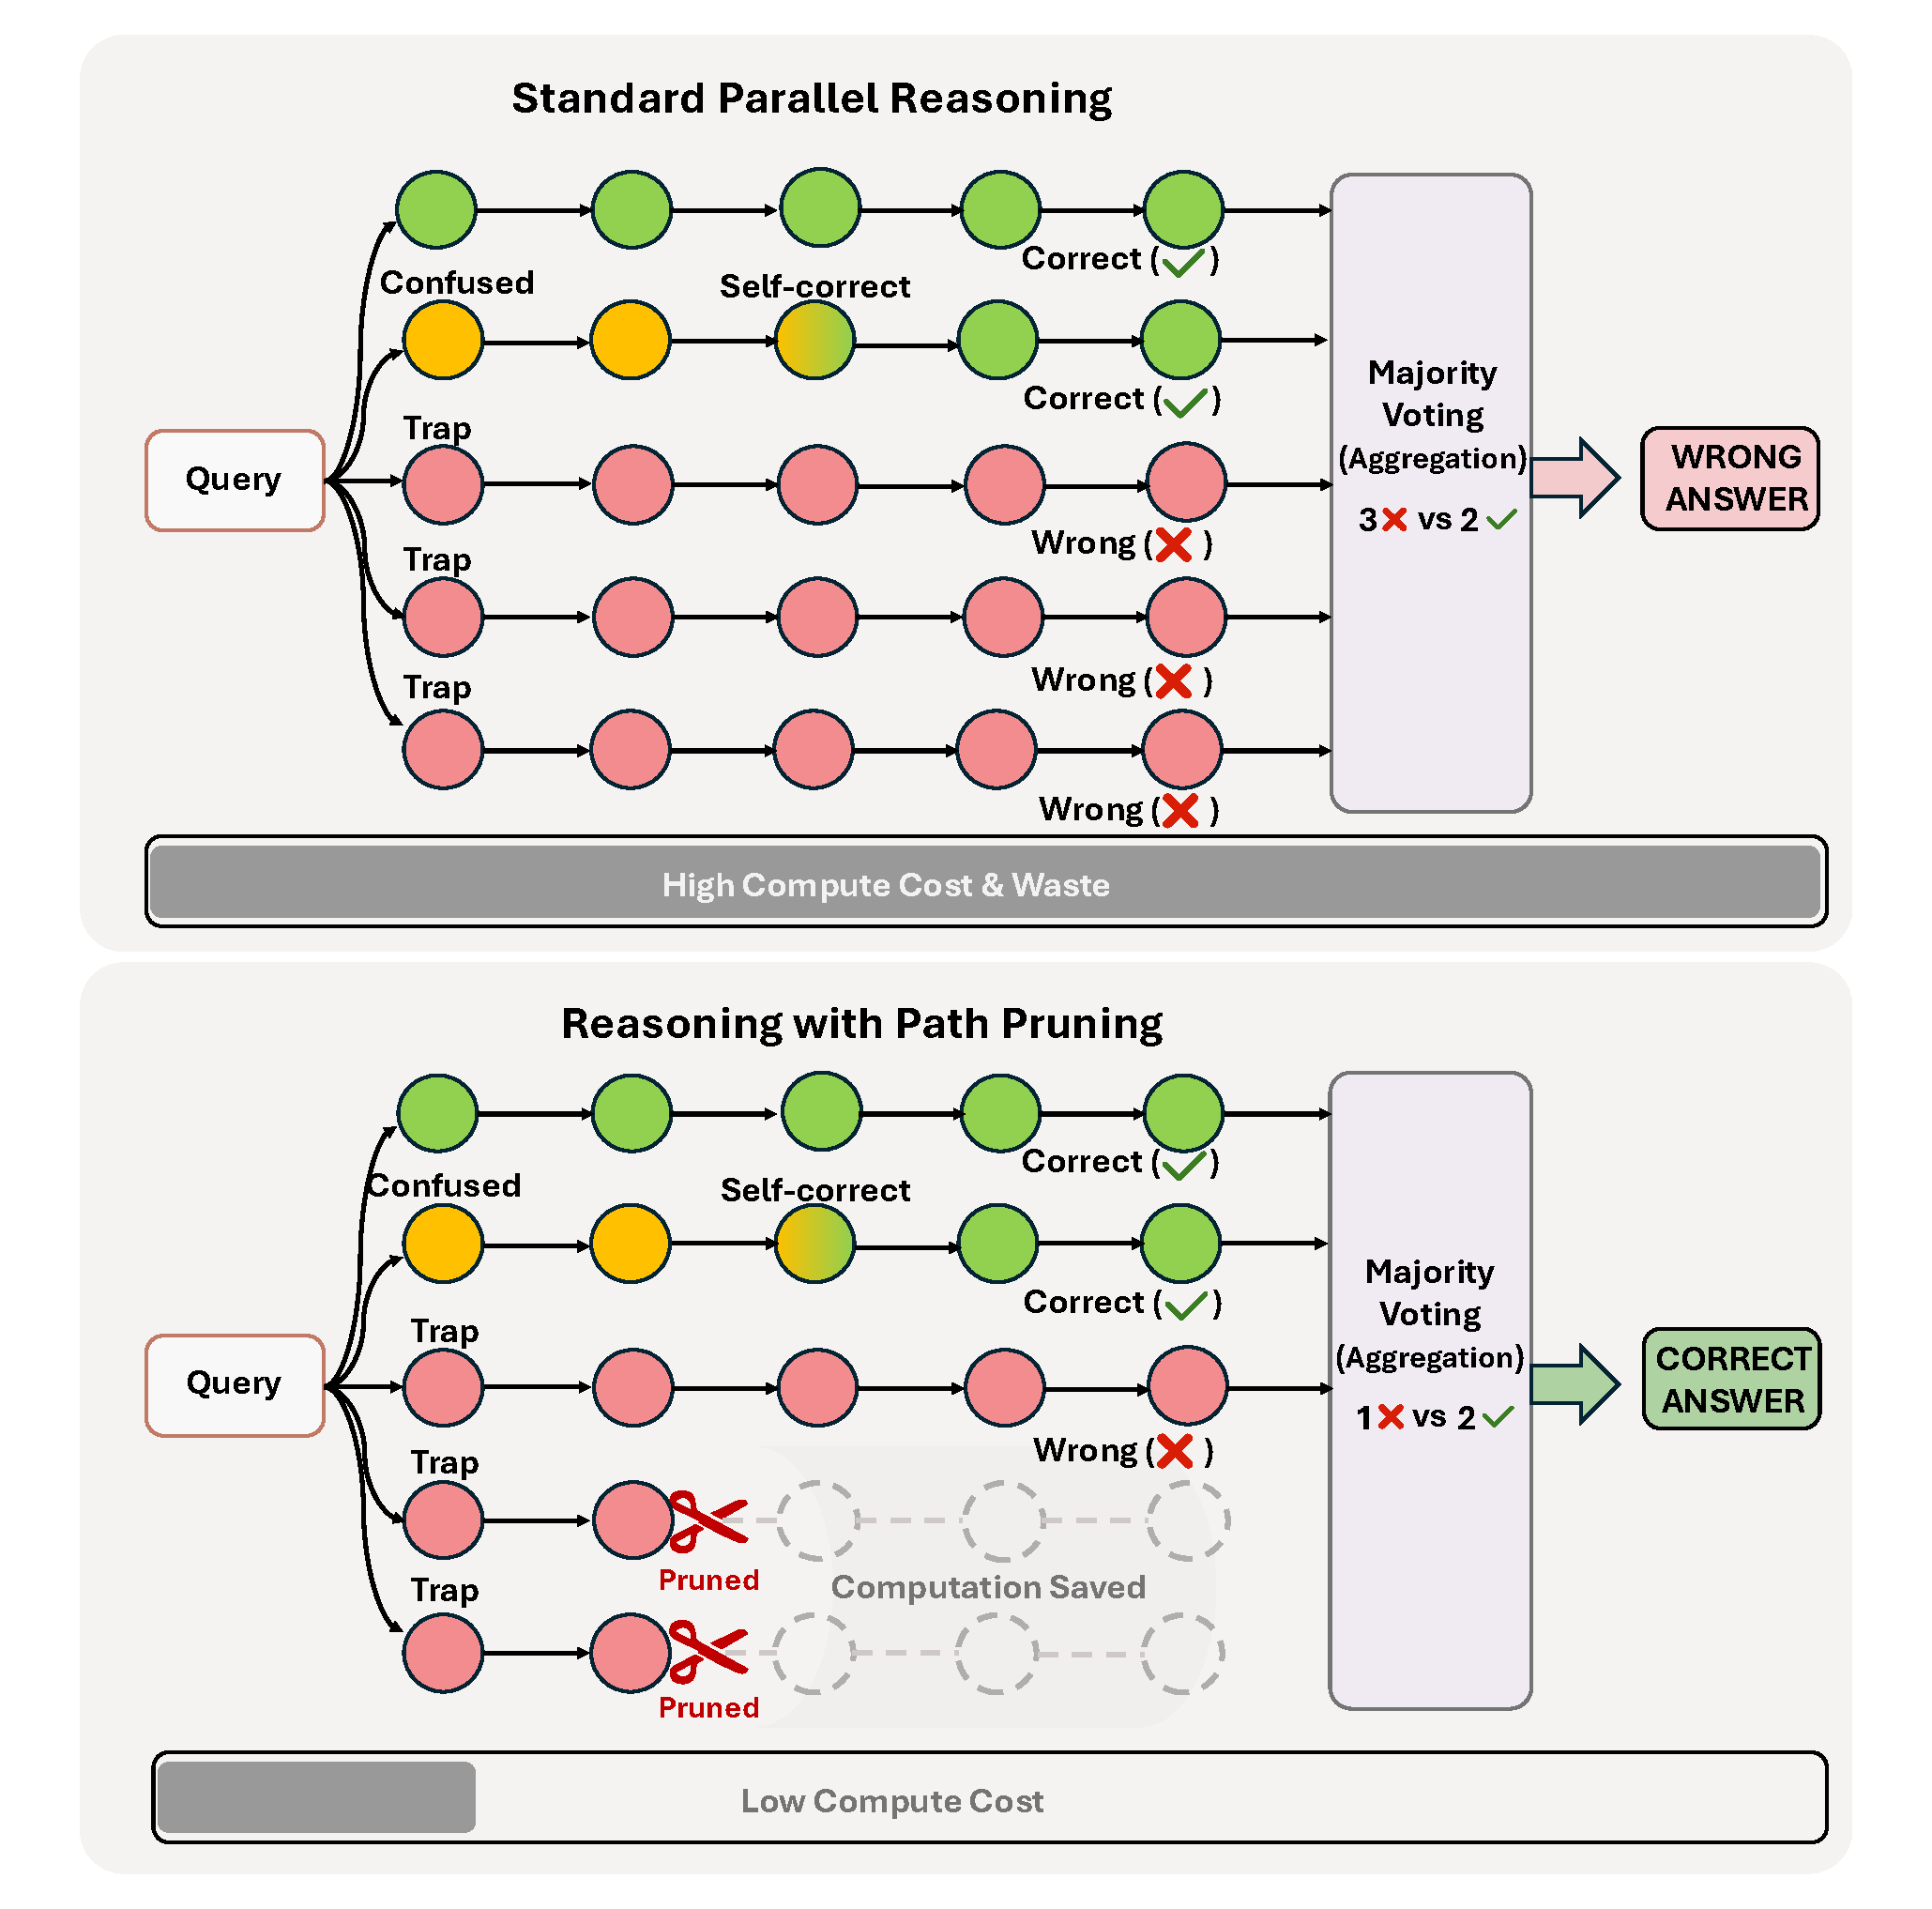
\includegraphics[width=\linewidth]{figures/motivation.pdf} 
%     % TODO: Replace with your motivation figure showing: 
%     % (Left) Bad prefix -> Full Rollout -> Waste & Error; 
%     % (Right) Bad prefix -> Pruned -> Compute saved for promising paths.
%     % \fbox{\rule{0pt}{2in} \rule{0.9\linewidth}{0pt} \textbf{[PLACEHOLDER: Motivation Figure]}}
%     \caption{The necessity of early pruning. Early errors in the reasoning prefix often lead to irreversible failure (the ``Prefix Dominance Trap''). Pruning these futile paths early not only saves computation but also purifies the candidate set for better consensus.}
%     \label{fig:motivation}
% \end{figure}

% \textbf{The prefix dominance trap.}
% This inefficiency stems from a phenomenon we term the ``Prefix Dominance Trap''~\cite{luo2025peers}.
% As illustrated in Figure~\ref{fig:motivation}, once a reasoning path begins with a flawed prefix, the LRM struggles to self-correct, inevitably spiraling into a futile trajectory.
% Consequently, identifying and terminating these unpromising paths at the \textit{prefix level}—a technique known as \textbf{path pruning}—is essential.
% While existing methods attempt to filter paths using auxiliary reward models~\cite{liao2025lost}, internal confidence~\cite{fu2025deepthink}, or semantic redundancy~\cite{hong2025slimsc}, their practical deployment is currently impeded by three critical deficits:
% \textbf{(D1) The lack of a unified framework} to systematically compare diverse pruning signals;
% \textbf{(D2) Unverified scalability} across varying computational budgets; and
% \textbf{(D3) The absence of empirical guidelines} for real-world deployment.

% To address \textbf{D1}, we propose the first systematic taxonomy of path pruning, classifying methods based on the \textit{source} (internal vs. external) and \textit{nature} (learnable vs. non-learnable) of their signals (Figure~\ref{fig:main}).
% This taxonomy reveals a significant gap: the unexplored potential of \textit{learnable internal modules}.
% To bridge this, we introduce \textbf{STOP} (\textbf{S}uper \textbf{TO}ken for \textbf{P}runing), the first efficient instantiation of this paradigm.
% Extensive evaluations demonstrate that STOP outperforms existing baselines in both effectiveness and efficiency.
% We further resolve \textbf{D2} by rigorously validating the scalability of STOP across diverse model sizes (1.5B to 20B) and compute budgets.
% Finally, for \textbf{D3}, we distill our analysis into actionable empirical guidelines to facilitate future research.

% In summary, our contributions are:
% (1) We present the first systematic investigation and taxonomy of path pruning.
% (2) We propose STOP, a novel pruning method based on learnable internal signals.
% (3) We provide a comprehensive evaluation demonstrating STOP's superior scalability and effectiveness.
% (4) We establish empirical guidelines to support the practical implementation of path pruning.

% \paragraph{The prohibitive cost of parallel reasoning.}


% Parallel Reasoning  is nice since ~~~;
Parallel reasoning has established itself as a standard paradigm for solving complex problems~\cite{openai2024a,wang2025survey_parallel_reasoning}.
The core principle is to sample multiple independent reasoning paths and subsequently aggregate them to derive a robust consensus.
However, this accuracy gain comes at a prohibitive cost.
Generating dozens or even hundreds of trajectories per query increases computational overhead by orders of magnitude~\cite{jin2025energy} and escalates inference costs to nearly \$6 per query~\cite{nvidia2025inferencecost}.

% The proliferation of Large Reasoning Models (LRMs) has established parallel reasoning as the standard for solving complex problems~\cite{openai2024a,wang2025survey_parallel_reasoning}.
% However, this accuracy gain comes at a steep price.
% Generating dozens or even hundreds of reasoning paths per query increases energy consumption by orders of magnitude~\cite{jin2025energy} and escalates inference costs to nearly \$6 per query~\cite{nvidia2025inferencecost}.
% Crucially, recent studies reveal that this extensive computation is largely squandered: \textbf{not every path contributes to the solution}.
% Many trajectories are flawed from inception, yet they consume equal resources to generate and subsequently pollute the final answer aggregation~\cite{luo2025peers,hassid2025short}.

\begin{figure}[t]
    \centering
    \vspace{-2mm}
    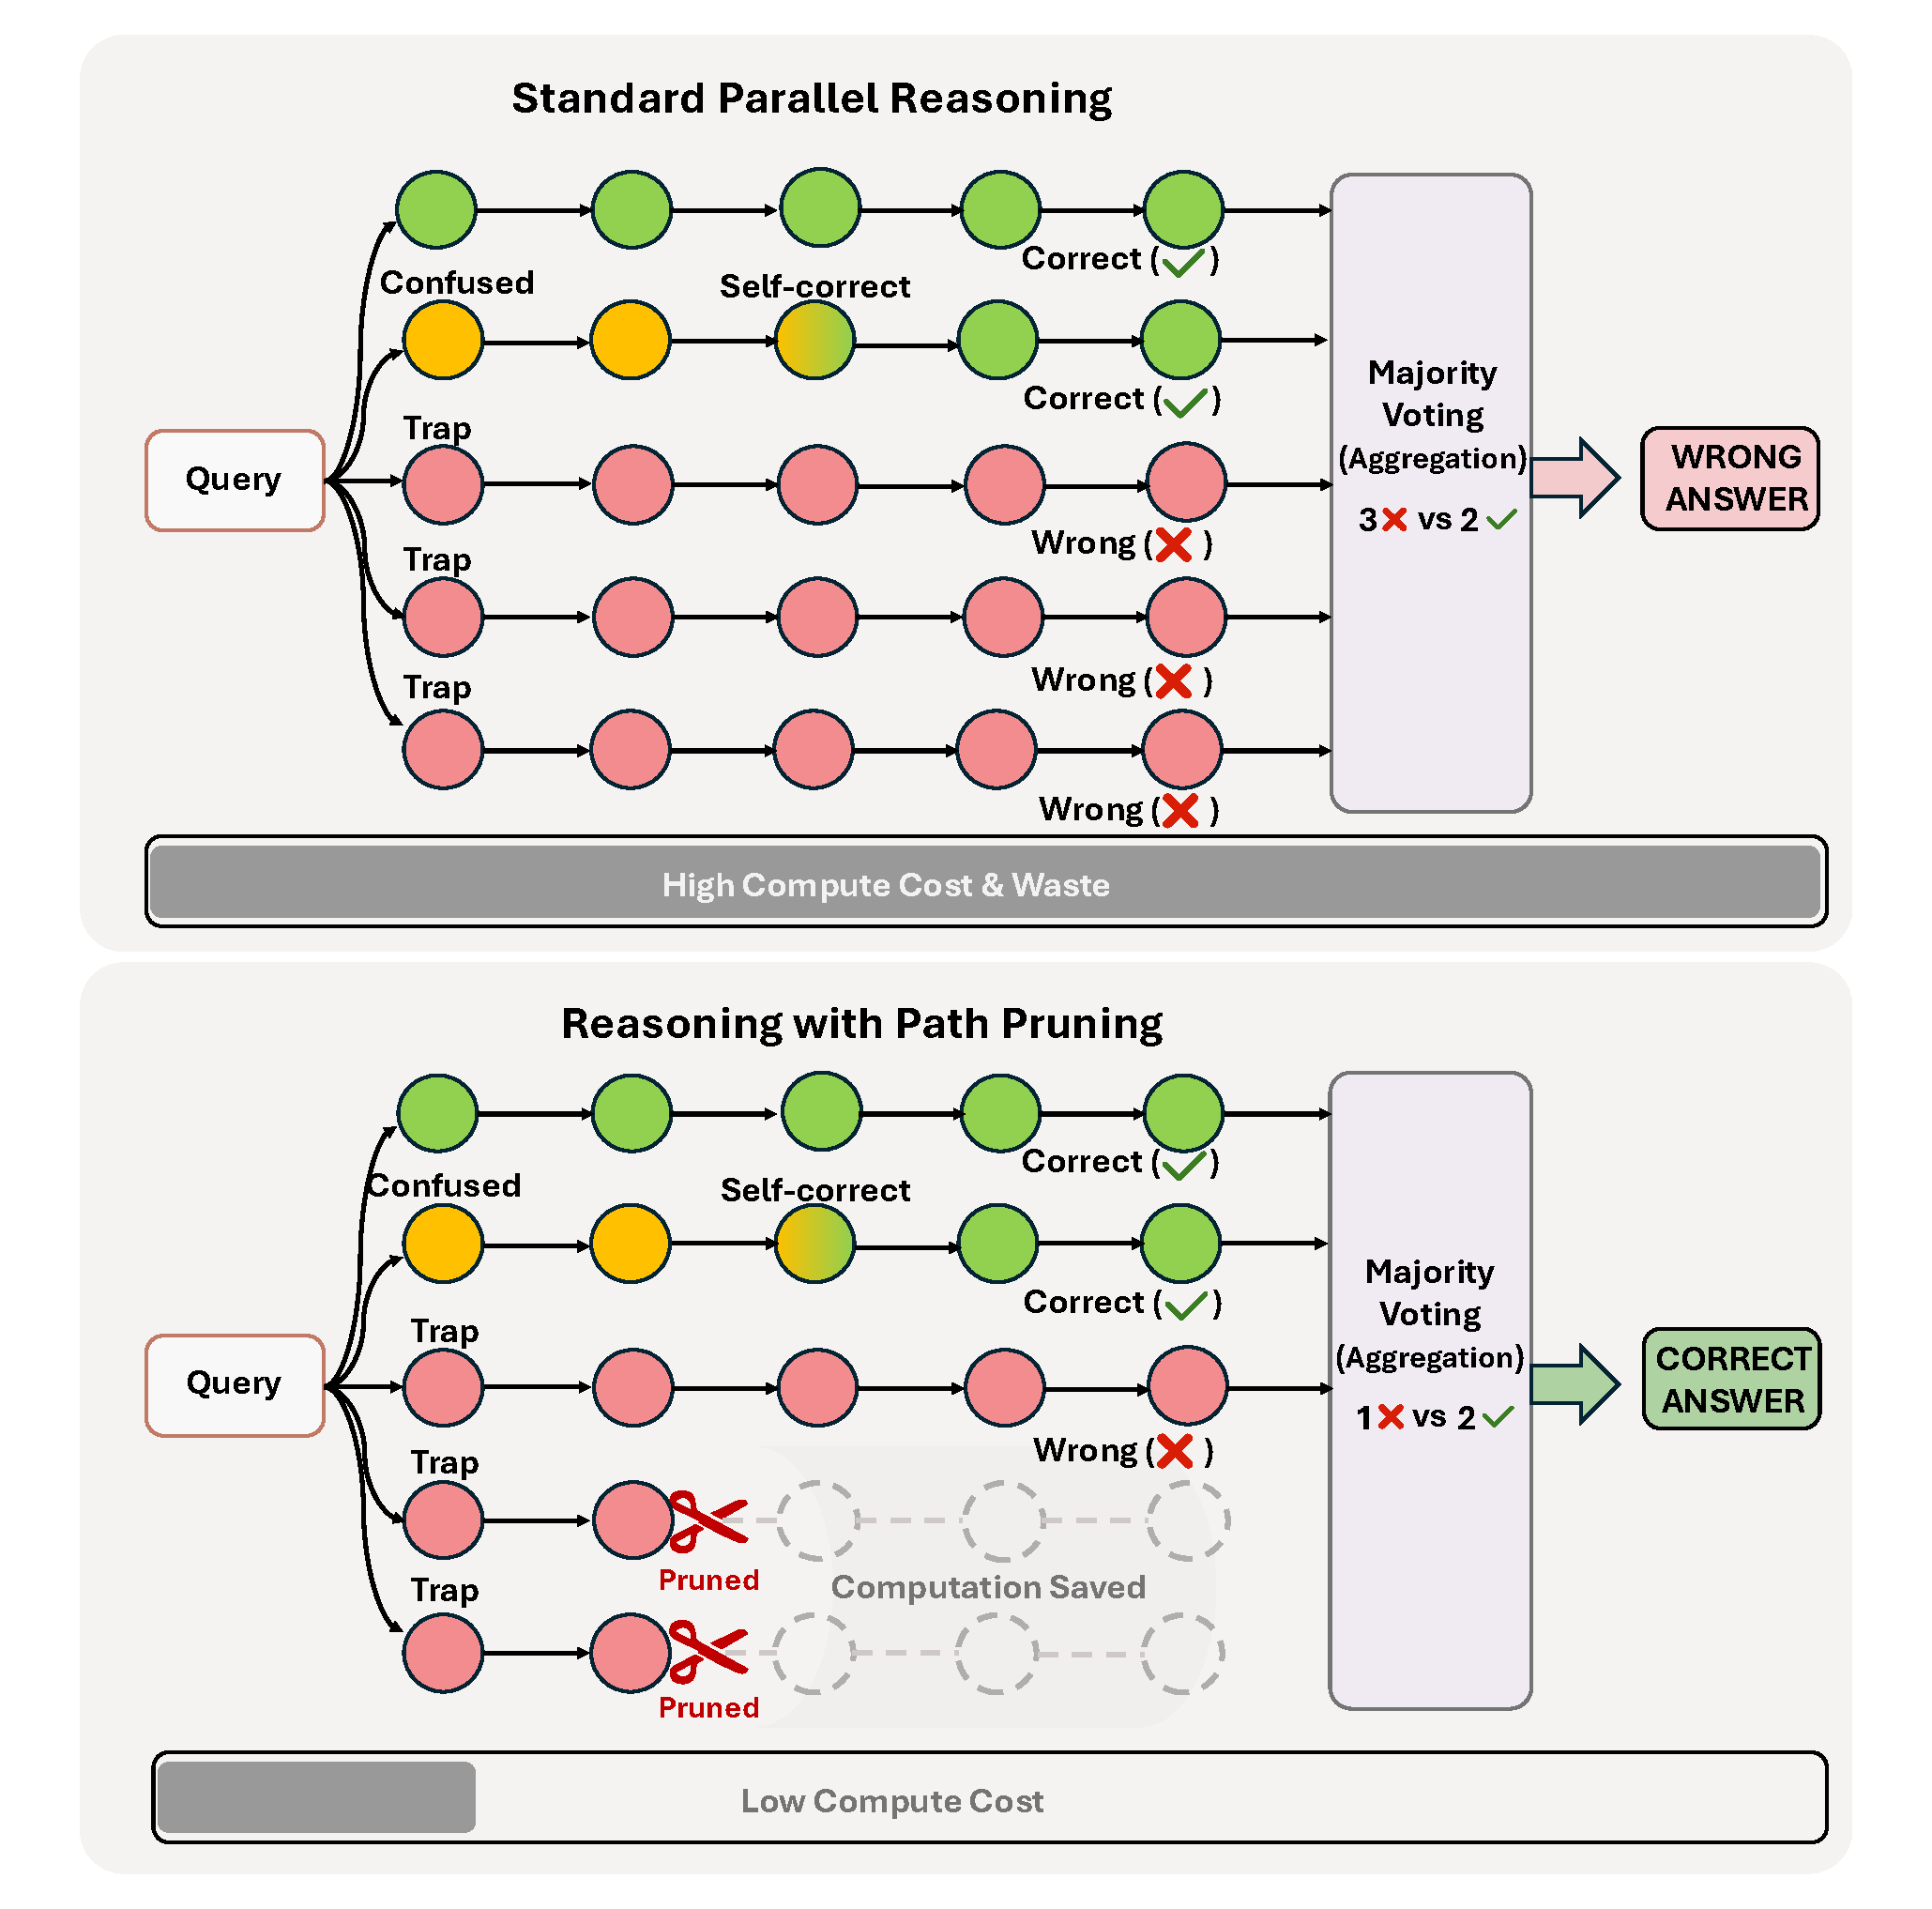
\includegraphics[width=\linewidth]{figures/motivation.pdf} 
    \caption{The necessity of pruning early. Early errors often lead to irreversible failure. Pruning these futile paths early not only saves computation but also purifies the candidate set for better consensus.}
    \label{fig:motivation}
    \vspace{-6mm}
\end{figure}

\paragraph{Why Prune Early in Parallel Reasoning?}
Crucially, recent studies~\cite{luo2025peers,hassid2025short} reveal that this extensive computation is largely squandered: \textbf{not every path contributes to the solution}.
Many trajectories are flawed from inception, yet they consume equal resources to generate and subsequently pollute the final answer aggregation.
As illustrated in Figure~\ref{fig:motivation}, once a reasoning path begins with a flawed prefix, the LRM struggles to self-correct, inevitably spiraling into a futile trajectory~\cite{luo2025peers}.
Consequently, identifying and terminating these unpromising paths at the \textit{prefix level}—a technique known as \textbf{path pruning~(or prefix rejection)}—is essential.

\paragraph{A Unified Taxonomy}
While existing methods attempt to filter paths using auxiliary reward models~\cite{liao2025lost}, internal confidence~\cite{fu2025deepthink}, or semantic redundancy~\cite{hong2025slimsc}, they lack a standardized evaluation protocol, leading to fragmented research.
So first, we propose the first systematic taxonomy of path pruning, classifying methods based on the \textit{source} (internal vs. external) and \textit{learnability} (learnable vs. non-learnable) of their signals (see Figure~\ref{fig:main}).
This taxonomy reveals a significant research gap: the unexplored potential of \textit{learnable internal methods}.
Conceptually, learnable internal methods offer unique advantages, as learning enables task-specific accuracy gains, while internal signals provide early, fine-grained indicators of reasoning failure without incurring extra computational overhead.
To bridge this gap, we introduce \textbf{STOP} (\textbf{S}uper \textbf{TO}ken for \textbf{P}runing), the first efficient instantiation of this paradigm.
Extensive evaluations demonstrate that STOP outperforms existing baselines in both effectiveness and efficiency.

\paragraph{Further Evaluation and Empirical Analysis}
Despite the promise of path pruning, its widespread adoption is currently hindered by unverified scalability across varying computational budgets and model sizes; and the absence of empirical guidelines for determining optimal pruning configurations in real-world scenarios.
To overcome them, we rigorously validate the utility of path pruning in practical settings.
We conduct extensive experiments across diverse model sizes (1.5B to 20B) and compute budgets, confirming that STOP exhibits robust scalability.
Moreover, we distill our empirical analysis into actionable guidelines, providing a formalized method to determine the optimal retention ratio for varying resource constraints.

\paragraph{Contributions}
In summary, this work makes four primary contributions:
(1) We present the first systematic investigation and taxonomy of path pruning.
(2) We propose STOP, a novel pruning method based on learnable internal signals.
(3) We provide a comprehensive evaluation demonstrating STOP's superior scalability and effectiveness.
(4) We establish empirical guidelines to support the practical implementation of path pruning.


\begin{figure}[ht]
% \vspace{-14mm}
  \centering
  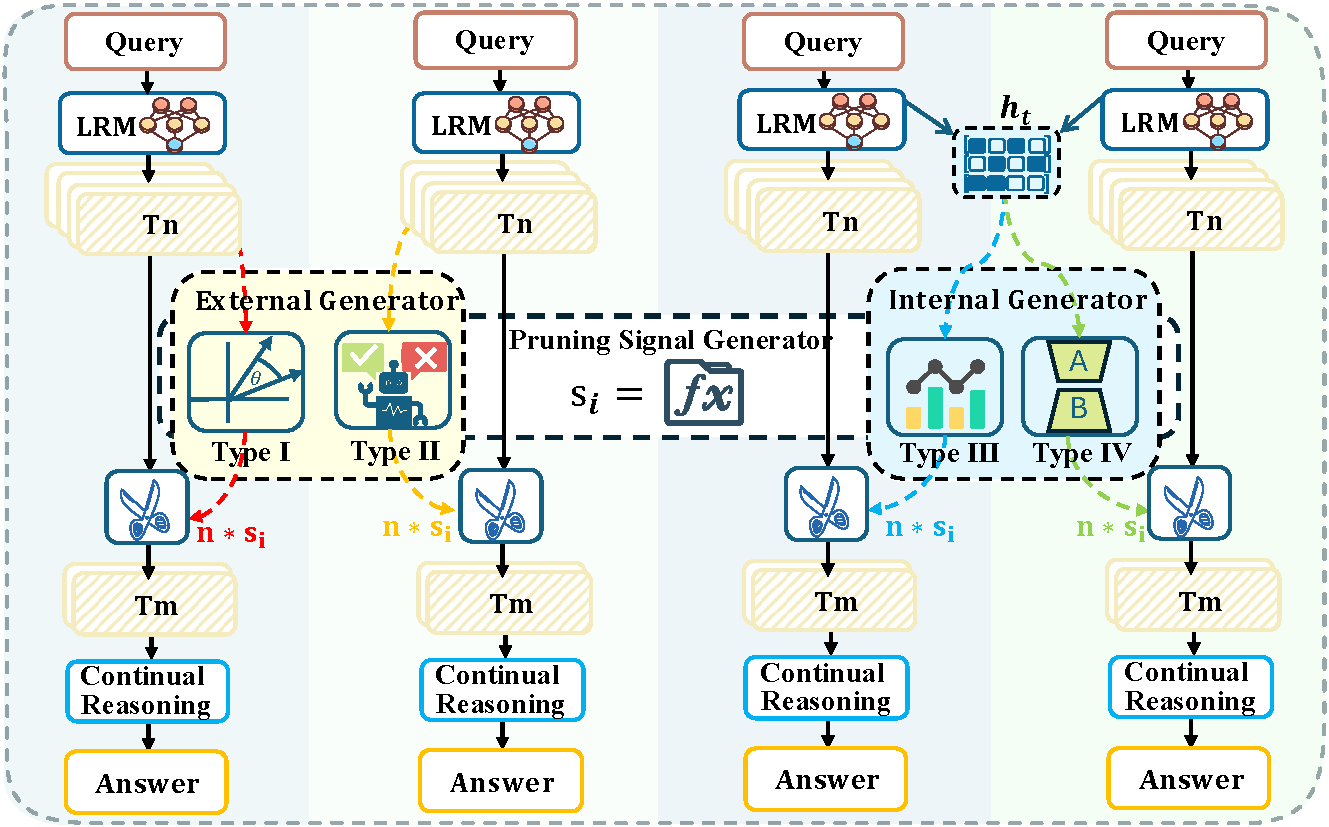
\includegraphics[width=\linewidth]{figures/main.pdf}
  \caption{The proposed taxonomy of path pruning.}
  \label{fig:main}
\vspace{-4mm}
\end{figure}


\section{A Unified Taxonomy of Path Pruning}\label{sec:Four Types}
\subsection{Problem Definition}
\label{subsec:definition}
% 一句话+1-2个公式，cosnider xxx, parallel reasoning is ...

% path pruning is xxx
% \paragraph{The parallel reasoning paradigm.}
Consider a LRM $\Theta$ and an input query $x$, parallel reasoning improves accuracy by generating $N$ independent trajectories $T = \{\tau_i\}_{i=1}^N$, where $\tau_i \sim P_{\Theta}(x)$, and aggregating them through a consensus strategy, such as majority voting.
The final prediction $\hat{y}$ is typically computed as:
\begin{equation}\small
    \hat{y} = \text{vote}(\{\tau_i\}_{i=1}^N).
\end{equation}
However, generating $N$ complete trajectories incurs a linear computational cost ($C \propto N$).
To mitigate this cost, path pruning aims to identify and discard unpromising trajectories early in the decoding process.

% \paragraph{Pruning Signal Generator for Path Pruning}
\paragraph{The Path Pruning Formulation}
Formally, we define a checkpoint at length $L_\text{prefix}$ where the generation is paused.
At this stage, the model has produced a set of prefixes $\mathcal{P} = \{p_i\}_{i=1}^N$.
The core of path pruning is a \textbf{pruning signal generator} $S$, which maps each prefix to a scalar score representing its potential correctness:
\begin{equation}\small
    s_i = S(p_i \mid x, \Theta),
\end{equation}
where $s_i \in [0, 1]$ denotes the pruning signal.
Based on these signals, we retain only the top-$k$ promising paths (where $k \ll N$) for full completion, discarding the rest.
The final aggregated answer is then derived exclusively from this pruned subset:
\begin{equation}
    \hat{y}_\text{pruned} = \text{vote}(\{\text{finish}(p_i) \mid s_i \in \{s_j\}_{j=1}^k\}).
\end{equation}
So, the objective of path pruning is to design an $S$ that maximizes $\hat{y}_\text{pruned}$'s accuracy while minimizing the computational cost (the number of generated tokens).
Therefore, the design of $S$ dictates the effectiveness of the entire framework.


% Recent studies~\cite{hong2025slimsc,liao2025lost,tu2025deepprune,khalifa2025process,lifshitz2025multi,chang2025step,fu2025deepthink,sharma2025thinkjust,he2025adadec} extensively explore this direction and demonstrate the effectiveness of path pruning for improving efficiency.
% From these works, we identify the \emph{critical component} of path pruning as the \textbf{pruning signal generator} ($S$), which scores the potential quality of a partial reasoning trace.
% Formally, given a prefix $\tau_i$, the generator produces a quality signal:
% \begin{equation}
%     s_i = S(\tau_i), \quad s_i \in [0, 1].
% \end{equation}
% Based on these signals, a selection policy retains only the top-$M$ candidates, where $M < N$, and discards the remaining trajectories.
% As a result, the effectiveness of any pruning method fundamentally depends on the design of $S$.

% \subsection{A Unified Taxonomy of Signal Generators}
% \label{sec:taxonomy}

% \begin{table*}[t]
% \small
% \centering
% \caption{A Unified Taxonomy of Path Pruning Methods. We categorize existing works based on the signal source and the generator's learnability.}
% \label{tab:taxonomy}
% \renewcommand{\arraystretch}{1.2} % 稍微增加行高，让列表更舒展
% \resizebox{\linewidth}{!}{
% \begin{tabular}{l|l|l}
% \toprule
%  & \textbf{External Signal Source} & \textbf{Internal Signal Source (Desideratum \ref{desideratum:internal})} \\ \midrule
% \textbf{Non-Learnable} & \begin{tabular}[c]{@{}c@{}}
% Type~\ref{type:Heuristic}\textbf{SlimSC}~\cite{hong2025slimsc}
% \end{tabular} & \begin{tabular}[c]{@{}c@{}}
% \textbf{DeepConf}~\cite{fu2025deepthink} \\
% \textbf{Think Just Enough}~\cite{sharma2025thinkjust} \\
% \textbf{AdaDec}~\cite{he2025adadec}
% \end{tabular} \\ \midrule
% \textbf{\begin{tabular}[c]{@{}c@{}}Learnable\\ (Model-Based) (Desideratum \ref{desideratum:learnable})\end{tabular}} & \begin{tabular}[c]{@{}c@{}}
% \textbf{PRMs}~\cite{chang2025step} \\
% \textbf{DeepPrune}~\cite{tu2025deepprune} \\
% \textbf{Liao et al.}~\cite{liao2025lost} \\
% \textbf{ThinkPRM}~\cite{khalifa2025process} \\
% \textbf{MAV}~\cite{lifshitz2025multi}
% \end{tabular} & \begin{tabular}[c]{@{}c@{}}
% \textbf{STOP (Ours)}
% \end{tabular} \\ \bottomrule
% \end{tabular}
% }
% \end{table*}

% % \paragraph{The nature of the generator.}
% While the mechanism of using this signal is straightforward, the fundamental difference between methods lies in \textit{how this signal is produced}—in other words, the nature of the generator $S$ itself.
% By investigating previous works, as summarized in Table~\ref{tab:taxonomy},
% % we classify four types of \textbf{Pruning Signal Generators ($S$)}:

% We expect two Desiderata:

% \begin{desideratum}\label{desideratum:internal}
% \textbf{internal} an ideal $S$ must can leverage the rich internal information of LRMs.
% \end{desideratum}


% \begin{desideratum}\label{desideratum:learnable}
% \textbf{learnable} an ideal $S$ must can learn to gain better ability.
% \end{desideratum}

% External and  Internal~  


% \paragraph{External Signal Source } ~~~~~ learnable and non-learnable

% \begin{type} \label{type:Heuristic}
% \textbf{Heuristic XX} produce pruning signals using a human pre-designed, non-learnable heuristic function based on the reasoning path, denoted as $S_\text{heuristic}$~\cite{hong2025slimsc};
% \end{type}

% \begin{type}
% \textbf{(B)} employ a trained, external auxiliary model to score the path, denoted as $S_\text{aux}$, utilizing trained reward models to score the generated text~\cite{liao2025lost};
% \end{type}


% \paragraph{Internal  Signal Source } ~~~~~ learnable and non-learnable


% \begin{type}
% \textbf{(C)} apply a pre-designed, non-learnable function (e.g., a confidence metric) to the model's internal states, denoted as $S_\text{stats}$~\cite{fu2025deepthink};
% \end{type}

% \begin{type}\label{type:module}
% and \textbf{(D)} insert a trainable internal module into the reasoning model itself to learn to process these internal states, denoted as $S_\text{module}$.
% \end{type}

\subsection{A Unified Taxonomy of Pruning Signal Generators}
\label{sec:taxonomy}

\begin{table*}[t]
\vspace{-12mm}
\centering
\caption{A Unified Taxonomy of Path Pruning Methods. We categorize methods based on the pruning signal source and learnability. \textbf{Type~\ref{type:module}} satisfies both \textbf{Desideratum~\ref{desideratum:internal}} (Internal) and \textbf{Desideratum~\ref{desideratum:learnable}} (Learnable).}
\label{tab:taxonomy}
\renewcommand{\arraystretch}{1.5} % Increase row height for readability
\resizebox{0.9\linewidth}{!}{
\begin{tabular}{l|c|c}
\toprule
 & \textbf{Non-Learnable} & \textbf{Learnable} \\
 &  & (Desideratum~\ref{desideratum:learnable}) \\ \midrule

\textbf{External Source} & \textbf{Type~\ref{type:heuristic}} & \textbf{Type~\ref{type:aux}} \\
 & \begin{tabular}[c]{@{}c@{}}
\textbf{SlimSC}~\cite{hong2025slimsc}
\end{tabular} & \begin{tabular}[c]{@{}c@{}}
\textbf{DeepPrune}~\cite{tu2025deepprune}, \textbf{LaBoR}~\cite{liao2025lost} \\
\textbf{ThinkPRM}~\cite{khalifa2025process}, \textbf{MAV}~\cite{lifshitz2025multi}
\end{tabular} \\ \midrule

\textbf{Internal Source} & \textbf{Type~\ref{type:stats}} & \textbf{Type~\ref{type:module}} \\
(Desideratum~\ref{desideratum:internal}) & \begin{tabular}[c]{@{}c@{}}
\textbf{DeepConf}~\cite{fu2025deepthink}, 
\textbf{AdaDec}~\cite{he2025adadec} \\
\textbf{Think Just Enough}~\cite{sharma2025thinkjust}
\end{tabular} & \begin{tabular}[c]{@{}c@{}}
\textbf{STOP (Ours)},
\textbf{OTV}\footnotemark~\cite{zhuang2026one}
\end{tabular} \\ \bottomrule
\end{tabular}
}
\vspace{-4mm}
\end{table*}

As defined in Section~\ref{subsec:definition}, the efficacy of path pruning hinges entirely on the quality of the pruning signal generator $S$.
While the function of $S$ is consistent—scoring prefixes—existing methods differ fundamentally in \textit{how} this signal is produced.
To systematically evaluate these approaches, we categorize them based on two critical dimensions: the \textit{source} of the signal (External vs. Internal) and the \textit{learnability} of the generator (Learnable vs. Non-learnable), as summarized in Table~\ref{tab:taxonomy}.

\paragraph{Two Desiderata for Signal Generators}
Before categorizing specific methods, we establish two desiderata for an ideal signal generator:

\begin{desideratum}\label{desideratum:internal}
\textbf{Internal Source} An ideal $S$ should leverage the rich, high-dimensional internal states of the LRM.
\end{desideratum}
Internal signals contain fine-grained information about uncertainty and reasoning dynamics that are often lost in the final text output used by external methods.

\begin{desideratum}\label{desideratum:learnable}
\textbf{Learnability} An ideal $S$ should be trainable to adapt to specific data distributions.
\end{desideratum}
Learnable parameters allow the generator to capture complex, non-linear patterns of error that rigid, pre-defined heuristics cannot model.

Based on these axes, we classify existing works into four distinct types.

\paragraph{External Signal Source}
Methods in this category derive pruning signals from the generated textual output or by querying separate models. They fail to satisfy Desideratum~\ref{desideratum:internal}.

\begin{type}\label{type:heuristic} \textbf{Surface Heuristics}
These methods rely on human-designed rules (e.g. similarity) applied to the surface form of the generated text.
\end{type}
While computationally cheap, these heuristics are rigid and blind to the model's actual confidence.
To overcome these, the next type introduces learnability into the external evaluation process.

\begin{type}\label{type:aux} \textbf{External Judges}
These approaches employ a separate, trained model to evaluate the reasoning path.
\end{type}
Although they satisfy Desideratum~\ref{desideratum:learnable}, they incur significant computational overhead due to the need for additional model inference and fail to access the LRM's internal certainty.
To overcome this rigidity, the next category introduces learnability into the external evaluation process.

\paragraph{Internal Signal Source}
Methods in this category extract signals directly from the LRM's internal states, accessing to richer information (satisfying Desideratum~\ref{desideratum:internal}).

\begin{type}\label{type:stats} \textbf{Raw Confidence}
This paradigm utilizes intrinsic metrics directly derived from the decoding process, such as perplexity or token probability.
\end{type}
However, these methods rely on fixed definitions of confidence, violating Desideratum~\ref{desideratum:learnable}; raw probability does not always correlate with reasoning correctness.

\begin{type}\label{type:module} \textbf{Learned Intuition}
The final category represents the intersection of both desiderata: a trainable module inserted into the LRM to process internal states.
\end{type}
This approach can leverage rich hidden representations (Internal) while adapting to the specific error patterns of the task (Learnable).

\footnotetext{We respectfully note that OTV is our concurrent work, and they are also the first Type IV method.}

% We compare the four proposed $S$ in Figure~\ref{fig:main}.
% While the first three generators are well-represented, $S_\text{module}$ remains, to the best of our knowledge, entirely unexplored. This leaves the fourth and arguably most promising paradigm—one that could theoretically combine learnable accuracy with internal efficiency—as a critical, unaddressed gap.

\section{Methodology: Super Token for Pruning}

% As mentioned earlier, Type~\ref{type:module} offers a promising yet underexplored direction.
% In this section, we introduce \textbf{\textbf{STOP}} (\textbf{S}uper \textbf{TO}ken for \textbf{P}runing), which provides the first efficient instantiation of Type~\ref{type:module} 
% We first present the motivation in Section~\ref{subsec:motivation}, and then describe the design of the \textbf{\textbf{STOP}} module in Section~\ref{subsec:architecture}.

As established in our taxonomy, Type~\ref{type:module} represents the ideal pruning paradigm but remains unexplored.
In this section, we introduce \textbf{STOP} (\textbf{S}uper \textbf{TO}ken for \textbf{P}runing), the first efficient instantiation of this paradigm.
We delineate the motivation in Section~\ref{subsec:motivation}, followed by the architectural design and workflow in Section~\ref{subsec:architecture}.
% Finally, we detail the training and inference protocols in Section~\ref{subsec:protocol}.

\subsection{Motivation for Type~\ref{type:module} Pruning}\label{subsec:motivation}
As illustrated in Figure~\ref{fig:main}, prior methods compromise on either information richness or adaptability.
Type~\ref{type:aux} suffers from high latency, while Type~\ref{type:stats} lacks the capacity to model complex error patterns.
Type~\ref{type:module} represents an ideal optimum: it combines the \textit{efficiency} of accessing internal states with the \textit{adaptability} of learnable parameters.
However, this type remains unexplored due to the challenge of designing a module that extracts these signals without disrupting the LRM's generative capabilities.



\begin{figure*}[ht]
\vspace{-12mm}
    \centering
    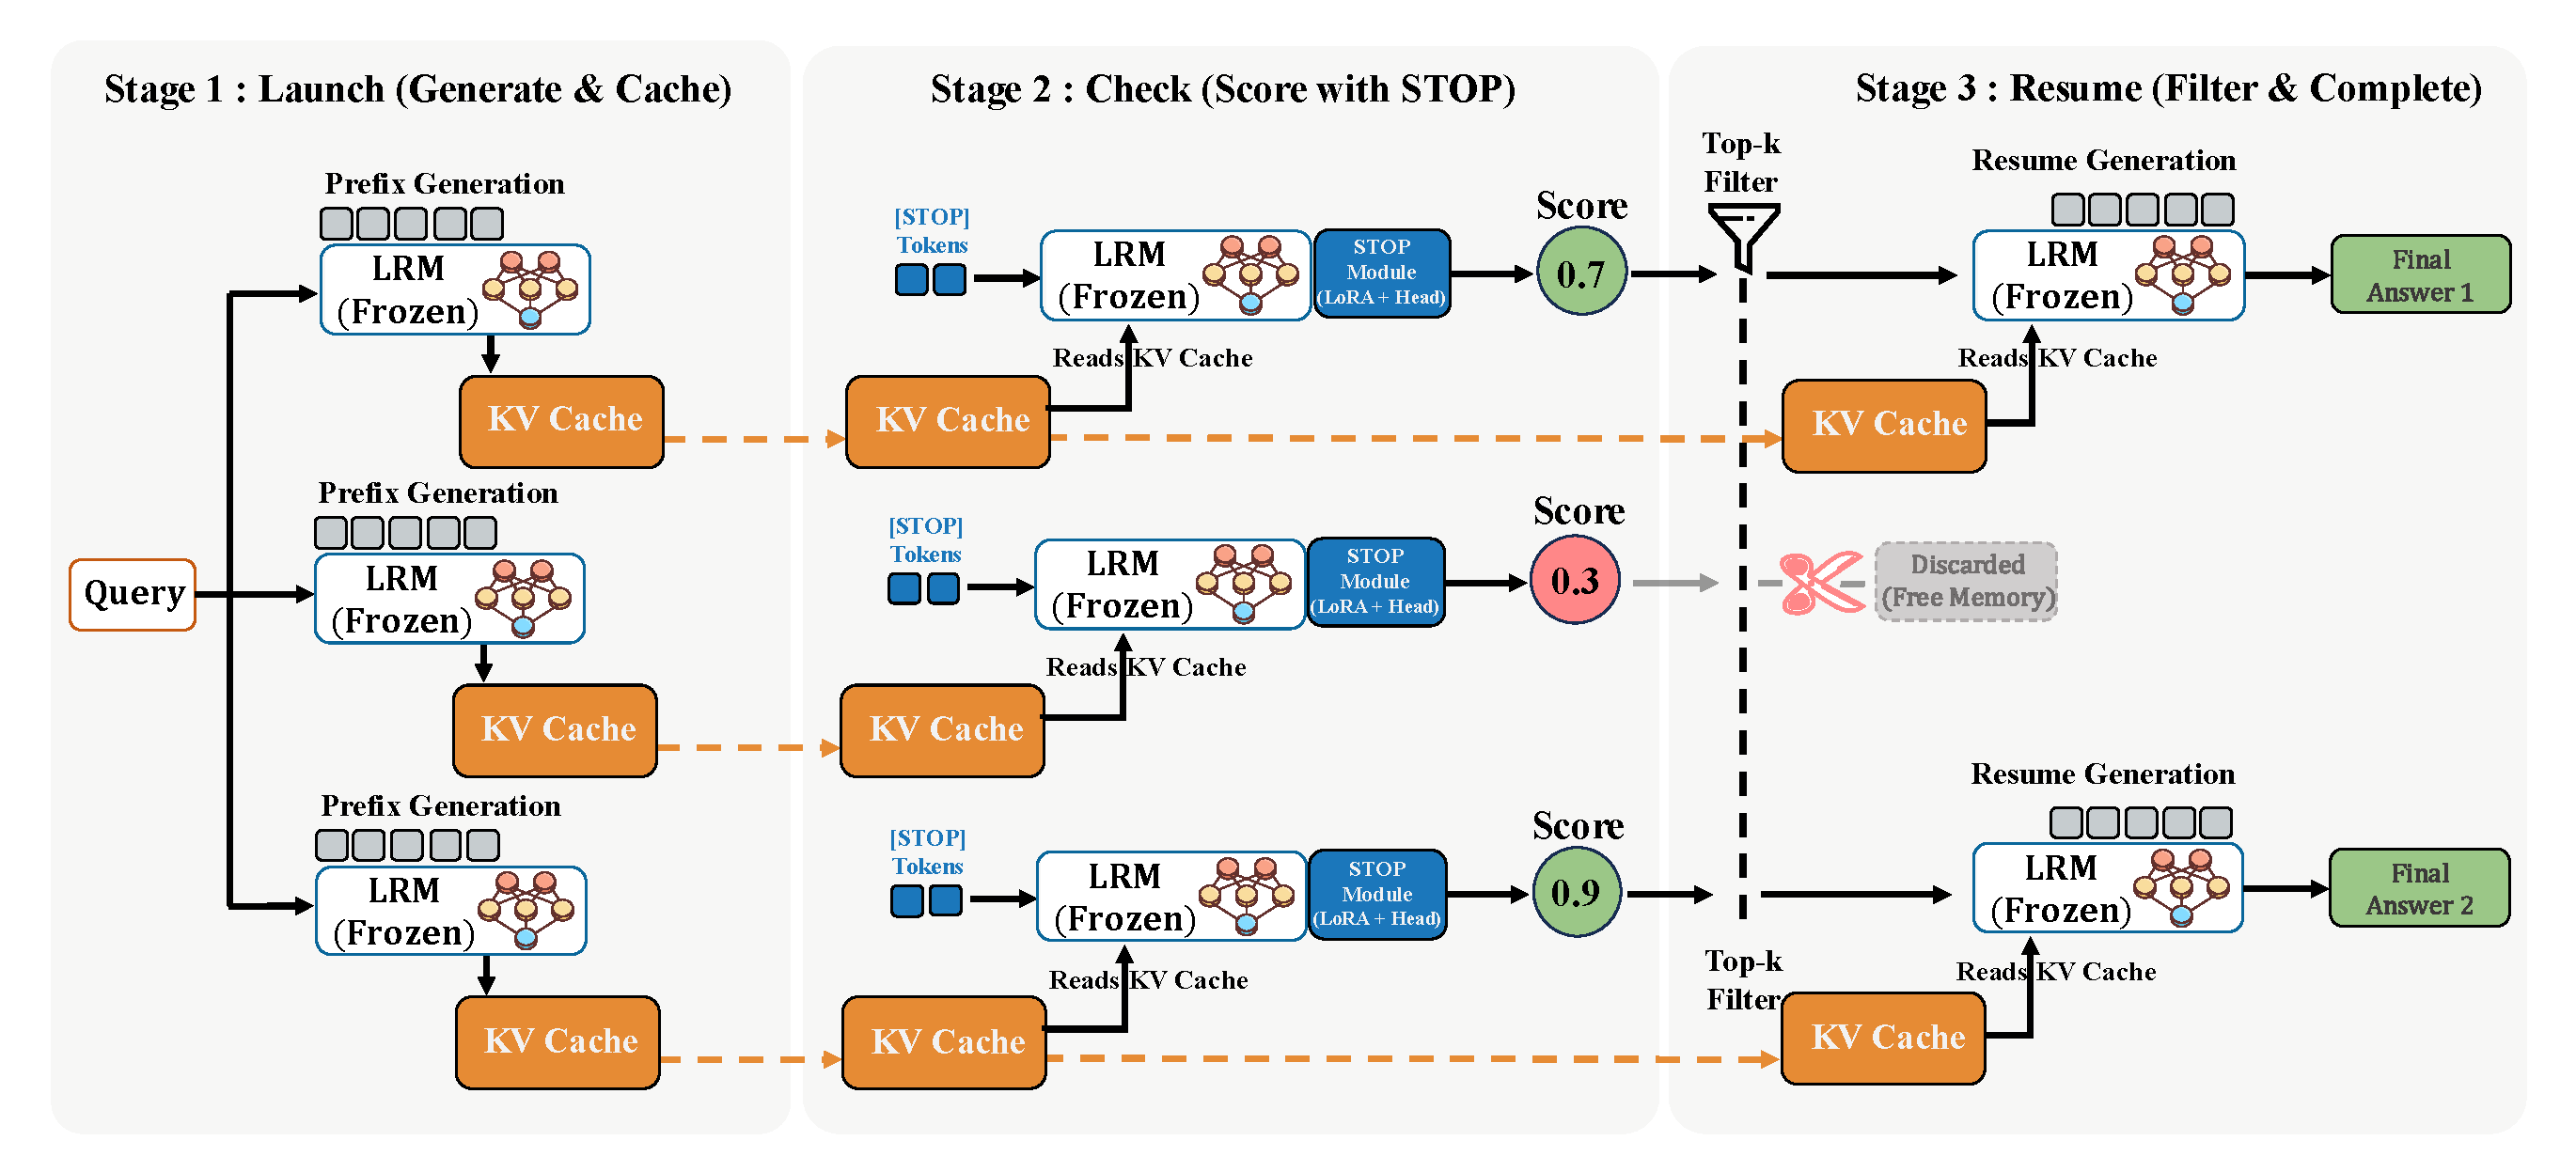
\includegraphics[width=\textwidth]{figures/method.pdf}
    \caption{The inference process comprises three stages: caching initial prefixes (\textbf{Launch}), scoring them via the \textbf{STOP} module (\textbf{Check}), and completing only the top-ranked candidates (\textbf{Resume}).}
    \label{fig:method_STOP}
\vspace{-4mm}
\end{figure*}


\subsection{Instantiation of Type~\ref{type:module} Pruning: STOP}
\label{subsec:architecture}

To instantiate this type, we design \textbf{STOP} as a lightweight, non-invasive module that integrates seamlessly with the backbone LRM.

\paragraph{Components}
We augment the fixed LRM $\Theta$ with three learnable components:
(1) \textbf{A Super Token (\texttt{[STOP]})} added to the vocabulary, acting as a specialized query vector to aggregate information;
(2) \textbf{A Critique Adapter} LoRA ($\theta_\text{LoRA}$), activated only when processing the \texttt{[STOP]} token to extract error-specific features without altering the LRM's general reasoning capabilities;
(3) \textbf{A Classification Head} ($W_\text{cls}$), which projects the hidden state of the \texttt{[STOP]} token to a scalar probability.

This design ensures \textbf{modularity}: the original parameters $\Theta$ remain frozen, preserving the LRM's generative capability while enabling efficient parameter-efficient fine-tuning (PEFT).

\paragraph{Training: Learn to Use Internal Information}
The goal of training is simple: teach the model to distinguish promising prefixes from futile ones.
Formally, for a prefix $p_i$, we derive a soft label $s^{mc}_i \in [0,1]$ via Monte Carlo estimation (details in Appendix~\ref{app:data_construction}).
The training process involves two steps:
First, we compute the KV cache of the prefix using the frozen LRM: $\mathcal{C}_{p_i} = \text{LRM}(p_i; \Theta)$.
Second, we append a sequence of learnable \texttt{[STOP]} tokens, denoted as $T_s$, and process them using the LoRA-augmented model.
The final hidden state $h_i$ is fed into the classifier to minimize the soft binary cross-entropy loss:
\begin{equation}\small
\begin{array}{ll}
    \mathcal{L} = & - [ s_i^{mc} \log \sigma (W_{cls}h_i) \\
    & +  (1-s_i^{mc}) \log (1-\sigma (W_{cls}h_i)) ],
\end{array}
\end{equation}
where $h_i = \text{LRM}(T_s \mid \mathcal{C}_{p_i}; \Theta, \theta_{\text{LoRA}})_{-1}$.

\paragraph{Training Cost}
Constructing the MC supervision requires sampling multiple continuations per prefix to estimate $s^{mc}_i$ (e.g., $K=32$), which introduces an upfront computational cost during data construction. However, this cost is incurred only once, and the resulting STOP module is lightweight and reusable across tasks. To facilitate transparency and reproducibility, we provide detailed cost statistics in Appendix~\ref{app:training_cost} and will release the constructed dataset and trained checkpoints, allowing practitioners to bypass this step entirely. Importantly, this one-time cost is amortized during deployment, where STOP improves efficiency by pruning unpromising paths early.

\paragraph{Inference: ``Launch-Check-Resume''}
To efficiently prune paths without slowing down generation, we design a three-stage pipeline (Figure~\ref{fig:method_STOP}):

\textbf{Stage 1: Launch}
Instead of generating the full trajectories immediately, we first generate $N$ short prefixes (e.g., first 1024 tokens) for the query.
Crucially, we cache the internal states (KV Cache) of these prefixes.

\textbf{Stage 2: Check}
We append the \texttt{[STOP]} tokens to the cached prefixes.
The trained module reads the KV cache and outputs a quality score for each prefix.
\textit{Note:} This step is extremely fast because it processes only a few tokens (the \texttt{[STOP]} sequence) and reuses the heavy computation already done in Stage 1.

\textbf{Stage 3: Resume}
We rank the prefixes by their scores and apply a \textbf{Top-$k$ Filter}.
Futile paths are discarded immediately to free up memory.
Only the top-$k$ most promising prefixes are resumed and generated to completion to obtain the final answers.

% \subsection{Probing the ``Subconscious'' of LRMs}
% \label{subsec:intuition}

% % As mentioned earlier, the $S_\text{module}$ paradigm offers a promising yet underexplored direction. 
% % \tx{motivation: the final output is not true thinking of LRMs -> leverage the internal states in LRMs -> KV caches are richer than last hidden -> this inspire us ....}
% \paragraph{The illusion of explicit reasoning.}
% Recent study~\cite{shojaee2025illusion} identifies a key discrepancy: the explicit reasoning chain produced by an LRM is only a low-dimensional, discrete projection of its high-dimensional internal states.
% During this projection, important epistemic signals, such as uncertainty spikes associated with reasoning collapse, are compressed or lost.
% Therefore, accurately estimating the quality of a reasoning trajectory requires bypassing this textual bottleneck and directly leveraging internal representations.

% \paragraph{Richer representations in KV cache.}
% This observation motivates a focus on the \textbf{key--value (KV) cache}.
% Unlike the final hidden state, which provides a local summary of the immediate context, the KV cache preserves the full activation history of the reasoning process.
% It serves as a holistic record of cognitive dynamics and retains fine-grained traces of algorithmic execution that are often obscured in surface text.
% Based on this insight, we design a mechanism that directly probes this latent logical history.



% 需要和上面的motivation衔接好
% \subsection{Instanliz of Type~\ref{type:module} Pruning: STOP}
% \label{subsec:architecture}

% Given the dataset of \texttt{(prefix, $s^{mc}$)} pairs, our goal is to train an efficient module that predicts the success probability of a prefix.
% We introduce \textbf{STOP} (Super Token for Pruning), a module that evaluates internal states (Key-Value Cache) without interfering with the model's native reasoning.
% \paragraph{Probabilistic supervision.}

% overall statement: 总分总？
% 方法 和 实现 分离开？


% To translate the intuition of probing the ``subconscious'' into a concrete mechanism, we introduce \textbf{\textbf{STOP}} (\textbf{S}uper \textbf{TO}ken for \textbf{P}runing).
% This module directly evaluates the internal Key-Value Cache without interfering with the model's native reasoning.
% Formally, we train \textbf{STOP} using \texttt{(prefix, $s^{mc}$)} pairs to predict the success probability $s^{mc}$, a probabilistic soft label derived via Monte Carlo estimation (see Appendix~\ref{app:data_construction} for details).

% \paragraph{Architecture.}
% We augment the LRM with two components:
% \textbf{(1) Super Token [STOP]}, a new special token added to the vocabulary with a unique classifier head in the final output layer.
% \textbf{(2) Light-Expert LoRA}, a low-rank adapter applied only to \texttt{[STOP]}, specializes in extracting errors from prefixes.

% \paragraph{Training STOP efficiently.}
% Given a sample $(p_i, s^{mc}_i)$, we first pass the prefix $p_i$ to the LRM with parameters $\Theta$ to obtain its Key-Value Cache (KV Cache) $\mathcal{C}_{p_i}$:
% \begin{equation}\small
%     \mathcal{C}_{p_i} = \text{LRM}(p_i; \Theta)
% \end{equation}
% Subsequently, a sequence of \texttt{STOP} tokens, denoted as $T_s$, is passed into the model with the trainable LoRA.
% The hidden state of the last token of $T_s$ from the final transformer layer is fed into a classifier with parameters $W_{cls}$. We minimize the loss to train the embeddings of $T_s$, $W_{cls}$, and $\theta_{LoRA}$:
% \begin{equation}\small
% \begin{array}{ll}
%     \mathcal{L} = & - [ s_i^{mc} \log \sigma (W_{cls}h_i) \\
%     & +  (1-s_i^{mc}) \log (1-\sigma (W_{cls}h_i)) ]
% \end{array}
% \end{equation}
% where $h_i=\text{LRM}(T_s;\mathcal{C}_{p_i};\Theta,\theta_{LoRA})_{-1}$ is the hidden state of the last token of $T_s$ in the final layer.

% \paragraph{Accelerating inference with STOP.}
% After training, we obtain the optimized \texttt{STOP} tokens, the classifier, and the LoRA adapter.
% During inference, we use these components to produce pruning signals.

% Consider a problem in a basic parallel inference setting, where the goal is to produce $N$ reasoning paths and determine the final answer through majority voting. 
% Instead of generating the full reasoning paths directly, we first stop at a certain prefix length. 
% This produces $N$ prefixes $\{p_1, \dots, p_N\}$ together with their KV caches $\{\mathcal{C}_{p_i}\}_{i=1}^N$.

% Next, we feed the \texttt{STOP} tokens into the model (with LoRA) to obtain the pruning signals $\{s_i\}_{i=1}^N$ for each prefix.
% It is notable that we \textbf{reuse the KV caches $\{\mathcal{C}_{p_i}\}_{i=1}^N$ here to improve efficiency} instead of recomputing them.
% We sort the prefixes and filter them via top-$k$ or top-$p$, discarding the remaining paths.
% Finally, we continue reasoning only for the retained prefixes (without LoRA and \texttt{STOP} tokens) to generate the final answers and perform majority voting.

% Notably, the capability of the LRM remains unchanged, as its parameters $\Theta$ remain frozen during both training and inference.

% \paragraph{Training Process}
% The training follows a non-invasive two-stage procedure. For a training sample $(p_i, s^{mc})$ with prefix length $T_p$:

% \begin{enumerate}[nosep]
%     \item \textbf{Prefix State Encoding.} We first disable the adapter $\phi$ and process $p_i$ with the frozen $\text{LRM}_{\theta}$. Following standard notation, this produces and caches the per-layer key-value states:
%     % \begin{equation}
%     % \mathcal{C}_{p_i} = \left\{ \left( K^{(l)}_{1:T_p}, V^{(l)}_{1:T_p} \right) \right\}_{l=1}^L,
%     % \end{equation}
%     \begingroup
%     \setlength{\abovedisplayskip}{4pt}
%     \setlength{\belowdisplayskip}{4pt}
%     \begin{equation}
%         \mathcal{C}_{p_i} = \left\{ \left( K^{(l)}_{1:T_p}, V^{(l)}_{1:T_p} \right) \right\}_{l=1}^L
%     \end{equation}
%     \endgroup
%     where $K^{(l)}_{1:T_p} = [k^{(l)}_1, \dots, k^{(l)}_{T_p}]$ and $V^{(l)}_{1:T_p} = [v^{(l)}_1, \dots, v^{(l)}_{T_p}]$ denote the concatenated key and value states at layer $l$.

%     \item \textbf{STOP Token Assessment.} Next, we activate the adapter $\phi$ and feed $n$ \texttt{[STOP]} tokens ($T_s$) to the model. These tokens are processed \textbf{using $\mathcal{C}_{p_i}$ as a read-only historical cache}. The final \texttt{[STOP]} token produces a hidden state $h_s$ through $\text{LRM}_{\theta, \phi}$, which is then passed to the head to predict the success probability:
%     % \begin{equation}
%     %     h_s = \text{Process}(\text{LRM}_{\theta, \phi}, T_s, \text{Cache}=\mathcal{C}_{p_i})[-1],
%     % \end{equation}
%     % \begin{equation}
%     %        \hat{y} = \text{softmax}(W_{\text{head}} \cdot h_s).
%     % \end{equation}
%     \begingroup
% \setlength{\abovedisplayskip}{4pt}
% \setlength{\belowdisplayskip}{4pt}
% \begin{equation}
%     h_s = \text{Process}(\text{LRM}_{\theta, \phi}, T_s, \text{Cache}=\mathcal{C}_{p_i})[-1]
% \end{equation}
% \endgroup

% \begingroup
% \setlength{\abovedisplayskip}{8pt}
% \setlength{\belowdisplayskip}{4pt}
% \begin{equation}
%     \hat{y} = \text{softmax}(W_{\text{head}} \cdot h_s)
% \end{equation}
% \endgroup
%     We train the adapter $\phi$ (including $W_{\text{head}}$) with the cross-entropy loss $\mathcal{L}(\phi) = \text{CE}(s^{mc}, \hat{y})$, while keeping $\theta$ frozen.
% \end{enumerate}

% \paragraph{Inference and Pruning Process}
% Our inference pipeline follows a structured three-stage procedure:

% \begin{description}[ labelsep=0.5em, itemsep=0pt, parsep=0pt, topsep=2pt]
%     \noindent \textbf{Generation.} The frozen $\text{LRM}_{\theta}$ generates $N$ candidate paths from an input prompt. At a predefined assessment point, we store each path's prefix cache $\mathcal{C}_{p_i}$ (as defined in Eq.~(1)).
%     \noindent \textbf{Assessment \& Pruning.} We activate the adapter $\phi$. For each of the $N$ paths, we compute its success probability $\hat{y}_i$ (per Eq.~(2--3)) by feeding $n$ \texttt{[STOP]} tokens conditioned on its cache $\mathcal{C}_{p_i}$. We then select the $m$ paths ($m < N$) with the highest scores and prune the rest.
%     \noindent \textbf{Continuation.} We disable $\phi$. For each of the $m$ surviving paths, we retrieve its \textbf{original} prefix cache $\mathcal{C}_{p_i}$ from Stage 1. Generation is then resumed from this exact state using only the frozen $\text{LRM}_{\theta}$ to produce the final output.
% \end{description}

% \noindent \textbf{Generation.}
% The frozen $\text{LRM}_{\theta}$ generates $N$ candidate paths from an input prompt. At a predefined assessment point, we store each path's prefix cache $\mathcal{C}_{p_i}$.

% \noindent \textbf{Assessment \& Pruning.}
% We activate the adapter $\phi$. For each of the $N$ paths, we compute its success probability $\hat{y}_i$ by feeding $n$ \texttt{[STOP]} tokens conditioned on its cache $\mathcal{C}_{p_i}$. We then select the $m$ paths ($m < N$) with the highest scores and prune the rest.

% \noindent \textbf{Continuation.}
% We disable $\phi$. For each of the $m$ surviving paths, we retrieve its \textbf{original} prefix cache $\mathcal{C}_{p_i}$ from Stage 1. Generation is then resumed from this exact state using only the frozen $\text{LRM}_{\theta}$ to produce the final output.
    
% This design ensures computational efficiency. The reasoning capability of the base $\text{LRM}_{\theta}$ remains unchanged as its parameters stay frozen. 

% \begin{figure}[t]
%     \centering

%     % 子图 A
%     \begin{subfigure}{\columnwidth}
%         \centering
%         \includegraphics[height=4.2cm]{figures/method_data_construction.pdf}
%         \caption{Data Construction.}
%         \label{fig:method_data_construction}
%     \end{subfigure}

%     \vspace{0.3cm}

%     % 子图 B
%     \begin{subfigure}{\columnwidth}
%         \centering
%         \includegraphics[height=3.8cm]{figures/method_STOP.pdf}
%         \caption{STOP.}
%         \label{fig:method_STOP}
%     \end{subfigure}

%     \caption{Comparison of the two procedures in our method.}
%     \label{fig:method_two_subfigures}
% \end{figure}


\begin{table*}[ht!]
\vspace{-12mm}
\centering
\caption{
    Results of avg@k (avg@m|k) across various models and benchmarks. 
    The best result in each row is \textbf{bolded} and the second best is \underline{underlined}.
}
\label{tab:main_results}
\resizebox{\textwidth}{!}{% Make the table fit the page width
\begin{tabular}{llcc cc cc cc cc}
\toprule
% \multirow{2}{*}{\textbf{Model}} & \multirow{2}{*}{\textbf{Dataset}} 
% & \multicolumn{2}{c}{\textbf{No pruning (Baseline)}} 
% & \multicolumn{2}{c}{\textbf{$S_\text{heuristic}$ }} 
% & \multicolumn{2}{c}{\textbf{$S_\text{aux}$ }} 
% & \multicolumn{2}{c}{\textbf{$S_\text{stats}$ }} 
% & \multicolumn{2}{c}{\textbf{$S_\text{module}$ }} \\
% \cmidrule(lr){3-4} \cmidrule(lr){5-6} \cmidrule(lr){7-8} \cmidrule(lr){9-10}\cmidrule(lr){11-12}
% & & avg@64 ($\uparrow$) & Tokens ($\downarrow$)  & avg@8|64 ($\uparrow$) & Tokens (\% $\downarrow$) & avg@8|64 ($\uparrow$) & Tokens (\% $\downarrow$) & avg@8|64 ($\uparrow$) & Tokens (\% $\downarrow$)& avg@8|64 ($\uparrow$) & Tokens (\% $\downarrow$) \\
% \midrule
% \midrule
% \multirow{5}{*}{DS-Qwen-2.5-1.5B} 
% & AIME24    & 30.10               & 782.3k  &26.25  & 218.3k~(-72.09\%)  &  32.50             & 325.9k~(-58.34\%) &\underline{32.92}   & \underline{210.6k}~(-73.08\%)    & \textbf{37.92}   & \textbf{204.3k}~(-73.88\%)\\
% & AIME25    & 22.76               & 784.8k  &\underline{24.17}  & 214.7k~(-72.64\%)  &  \underline{24.17} & 325.0k~(-58.59\%) & 23.75              & \underline{208.7k}~(-73.40\%)    & \textbf{26.67}   & \textbf{206.6k}~(-73.68\%)\\
% & BRUMO25   & 30.99               & 774.6k  &29.58  & 212.8k~(-72.53\%)  &  \underline{31.67} & 325.6k~(-57.96\%) & 31.67  & \underline{209.7k}~(-72.93\%)    & \textbf{33.75}   & \textbf{204.4k}~(-73.61\%) \\
% & HMMT25    & 15.05               & 856.4k  &15.83  & 224.2k~(-73.82\%)  &  15.00             & 337.2k~(-60.63\%) &\underline{17.08}   & \underline{220.9k}~(-74.21\%)    & \textbf{17.92}   & \textbf{215.5k}~(-74.84\%)\\
% & GPQA-D    & 33.08               & 550.9k  &32.32  & 187.1k~(-66.03\%)  &  -                 & -                 & \underline{34.98}  & \underline{180.4k}~(-67.25\%)    & \textbf{48.42}   & \textbf{179.4k}~(-67.43\%) \\

% \midrule
% \multirow{5}{*}{DS-Qwen-2.5-7B} 
% & AIME24    &  54.69             & 666.2k  &53.75   & 202.7k~(-69.58\%)  &  54.58              & 312.5k~(-53.09\%) & \underline{55.00}  & \underline{197.4k}~(-70.38\%)    &  \textbf{61.67}  & \textbf{189.0k}~(-71.63\%) \\
% & AIME25    &  39.67             & 703.0k  &35.42   & 207.4k~(-70.50\%)  &  39.17              & 317.6k~(-54.82\%) & \underline{41.67}  & \underline{202.6k}~(-71.18\%)    & \textbf{42.50}   & \textbf{197.5k}~(-71.91\%) \\
% & BRUMO25   &  50.99             & 656.6k  &50.00   & 199.3k~(-69.64\%)  & 51.25               & 312.1k~(-52.46\%) & \underline{52.92}  & \underline{194.5k}~(-70.38\%)    & \textbf{56.67}   & \textbf{190.2k}~(-71.03\%)\\
% & HMMT25    &  23.91             & 808.9k  &\underline{25.00}   & 219.5k~(-72.87\%)  & 23.33               & 330.8k~(-59.11\%) & 24.58  & \underline{216.1k}~(-73.28\%)    & \textbf{27.08}   & \textbf{211.6k}~(-73.84\%)\\
% & GPQA-D    &  45.95             & 443.8k  &\underline{47.09}   & 173.6k~(-60.89\%)  & -                   & -                 & 46.02  & \underline{166.7k}~(-62.43\%)    & \textbf{55.75}   & \textbf{165.9k}~(-62.61\%)\\
% \midrule
% \multirow{5}{*}{DS-Qwen-3-8B} 
% & AIME24    &  76.93             & 1361k   &77.50   & 290.4k~(-78.67\%)  & \underline{78.75}   & 398.4k~(-70.73\%) & 78.33              & \underline{284.3k}~(-79.11\%)    & \textbf{79.17}   & \textbf{279.0k}~(-79.51\%)\\
% & AIME25    &  70.68             & 1427k   &69.17   & 297.2k~(-79.18\%)  &  \underline{72.50}  & 408.4k~(-71.39\%) & 70.42              & \underline{291.2k}~(-79.60\%)    & \textbf{72.92}   & \textbf{290.9k}~(-79.62\%)\\
% & BRUMO25   &  75.00             & 1320k   &\underline{76.25}   & 284.8k~(-78.43\%)  &   75.83 & 394.9k~(-70.10\%) & 74.58              & \underline{280.2k}~(-78.78\%)    & \textbf{78.75}   & \textbf{277.5k}~(-78.98\%)\\
% & HMMT25    &  51.04             & 1601k   &50.00   & 322.1k~(-79.88\%)  & 50.83               & 427.8k~(-73.28\%) & \underline{51.25}  & \underline{314.0k}~(-80.38\%)    & \textbf{54.58}   & \textbf{311.7k}~(-80.53\%)\\
% & GPQA-D    &  56.87             & 652.6k  &57.07   & 201.0k~(-69.20\%)  &  -                  & -                 & \underline{58.78}  & \underline{196.6k}~(-69.86\%)    & \textbf{63.32}   & \textbf{193.5k}~(-70.35\%)\\
% \midrule
% \multirow{5}{*}{GPT-OSS-20B}
% & AIME24    &  75.26             & 594.2k  & 73.33              & 196.6k~(-66.91\%)  & \underline{76.25}  & 299.8k~(-49.55\%) & 75.00              & \underline{187.0k}~(-68.54\%)    & \textbf{77.50}   & \textbf{184.4k}~(-68.98\%) \\
% & AIME25    &  70.99             & 673.4k  & 69.17  & 205.1k~(-69.54\%)  & 69.17              & 311.7k~(-53.71\%) & \underline{70.83}             & \underline{197.7k}~(-70.64\%)    & \textbf{75.42}   & \textbf{191.1k}~(-71.62\%)\\
% & BRUMO25   &  68.02             & 575.6k  &\underline{69.17}   & 187.6k~(-67.41\%)  &  66.25              & 298.8k~(-48.09\%) & 67.92              & \textbf{179.0k}~(-68.90\%)       & \textbf{70.00}   & \underline{183.6k}~(-68.11\%) \\
% & HMMT25    &  \underline{48.13} & 910.8k  &45.83               & 236.3k~(-74.06\%)  &  45.42              & 336.9k~(-63.01\%) & 46.25              & \underline{228.0k}~(-74.97\%)    & \textbf{52.92}   & \textbf{216.1k}~(-76.27\%)\\
% & GPQA-D    &  65.55             & 277.2k  &66.41   & 151.8k~(-45.24\%)  &  -                  & -                 &  \underline{68.43} & \underline{145.9k}~(-47.36\%)    & \textbf{77.46}   & \underline{143.4k}~(-48.26\%)\\

\multirow{2}{*}{\textbf{Model}} & \multirow{2}{*}{\textbf{Dataset}} 
& \multicolumn{2}{c}{\textbf{No pruning (Baseline)}} 
& \multicolumn{2}{c}{\textbf{Type~\ref{type:heuristic} }} 
& \multicolumn{2}{c}{\textbf{Type~\ref{type:aux}}} 
& \multicolumn{2}{c}{\textbf{Type~\ref{type:stats}}} 
& \multicolumn{2}{c}{\textbf{Type~\ref{type:module}}} \\
\cmidrule(lr){3-4} \cmidrule(lr){5-6} \cmidrule(lr){7-8} \cmidrule(lr){9-10}\cmidrule(lr){11-12}
& & avg@64 ($\uparrow$) & Tokens ($\downarrow$)  & avg@8|64 ($\uparrow$) & Tokens (\% $\downarrow$) & avg@8|64 ($\uparrow$) & Tokens (\% $\downarrow$) & avg@8|64 ($\uparrow$) & Tokens (\% $\downarrow$)& avg@8|64 ($\uparrow$) & Tokens (\% $\downarrow$) \\

\midrule
\multirow{5}{*}{DS-Qwen-2.5-1.5B} 
& AIME24    & \cellcolor{mygreen1}30.10 & 782.3k  & \cellcolor{mygreen1}26.25 & 218.3k~(-72.09\%)  & \cellcolor{mygreen2}32.50 & 325.9k~(-58.34\%) & \cellcolor{mygreen2}\underline{32.92} & \underline{210.6k}~(-73.08\%)    & \cellcolor{mygreen3}\textbf{37.92} & \textbf{204.3k}~(-73.88\%)\\
& AIME25    & \cellcolor{mygreen1}22.76 & 784.8k  & \cellcolor{mygreen2}\underline{24.17} & 214.7k~(-72.64\%)  & \cellcolor{mygreen2}\underline{24.17} & 325.0k~(-58.59\%) & \cellcolor{mygreen2}23.75 & \underline{208.7k}~(-73.40\%)    & \cellcolor{mygreen3}\textbf{26.67} & \textbf{206.6k}~(-73.68\%)\\
& BRUMO25   & \cellcolor{mygreen2}30.99 & 774.6k  & \cellcolor{mygreen1}29.58 & 212.8k~(-72.53\%)  & \cellcolor{mygreen2}\underline{31.67} & 325.6k~(-57.96\%) & \cellcolor{mygreen2}31.67 & \underline{209.7k}~(-72.93\%)    & \cellcolor{mygreen3}\textbf{33.75} & \textbf{204.4k}~(-73.61\%) \\
& HMMT25    & \cellcolor{mygreen1}15.05 & 856.4k  & \cellcolor{mygreen1}15.83 & 224.2k~(-73.82\%)  & \cellcolor{mygreen1}15.00 & 337.2k~(-60.63\%) & \cellcolor{mygreen2}\underline{17.08} & \underline{220.9k}~(-74.21\%)    & \cellcolor{mygreen3}\textbf{17.92} & \textbf{215.5k}~(-74.84\%)\\
& GPQA-D    & \cellcolor{mygreen2}33.08 & 550.9k  & \cellcolor{mygreen1}32.32 & 187.1k~(-66.03\%)  & - & - & \cellcolor{mygreen2}\underline{34.98} & \underline{180.4k}~(-67.25\%)    & \cellcolor{mygreen3}\textbf{48.42} & \textbf{179.4k}~(-67.43\%) \\

\midrule
\multirow{5}{*}{DS-Qwen-2.5-7B} 
& AIME24    & \cellcolor{mygreen2}54.69 & 666.2k  & \cellcolor{mygreen1}53.75 & 202.7k~(-69.58\%)  & \cellcolor{mygreen2}54.58 & 312.5k~(-53.09\%) & \cellcolor{mygreen2}\underline{55.00} & \underline{197.4k}~(-70.38\%)    & \cellcolor{mygreen3}\textbf{61.67} & \textbf{189.0k}~(-71.63\%) \\
& AIME25    & \cellcolor{mygreen2}39.67 & 703.0k  & \cellcolor{mygreen1}35.42 & 207.4k~(-70.50\%)  & \cellcolor{mygreen2}39.17 & 317.6k~(-54.82\%) & \cellcolor{mygreen2}\underline{41.67} & \underline{202.6k}~(-71.18\%)    & \cellcolor{mygreen3}\textbf{42.50} & \textbf{197.5k}~(-71.91\%) \\
& BRUMO25   & \cellcolor{mygreen2}50.99 & 656.6k  & \cellcolor{mygreen1}50.00 & 199.3k~(-69.64\%)  & \cellcolor{mygreen2}51.25 & 312.1k~(-52.46\%) & \cellcolor{mygreen2}\underline{52.92} & \underline{194.5k}~(-70.38\%)    & \cellcolor{mygreen3}\textbf{56.67} & \textbf{190.2k}~(-71.03\%)\\
& HMMT25    & \cellcolor{mygreen1}23.91 & 808.9k  & \cellcolor{mygreen2}\underline{25.00} & 219.5k~(-72.87\%)  & \cellcolor{mygreen1}23.33 & 330.8k~(-59.11\%) & \cellcolor{mygreen2}24.58 & \underline{216.1k}~(-73.28\%)    & \cellcolor{mygreen3}\textbf{27.08} & \textbf{211.6k}~(-73.84\%)\\
& GPQA-D    & \cellcolor{mygreen1}45.95 & 443.8k  & \cellcolor{mygreen2}\underline{47.09} & 173.6k~(-60.89\%)  & - & - & \cellcolor{mygreen2}46.02 & \underline{166.7k}~(-62.43\%)    & \cellcolor{mygreen3}\textbf{55.75} & \textbf{165.9k}~(-62.61\%)\\

\midrule
\multirow{5}{*}{DS-Qwen-3-8B} 
& AIME24    & \cellcolor{mygreen1}76.93 & 1361k   & \cellcolor{mygreen2}77.50 & 290.4k~(-78.67\%)  & \cellcolor{mygreen2}\underline{78.75} & 398.4k~(-70.73\%) & \cellcolor{mygreen2}78.33 & \underline{284.3k}~(-79.11\%)    & \cellcolor{mygreen3}\textbf{79.17} & \textbf{279.0k}~(-79.51\%)\\
& AIME25    & \cellcolor{mygreen2}70.68 & 1427k   & \cellcolor{mygreen1}69.17 & 297.2k~(-79.18\%)  & \cellcolor{mygreen2}\underline{72.50} & 408.4k~(-71.39\%) & \cellcolor{mygreen2}70.42 & \underline{291.2k}~(-79.60\%)    & \cellcolor{mygreen3}\textbf{72.92} & \textbf{290.9k}~(-79.62\%)\\
& BRUMO25   & \cellcolor{mygreen2}75.00 & 1320k   & \cellcolor{mygreen2}\underline{76.25} & 284.8k~(-78.43\%)  & \cellcolor{mygreen2}75.83 & 394.9k~(-70.10\%) & \cellcolor{mygreen1}74.58 & \underline{280.2k}~(-78.78\%)    & \cellcolor{mygreen3}\textbf{78.75} & \textbf{277.5k}~(-78.98\%)\\
& HMMT25    & \cellcolor{mygreen2}51.04 & 1601k   & \cellcolor{mygreen1}50.00 & 322.1k~(-79.88\%)  & \cellcolor{mygreen1}50.83 & 427.8k~(-73.28\%) & \cellcolor{mygreen2}\underline{51.25} & \underline{314.0k}~(-80.38\%)    & \cellcolor{mygreen3}\textbf{54.58} & \textbf{311.7k}~(-80.53\%)\\
& GPQA-D    & \cellcolor{mygreen1}56.87 & 652.6k  & \cellcolor{mygreen2}57.07 & 201.0k~(-69.20\%)  & - & - & \cellcolor{mygreen2}\underline{58.78} & \underline{196.6k}~(-69.86\%)    & \cellcolor{mygreen3}\textbf{63.32} & \textbf{193.5k}~(-70.35\%)\\

\midrule
\multirow{5}{*}{GPT-OSS-20B}
& AIME24    & \cellcolor{mygreen2}75.26 & 594.2k  & \cellcolor{mygreen1}73.33 & 196.6k~(-66.91\%)  & \cellcolor{mygreen2}\underline{76.25} & 299.8k~(-49.55\%) & \cellcolor{mygreen1}75.00 & \underline{187.0k}~(-68.54\%)    & \cellcolor{mygreen3}\textbf{77.50} & \textbf{184.4k}~(-68.98\%) \\
& AIME25    & \cellcolor{mygreen2}70.99 & 673.4k  & \cellcolor{mygreen1}69.17 & 205.1k~(-69.54\%)  & \cellcolor{mygreen1}69.17 & 311.7k~(-53.71\%) & \cellcolor{mygreen2}\underline{70.83} & \underline{197.7k}~(-70.64\%)    & \cellcolor{mygreen3}\textbf{75.42} & \textbf{191.1k}~(-71.62\%)\\
& BRUMO25   & \cellcolor{mygreen2}68.02 & 575.6k  & \cellcolor{mygreen2}\underline{69.17} & 187.6k~(-67.41\%)  & \cellcolor{mygreen1}66.25 & 298.8k~(-48.09\%) & \cellcolor{mygreen1}67.92 & \textbf{179.0k}~(-68.90\%)       & \cellcolor{mygreen3}\textbf{70.00} & \underline{183.6k}~(-68.11\%) \\
& HMMT25    & \cellcolor{mygreen2}\underline{48.13} & 910.8k & \cellcolor{mygreen1}45.83 & 236.3k~(-74.06\%)  & \cellcolor{mygreen1}45.42 & 336.9k~(-63.01\%) & \cellcolor{mygreen1}46.25 & \underline{228.0k}~(-74.97\%)    & \cellcolor{mygreen3}\textbf{52.92} & \textbf{216.1k}~(-76.27\%)\\
& GPQA-D    & \cellcolor{mygreen1}65.55 & 277.2k  & \cellcolor{mygreen2}66.41 & 151.8k~(-45.24\%)  & - & - & \cellcolor{mygreen2}\underline{68.43} & \underline{145.9k}~(-47.36\%)    & \cellcolor{mygreen3}\textbf{77.46} & \underline{143.4k}~(-48.26\%)\\

\bottomrule
\end{tabular}
}
\vspace{-4mm}
\end{table*}


% \section{A Closer Look at Pruning Signal Generators}
\section{A Close Look at Path Pruning through the Lens of Signal Generators}
\label{sec:Comprehensive}

% 为什么这一章这么来设计？ Effectiveness scalablity


\subsection{On the Effectiveness of Pruning}
\label{subsec:On the Effectiveness of Pruning}
% \paragraph{Experimental setup.}
To systematically evaluate the effectiveness of four types of pruning signal generators in our taxonomy, we conduct extensive experiments on five reasoning benchmarks.
We employ a diverse suite of LRMs ranging from 1.5B to 20B parameters, specifically the DeepSeek-R1-Distill-Qwen series~\cite{guo2025deepseek} and gpt-oss-20b~\cite{openai2025gptoss}.

\paragraph{Standardized protocol.}
To ensure a fair comparison, we establish a standardized evaluation protocol: for each query, we generate $64$ initial reasoning paths.
We prune these to the top $8$ candidates.
For each $S$, we apply pruning at \textbf{2,048 tokens} to rigorously evaluate their ability to identify futile paths with limited context.

\paragraph{Evaluation metrics.}
We report two metrics: \textbf{(1) avg@k}, defined as the average accuracy over the $k$ paths. 
In the context of pruning, we denote this metric as \textbf{avg@m|k} (selecting $m$ from $k$). 
Since random pruning theoretically yields an average accuracy equivalent to the no-pruning baseline, \textbf{a pruning method is considered effective only if its avg@m|k surpasses the baseline avg@k}, thereby indicating a higher density of correct answers in the selected subset.
\textbf{(2) total tokens}, which is used to quantify computational cost.
We calculate the relative token reduction $\Delta$ as:
\begin{equation}\small
    \Delta = \frac{\text{Tokens}_{\text{original}} - \text{Tokens}_{\text{pruned}}}{\text{Tokens}_{\text{original}}} \times 100\%.
\end{equation}
We list the detailed experimental settings, including infrastructure and hyperparameters in Appendix~\ref{app:exp_setup}.
% 1. internal > external
% 2. learnable > non-learnable (S_aux after training on our data)
% 3. S_module nb 在效果和效率上都超过了其他所有，for example xxx。
% The key observation reveals that while most of $S$ perform effectiveness as shown in Table~\ref{tab:main_results}, the two internal-based generators $S_\text{internal}$ generally better than two external-based generators $S_\text{external}$.
% This is because, they leverage the internal states in LRMs (hidden states, KV caches), which have more detailed, 丰富的 information than the external output (natural language).
% On the other hand, learnable-based generators $S_\text{learnable}$ are better than non-learnable.
% This is because both $S_\text{aux}$ and $S_\text{module}$ benifit from the training data to catch the error in the early stage of reasoning.
% We also use our data to train $S_\text{aux}$ to support this claim (see Appendix~\ref{app:labor_t}).
% Most notably, \textbf{$S_\text{module}$ (STOP) surprisingly outperforms all other paradigms} in both effectiveness and efficiency.
% For example, on the AIME 24 benchmark (1.5B), STOP increases average accuracy from 30.10\% to \textbf{37.92\%}, significantly outperforming $S_\text{aux}$ (32.50\%) and $S_\text{stats}$ (32.92\%) while reducing total token usage by more than \textbf{73\%}.

% \paragraph{Superiority of internal and learnable signals.}
\paragraph{Performance Hierarchy across Four Types Pruning}
As presented in Table~\ref{tab:main_results}, while most pruning signals demonstrate effectiveness, we observe distinct performance hierarchies. 
First, internal-based generators (Type~\ref{type:stats} and Type~\ref{type:module}) consistently outperform external-based ones (Type~\ref{type:heuristic} and Type~\ref{type:aux}). 
This advantage stems from their access to internal LRM states—such as hidden states and KV caches—which encode significantly richer representations than the constrained natural language outputs used by external methods. 
Second, learnable generators (Type~\ref{type:module} and Type~\ref{type:aux}) surpass non-learnable baselines, as both leverage training data to detect reasoning errors at early stages; we further validate this by explicitly training Type~\ref{type:aux} on our data (see Appendix~\ref{app:labor_t}). 
Most remarkably, \textbf{Type~\ref{type:module} (STOP) dominates all other paradigms} in both effectiveness and efficiency. 
For instance, on the AIME 24 benchmark (1.5B), STOP increases average accuracy from 30.10\% to \textbf{37.92\%}—significantly exceeding Type~\ref{type:aux} (32.50\%) and Type~\ref{type:stats} (32.92\%)—while simultaneously reducing total token consumption by over \textbf{73\%}.

% \begin{findings}
% \textbf{Superiority of Internal Learnable Signals.}
% $S_{\text{module}}$ achieves the best trade-off by combining \textbf{rich internal representations} with \textbf{data-driven learning}, thereby outperforming all other paradigms in both \textbf{effectiveness} and \textbf{efficiency}.
% \end{findings}
\begin{findings}
Type~\ref{type:module} pruning offers better efficiency-accuracy trade-off.
\end{findings}

% As shown in Table~\ref{tab:main_results}, pruning strategies consistently increase the density of correct answers relative to the unpruned baseline. We observe a clear hierarchy in which \textbf{internal signals outperform external judges}. Methods that use internal states ($S_{stats}$ and $S_{module}$) generally achieve better efficiency--accuracy trade-offs than external methods ($S_{heuristic}$ and $S_{aux}$). This advantage arises from the information bottleneck in external verification.

% We also find that \textbf{learnable approaches outperform non-learnable ones}. Non-learnable methods, including ($S_{heuristic}$) and ($S_{stats}$), are computationally efficient but often lack the sensitivity to detect subtle logical errors. To isolate methodological effects from data effects, we compare against a controlled baseline, \textbf{$S_{aux}$ (LaBoR-T)}, which is trained on the same dataset as STOP (see Appendix~\ref{app:labor_t}). Both learnable models ($S_{module}$ and LaBoR-T) show stronger discrimination capabilities than their non-learnable counterparts, indicating that data-driven adaptation is essential. Furthermore, $S_{module}$ surpasses LaBoR-T, which demonstrates that the improvement arises not only from data quality but also from the architectural advantages of the internal paradigm.

% By combining the advantages of being both internal and learnable, \textbf{$S_{module}$ (STOP) outperforms all other paradigms} in both effectiveness and efficiency. For example, on the AIME 24 benchmark (1.5B), STOP increases average accuracy from 30.10\% to \textbf{37.92\%}, significantly outperforming $S_{aux}$ (32.50\%) and $S_{stats}$ (32.92\%) while reducing total token usage by more than \textbf{73\%}.



\subsection{On the Scalability of Pruning}
\label{sec:Scaling}

% \paragraph{Scalability across compute budgets.}
After validating the effectiveness, we now put these $S$ into practical parallel inference settings to assess their scalability.
We show the cons@N vs. total compute (tokens) in Figure~\ref{fig:scaling_main}.
We fix the retention ratio at $\gamma = M/N = 1/2$ for all methods and vary the initial sample size $N$ to cover different compute budgets.
All other configurations remain consistent with Section~\ref{subsec:On the Effectiveness of Pruning}.
% We observe a critical phenomenon: although other pruning methods improve upon the baseline in certain tasks or models, none of them consistently outperform the baseline across all settings.
% In some cases, they even underperform the baseline.
% For instance, $S_{\text{stats}}$ achieves better performance than the baseline on AIME 2024 with the 1.5B model, but performs worse on AIME 2025.
% In contrast, our proposed $S_{\text{module}}$ demonstrates stable and consistently superior scalability across nearly all tasks, outperforming both the baseline and other pruning methods.
% This advantage is particularly pronounced on the GPQA benchmark, where $S_{\text{module}}$ achieves markedly better performance--compute trade-offs than all competing pruning strategies.
% We attribute this robustness to the fact that $S_{\text{module}}$ captures the \textbf{intrinsic logical consistency} of reasoning paths, rather than relying on task-specific heuristics.
% We present a more detailed analysis of this behavior in Section~\ref{sec:interpretability}.

\paragraph{Robustness across Tasks and Model Scales}
We observe a key phenomenon: across all tasks and model scales, some pruning signals achieve better performance than the no-pruning baseline.
However, most existing methods do not exhibit consistent improvements across different tasks and models.
For example, Type~\ref{type:stats} outperforms the baseline on AIME 2024 with the 1.5B model but falls below it on AIME 2025.
In contrast, our proposed Type~\ref{type:module} demonstrates stable and consistently superior scalability across nearly all tasks.
We attribute this robustness to the fact that Type~\ref{type:module} captures the \textbf{intrinsic logical consistency} of reasoning paths, which we further analyze in Section~\ref{subsec:interpretability}.

% \begin{findings}
% \textbf{Robust Scalability across Budgets.}
% Unlike baselines that lack \textbf{consistent improvements}, $S_{\text{module}}$ demonstrates \textbf{stable} and \textbf{superior scalability}. This \textbf{robustness} stems from capturing the \textbf{intrinsic logical consistency} of reasoning.
% \end{findings}

\begin{findings}\label{findings:XXX}
Type~\ref{type:module} pruning scales robustly across varying compute budgets.
\end{findings}

% \tx{Bi think how to find observation and write this part.}
% 1. 都在一些任务和模型下有提升，然而，大多数都没有展现出一致比baseline强，有些甚至比baseline要弱。例如xxx在xxx比baseline强，但xxx差。
% 2. S_module 在几乎所有任务上都稳定展现出比baseline和其他方法更强的scalability
% 3. S_module 在 GPQA 上比其他任务上好的多的多


% Beyond fixed-budget effectiveness, a robust pruning method must also demonstrate scalability.
% It should consistently produce better results as the computational budget increases.
% We perform an iso-compute scaling analysis in Figure~\ref{fig:scaling_main} to verify this property. To enable a rigorous comparison, we fix the remaining ratio at $\gamma = M/N = 1/2$ for all methods and vary the initial sample size $N$ to span different compute budgets. We compare all methods with a \textbf{Naive Self-Consistency (Naive SC)} baseline under an \emph{equal total token budget}.

% \noindent \textbf{STOP Dominates the Pareto Frontier.}
% As shown in Figure~\ref{fig:scaling_main}, STOP consistently dominates the Pareto frontier relative to the Naive SC baseline. The efficiency gains of STOP allow the model to explore a larger initial search space ($N$), and its filtering mechanism reliably converts this diversity into higher accuracy. In contrast, other paradigms ($S_{aux}$ and $S_{stats}$) often intersect with or even fall below the baseline. This behavior indicates cases of \textbf{destructive pruning}, where the overhead of the method or the mistaken removal of correct paths outweighs the benefits of selection. These observations show that learnable internal signals provide the most reliable metric for scaling inference efficiency, especially on challenging scientific benchmarks such as GPQA Diamond.


% \noindent \textbf{Efficiency and Scaling Robustness.}
% Beyond fixed-budget comparisons, we analyze scaling behavior under iso-compute conditions (Figure~\ref{fig:scaling_main}).  
% \textbf{Experimental Setup:} We fix the remaining ratio at $\gamma = M/N = 1/2$ for all methods and vary the initial sample size $N$. Crucially, we compare against Naive Self-Consistency (Naive SC) under an \emph{equivalent total token budget}, ensuring strict alignment of resource consumption.

% We observe that STOP consistently dominates the Pareto frontier relative to the Naive SC baseline. The efficiency savings of STOP allow exploration of a larger initial search space ($N$), and its filtering reliably converts this diversity into higher accuracy. In contrast, $S_\text{aux}$ and $S_\text{stats}$ frequently intersect with or fall below the baseline, indicating occasional destructive pruning caused by overhead or erroneous removal of correct paths. This suggests that learnable internal signals provide the most reliable metric for scaling inference efficiency, particularly on challenging scientific benchmarks such as GPQA Diamond.



% \subsection{Evaluation Setup}\label{sec:Setup}
% \noindent \textbf{Benchmarks and metrics.}
% We evaluate our method on several challenging reasoning benchmarks. 
% For mathematical reasoning, we adopt the AIME24~\cite{maa2024aime} (30 problems), AIME25~\cite{maa2025aime} (30 problems), BRUMO25~\cite{brumo2025} (30 problems), and HMMT25~\cite{hmmt2025} (30 problems) datasets. 
% In addition, we assess our model on the GPQA Diamond subset~\cite{rein2024gpqa}, which contains 198 questions and represents the most difficult portion of GPQA, requiring PhD-level knowledge across physics, chemistry, and biology. 

% We report two complementary metrics: \emph{avg@k} and \emph{token consumption}. 
% For each question, the model generates $N$ reasoning paths under a non-zero temperature to encourage diversity. 
% After pruning, $M$ valid reasoning paths remain, which we used to evaluate.
% To assess computational efficiency, we measure the average number of output tokens consumed per example and compute the relative token reduction as

%     \begin{equation}
%            \Delta \text{Token}(\%) = 
% \frac{\text{Tokens}_{\text{pruned}} - \text{Tokens}_{\text{original}}}
% {\text{Tokens}_{\text{original}}} \times 100\%.
%     \end{equation}


% \noindent \textbf{Models and baselines.}
% % We evaluate STOP on a diverse set of language reasoning models (LRMs) with parameter sizes ranging from 1.5B to 20B. 
% \textbf{To implement and evaluate our framework,} we conduct experiments on a diverse set of language reasoning models (LRMs) with parameter sizes ranging from 1.5B to 20B. Specifically, the evaluation includes the 1.5B and 7B versions of DeepSeek-R1-Distill-Qwen~\cite{guo2025deepseek}, the 8B distilled version (DeepSeek-R1-0528-Qwen3-8B)~\cite{deepseek2025r10528}, and the \texttt{gpt-oss 20B} model~\cite{openai2025gptoss}. For \texttt{gpt-oss 20B}, we use the default configuration, where the reasoning effort parameter is set to ``medium.'' All models run on the \texttt{vLLM} inference framework~\cite{kwon2023efficient}, which enables efficient batched decoding. 

% To ensure a fair and consistent comparison of pruning methods, we adopt a unified sampling configuration for all models. We set the temperature to $0.6$, top-$p$ to $0.95$, and top-$k$ to $40$. For each query, the model generates $N=64$ reasoning paths, which we then prune to $M=8$ retained paths during the pruning stage. We set the maximum generation length to $16{,}384$ tokens for the 1.5B and 7B models, and $32{,}768$ tokens for the 8B and 20B models to accommodate longer reasoning sequences.

% We compare different types of pruning signals within our framework, focusing on representative implementations for \textbf{all four types}. \textbf{(A)} $S_\text{heuristic}$ is represented by SlimSC~\cite{hong2025slimsc}, which prunes paths based on semantic or embedding similarity. \textbf{(B)} $S_\text{aux}$ is represented by LaBoR~\cite{liao2025lost}, which uses a trained auxiliary reward model to score intermediate reasoning steps and guide pruning. \textbf{(C)} $S_\text{stats}$ is represented by DeepConf~\cite{fu2025deepthink}, which prunes trajectories based on online confidence signals derived from the model's internal states. \textbf{(D)} $S_\text{module}$ is instantiated as STOP, our proposed learnable internal module that integrates directly into the model to produce pruning signals from internal states. We apply \textbf{all four} pruning strategies only after the first 2,048 generated tokens, ensuring that pruning decisions consistently affect the remaining reasoning paths.

% \subsection{Evaluation Setup}
% \label{sec:Setup}

% We assess performance on four mathematical reasoning datasets—\textbf{AIME 24/25}~\cite{maa2024aime,maa2025aime}, \textbf{BRUMO 25}~\cite{brumo2025}, and \textbf{HMMT 25}~\cite{hmmt2025}—along with the \textbf{GPQA Diamond}~\cite{rein2024gpqa} subset for scientific reasoning.




% \noindent \textbf{Baselines.}
% We compare our proposed \textbf{STOP} ($S_{module}$) against representative methods from the other three paradigms defined in our taxonomy:
% \textbf{(A) $S_{heuristic}$:} represented by SlimSC~\cite{hong2025slimsc}, which prunes based on semantic similarity;
% \textbf{(B) $S_{aux}$:} represented by LaBoR~\cite{liao2025lost}, utilizing an auxiliary reward model; and
% \textbf{(C) $S_{stats}$:} represented by DeepConf~\cite{fu2025deepthink}, relying on internal confidence signals.
% Detailed implementation configurations are provided in Appendix~\ref{app:exp_setup}.

% \subsection{Results}\label{sec:Results}


% Table~\ref{tab:main_results} presents a comprehensive evaluation of the four pruning paradigms. The empirical results show that our proposed $S_\text{module}$ (STOP) consistently outperforms the other methods across diverse benchmarks and model scales. As the first efficient instantiation of the $S_\text{module}$ paradigm, STOP indicates that learnable internal signals provide a promising direction for pruning reasoning paths.

% \textbf{We first observe} that STOP consistently surpasses both non-learnable baselines $S_\text{stats}$ (DeepConf) and $S_\text{heuristic}$ (SlimSC) across all benchmarks. For example, on AIME 24 (1.5B), STOP reaches \textbf{37.92\%} Pass@1, clearly outperforming DeepConf (32.92\%) and SlimSC (34.17\%) while using fewer tokens. This aligns with expectations: although heuristics and internal statistics are computationally cheap, they lack the learnable precision required to detect subtle reasoning errors in complex tasks.

% \textbf{Furthermore}, when compared with the other learnable paradigm $S_\text{aux}$ (LaBoR), STOP performs better by removing structural overhead. $S_\text{aux}$ inherently doubles computation cost (generation + external scoring) yet still yields lower accuracy (32.50\% vs.\ 37.92\%). We attribute this gap to the architectural advantage of our integrated design: unlike external judges that only evaluate surface-level text, STOP directly accesses the model’s \textit{internal hidden states} during generation, serving as both reasoner and judge to capture intrinsic uncertainty signals.

% \noindent \textbf{Disentangling Data Quality from Methodological Gain.}
% To isolate the architectural advantages of $S_\text{module}$ from data quality, we train a controlled baseline, \textbf{$S_\text{aux}$ (LaBoR-T)}, on the \emph{exact same dataset} as STOP. 
% Even under identical training data, STOP still outperforms LaBoR-T in the \textbf{vast majority of configurations}. For example, on AIME 25 (1.5B), STOP reaches \textbf{26.67\%} avg@8, whereas LaBoR-T attains only \textbf{24.16\%}. This further widens the performance gap while preserving efficiency. 
% These results indicate that the improvement arises from the internal paradigm's unique ability to capture intrinsic signals that external models fail to retain (see full details in \textbf{Appendix~\ref{app:labor_t}}).





% Table~\ref{tab:main_results} presents a comprehensive evaluation of the unified framework proposed in Section~\ref{sec:Four Types}, systematically assessing the characteristics and performance boundaries of the four pruning paradigms.
% The results demonstrate that the previously unexplored paradigm, $S_\text{module}$, offers inherent advantages. As the first efficient instantiation of this paradigm, STOP demonstrates that learnable internal signals offer the most promising direction for reasoning path pruning.
% Overall, $S_\text{module}$ consistently outperforms other paradigms across benchmarks. We analyze these advantages through the lens of \textbf{computational resource consumption}:

% \textbf{First, under a comparable token budget ($S_\text{module}$ vs.\ $S_\text{stats}$)}, our method exhibits superior efficiency.
% Given similar token consumption, $S_\text{module}$ achieves significantly higher accuracy.
% For example, on DS-Qwen-2.5-1.5B (AIME24), $S_\text{module}$ attains \textbf{37.92\%} Pass@1, surpassing $S_\text{stats}$ (32.92\%) with comparable token usage (\textbf{204.3k} vs.\ 210.6k).
% This confirms that while internal statistics reduce costs, they lack the precision of learnable modules, yielding a lower return on the computational budget.

% \textbf{Second, regarding structural overhead ($S_\text{module}$ vs.\ $S_\text{aux}$)}, our method excels without the hidden costs of external models. 
% $S_\text{aux}$ inherently doubles the computational load for prefixes (once for generation, once for scoring). 
% Even disregarding this overhead, $S_\text{module}$ yields better accuracy. 
% On the 1.5B model (AIME24), $S_\text{aux}$ achieves only \textbf{32.50\%} compared to our \textbf{37.92\%}. 
% Thus, $S_\text{aux}$ consumes more total resources yet fails to match the accuracy of our integrated approach. 
% To further validate this, we compare against an $S_\text{aux}$ baseline trained on the \textbf{same dataset}; as detailed in Table~\ref{tab:main_results_LaBor}, our method retains its superiority, underscoring the effectiveness of the internal learning paradigm.

% \textbf{Finally, compared to resource-heavy methods ($S_\text{module}$ vs.\ $S_\text{heuristic}$)}, $S_\text{module}$ maintains superiority.
% $S_\text{heuristic}$ relies on conservative pruning, resulting in excessive token usage without performance gains.
% As shown in Table~\ref{tab:main_results} (1.5B, AIME24), $S_\text{heuristic}$ consumes \textbf{598.0k} tokens—nearly \textbf{three times} that of $S_\text{module}$—yet attains a lower Pass@1 (\textbf{34.17\%} vs.\ 37.92\%).
% This exposes the inefficiency of heuristics: paying a high computational price for inferior filtering capabilities.

% These patterns persist across model scales from 1.5B to 20B. In all configurations, $S_\text{module}$ dominates the compute–accuracy trade-off, maximizing accuracy per unit of computation.


% \subsection{Scaling Analysis: Performance under Iso-Compute}\label{sec:Scaling}






% Beyond the fixed-budget comparisons in Table~\ref{tab:main_results}, it is crucial to evaluate how each pruning paradigm scales as the computational budget increases. To enable a rigorous comparison, we conduct an \textbf{iso-compute scaling analysis} against a Naive Self-Consistency (Naive SC) baseline. Because exact FLOPs are difficult to measure during inference, we use the \textbf{Total Token Cost} as a precise and hardware-agnostic proxy.

% \noindent \textbf{Experimental Setup.}
% We fix the remaining ratio at $\gamma = M/N = 1/2$ for all pruning methods ($S_\text{module}$, $S_\text{aux}$, $S_\text{stats}$) and vary the initial sample size $N$ to span different compute budgets. For Naive SC, we evaluate performance under an \emph{equivalent token budget} by sampling the number of full paths that match the token usage of the pruning strategies. This ensures strict alignment of resource consumption.


% \noindent \textbf{Analysis of Scaling Curves.}
% Figure~\ref{fig:scaling_main} shows Cons@N accuracy as a function of Total Token Cost across models and benchmarks. Two observations summarize the scaling behavior.

% \noindent \textbf{1. Consistent Pruning Gain ($S_\text{module}$ vs.\ Naive SC).}
% The blue curve for $S_\text{module}$ (STOP) consistently lies above the red dashed Naive SC line, indicating a stable \textbf{pruning gain}. The efficiency savings of STOP allow exploration of a larger initial search space ($N$) under the same budget, and its filtering reliably converts this diversity into higher accuracy. On GPQA-Diamond, STOP maintains a clear margin, showing its ability to purify the reasoning space even in difficult scientific domains.

% \noindent \textbf{2. Robustness Compared to Other Paradigms.}
% Other paradigms show instability. The curves of $S_\text{aux}$ (LaBoR) and $S_\text{stats}$ (DeepConf) frequently intersect with or fall below Naive SC, suggesting occasional \textbf{destructive pruning} caused by overhead or erroneous removal of correct paths. In contrast, STOP is consistently robust: it rarely underperforms the baseline and generally dominates the Pareto frontier, indicating that learnable internal signals offer the most reliable metric for scaling inference efficiency.


% --- Figure 1: Initial Observation (Fixed Lp=2048) ---
% \begin{figure}[t] 
%   \centering
%   \begin{subfigure}[b]{\linewidth} 
%     \centering
%     \includegraphics[width=\linewidth]{figures/math_2048_poly_Cons_LogFit.pdf}
%     \caption{AIME 2024 ($L_p=2048$)}
%     \label{fig:ratio_2048_a}
%   \end{subfigure}
%   \vspace{0.5em} 
%   \begin{subfigure}[b]{\linewidth} 
%     \centering
%     \includegraphics[width=\linewidth]{figures/gpqa_2048_poly_Cons_LogFit.pdf}
%     \caption{GPQA Diamond ($L_p=2048$)}
%     \label{fig:ratio_2048_b}
%   \end{subfigure}
%   \caption{
%     Performance comparison under different remaining ratios ($\gamma = M/N$) with a fixed prefix length of 2048 tokens.
%     \textbf{(a) Math tasks:} The optimal remaining ratio is dynamic; conservative ratios prefer low budgets, while moderate ratios (e.g., 1/6, 1/8) achieve higher performance ceilings as compute increases.
%     \textbf{(b) GPQA:} Aggressive pruning (e.g., 1/20, 1/32) consistently yields the best results across all budgets.}
%   \label{fig:ratio_2048}
% \end{figure}

% --- Figure 2: Verification (Varying Lp) ---
% Changed to single column [t] to save space. 
% Using 0.49\linewidth allows two images per row in a single column.
% \begin{figure}[t] 
%   \centering
%   % --- Row 1: Math (AIME) ---
%   \begin{subfigure}[b]{0.49\linewidth}
%     \centering
%     \includegraphics[width=\linewidth]{figures/math_3072_poly_Cons_LogFit.pdf}
%     \caption{AIME ($L_p=3072$)}
%     \label{fig:ratio_ablation_a}
%   \end{subfigure}
%   \hfill
%   \begin{subfigure}[b]{0.49\linewidth}
%     \centering
%     \includegraphics[width=\linewidth]{figures/math_4096_poly_Cons_LogFit.pdf}
%     \caption{AIME ($L_p=4096$)}
%     \label{fig:ratio_ablation_b}
%   \end{subfigure}
  
%   \vspace{0.5em} 
  
%   % --- Row 2: GPQA ---
%   \begin{subfigure}[b]{0.49\linewidth}
%     \centering
%     \includegraphics[width=\linewidth]{figures/gpqa_512_poly_Cons_LogFit.pdf}
%     \caption{GPQA ($L_p=512$)}
%     \label{fig:ratio_ablation_c}
%   \end{subfigure}
%   \hfill
%   \begin{subfigure}[b]{0.49\linewidth}
%     \centering
%     \includegraphics[width=\linewidth]{figures/gpqa_1024_poly_Cons_LogFit.pdf}
%     \caption{GPQA ($L_p=1024$)}
%     \label{fig:ratio_ablation_d}
%   \end{subfigure}

%   \caption{
%     \textbf{Impact of Prefix Length ($L_p$).} 
%     \textbf{(a) vs. (b):} For Math, increasing $L_p$ to 3072 enables the model to handle aggressive pruning effectively, similar to GPQA behavior.
%     \textbf{(c) vs. (d):} For GPQA, a longer prefix further stabilizes aggressive pruning.
%   }
%   \label{fig:ratio_ablation_all}
% \end{figure}

% \begin{figure*}[t] % 跨双栏
%   \centering
  
%   % --- Row 1: Math (AIME) Tasks ---
%   \begin{subfigure}[b]{0.45\linewidth}
%     \centering
%     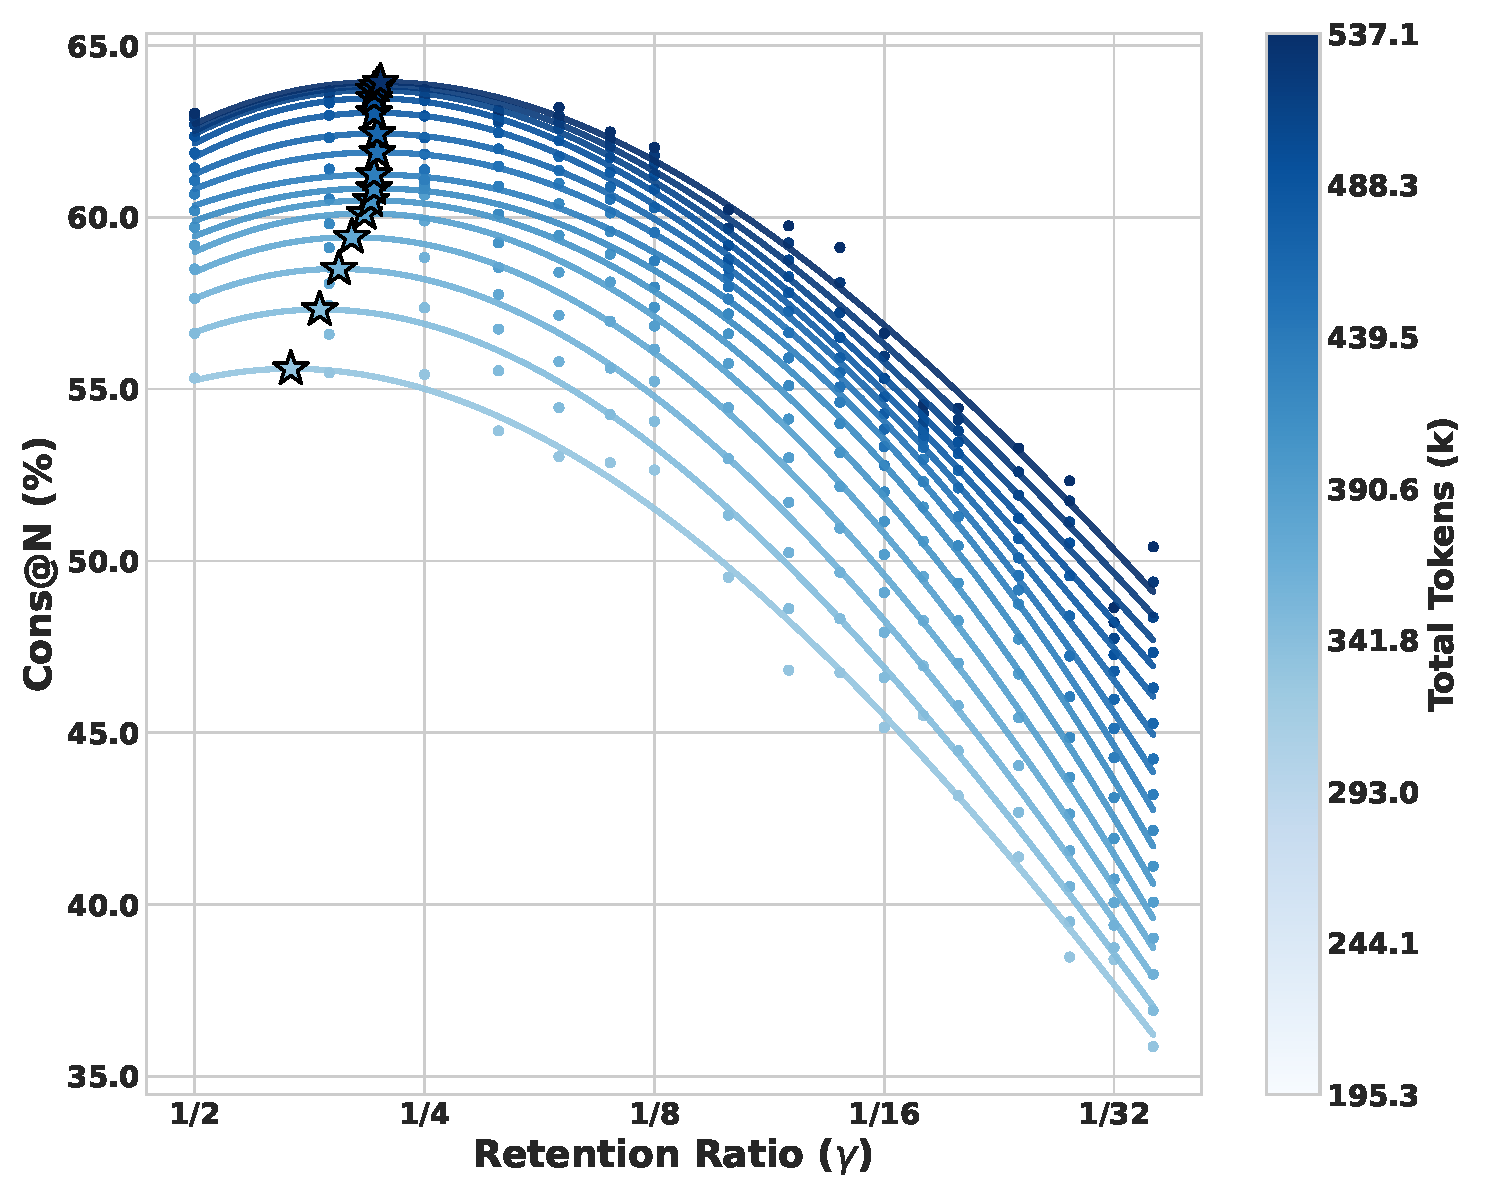
\includegraphics[width=\linewidth]{figures/Optimal_Pruning/1.5B_aime_2048_iso.pdf}
%     \caption{AIME ($L_p=2048$)}
%     \label{fig:ablation_math_2048}
%   \end{subfigure}
%   \hfill
%   \begin{subfigure}[b]{0.45\linewidth}
%     \centering
%     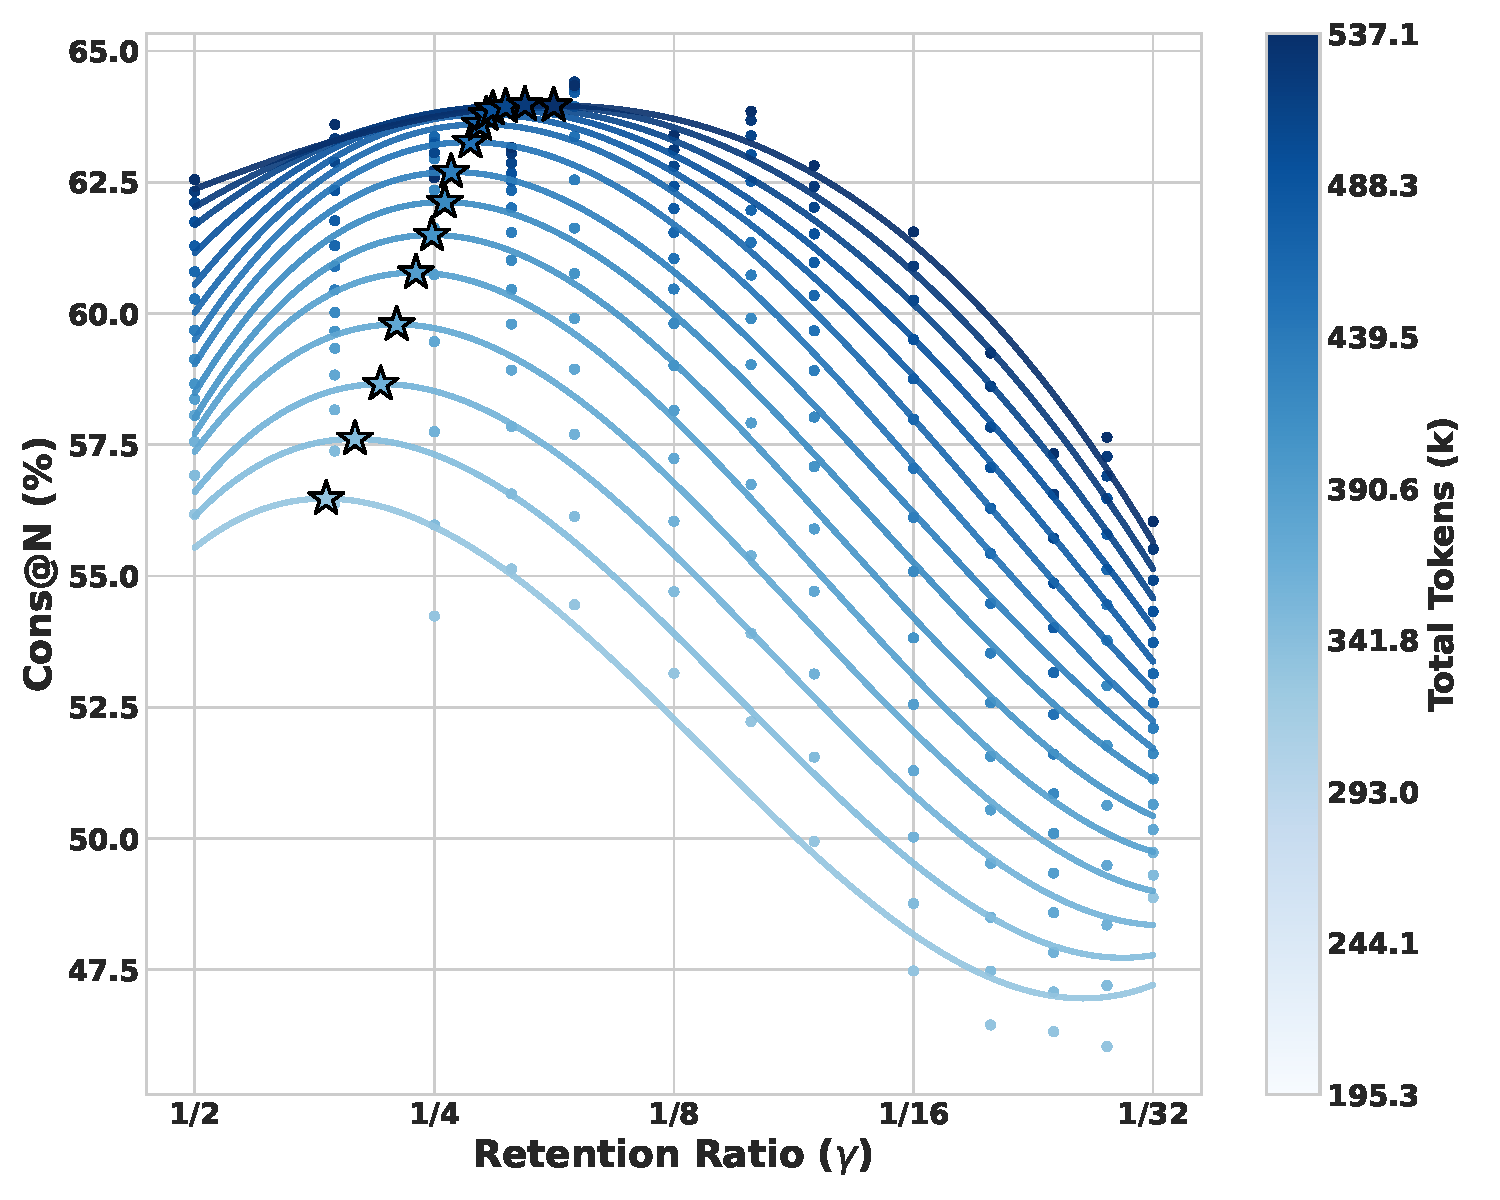
\includegraphics[width=\linewidth]{figures/Optimal_Pruning/1.5B_aime_4096_iso.pdf}
%     \caption{AIME ($L_p=4096$)}
%     \label{fig:ablation_math_4096}
%   \end{subfigure}
  
%   \vspace{1em}
%   % --- Row 2: GPQA Tasks ---
%   \begin{subfigure}[b]{0.45\linewidth}
%     \centering
%     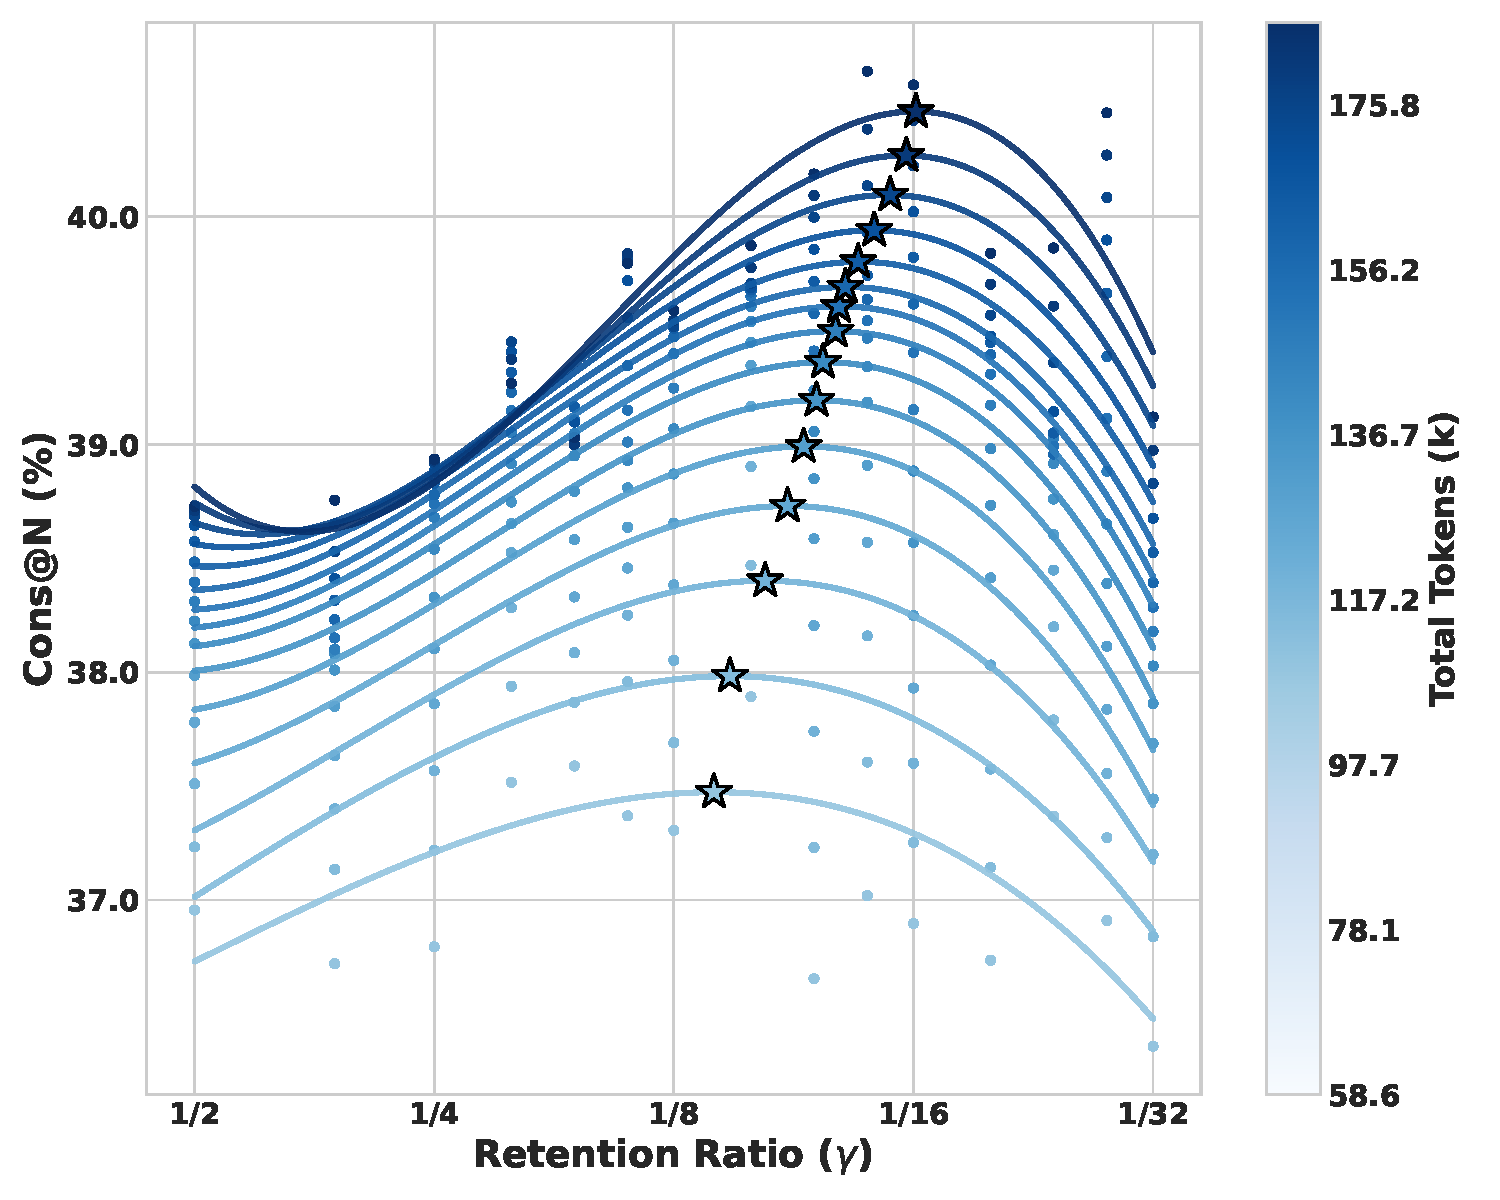
\includegraphics[width=\linewidth]{figures/Optimal_Pruning/1.5B_gpqa_512_iso.pdf}
%     \caption{GPQA ($L_p=512$)}
%     \label{fig:ablation_gpqa_512}
%   \end{subfigure}
%   \hfill
%   \begin{subfigure}[b]{0.45\linewidth}
%     \centering
%     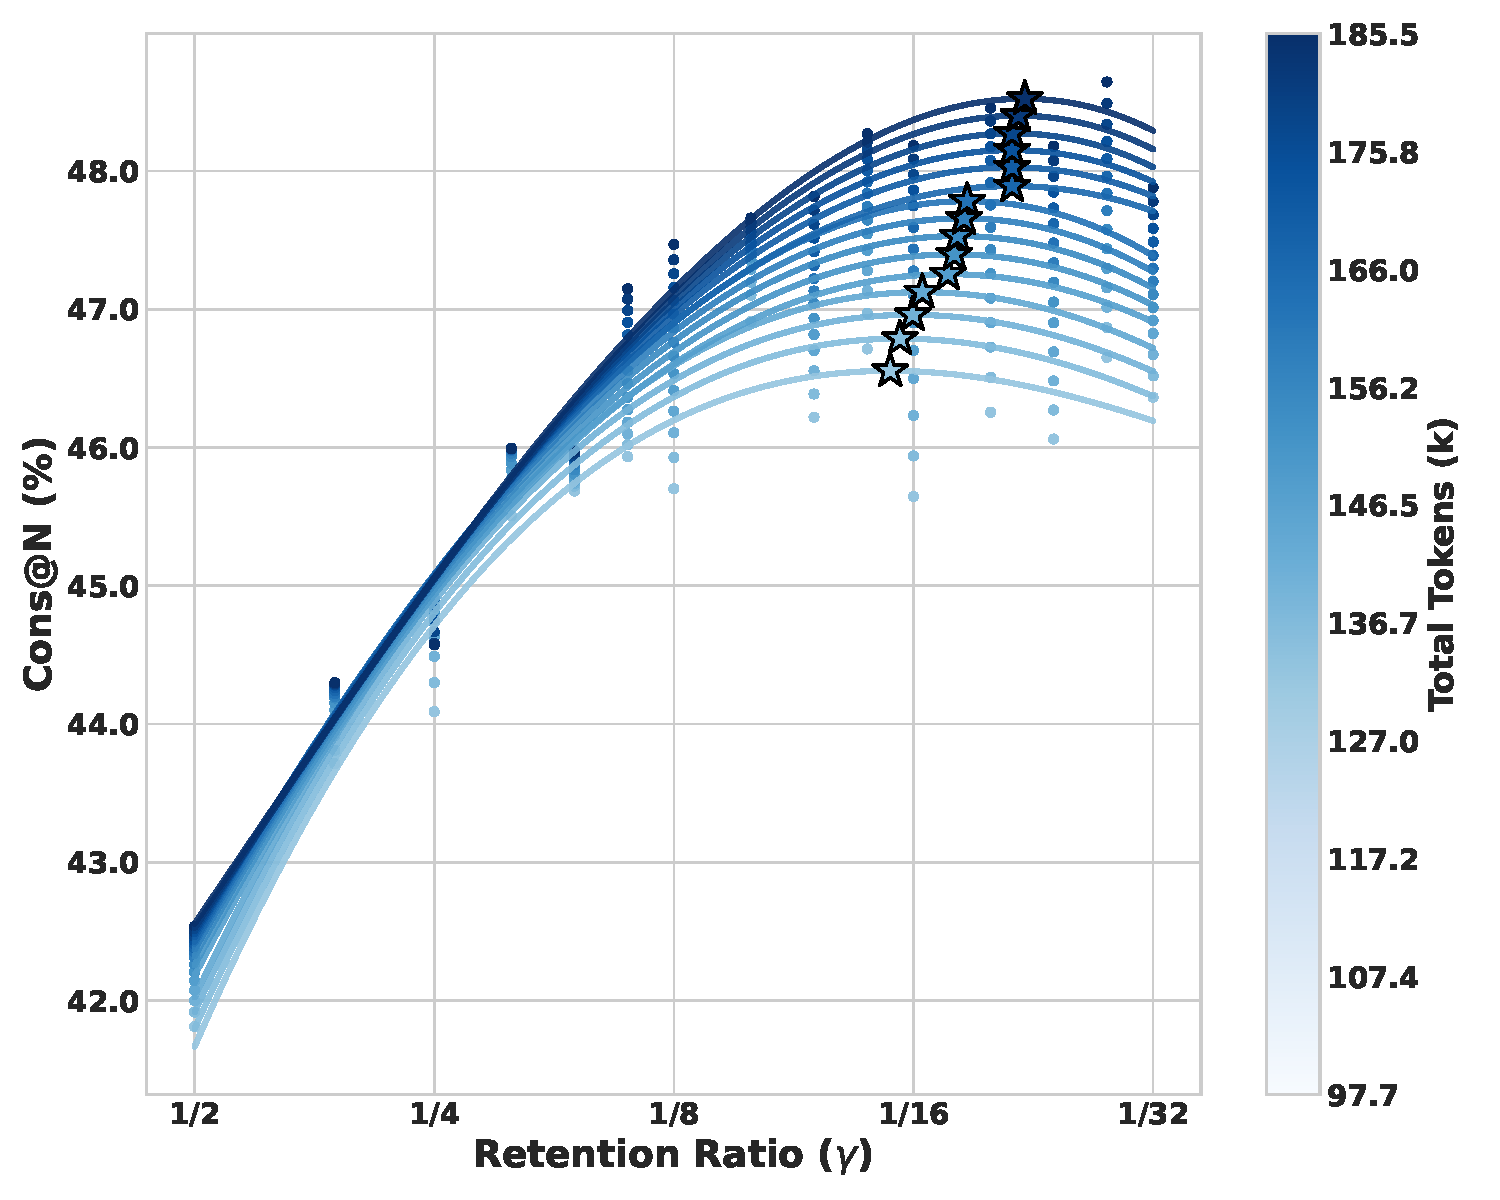
\includegraphics[width=\linewidth]{figures/Optimal_Pruning/1.5B_gpqa_1024_iso.pdf}
%     \caption{GPQA ($L_p=2048$)}
%     \label{fig:ablation_gpqa_2048}
%   \end{subfigure}

%   \caption{
%     \textbf{Performance comparison under different remaining ratios ($\gamma$) and prefix lengths ($L_p$).}
%     \textbf{Top Row (Math/AIME):} With shorter prefixes ($L_p=2048$), conservative pruning yields better performance, while longer prefixes ($L_p=4096$) improve robustness to aggressive pruning.
%     \textbf{Bottom Row (GPQA):} GPQA consistently benefits from aggressive remaining ratios, and increasing prefix length further stabilizes performance trends.
%   }
%   \label{fig:ablation_all_four}
% \end{figure*}

% \begin{figure*}[t] % 使用 figure* 使其跨越双栏
%   \centering
  
%   % --- Row 1: Math (AIME) Tasks ---
%   \begin{subfigure}[b]{0.32\linewidth}
%     \centering
%     \includegraphics[width=\linewidth]{figures/math_2048_poly_Cons_LogFit.pdf}
%     \caption{AIME ($L_p=2048$)}
%     \label{fig:ablation_math_2048}
%   \end{subfigure}
%   \hfill
%   \begin{subfigure}[b]{0.32\linewidth}
%     \centering
%     \includegraphics[width=\linewidth]{figures/math_3072_poly_Cons_LogFit.pdf}
%     \caption{AIME ($L_p=3072$)}
%     \label{fig:ablation_math_3072}
%   \end{subfigure}
%   \hfill
%   \begin{subfigure}[b]{0.32\linewidth}
%     \centering
%     \includegraphics[width=\linewidth]{figures/math_4096_poly_Cons_LogFit.pdf}
%     \caption{AIME ($L_p=4096$)}
%     \label{fig:ablation_math_4096}
%   \end{subfigure}
  
%   \vspace{1em} % 行间距
  
%   % --- Row 2: GPQA Tasks ---
%   \begin{subfigure}[b]{0.32\linewidth}
%     \centering
%     \includegraphics[width=\linewidth]{figures/gpqa_512_poly_Cons_LogFit.pdf}
%     \caption{GPQA ($L_p=512$)}
%     \label{fig:ablation_gpqa_512}
%   \end{subfigure}
%   \hfill
%   \begin{subfigure}[b]{0.32\linewidth}
%     \centering
%     \includegraphics[width=\linewidth]{figures/gpqa_1024_poly_Cons_LogFit.pdf}
%     \caption{GPQA ($L_p=1024$)}
%     \label{fig:ablation_gpqa_1024}
%   \end{subfigure}
%   \hfill
%   \begin{subfigure}[b]{0.32\linewidth}
%     \centering
%     \includegraphics[width=\linewidth]{figures/gpqa_2048_poly_Cons_LogFit.pdf}
%     \caption{GPQA ($L_p=2048$)}
%     \label{fig:ablation_gpqa_2048}
%   \end{subfigure}

%   \caption{
%     \textbf{Performance comparison under different remaining ratios ($\gamma$) and prefix lengths ($L_p$).} 
%     \textbf{Top Row (Math/AIME):} At shorter prefixes ($L_p=2048$), conservative pruning is preferred. As $L_p$ increases to 4096, the model becomes more robust to aggressive pruning.
%     \textbf{Bottom Row (GPQA):} This dataset consistently favors aggressive remaining ratios (e.g., 1/20, 1/32) regardless of prefix length, with longer prefixes further stabilizing performance.
%   }
%   \label{fig:ablation_all_six}
% \end{figure*}


\begin{figure*}[t]
\vspace{-12mm}
  \centering
  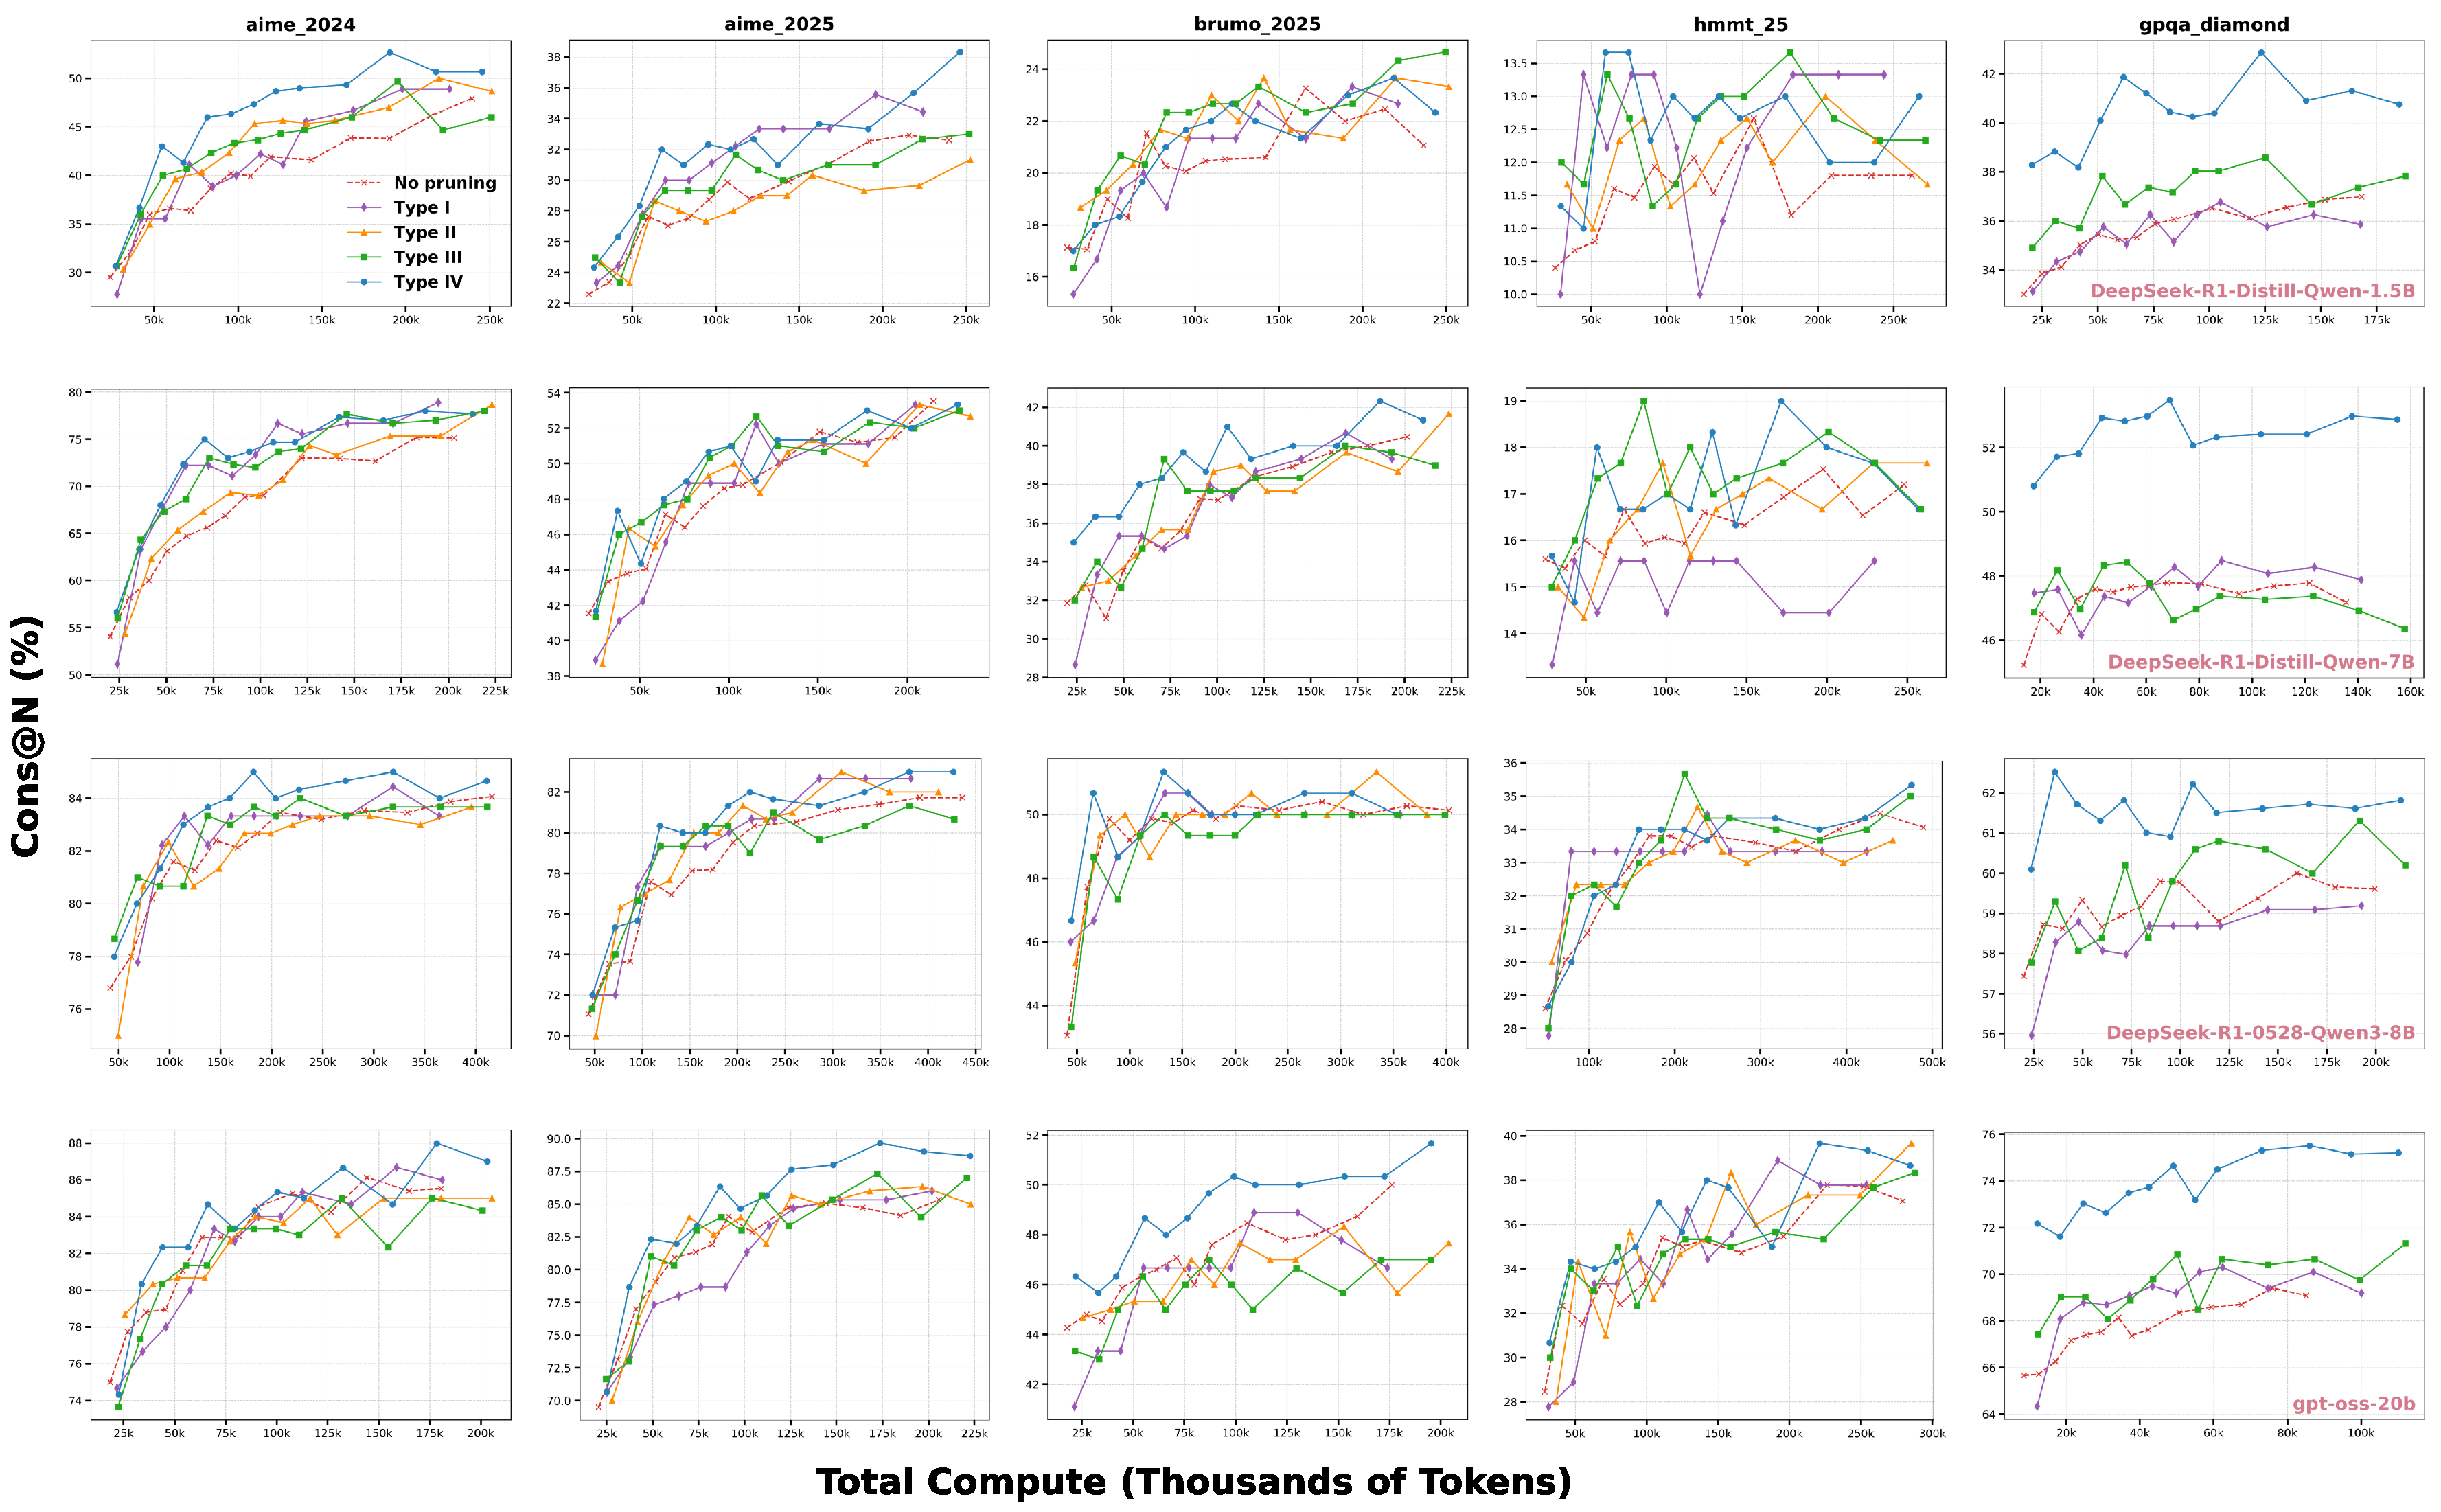
\includegraphics[width=\linewidth]{figures/scaling_main.pdf}
  \caption{
    Performance vs. compute for four types of $S$ on math and stem benchmarks.
    }
  \label{fig:scaling_main} 
\vspace{-4mm}
\end{figure*}

\section{A Closer Look at STOP}
\subsection{Determining the Optimal remaining ratios}
\label{subsec:Power-law}
% While the effectiveness of $S_\text{module}$ is validated, we still need to determine two critical hyperparameters: the prefix length ($L_\text{prefix}$) and the remaining ratio ($\gamma$).
% It is obvious that prefix longer -> the error is easier to find -> the effect much better.
% So the user can icrease the prefix length $L_\text{prefix}$ in their budget.
% However, the determination of the remaining ratio $\gamma$ is an obsticle.
% To give a clear guideline for $\gamma$ in practical settings, we first formalize this problem:

% Given a task with its reference length to solve it by the LRM $L_\text{task}$, the compute budget $C$ (tokens) and the prefix length $L_\text{prefix}$, our objective is to find a function $\gamma = f(C, L_\text{prefix}, L_\text{task})$ that maximizes the accuracy:
% \begin{equation}
%     \underset{f}{\arg \max} \text{ Accuracy}(C,L_\text{prefix},L_\text{task},\gamma)
% \end{equation}
% where $\gamma = f(C,L_\text{prefix},L_\text{task})$.
% If we can find a function $f$, we can use it as a guideline to predict optimal $\gamma$.

% To find $f$, we first apply $S_\text{module}$ to DS-1.5B, range the $\gamma$ from $\frac{1}{2}$ to $\frac{1}{32}$ on AIME 2024 and GPQA Diamond.
% We replicate the above experiments using four different $L_\text{prefix}$ and plot each with optimal points in Figure~\ref{fig:ablation_all_six}.
% Surprisingly, the optimal points in our results demonstrate consist and clear trends.
% (1) For certain $L_\text{prefix}$, incrase the compute budge $C$, the optimal $\gamma$ tends to decrease.
% (2) incease the $L_\text{prefix}$ and compute budge $C$, the trend of the optimal $\gamma$ tends to decrease.
% The two observations indicate that when we scale up the compute and prefix length, the error is more easier to identify, we can prune more paths to increase the accuracy.

% Build on the two insights, we model the $f$ as:

% \begin{equation}\small
%     \gamma^{-1} = f(C, L_{\text{prefix}}, L_{\text{task}}) = aC^b\frac{L_\text{prefix}^c}{L_\text{task}^d}
% \end{equation}\label{eq:optimial_gamma}
% % \begin{equation}\small
% % \begin{aligned}
% %     \gamma^{-1} = f(C, L_{\text{prefix}}, L_{\text{task}}) &\approx A \cdot \frac{C^a}{\mathcal{D}}, \\
% %     \quad \text{where} \quad \mathcal{D} &= \frac{L_{\text{task}}^{\delta}}{L_{\text{prefix}}^{\beta}}
% % \end{aligned}
% % \label{eq:optimial_gamma}
% % \end{equation}

% In this formulation, all input variables are normalized to units of 1024 tokens.
% After fitting, we obtain the global coefficients $a \approx 1.17 \times 10^4$, $b \approx 0.46$, $c \approx 0.40$, and $d \approx 4.55$.
% In Figure~\ref{fig:optimal_pruning_ratio_with_fit}, we can clearly see that our predicted curve fits the optimal point well.
% \paragraph{The optimization objective.}
While the effectiveness of 
Type~\ref{type:module} is established, optimal deployment requires precise tuning of two critical hyperparameters: the prefix length ($L_\text{prefix}$) and the retention ratio ($\gamma$).
Since increasing $L_\text{prefix}$ generally enhances error detection at the cost of higher latency, users typically fix this parameter according to their specific latency budget.
However, determining the optimal retention ratio $\gamma$ remains non-trivial.
To provide a practical guideline, we formalize the objective as finding a function $\gamma = f(C, L_\text{prefix}, L_\text{task})$ that maximizes accuracy given a compute budget $C$ (in tokens) and a reference task length $L_\text{task}$:
\begin{equation}\small
    \underset{f}{\arg \max} \text{ Accuracy}(C,L_\text{prefix},L_\text{task},\gamma),
\end{equation}
\vspace{-2mm}
where $\gamma$ determines the proportion of paths retained.
Identifying this function $f$ enables the prediction of the optimal $\gamma$ for any given configuration.

\paragraph{Consistent Empirical Trends across Various Settings}
To derive $f$, we conduct experiments using DS-Qwen-2.5-1.5B on AIME 2024 and GPQA Diamond, sweeping $\gamma$ from $1/32$ to $1/2$ across four distinct $L_\text{prefix}$ settings.
The results, plotted in Figure~\ref{fig:gamma_all_four}, exhibit consistent trends: the optimal $\gamma$ decreases as either the compute budget $C$ or the prefix length $L_\text{prefix}$ increases.
These observations indicate that with sufficient compute or richer context, the model identifies futile paths more reliably, thereby allowing for more aggressive pruning (lower $\gamma$) without compromising accuracy.

\paragraph{Formalizing Empirical Findings}
Building on these insights, we model the relationship using a power-law formulation:
\begin{equation}\small
    \gamma^{-1} = f(C, L_{\text{prefix}}, L_{\text{task}}) = aC^b\frac{L_\text{prefix}^c}{L_\text{task}^d}.
    \label{eq:optimial_gamma}
\end{equation}
In this formulation, all input variables are normalized to units of 1,024 tokens.
Fitting this model to our empirical data yields empirical coefficients $a \approx 1.17 \times 10^4$, $b \approx 0.46$, $c \approx 0.40$, and $d \approx 4.55$.
As illustrated in Figure~\ref{fig:optimal_pruning_ratio_with_fit}, the predicted curve aligns closely with the empirical optimal points, offering a robust guideline for parameter selection in practical deployments.

\paragraph{Applying the Empirical Guideline}
To facilitate practical deployment, we apply the derived guideline to predict the optimal retention ratio $\gamma$ for specific configurations without exhaustive search.
Specifically, for a task with a shorter response horizon ($L_{\text{task}} \approx 8{,}650$), a prefix length of $L_{\text{prefix}} = 2{,}048$, and a total compute budget of $C = 158\text{k}$ tokens, the scaling law predicts an optimal inverse retention ratio of $\gamma^{-1} \approx 9.63$, corresponding to $\gamma \approx 10\%$.
Conversely, for a task with a longer reasoning chain ($L_{\text{task}} \approx 12\text{k}$, $L_{\text{prefix}} = 3\text{k}$, and $C = 275\text{k}$), it yields a more conservative estimate of $\gamma^{-1} \approx 3.36$.

These predictions are consistent with our empirical observations, indicating that the scaling law naturally adapts to variations in task complexity.
For detailed lookup guidelines across a broader range of configurations, we refer readers to \textbf{Appendix~\ref{app:gamma_guidelines}}.




\begin{figure*}[ht]
\vspace{-12mm}
  \centering
  \begin{subfigure}[b]{0.24\linewidth}
    \centering
    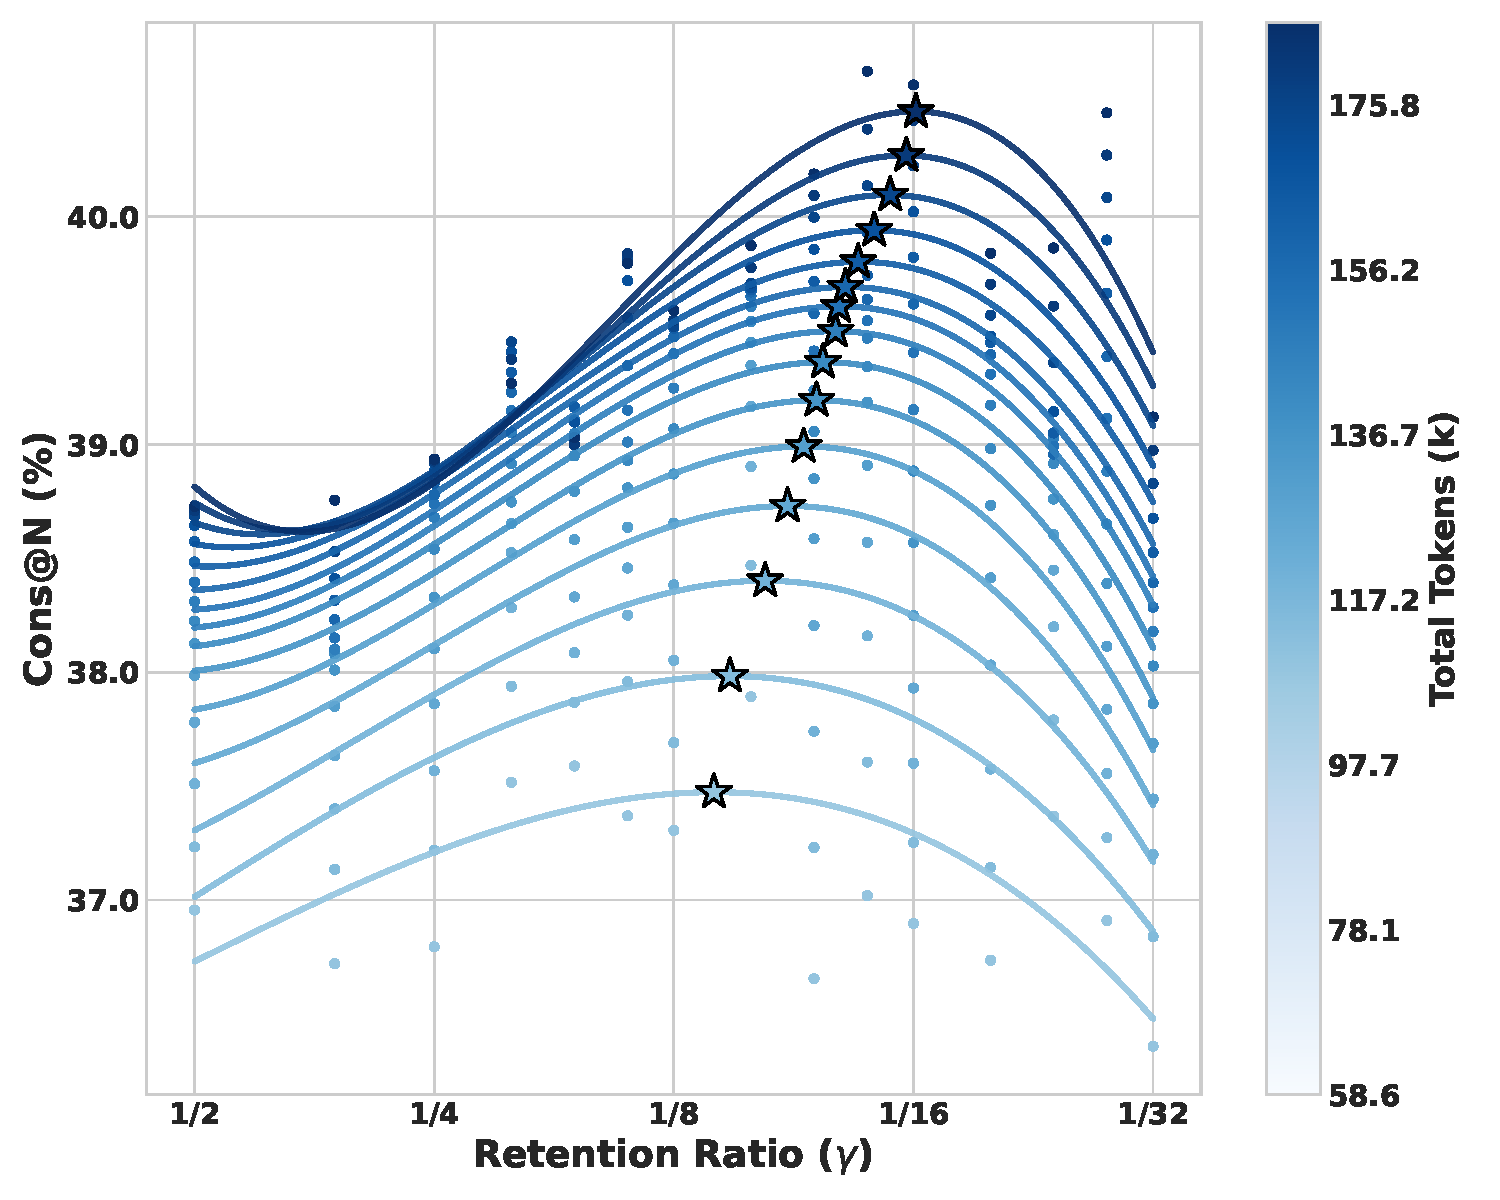
\includegraphics[width=\linewidth]{figures/Optimal_Pruning/1.5B_gpqa_512_iso.pdf}
    \caption{GPQA ($L_{\text{prefix}}=512$)}
  \end{subfigure}
  \hfill
  \begin{subfigure}[b]{0.24\linewidth}
    \centering
    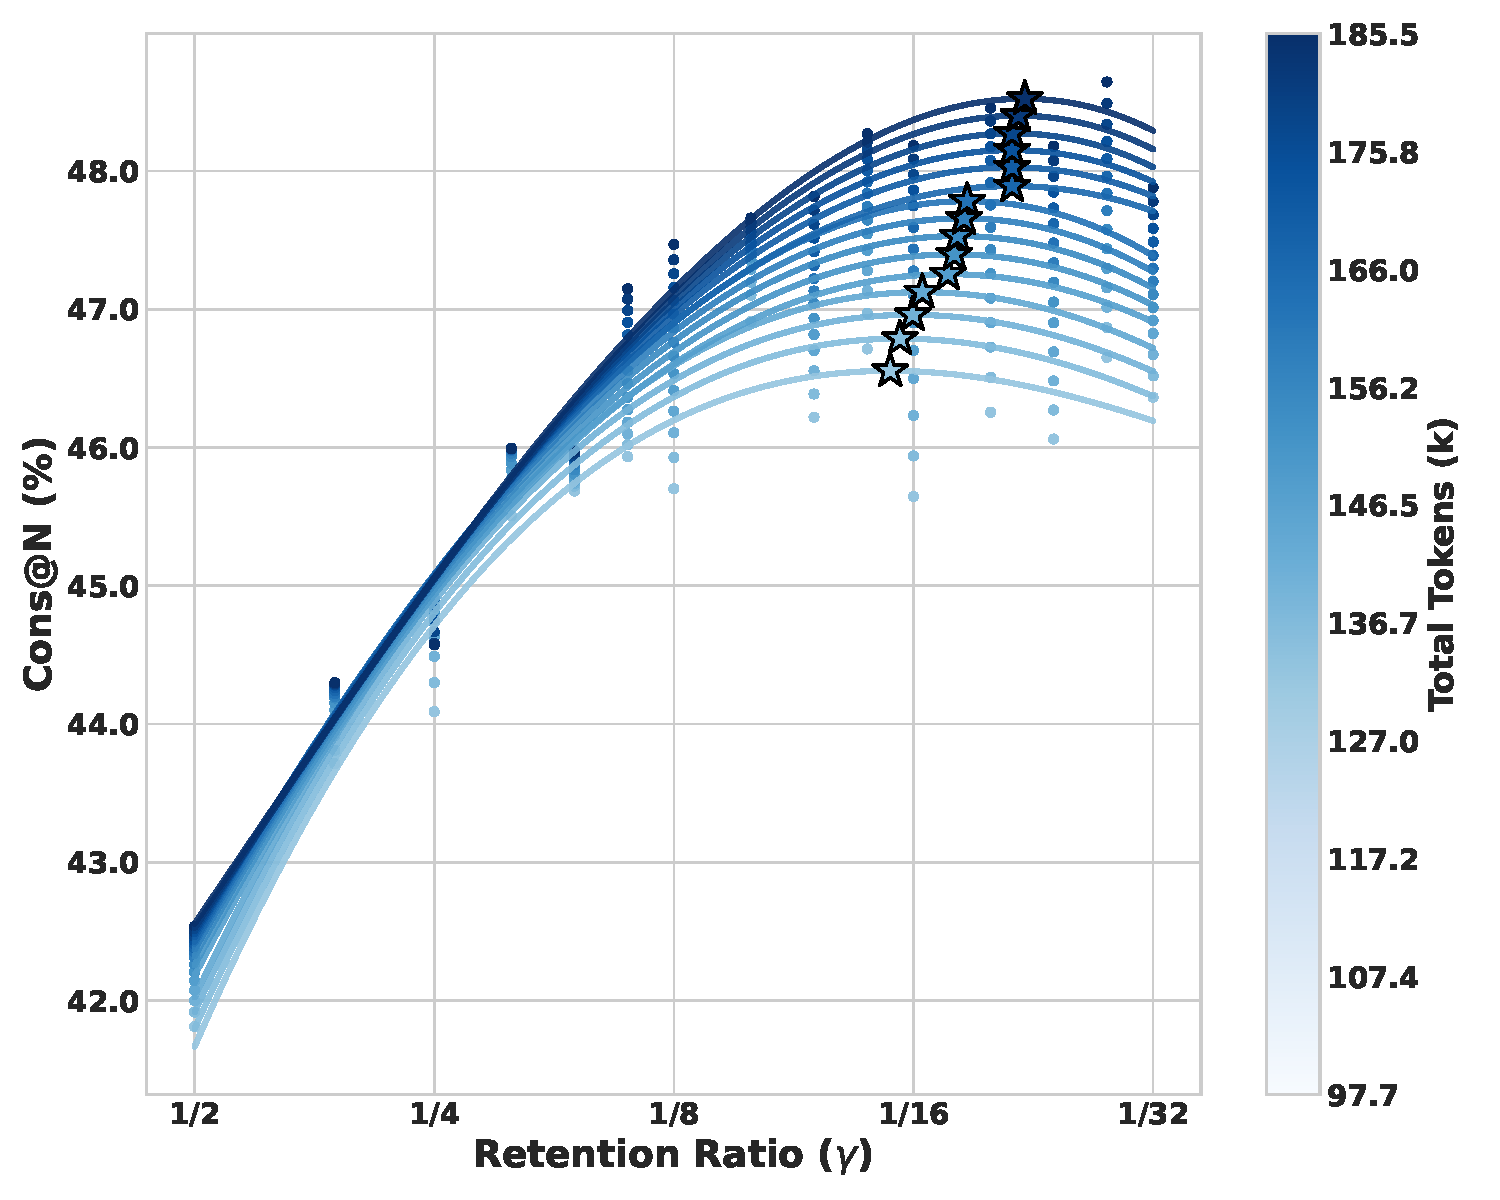
\includegraphics[width=\linewidth]{figures/Optimal_Pruning/1.5B_gpqa_1024_iso.pdf}
    \caption{GPQA ($L_{\text{prefix}}=1024$)}
  \end{subfigure}
  \hfill
  \begin{subfigure}[b]{0.24\linewidth}
    \centering
    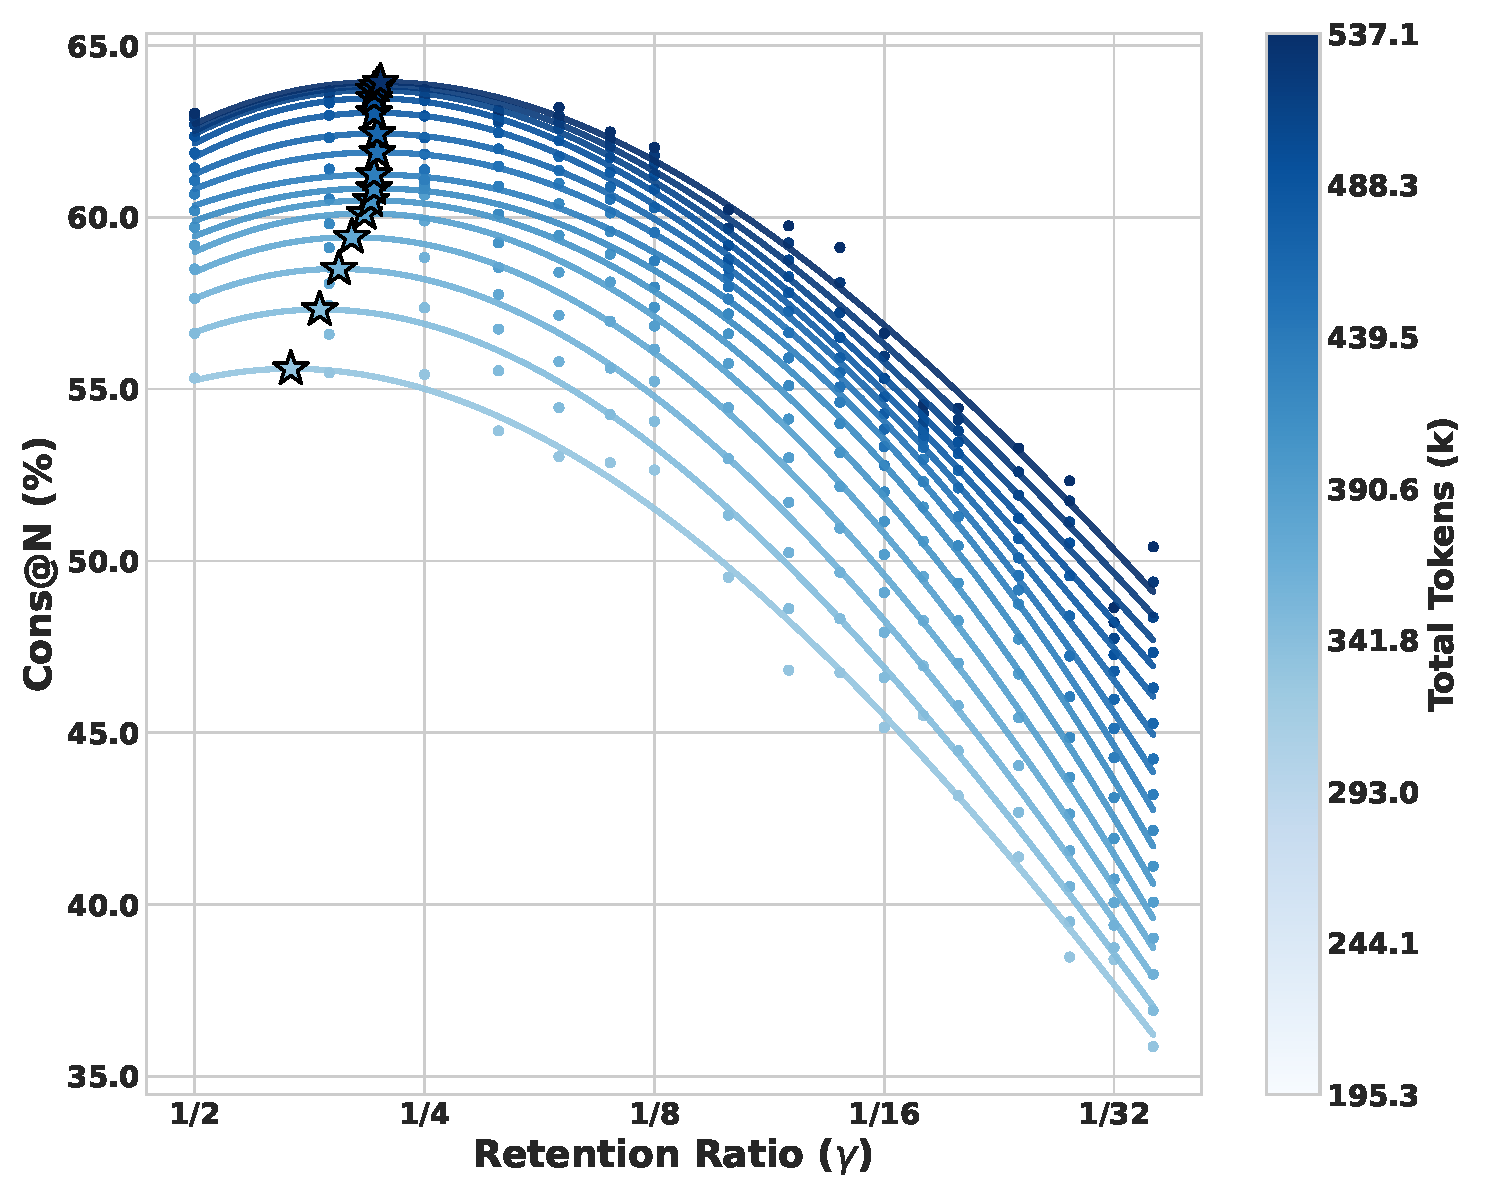
\includegraphics[width=\linewidth]{figures/Optimal_Pruning/1.5B_aime_2048_iso.pdf}
    \caption{AIME ($L_{\text{prefix}}=2048$)}
  \end{subfigure}
  \hfill
  \begin{subfigure}[b]{0.24\linewidth}
    \centering
    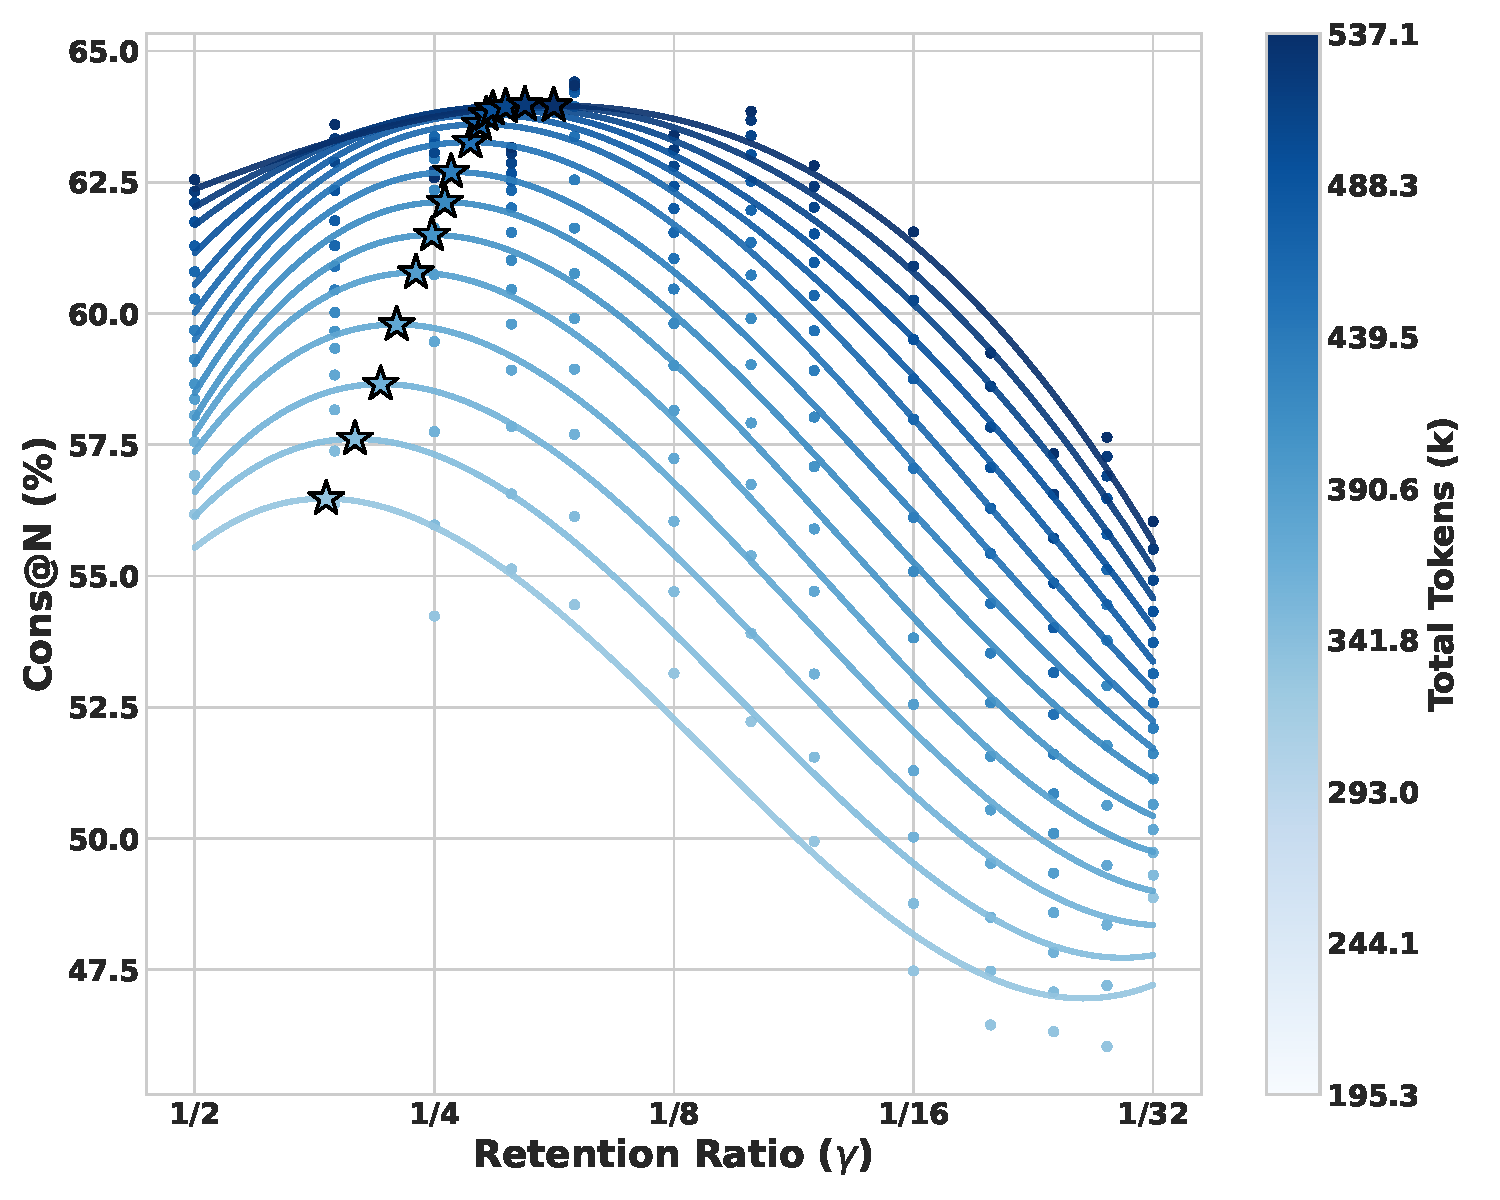
\includegraphics[width=\linewidth]{figures/Optimal_Pruning/1.5B_aime_4096_iso.pdf}
    \caption{AIME ($L_{\text{prefix}}=4096$)}
  \end{subfigure}
  \caption{
    Performance comparison under different retention ratios ($\gamma$) and prefix lengths ($L_{\text{prefix}}$).
    % AIME benefits from conservative pruning at shorter prefixes, while GPQA consistently favors aggressive pruning even at early stages. 
    % With extended $L_{\text{prefix}}$, both benchmarks effectively sustain performance under higher selectivity.
  }
  \label{fig:gamma_all_four}
\vspace{-4mm}
\end{figure*}

\begin{figure}[t]
  \centering
  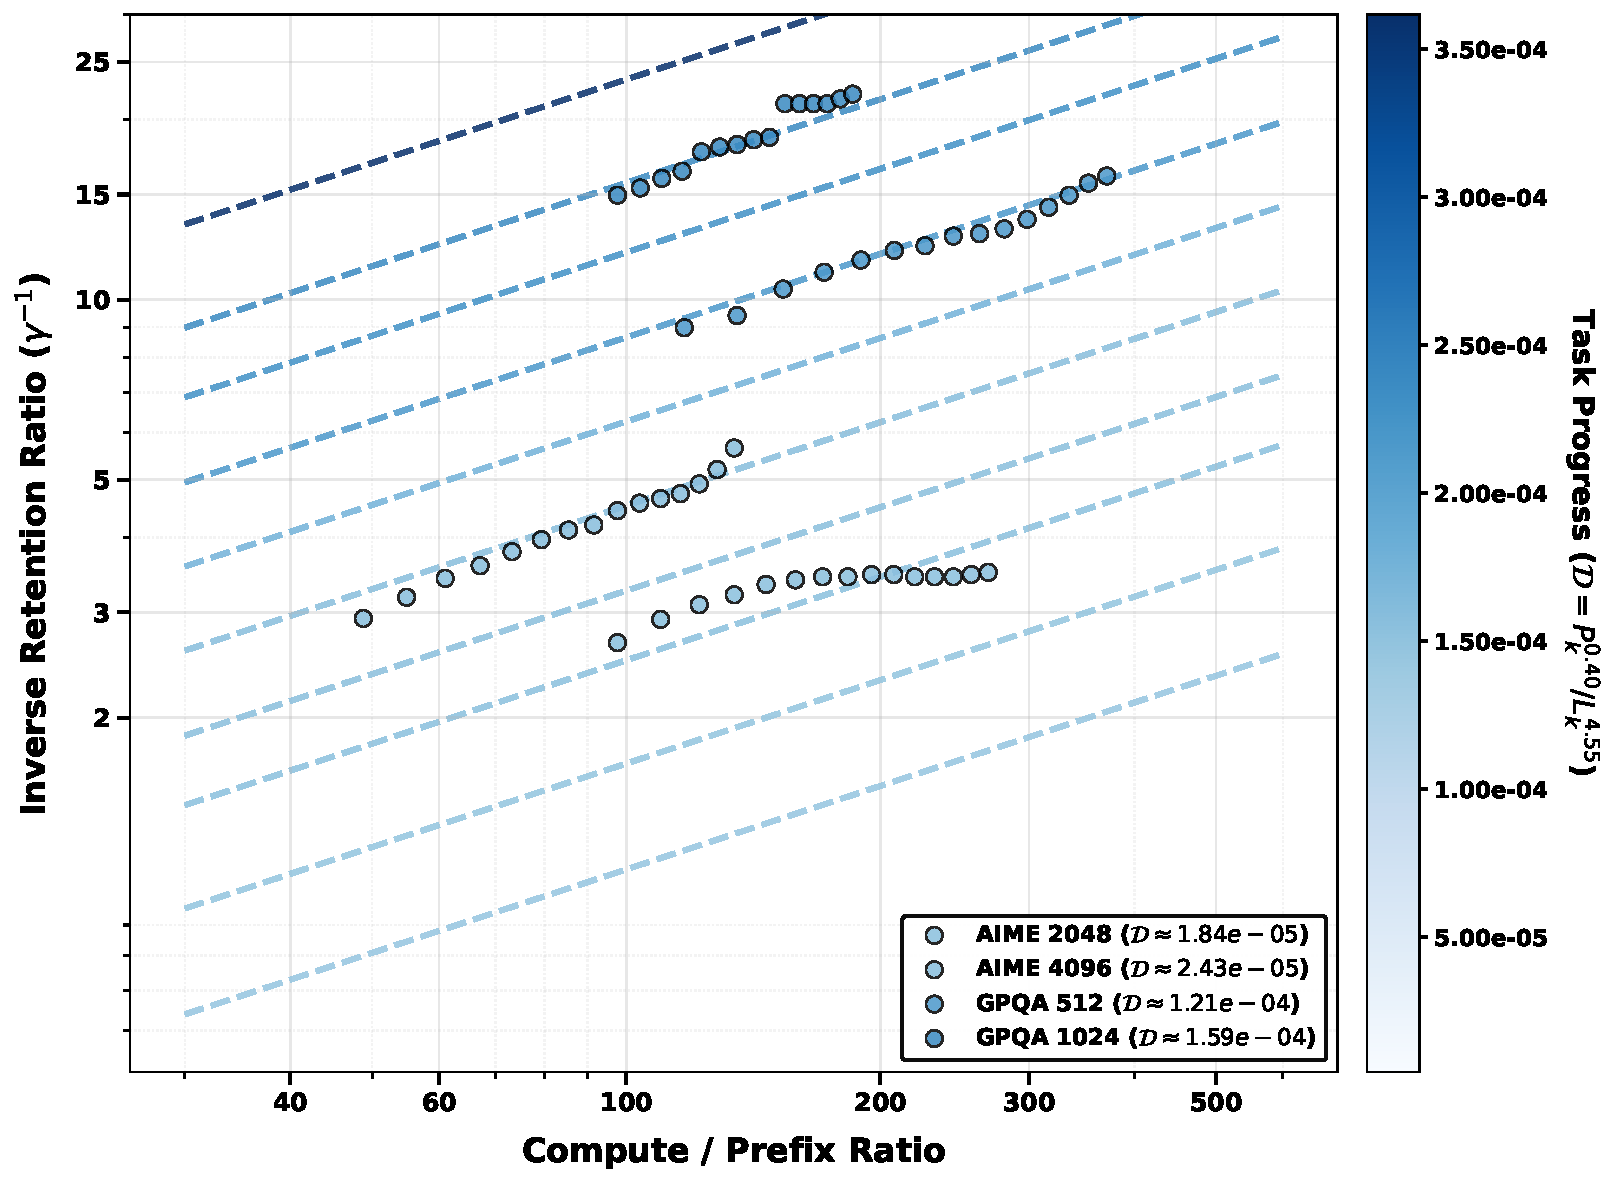
\includegraphics[width=\columnwidth]{figures/Optimal_Pruning/fitting.pdf}
\caption{
 Inverse retention ratio $\gamma^{-1}$ vs.\ compute-to-prefix ratio. The theoretical curves (Eq.~\ref{eq:optimial_gamma}) closely align with empirical observations across varying reasoning progress levels.
}\label{fig:optimal_pruning_ratio_with_fit}
\vspace{-4mm}
\end{figure}

\subsection{Ablations and Analysis}\label{subsec:ablation}
To validate the core design choices of \textbf{STOP}, we examine two critical dimensions: the quality of the supervision signal and the computational overhead during inference.


% \paragraph{Supervision Signal: Soft vs. Hard Labels.}
\paragraph{Ablation: Quality of the Supervision Signal}
\textbf{STOP} uses Monte Carlo (MC) estimation with $K=32$ samples to generate probabilistic soft labels ($s^{mc}$), and we compare this setting with binary hard-label supervision, which corresponds to a single-sample estimate ($K=1$). While hard labels are computationally cheap, they introduce high variance because prefix quality depends on a single stochastic continuation. As shown in Table~\ref{tab:ablation_supervision}, increasing the sampling budget from $K=1$ to $K=32$ consistently improves performance. On AIME 2024, soft supervision improves Cons@N from 46.67\% to 53.33\%. These results indicate that MC-based soft labels provide a low-variance signal that enables the lightweight \textbf{STOP} module to learn stable pruning boundaries.

\begin{table}[ht]
\centering

\caption{Performance comparison between hard labels ($K=1$) and MC-estimated soft labels ($K=32$).}
\label{tab:ablation_supervision}
\resizebox{0.9\linewidth}{!}{
\begin{tabular}{l l c c}
\toprule
\textbf{Dataset} & \textbf{Supervision Type} & \textbf{avg@8|64 (\%)} & \textbf{Cons@N (\%)} \\
\midrule
\multirow{2}{*}{AIME 24} & Hard Labels ($K=1$) & 35.42 & 46.67 \\
 & \textbf{Soft Labels ($K=32$)} & \textbf{36.67} & \textbf{53.33} \\
\midrule
\multirow{2}{*}{GPQA} & Hard Labels ($K=1$) & 40.78 & 47.98 \\
 & \textbf{Soft Labels ($K=32$)} & \textbf{41.73} & \textbf{48.48} \\
\bottomrule
\end{tabular}
}
\vspace{-4mm}
\end{table}

\begin{findings}
% Soft labels are essential for stable training. % context 不够
When training pruning method, soft labels (0.0 to 1.0) have lower variance than hard labels (0 or 1).
\end{findings}

\paragraph{Ablation: Necessity of Critique Adapter}
Given that the LRM's internal states already encode rich reasoning history, a natural question arises: Is a simple linear classifier sufficient to decode the pruning signal?
As shown in Table~\ref{tab:ablation_lora}, the answer is negative. Removing the LoRA adapter leads to a significant performance drop (e.g., from \textbf{36.67\%} to \textbf{31.67\%} on AIME 2024).
This phenomenon highlights a fundamental misalignment: the LRM's native representations are optimized for predicting next token, not value discrimination.
A linear head alone struggles to extract quality assessments from this generation-centric feature space.

\begin{table}[ht]
\centering
\caption{Comparing the STOP module with a simple linear classifier confirms that raw internal states require adaptation to perform effective self-evaluation.}
\label{tab:ablation_lora}
\resizebox{0.9\linewidth}{!}{
\begin{tabular}{l l c c}
\toprule
\textbf{Dataset} & \textbf{Configuration} & \textbf{avg@8|64 (\%)} & \textbf{Cons@N (\%)} \\
\midrule
\multirow{2}{*}{AIME 24} & STOP w/o Adapter & 31.67 & 46.67 \\ 
 & \textbf{STOP} & \textbf{36.67} & \textbf{53.33} \\ 
\midrule
\multirow{2}{*}{GPQA} & STOP w/o Adapter & 33.96 & 35.35 \\ 
 & \textbf{STOP} & \textbf{41.73} & \textbf{48.48} \\ 
\bottomrule
\end{tabular}
}
\vspace{-4mm}
\end{table}

\begin{findings}
High-quality self-correction cannot be achieved by merely probing the states in LRMs; it requires a specialized transformation to bridge the gap between thinking forward (generation) and looking back (reflection).
\end{findings}

\paragraph{Ablation: Sensitivity to Design Choices}
We further examine the sensitivity of \textbf{STOP} to key design choices, namely the number of \texttt{[STOP]} tokens and the LoRA rank. As shown in Table~\ref{tab:ablation_stop_tokens}, performance improves with more tokens, peaks at 4--6, and then degrades with further increases, indicating a trade-off between expressive capacity and overfitting. Similarly, Table~\ref{tab:ablation_rank} shows that moderate ranks (e.g., $r=128$) achieve the best performance, while larger ranks lead to slight degradation, suggesting that excessive capacity is unnecessary.

\begin{findings}
STOP is robust to reasonable hyperparameter choices and does not require large adapters to perform effectively.
\end{findings}

\begin{table}[ht]
\centering
\caption{Effect of the number of \texttt{[STOP]} tokens (DS-Qwen-2.5-1.5B, AIME 2024, $L_{\text{prefix}}=2048$).}
\label{tab:ablation_stop_tokens}
\resizebox{0.6\linewidth}{!}{
\setlength{\tabcolsep}{4pt}
\begin{tabular}{c c | c c}
\toprule
\# Tokens & avg@32$|$256 & \# Tokens & avg@32$|$256 \\
\midrule
1 & 30.10 & 6 & \textbf{37.71} \\
2 & 33.54 & 7 & 36.15 \\
3 & 35.94 & 8 & 35.00 \\
4 & 36.86 & 9 & 33.65 \\
5 & 36.77 & - & - \\
\bottomrule
\end{tabular}
}
\vspace{-5mm}
\end{table}

\begin{table}[ht]
\vspace{-2mm}
\centering
\caption{Effect of LoRA rank (DS-Qwen-2.5-1.5B, AIME 2024).}
\label{tab:ablation_rank}
\resizebox{0.5\linewidth}{!}{
\setlength{\tabcolsep}{4pt}
\begin{tabular}{c c c}
\toprule
Rank & Params (M) & avg@8$|$64 \\
\midrule
32  & 36.9  & 32.50 \\
64  & 73.9  & 36.25 \\
\textbf{128} & \textbf{147.7} & \textbf{36.67} \\
256 & 295.4 & 35.83 \\
\bottomrule
\end{tabular}
}
\vspace{-5mm}
\end{table}

\paragraph{Analysis: Computational Overhead}
We quantify the inference latency on a single NVIDIA H100 GPU using DS-Qwen-2.5-7B with a fixed prefix length of $2,048$.
As detailed in Table~\ref{tab:latency}, existing paradigms incur notable costs: Type~\ref{type:aux} requires full sequence re-encoding, resulting in the highest latency (\textbf{1.13\,s}, 3.37\% overhead), while Type~\ref{type:heuristic} suffers from the computational bottleneck of pairwise similarity calculations (\textbf{0.38\,s}).
In stark contrast, \textbf{STOP} (Type~\ref{type:module}) minimizes overhead to a negligible \textbf{0.20\,s} (\textbf{0.59\%}).
This efficiency stems directly from our architectural design: by \textbf{reusing the pre-computed KV cache} and restricting verification to a single forward pass of special tokens, STOP eliminates redundant computation, ensuring high-throughput deployment.

\begin{table}[ht]
\centering
\caption{Inference overhead analysis. STOP achieves near-zero cost by avoiding re-encoding.}
\label{tab:latency}
\resizebox{0.85\linewidth}{!}{
\begin{tabular}{l c c}
\toprule
\textbf{Pruning Paradigm} & \textbf{Latency / Check} & \textbf{Relative Overhead} \\
\midrule
Type~\ref{type:aux} & 1.13\,s & 3.37\% \\
Type~\ref{type:heuristic} & 0.38\,s & 0.93\% \\
\rowcolor{gray!10} \textbf{Type~\ref{type:module} (STOP)} & \textbf{0.20\,s} & \textbf{0.59\%} \\
\bottomrule
\end{tabular}
}
\vspace{-4mm}
\end{table}


\paragraph{Analysis: Generalization to Non-Math/STEM Tasks}
To assess whether \textbf{STOP} captures universal reasoning patterns beyond mathematics and science, we extend our evaluation to \textbf{ZebraLogic}, a benchmark designed to evaluate combinatorial reasoning and constraint satisfaction capabilities through logic grid puzzles.
Specifically, we conduct experiments on the multiple-choice mode (\texttt{mc\_mode}) to test reasoning under constraints.
Using the \textbf{DS-Qwen-2.5-7B} model, we evaluate 500 randomly sampled instances of moderate difficulty (Rows, Cols $\le 4$).
As shown in Table~\ref{tab:ablation_zebra}, \textbf{STOP} improves accuracy from 73.73\% to \textbf{77.23\%}.
This consistent gain confirms that the pruning signals learned by the module are not strictly domain-dependent, but rather transferable to general logical inference tasks.

\begin{table}[t]
\centering
\caption{\textbf{Generalization on ZebraLogic.} \textbf{STOP} \textbf{robustly generalizes} beyond math and science tasks.}
\label{tab:ablation_zebra}
\resizebox{0.9\linewidth}{!}{
\begin{tabular}{l c c c}
\toprule
\multirow{2}{*}{\textbf{Model}} & \textbf{No pruning (Baseline)} & \textbf{\textbf{STOP}} & \multirow{2}{*}{\textbf{Gain}} \\
\cmidrule(lr){2-2} \cmidrule(lr){3-3} % 这里改成了两段独立的横线，中间会自动断开
 & \textbf{avg@64 (\%)} & \textbf{avg@8|64 (\%)} & \\
\midrule
DS-Qwen-2.5-7B & 73.73 & \textbf{77.23} & \textbf{+3.50\%} \\
\bottomrule
\end{tabular}
}
\vspace{-3mm}
\end{table}

% \paragraph{Analysis: Generalization to Tool Use}
% Beyond static reasoning benchmarks, we further evaluate whether \textbf{STOP} generalizes to settings involving tool use.
% We consider the AIMO3 benchmark with tool integration, where the model is allowed to invoke external tools during reasoning.
% Using the \textbf{GPT-OSS-20B} model, we observe consistent improvements over the baseline (Table~\ref{tab:ablation_tool}), with avg@32 increasing from 54.38 to \textbf{58.75}.
% This result suggests that the pruning signal learned by \textbf{STOP} remains effective even when reasoning is interleaved with external tool interactions.
\paragraph{Analysis: Generalization to Tool Use}
We further evaluate whether \textbf{STOP} generalizes to realistic tool-use scenarios by submitting our system to the \textbf{AIMO3} competition, where models solve mathematical problems with access to external tools under a fixed evaluation protocol. Built on a \textbf{GPT-OSS-120B + tool} framework, we compare against a baseline that directly performs parallel reasoning without pruning under the same resource constraints; due to the competition setting (single H100 GPU and a 5-hour limit for 50 problems), the baseline cannot scale to larger sampling budgets. As shown in Table~\ref{tab:ablation_tool}, both STOP configurations consistently outperform the baseline, improving the score from \textbf{39} to \textbf{42} (24$\rightarrow$8) and \textbf{43} (16$\rightarrow$8), with the best configuration reaching \textbf{silver-level performance} on the public leaderboard, demonstrating that \textbf{STOP} remains effective in tool-augmented reasoning and translates into tangible gains in real-world competitive settings.


% \begin{table}[h]
% \centering
% \caption{Generalization to tool use on AIMO3 (GPT-OSS-20B with tool integration).}
% \label{tab:ablation_tool}
% \resizebox{0.75\linewidth}{!}{
% \begin{tabular}{c c | c c}
% \toprule
% \multicolumn{2}{c|}{Baseline + Tool} & \multicolumn{2}{c}{STOP + Tool} \\
% \cmidrule(lr){1-2} \cmidrule(lr){3-4}
% Avg@32 & Cons@32 & Avg@8$|$32 & Cons@8$|$32 \\
% \midrule
% 54.38 & 0.70 & \textbf{58.75} & \textbf{0.80} \\
% \bottomrule
% \end{tabular}
% }
% \vspace{-5mm}
% \end{table}



% \begin{findings}
% \textbf{ Cross-Domain Generalization.}
% \textbf{STOP} effectively generalizes to \textbf{logic puzzles}, indicating that it learns to identify \textbf{structural reasoning validity} rather than relying solely on domain-specific memorization.
% \end{findings}

\begin{table}[h]
\centering
\small
\setlength{\tabcolsep}{5pt}
\caption{Results on the AIMO3 competition setting with tool use (GPT-OSS-120B).}
\label{tab:ablation_tool}
\begin{tabular}{l c}
\toprule
\textbf{Method} & \textbf{Score} \\
\midrule
Baseline + Tool & 39 \\
STOP (24$\rightarrow$8) & 42 \\
STOP (16$\rightarrow$8) & \textbf{43} \\
\bottomrule
\end{tabular}
\vspace{-3mm}
\end{table}

\subsection{How STOP Attends}
\label{subsec:interpretability}
To understand how \textbf{STOP} distinguishes valid reasoning trajectories, we visualize the attention distribution of the \texttt{[STOP]} token (Figure~\ref{fig:attention_analysis}).
Overall, the module exhibits a broad attention pattern. It consistently attends to \textbf{multiple-choice options} (A, B, C, D) as well as discourse markers (e.g., ``Hmm'', ``Wait''), which enables it to track the structural progression of the reasoning process.

\paragraph{Process-oriented Evaluation}
Importantly, high-scoring and low-scoring trajectories present clearly distinct attention signatures.
In the \textbf{high-score case} (Figure~\ref{fig:attention_analysis}a), attention prioritizes the reasoning process rather than the final outcome.
Specifically, the \texttt{[STOP]} token focuses on \textbf{cognitive pivots} (e.g., the negation ``don't''), indicating an emphasis on logical operations that trigger self-correction.
In contrast, the \textbf{low-score case} (Figure~\ref{fig:attention_analysis}b) demonstrates a pattern of \textbf{premature closure}: attention shifts early to the terminal token (e.g., ``B'') while critical logical markers receive little attention.
Consequently, \textbf{STOP} penalizes such trajectories and interprets the lack of attention to logical pivots as evidence of reasoning failure.
See Appendix~\ref{app:mechanistic_interpretability} for more cases.

\begin{figure*}[t]
\vspace{-14mm}
  \centering
  \begin{subfigure}[b]{0.48\linewidth}
    \centering
    % 强制设定高度为 5.0cm 以保证左右对齐
    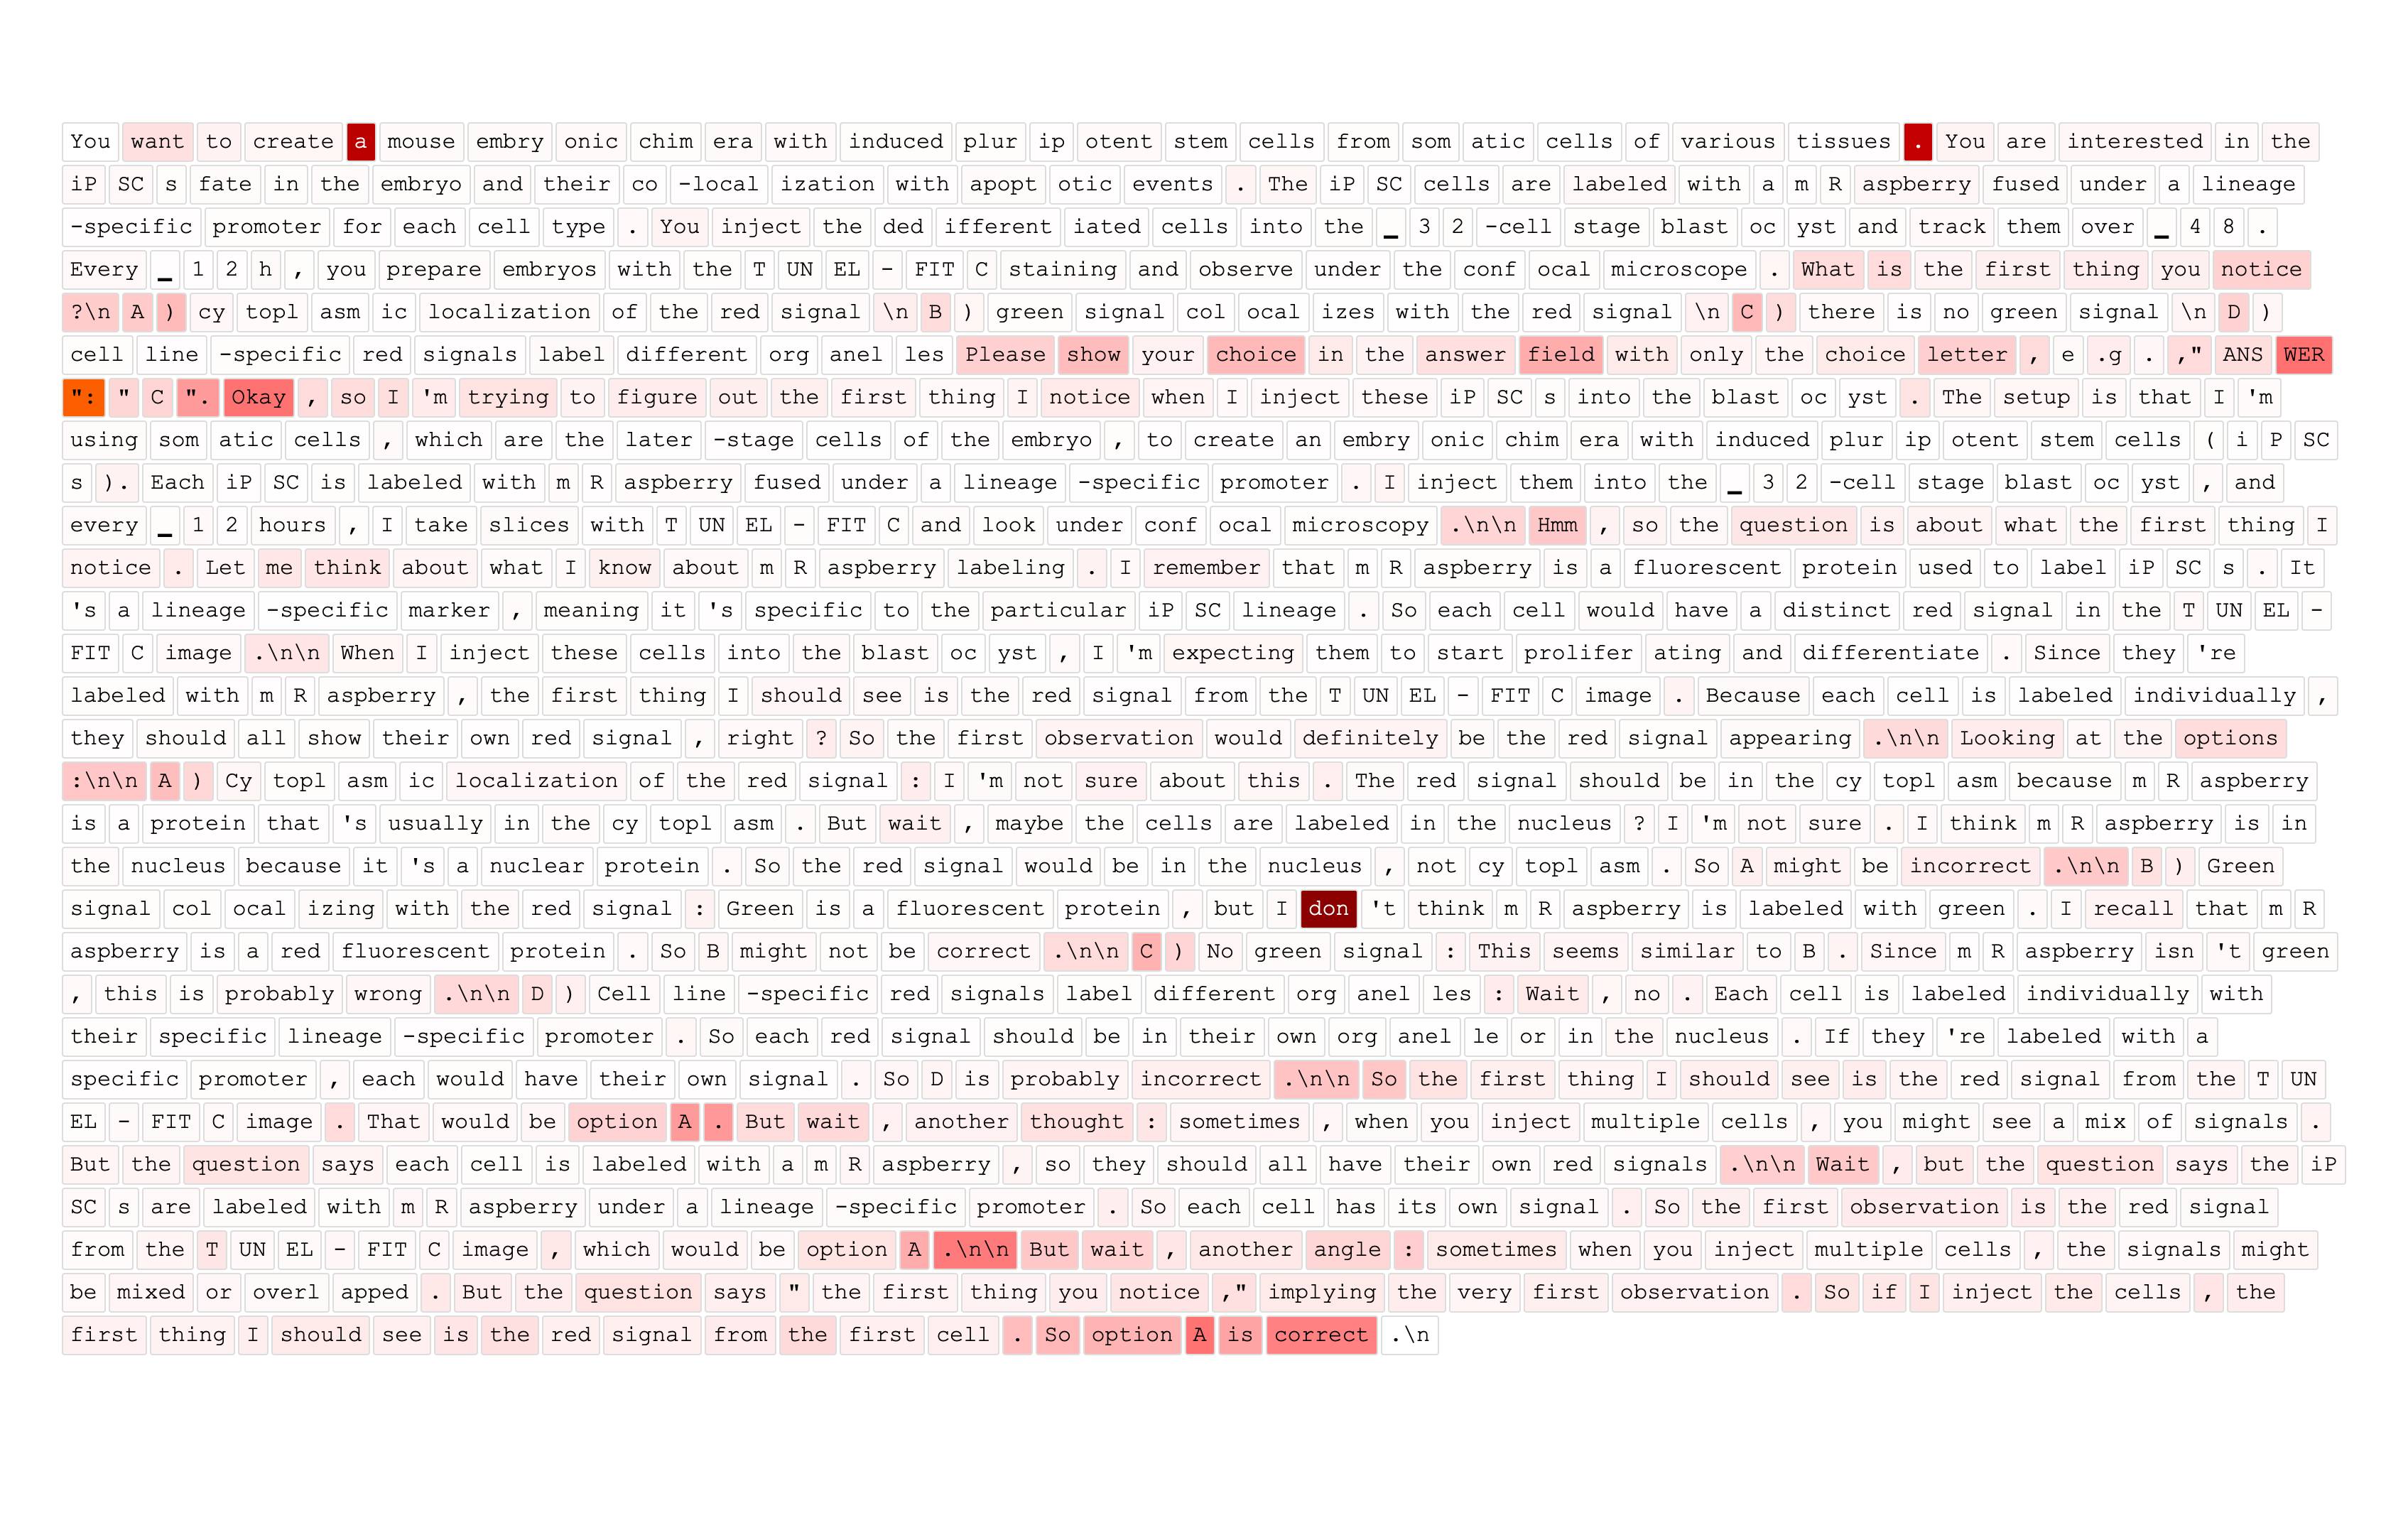
\includegraphics[height=5.0cm, keepaspectratio]{figures/high_case4.png}
    \caption{\textbf{High-scoring Path}}
    \label{fig:attn_correct}
  \end{subfigure}
  \hfill
  \begin{subfigure}[b]{0.48\linewidth}
    \centering
    % 强制设定高度为 5.0cm 以保证左右对齐
    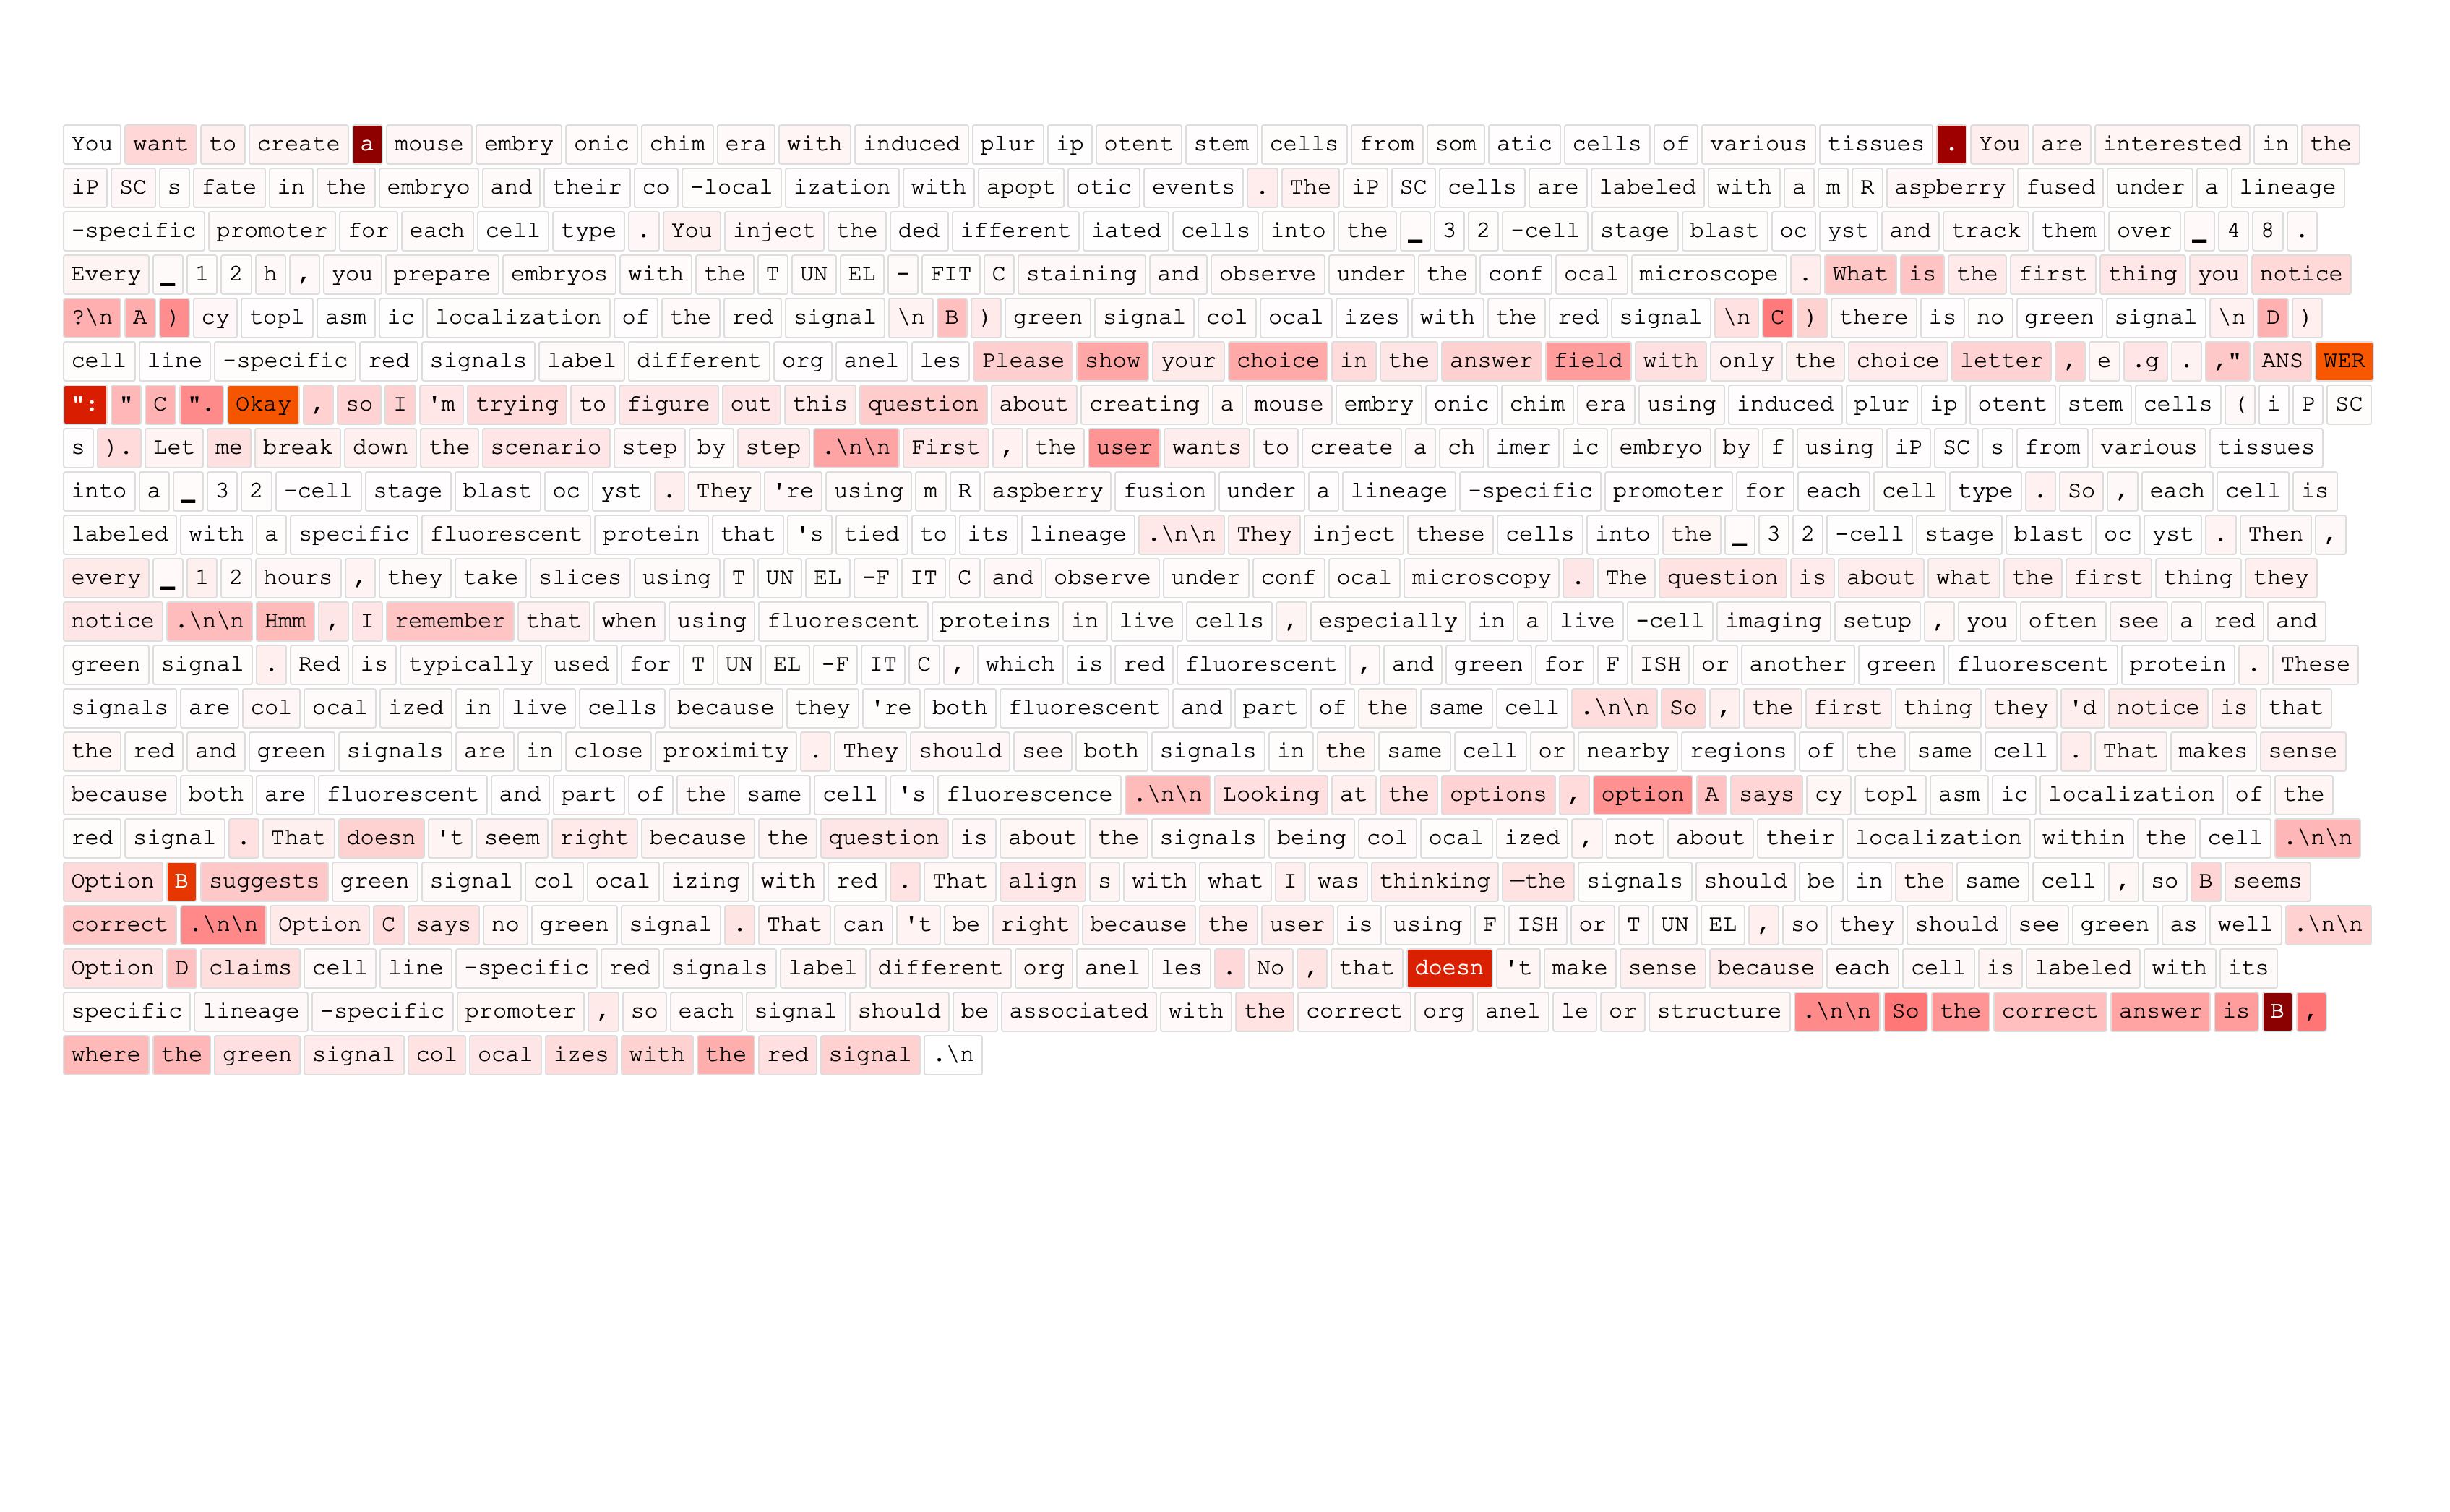
\includegraphics[height=5.0cm, keepaspectratio]{figures/low_case5.png} 
    \caption{\textbf{Low-scoring Path}}
    \label{fig:attn_incorrect}
  \end{subfigure}
  \vspace{-4mm}
\caption{\textbf{Attention Analysis of \texttt{[STOP]} Decision-Making.} High-scoring paths prioritize logical pivots (e.g., self-correction markers), whereas low-scoring paths fixate on terminal answer tokens. This contrast confirms that \textbf{STOP} functions as a process-oriented evaluator, rewarding reasoning integrity over premature closure.}
\label{fig:attention_analysis}
  \vspace{-5.0mm}
\end{figure*}


% \textbf{Finding 6: Process-Oriented Evaluation.}
% \textbf{STOP} acts as a \textbf{process-oriented evaluator}. It distinguishes reasoning quality by emphasizing \textbf{cognitive pivots} and penalizing \textbf{premature closure}.


% \begin{findings}
% \textbf{STOP} evaluates reasoning integrity by prioritizing logical pivots over premature closure.
% \end{findings}



% To understand the decision-making mechanism of STOP, we analyze the attention distribution of the \texttt{[STOP]} token, as shown in Figure~\ref{fig:attention_map}.

% We observe that the STOP module maintains a broad attention baseline across both trajectories.
% It consistently attends to the multiple-choice options (A, B, C, D) in the prompt and tracks discourse markers in the response (e.g., ``Hmm'', ``Wait'', ``So'', ``But''), indicating that STOP actively monitors the structural flow of the reasoning process.

% However, when comparing the high-score and low-score cases, we identify a clear contrast.

% In the \textbf{high-score case} (Figure~\ref{fig:attention_map}a), attention prioritizes the reasoning process over the final outcome.
% Specifically, the attention weight assigned to the logical negation ``don't'' is substantially higher than that of the final answer token ``A''.
% This behavior arises because the negation functions as a \textbf{cognitive pivot} that triggers subsequent self-correction in the reasoning process.
% This observation suggests that STOP emphasizes the \textit{cause} of rigorous reasoning, namely the underlying logical operation, rather than merely the final answer.

% In contrast, in the \textbf{low-score case} (Figure~\ref{fig:attention_map}b), attention shifts away from the reasoning process.
% Specifically, attention concentrates on the terminal token ``B'', while the negation marker ``doesn't'' receives little emphasis.
% This pattern reflects \textbf{premature closure}, where the reasoning process terminates early without sufficient reflection.
% Accordingly, STOP interprets the lack of attention to critical logical markers as evidence of insufficient reasoning density and penalizes the corresponding trajectory.


% To examine the decision mechanism of STOP, we analyze the attention distribution of the \texttt{[STOP]} token, as shown in Figure~\ref{fig:attention_analysis}. Overall, STOP maintains a broad attention pattern across both trajectories, consistently attending to the multiple-choice options (A, B, C, D) and to discourse markers in the response (e.g., ``Hmm'', ``Wait'', ``So'', ``But''). This behavior indicates that STOP monitors the structural progression of the reasoning process.

% Despite this shared baseline, high-score and low-score cases exhibit clear differences. In the \textbf{high-score case} (Figure~\ref{fig:attention_analysis}a), attention focuses on the reasoning process rather than the final answer. In particular, the logical negation ``don't'' receives substantially higher attention than the final answer token ``A''. The negation functions as a \textbf{cognitive pivot} that initiates self-correction, suggesting that STOP emphasizes the underlying logical operation that enables rigorous reasoning rather than the final outcome alone. In contrast, in the \textbf{low-score case} (Figure~\ref{fig:attention_analysis}b), attention shifts toward the terminal token ``B'', while the negation marker ``doesn't'' is largely ignored. This pattern reflects \textbf{premature closure}, where reasoning ends early without sufficient reflection. Consequently, STOP treats the absence of attention to critical logical markers as evidence of low reasoning density and penalizes the corresponding trajectory.

\section{Conclusion}
In this work, we address the critical efficiency bottleneck of parallel reasoning by establishing the first unified taxonomy of path pruning. 
This framework not only resolves the fragmentation in existing research but also reveals the unexplored potential of \textit{learnable internal methods} (Type~\ref{type:module}). 
To bridge this gap, we introduce \textbf{STOP}, a lightweight method that leverages internal representations to identify and terminate futile prefixes effectively. 
Extensive evaluations demonstrate that STOP consistently dominates existing paradigms, significantly enhancing reasoning accuracy while reducing token consumption by over 70\%.
Moreover, we resolve scalability and deployment uncertainties by deriving a robust interaction formulation. 
This provides practitioners with a precise empirical guideline for optimizing the trade-off between exploration and exploitation under varying computational constraints.
Finally, our in-depth analysis of the mechanism and architectural choices offers valuable insights to guide future research.

\section*{Acknowledgment}
We respectfully note that OTV~\cite{zhuang2026one} is our concurrent work, and they are also the first Type~\ref{type:module} method.

This work was supported by Major Frontier Exploration Program (Grant No. C10120250085) from the Shenzhen Medical Academy of Research and Translation (SMART),  Shenzhen Medical Research Fund (B2503005),  NSFC grant 72495131, the 1+1+1 CUHK-CUHK(SZ)-GDSTC Joint Collaboration Fund, Guangdong Provincial Key Laboratory of Mathematical Foundations for Artificial Intelligence (2023B1212010001), and the International Science and Technology Cooperation Center, Ministry of Science and Technology of China (under grant 2024YFE0203000).

\section*{Limitations}
As the pioneering instantiation of the internal learnable paradigm (Type~\ref{type:module}), \textbf{STOP} validates the potential of intrinsic representations for trajectory pruning. 
However, we acknowledge specific limitations in our current scope and highlight promising directions for future research.

\paragraph{Limitations.}
\begin{itemize}
    \item \textbf{Verification at Extreme Scales} Our current evaluation spans models up to 20B parameters and standard compute budgets (e.g., $N=64$). The behavior of STOP on substantially larger models (e.g., 70B+) and under massive sampling regimes (e.g., $N \ge 1000$) remains to be empirically verified.
    \item \textbf{Structural Flexibility} This work focuses on single-stage pruning at fixed positions (e.g., $L_{\text{prefix}}=2048$). We have not yet explored more complex settings, such as multi-stage sequential pruning or unstructured pruning where checkpoints are determined dynamically rather than at fixed token indices.
\end{itemize}

\paragraph{Future Directions.}
\begin{itemize}
    \item \textbf{Progressive Multi-Stage Pruning} A natural extension is to apply STOP in a cascading manner (e.g., funneling candidates from $64 \to 32 \to 16$ at successive checkpoints). This "progressive filtering" strategy could further optimize the compute allocation by dynamically narrowing the search space as reasoning deepens.
    \item \textbf{Accelerating RL Training} Beyond inference, STOP holds significant potential for training efficiency. In Reinforcement Learning (e.g., PPO or GRPO), STOP can serve as an online rejection mechanism during the rollout phase, terminating low-value trajectories early to increase the density of high-quality training signals per unit of compute.
\end{itemize}

% Bibliography entries for the entire Anthology, followed by custom entries
%\bibliography{anthology,custom}
% Custom bibliography entries only
\bibliography{custom}

\newpage
% \onecolumn
\appendix


% \section{Ablation: Data Quality vs. Architecture}
% \label{app:labor_t}
% \subsection{Motivation and Setup}
% A potential confounding factor in our main results is the quality of the training data. Since \textbf{STOP} is trained on a high-quality dataset constructed via Monte Carlo rollouts, one may hypothesize that the observed performance gains are mainly driven by superior data rather than by the $S_\text{module}$ architecture itself. To disentangle these factors, we introduce a controlled baseline, \textbf{$S_\text{aux}^{\text{retrain}}$ (Retrained External PRM)}. ~\cite{liao2025lost} introduce the \textbf{LaBoR} benchmark and use an external Process Reward Model (PRM), specifically \textbf{Qwen2.5-Math-PRM-7B}, for pruning, but they do not train the PRM on our MC-estimated soft labels. For a fair comparison, we adopt the same architecture as in their work (\texttt{Qwen2.5-Math-PRM-7B}) and fine-tune it on the \emph{exact same dataset} of prefix--success probability pairs used to train \textbf{STOP}. By comparing \textbf{STOP} with $S_\text{aux}^{\text{retrain}}$, we isolate the effect of architecture, namely an internal learnable module that accesses full hidden states versus an external reward model that relies only on token-level outputs, thereby ruling out data quality as the sole source of the performance improvements.


% \subsection{Detailed Analysis}
% Table~\ref{tab:main_results_LaBor} presents the comprehensive comparison across all models and benchmarks.

% \noindent\textbf{Data Quality Validation.} 
% First, we observe that LaBoR-T generally outperforms the standard LaBoR (which is typically trained on public PRM datasets or heuristics). This confirms that our MC-estimated soft labels provide a superior supervision signal compared to traditional binary labels.

% \noindent\textbf{Architectural Superiority.} 
% Crucially, despite sharing the identical training data, \textbf{\textbf{STOP} consistently outperforms LaBoR-T}. This advantage is robust across diverse model scales:
% \begin{itemize}
%     \item \textbf{1.5B Scale:} On AIME 25, \textbf{STOP} achieves an avg@8 of 26.67\%, significantly surpassing LaBoR-T's 24.16\%. Similarly, on BRUMO 25, \textbf{STOP} leads with 33.75\% versus 32.50\%.
%     \item \textbf{7B Scale:} On AIME 24, \textbf{STOP} reaches 61.67\%, outperforming LaBoR-T's 59.17\%.
%     \item \textbf{20B Scale:} On GPQA Diamond (consistent with trends not fully tabulated here), \textbf{STOP} maintains a clear performance lead.
% \end{itemize}
% The only exception is a marginal difference on DS-Qwen-3-8B for AIME 25 (72.92\% vs. 73.33\%), which falls within the variance range. In all other 15 configurations, \textbf{STOP} demonstrates clear dominance.

% \subsection{Discussion: The Advantage of Internal Signals}
% We attribute the superiority of \textbf{STOP} ($S_\text{module}$) to the mitigation of the \textit{information bottleneck}. 
% An external PRM ($S_\text{aux}$) must judge the quality of a reasoning step solely based on the generated text (tokens). However, text is a discrete, low-dimensional projection of the model's complex internal reasoning process, often losing subtle cues of uncertainty.

% In contrast, \textbf{STOP} is integrated directly into the generator. It possesses direct access to the full density of the model's \textbf{internal hidden states} and \textbf{attention maps}. These internal representations contain rich, intrinsic signals regarding coherence and confidence that are often lost during decoding. By leveraging these ``first-person'' signals, \textbf{STOP} can assess the potential of a prefix with significantly greater precision than any ``third-person'' external judge.

% \begin{table*}[t] % Use table* for a two-column layout, t! places it at the top
% \centering
% \caption{
% Comparison of avg@8 and token efficiency across Full Paths, standard LaBoR ($S_{\text{aux}}$), LaBoR utilizing a PRM model trained on our data ($S_{\text{aux}}$ (LaBoR\_Tours)), and our method STOP ($S_{\text{module}}$).
% }
% \label{tab:main_results_LaBor}
% \resizebox{\textwidth}{!}{% Make the table fit the page width
% \begin{tabular}{llcc cc cc cc}
% \toprule
% \multirow{2}{*}{\textbf{Model}} & \multirow{2}{*}{\textbf{Dataset}} 
% & \multicolumn{2}{c}{\textbf{Full Paths (Baseline)}} 
% & \multicolumn{2}{c}{\textbf{$S_\text{aux}$ (LaBoR)}} 
% & \multicolumn{2}{c}{\textbf{$S_\text{aux}$ (LaBoR-T)}} 
% & \multicolumn{2}{c}{\textbf{$S_\text{module}$ (STOP, ours)}} \\
% \cmidrule(lr){3-4} \cmidrule(lr){5-6} \cmidrule(lr){7-8} \cmidrule(lr){9-10}
% & & avg@8 ($\uparrow$) & Tokens ($\downarrow$) & avg@8 ($\uparrow$) & Tokens (\% $\downarrow$) & avg@8 ($\uparrow$) & Tokens (\% $\downarrow$) & avg@8 ($\uparrow$) & Tokens (\% $\downarrow$) \\
% \midrule
% \midrule
% \multirow{5}{*}{DS-Qwen-2.5-1.5B} 
% & AIME24 & 30.10 & 782.3k & 32.50 & 325.9k~(-58.34\%) &\underline{37.50 } & \underline{318.2k}~(-59.33\%) & \textbf{37.92} & \textbf{204.3k}~(-73.88\%)\\
% & AIME25 & 22.76 & 784.8k & \underline{24.17} & 325.0k~(-58.59\%) & 24.16 & \underline{323.2k}~(-58.82\%) & \textbf{26.67} & \textbf{206.6k}~(-73.68\%)\\
% & BRUMO25 & 30.99 & 774.6k & \underline{31.67} & 325.6k~(-57.96\%) & \underline{32.50} & \underline{320.5k}~(-58.62\%) & \textbf{33.75} & \textbf{204.4k}~(-73.61\%) \\
% & HMMT25 & 15.05 & 856.4k & 15.00 & 337.2k~(-60.63\%) &\underline{16.67} & \underline{333.8k}~(-61.03\%) & \textbf{17.92} & \textbf{215.5k}~(-74.84\%)\\
% % & GPQA-D & 33.08 & 550.9k & - & - & - & - & \textbf{48.42} & \textbf{179.4k}~(-67.43\%) \\
% \midrule
% \multirow{5}{*}{DS-Qwen-2.5-7B} 
% & AIME24 & 54.69 & 666.2k & 54.58 & 312.5k~(-53.09\%) & \underline{59.17} & \underline{308.6k}~(-53.68\%) & \textbf{61.67} & \textbf{189.0k}~(-71.63\%) \\
% & AIME25 & 39.67 & 703.0k & 39.17 & 317.6k~(-54.82\%) & \underline{37.08} & \underline{315.5k}~(-55.13\%) & \textbf{42.50} & \textbf{197.5k}~(-71.91\%) \\
% & BRUMO25 & 50.99 & 656.6k & 51.25 & 312.1k~(-52.46\%) & \underline{53.33} & \underline{309.1k}~(-52.92\%) & \textbf{56.67} & \textbf{190.2k}~(-71.03\%)\\
% & HMMT25 & 23.91 & 808.9k & 23.33 & 330.8k~(-59.11\%) & \underline{24.17} & \underline{328.8k}~(-59.35\%) & \textbf{27.08} & \textbf{211.6k}~(-73.84\%)\\
% % & GPQA-D & 45.95 & 443.8k & - & - & - & - & \textbf{55.75} & \textbf{165.9k}~(-62.61\%)\\
% \midrule
% \multirow{5}{*}{DS-Qwen-3-8B} 
% & AIME24 & 76.93 & 1361k & \underline{78.75} & 398.4k~(-70.73\%) & 77.92 & \underline{396.5k}~(-70.87\%) & \textbf{79.17} & \textbf{279.0k}~(-79.51\%)\\
% & AIME25 & 70.68 & 1427k & \underline{72.50} & 408.4k~(-71.39\%) & \textbf{73.33 } & \underline{407.5k}~(-71.44\%) & \underline{72.92} & \textbf{290.9k}~(-79.62\%)\\
% & BRUMO25 & 75.00 & 1320k & \underline{75.83} & 394.9k~(-70.10\%) & 75.00 & \underline{396.1k}~(-70.01\%) & \textbf{78.75} & \textbf{277.5k}~(-78.98\%)\\
% & HMMT25 & 51.04 & 1601k & 50.83 & 427.8k~(-73.28\%) & \underline{52.08} & \underline{427.7k}~(-73.28\%) & \textbf{54.58} & \textbf{311.7k}~(-80.53\%)\\
% % & GPQA-D & 56.87 & 652.6k & - & - & - & - & \textbf{63.32} & \textbf{193.5k}~(-70.35\%)\\
% \midrule
% \multirow{5}{*}{GPT-OSS-20B}
% & AIME24 & 75.26 & 594.2k & \underline{76.25} & 299.8k~(-49.55\%) & 74.16 & \underline{302.5k}~(-49.09\%) & \textbf{77.50} & \textbf{184.4k}~(-68.98\%) \\
% & AIME25 & \underline{70.99} & 673.4k & 69.17 & 311.7k~(-53.71\%) & 69.58 & \underline{310.4k}~(-53.91\%) & \textbf{75.42} & \textbf{191.1k}~(-71.62\%)\\
% & BRUMO25 & \underline{68.02} & 575.6k & 66.25 & 298.8k~(-48.09\%) & 67.50 & \underline{297.9k}~(-48.24\%) & \textbf{70.00} & \textbf{183.6k}~(-68.11\%) \\
% & HMMT25 & \underline{48.13} & 910.8k & 45.42 & 336.9k~(-63.01\%) & 48.75 & \underline{333.3k}~(-63.41\%) & \textbf{52.92} & \textbf{216.1k}~(-76.27\%)\\
% % & GPQA-D & 65.55 & 277.2k & - & - & - & - & \textbf{77.46} & \underline{143.4k}~(-48.26\%)\\
% % \midrule
% % \multirow{5}{*}{GPT-OSS-20B~(high)}
% % & AIME24 &83.33 & 1731k &84.17 &444.6k~(-74.32\%) &84.58 &324.1k~(-81.28\%) & & \\
% % & AIME25 &81.35 & 2024k &82.50 &487.2k~(-75.93\%) &80.00 &375.9k~(-81.42\%) & & \\
% % & BRUMO25 &77.81 & 1777k &78.75 &453.1k~(-74.51\%) &82.08 &335.1k~(-81.14\%) & & \\
% % & HMMT25 &62.55 & 2587k &64.17 &543.4k~(-79.00\%) &61.67 &430.7k~(-83.35\%) & & \\
% % & GPQA-D &66.26 & 1321k & - & - &65.66 &274.1k~(-79.26\%) & & \\
% \bottomrule
% \end{tabular}
% }
% \end{table*}

\appendix


% \section{Data Construction Details}
% \label{app:data_construction}

% To train our \textbf{STOP} module, we require a dataset that directly maps prefixes of reasoning paths to the probability that the final answer succeeds. A single binary label on a complete path provides an insufficient and noisy signal, because a promising prefix may still end in an accidental failure, while a flawed prefix may occasionally be recovered by chance.

% Therefore, we construct a dataset of \texttt{(prefix, success probability)} pairs. To obtain a stable statistical estimate of each prefix's potential, we apply \textbf{Monte Carlo (MC) estimation}~\cite{wang2024mathshepherd,zhao2025genprm}, which is a standard technique for supervising automated processes. This approach replaces a binary label with a fine-grained probabilistic target.
% \begin{wrapfigure}{r}{0.46\columnwidth}
%   \centering
%   \vspace{-0.6em}
%   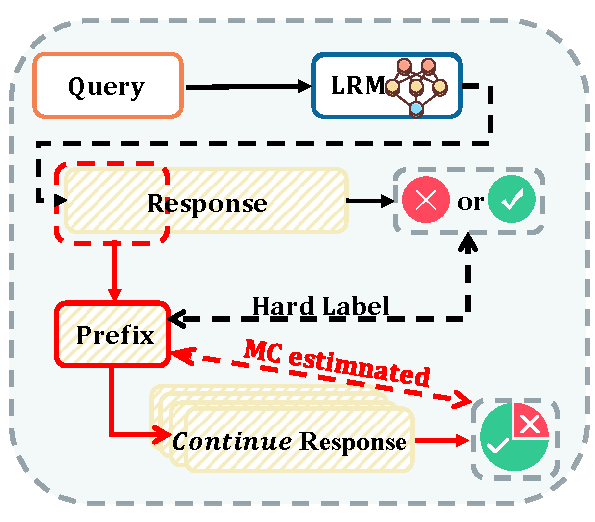
\includegraphics[width=0.44\columnwidth]{figures/Data_Construction.pdf}
%   \vspace{-0.8em}
%   \caption{MC-based construction of prefix–potential supervision.}
%   \label{fig:Data_Construction}
%   \vspace{-0.6em}
% \end{wrapfigure}
% Our data construction procedure, illustrated in Figure~\ref{fig:Data_Construction}, proceeds as follows:

% \paragraph{Prefix generation.} For each problem in the training set, we use the LRM to generate a prefix $p$ that forms part of a complete reasoning trajectory.

% \paragraph{Potential estimation via MC rollouts.} To estimate the potential of $p$, we fix the prefix and generate $K$ continuations under a high temperature. This procedure, known as \textbf{MC rollouts}, produces a set of full-length responses $\{\tau'_{1}, \tau'_{2}, \ldots, \tau'_{K}\}$.

% \paragraph{MC score calculation.} We evaluate each response for correctness (1 if correct and 0 otherwise). The \textbf{MC-estimated success probability} $s^{mc}$ for prefix $p$ is defined as the empirical accuracy of these samples:
% \begin{equation} \small
%     s^{mc} = \frac{1}{K} \sum_{j=1}^{K} \text{is\_correct}(\tau'_{j}).
% \end{equation}
% The resulting \textbf{MC-estimated label} $s^{mc} \in [0.0, 1.0]$ provides a fine-grained probabilistic target.


\section{Related Work}
\subsection{Parallel Reasoning}
\label{subsec:related_parallel}
Parallel reasoning, which generates multiple trajectories to verify or aggregate answers, has become a standard paradigm for enhancing LRM performance. 
A recent survey by ~\cite{wang2025parallel} systematically categorizes these approaches into three dimensions:
\textbf{(1) Non-interactive Reasoning}, which generates independent paths without communication, including majority voting in \textit{Self-Consistency}~\cite{wang2022self}, ranking in \textit{Best-of-N}~\cite{brown2024large}, and structured exploration in \textit{Tree-of-Thoughts}~\cite{yao2023tree}.
\textbf{(2) Interactive Reasoning}, which enables active information exchange among paths, for example, internal state sharing in \textit{Leap}~\cite{luo2025peers} or multi-agent collaboration~\cite{chan2023chamele}.
\textbf{(3) Efficiency Optimization}, which focuses on accelerating decoding mechanics, such as speculative decoding in \textit{Medusa}~\cite{cai2024medusa}.
Although these methods enhance reasoning performance, they still suffer from substantial inference costs, which remain a major limitation.

% Parallel reasoning, which generates multiple trajectories to verify or aggregate answers, has become a standard paradigm for enhancing LRM performance. 
% A recent survey by~\cite{wang2025parallel} systematically categorizes these approaches into three dimensions:
% \textbf{(1) Non-interactive Reasoning}, which generates independent paths without communication, including majority voting in \textit{Self-Consistency}~\cite{wang2022self}, ranking in \textit{Best-of-N}~\cite{brown2024large}, and structured exploration in \textit{Tree-of-Thoughts}~\cite{yao2023tree}.
% \textbf{(2) Interactive Reasoning}, which enables active information exchange among paths, for example, internal state sharing in \textit{Leap}~\cite{luo2025peers} or multi-agent collaboration~\cite{chan2023chamele}.
% \textbf{(3) Efficiency Optimization}, which focuses on accelerating decoding mechanics, such as speculative decoding in \textit{Medusa}~\cite{cai2024medusa}.
% However, while efficiency optimization reduces latency per token, it does not address the redundant computation of futile paths.
% Consequently, despite performance gains, parallel reasoning still suffers from prohibitive total inference costs.


\subsection{Path Pruning (Prefix Rejection)}
% To mitigate the high inference cost of parallel reasoning, path pruning strategies aim to terminate unpromising trajectories early. Consistent with the taxonomy in Section~\ref{sec:taxonomy}, we categorize existing works based on signal source and learnability. 
% % Regarding \textbf{external} signals, \textbf{non-learnable} methods like SlimSC~\cite{hong2025slimsc} prune paths utilizing heuristic metrics such as semantic similarity to minimize redundancy, while \textbf{learnable} approaches (Type~\ref{type:aux}) rely on trained verifiers—ranging from discriminative classifiers in DeepPrune~\cite{tu2025deepprune} to generative verifiers in ThinkPRM~\cite{khalifa2025process}. 
% Regarding \textbf{external} signals, \textbf{non-learnable} methods (Type~\ref{type:heuristic}) like SlimSC~\cite{hong2025slimsc} prune paths utilizing heuristic metrics such as semantic similarity to minimize redundancy, while \textbf{learnable} approaches (Type~\ref{type:aux}) rely on trained verifiers—ranging from discriminative classifiers in DeepPrune~\cite{tu2025deepprune} to generative verifiers in ThinkPRM~\cite{khalifa2025process}. 
% Shifting to \textbf{internal} sources, \textbf{non-learnable} methods (Type~\ref{type:stats}) derive signals directly from intrinsic statistics, such as the confidence-based DeepConf~\cite{fu2025deepthink} or entropy-based metrics~\cite{sharma2025thinkjust}.

% Notably, \textbf{prior works} leave the quadrant of \textbf{internal learnable} modules (Type~\ref{type:module}) unexplored. \textbf{\textbf{STOP}} is designed to bridge this gap, utilizing a trainable adapter to extract rich internal semantics, thus offering a solution that is both structurally efficient and data-driven.
To mitigate the high inference cost of parallel reasoning, path pruning strategies aim to terminate unpromising trajectories early. Consistent with the taxonomy in Section~\ref{sec:taxonomy}, we categorize existing works based on signal source and learnability.

Regarding \textbf{external} signals, \textbf{non-learnable} methods (Type~\ref{type:heuristic}) like SlimSC~\cite{hong2025slimsc} prune paths utilizing heuristic metrics such as semantic similarity to minimize redundancy.
In contrast, \textbf{learnable} approaches (Type~\ref{type:aux}) rely on trained verifiers. This category encompasses discriminative classifiers used in DeepPrune~\cite{tu2025deepprune} and LaBoR~\cite{liao2025lost}, as well as generative verifiers in ThinkPRM~\cite{khalifa2025process} and multi-agent frameworks like MAV~\cite{lifshitz2025multi}.
Shifting to \textbf{internal} sources, \textbf{non-learnable} methods (Type~\ref{type:stats}) derive signals directly from intrinsic statistics. Representative works include confidence-based estimation in DeepConf~\cite{fu2025deepthink} and AdaDec~\cite{he2025adadec}, or entropy-based metrics in Think Just Enough~\cite{sharma2025thinkjust}.

Notably, \textbf{prior works} leave the quadrant of \textbf{internal learnable} modules (Type~\ref{type:module}) unexplored. \textbf{\textbf{STOP}} is designed to bridge this gap, utilizing a trainable adapter to extract rich internal semantics, thus offering a solution that is both structurally efficient and data-driven.

\begin{figure}[t]
  \centering
  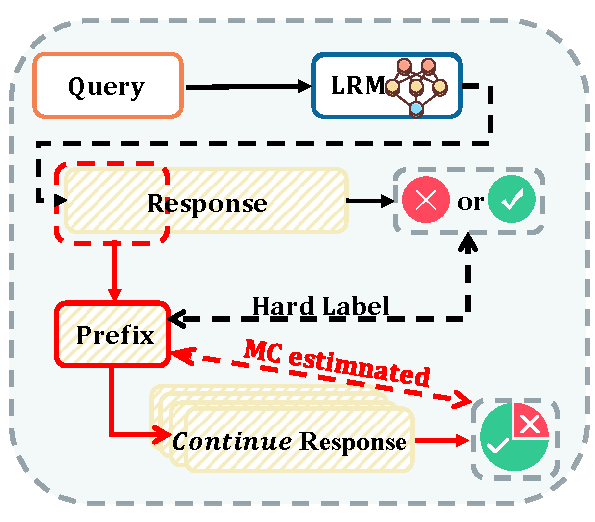
\includegraphics[width=0.8\columnwidth]{figures/Data_Construction.pdf}
  \caption{MC-based construction of prefix--potential supervision.}
  \label{fig:Data_Construction}
  \vspace{-2mm}
\end{figure}


\section{Data Construction Details}
\label{app:data_construction}

To train our \textbf{STOP} module, we require a dataset that directly maps prefixes of reasoning paths to the probability that the final answer succeeds. A single binary label on a complete path provides an insufficient and noisy signal, because a promising prefix may still end in an accidental failure, while a flawed prefix may occasionally be recovered by chance. Therefore, we construct a dataset of \texttt{(prefix, success probability)} pairs using \textbf{Monte Carlo (MC) estimation}~\cite{wang2024mathshepherd,zhao2025genprm}.

\subsection{Source Benchmarks and Decontamination}
We constructed a supervised fine-tuning dataset derived from high-quality mathematical and scientific benchmarks. Specifically, we aggregated approximately 1,000 problems from the \textbf{AIME} competition (spanning years 1984 to 2023)~\cite{maa2024aime,maa2025aime}, augmented with the non-Diamond portion of the \textbf{GPQA} dataset~\cite{rein2024gpqa}. 
\textit{Crucially, to ensure zero data leakage, we strictly excluded the evaluation sets from this training corpus: specifically, \textbf{AIME 2024}, \textbf{AIME 2025}, and the \textbf{GPQA Diamond} subset were entirely removed.}

\subsection{Model-Specific Construction Pipeline}
Since reasoning capabilities vary across model scales, we adopted a \textbf{model-specific pipeline} where each LRM (e.g., 1.5B) generates its own training data. The procedure proceeds as follows:

\paragraph{Difficulty Stratification (Filtering).}
Before generating prefixes, we first filter source problems to focus on the model's \textit{learnable boundary}. For each problem, we generate $N=32$ reasoning paths and calculate the pass rate. We explicitly exclude \textbf{trivial samples} ($>28$ correct answers) that the model has already mastered, as well as \textbf{intractable samples} ($<4$ correct answers) likely beyond its current capacity. This ensures that the training data consists of problems where the pruning signal is most valuable.

\begin{table}[t]
\centering
\small
\setlength{\tabcolsep}{4pt}
\caption{\textbf{Statistics of model-specific training data.} Prefixes are extracted from Math (AIME) and Science (GPQA). Data volume decreases for larger models due to filtering of trivial samples.}
\label{tab:training_data_stats}
\begin{tabular}{l c c c}
\toprule
\textbf{Model} & \textbf{Math} & \textbf{Science} & \textbf{Total} \\
\midrule
DS-Qwen-2.5-1.5B & 14,816 & 8,448 & \textbf{23,264} \\
DS-Qwen-2.5-7B   & 12,092 & 5,666 & \textbf{17,758} \\
DS-Qwen-3-8B     & 10,848 & 4,456 & \textbf{15,304} \\
GPT-OSS-20B      & 7,872  & 2,378 & \textbf{10,250} \\
\bottomrule
\end{tabular}
\vspace{-3mm}
\end{table}

\paragraph{Prefix Generation.} 
From the retained problems, we use the LRM to generate a prefix $p$ that forms part of a complete reasoning trajectory. To simulate a realistic mid-generation checkpoint, we truncate these paths at a fixed length of \textbf{$L_{\text{prefix}} = 2{,}048$} tokens.

\paragraph{Potential Estimation via MC Rollouts.}
% \begin{wrapfigure}{r}{0.85\columnwidth}
%   \centering
%   \vspace{-0.6em}
%   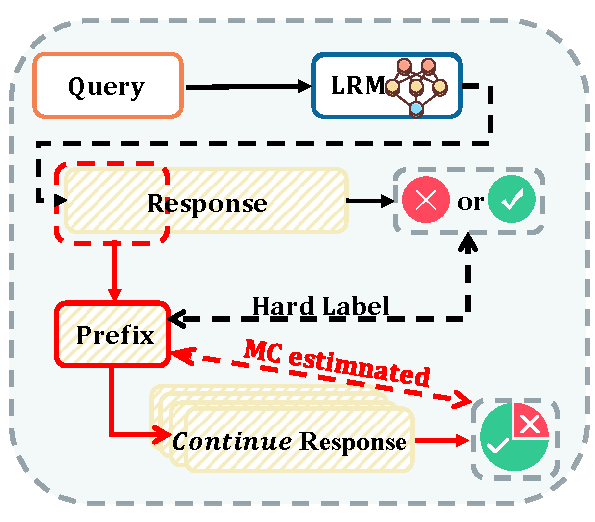
\includegraphics[width=0.44\columnwidth]{figures/Data_Construction.pdf}
%   \vspace{-0.8em}
%   \caption{MC-based construction of prefix–potential supervision.}
%   \label{fig:Data_Construction}
%   \vspace{-0.6em}
% \end{wrapfigure}
To estimate the potential of $p$, we fix the prefix and generate \textbf{$K=32$} continuations under a temperature of $0.6$. This procedure produces a set of full-length responses $\{\tau'_{1}, \tau'_{2}, \ldots, \tau'_{K}\}$.


\paragraph{MC Score Calculation.}
We evaluate each response for correctness (1 if correct and 0 otherwise). The MC-estimated success probability $s^{mc}$ is defined as the empirical accuracy:
\begin{equation} \small
    s^{mc} = \frac{1}{K} \sum_{j=1}^{K} \text{is\_correct}(\tau'_{j}).
\end{equation}
The resulting label $s^{mc} \in [0.0, 1.0]$ provides a fine-grained probabilistic target used to train the STOP module.


\paragraph{Data Statistics and Insights.}
Table~\ref{tab:training_data_stats} summarizes the composition of the constructed datasets. 
We observe a distinct \textbf{inverse scaling trend}: as the model size increases, the number of valid training samples decreases (e.g., from 23,264 for 1.5B to 10,250 for 20B). 
This confirms the efficacy of our difficulty stratification strategy: larger models (e.g., GPT-OSS-20B) achieve high pass rates ($>28/32$) on a larger portion of the source benchmarks, causing these ``trivial'' instances to be filtered out. Consequently, the training data naturally adapts to focus on the \textit{learnable boundary} specific to each model's capability.

% \begin{table}[h]
% \centering
% \small
% \caption{\textbf{Statistics of Model-Specific Training Data.} The dataset is composed of prefixes extracted from Math (AIME) and Science (GPQA) domains. The volume of data decreases for larger models as they master more source problems, triggering the ``trivial sample'' exclusion filter.}
% \label{tab:training_data_stats}
% \begin{tabular}{l c c c}
% \toprule
% \textbf{Model} & \textbf{Math Pairs (AIME)} & \textbf{Science Pairs (GPQA)} & \textbf{Total Training Pairs} \\
% \midrule
% DS-Qwen-2.5-1.5B & 14,816 & 8,448 & \textbf{23,264} \\
% DS-Qwen-2.5-7B   & 12,092 & 5,666 & \textbf{17,758} \\
% DS-Qwen-3-8B     & 10,848 & 4,456 & \textbf{15,304} \\
% GPT-OSS-20B      & 7,872  & 2,378 & \textbf{10,250} \\
% \bottomrule
% \end{tabular}
% \end{table}



\subsection{Training Cost Details}
\label{app:training_cost}

Constructing the MC supervision dataset requires sampling multiple continuations per prefix (e.g., $K=32$) as described in Section~\ref{subsec:motivation}.
In practice, we find that moderate sampling budgets provide a good balance between estimation stability and computational cost, as also reflected in our ablation results.
We report the estimated cost across different model scales in Table~\ref{tab:training_cost}.

These costs correspond to a one-time data construction process.
Once constructed, the dataset can be reused across training runs and model variants, amortizing the cost of data construction.
The trained STOP module introduces negligible overhead during inference.
These costs are reported to provide transparency and should be interpreted as approximate estimates depending on implementation and hardware configurations.
% \begin{table}[h]
% \centering
% \small
% \caption{\textbf{Training Cost for MC Supervision Construction.} 
% We report the number of training pairs and the estimated wall-clock cost (in 8$\times$H100 GPU hours) required to construct the dataset with $K=32$ Monte Carlo samples per prefix.}
% \label{tab:training_cost}
% \begin{tabular}{lcccc}
% \toprule
% \textbf{Model} & \textbf{Math} & \textbf{Science} & \textbf{Total Training Pairs} & \textbf{8$\times$H100 Hours} \\
% \midrule
% DS-Qwen-2.5-1.5B & 14,816 & 8,448 & \textbf{23,264} & 43.08 \\
% DS-Qwen-2.5-7B   & 12,092 & 5,666 & \textbf{17,758} & 39.46 \\
% DS-Qwen-3-8B     & 10,844 & 4,456 & \textbf{15,304} & 37.79 \\
% GPT-OSS-20B      & 7,872  & 2,378 & \textbf{10,250} & 75.93 \\
% \bottomrule
% \end{tabular}
% \end{table}
\begin{table*}[t]
\centering
\small
\caption{\textbf{Training Cost for MC Supervision Construction.} 
We report the number of training pairs and the estimated wall-clock cost (in 8$\times$H100 GPU hours) required to construct the dataset with $K=32$ Monte Carlo samples per prefix.}
\label{tab:training_cost}
\begin{tabular}{lcccc}
\toprule
\textbf{Model} & \textbf{Math} & \textbf{Science} & \textbf{Total Training Pairs} & \textbf{8$\times$H100 Hours} \\
\midrule
DS-Qwen-2.5-1.5B & 14,816 & 8,448 & \textbf{23,264} & 43.08 \\
DS-Qwen-2.5-7B   & 12,092 & 5,666 & \textbf{17,758} & 39.46 \\
DS-Qwen-3-8B     & 10,844 & 4,456 & \textbf{15,304} & 37.79 \\
GPT-OSS-20B      & 7,872  & 2,378 & \textbf{10,250} & 75.93 \\
\bottomrule
\end{tabular}
\vspace{-3mm}
\end{table*}



\begin{table*}[t]
\centering
\small
\caption{\textbf{Training hyperparameters across model scales.}}
\label{tab:training_hyperparams}
\begin{tabular}{lcccc}
\toprule
\textbf{Hyperparameter} & \textbf{1.5B} & \textbf{7B} & \textbf{8B} & \textbf{20B} \\
\midrule
Per-Device Batch Size & 16 & 8 & 8 & 2 \\
Gradient Accumulation & 1 & 2 & 2 & 8 \\
Learning Rate & $2 \times 10^{-5}$ & $2 \times 10^{-5}$ & $2 \times 10^{-5}$ & $2 \times 10^{-5}$ \\
LoRA Rank ($r$) & 128 & 256 & 256 & 2048 \\
LoRA Alpha ($\alpha$) & 256 & 512 & 512 & 4096 \\
Target Modules & All Linear & All Linear & All Linear & All Linear \\
Optimizer & AdamW & AdamW & AdamW & AdamW \\
Max Prefix Length & 2048 & 2048 & 2048 & 2048 \\
Training Epochs & 15 & 15 & 15 & 15 \\
Precision & \texttt{bf16} & \texttt{bf16} & \texttt{bf16} & \texttt{bf16} \\
\bottomrule
\end{tabular}
\vspace{-3mm}
\end{table*}


% \begin{figure}[t]
%   \centering
%   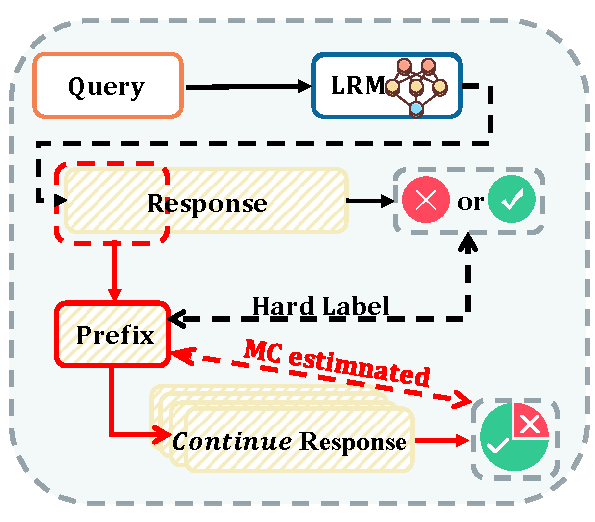
\includegraphics[width=\columnwidth]{figures/Data_Construction.pdf}
% \caption{MC-based construction of prefix–potential supervision.}
%   \label{fig:optimal_pruning_ratio_with_fit}
% \end{figure}



% \section{Detailed Experimental Settings}
% \label{app:exp_setup}

% \subsection{Infrastructure and Sampling Configuration}
% \label{app:infrastructure}
% \textbf{Infrastructure.}
% All experiments were conducted on NVIDIA H100 (80GB) GPUs.
% We utilized the \texttt{vLLM} framework~\cite{kwon2023efficient} to support efficient batched inference during the evaluation phases.

% \noindent \textbf{Sampling Configuration.}
% To ensure consistency across all pruning methods, we adopted a unified generation configuration.
% Specifically, the temperature was set to $0.6$, top-$p$ to $0.95$, and top-$k$ to $40$.
% The maximum generation length was set to $16{,}384$ tokens for the 1.5B and 7B models, and $32{,}768$ tokens for the 8B and 20B models.
% For \texttt{gpt-oss} models, the reasoning effort was set to ``medium''.

% \subsection{Source Datasets and Evaluation Protocol}
% \label{app:datasets}

% \noindent\textbf{Source Benchmarks.}
% To enhance the general reasoning capability of the base models, we constructed a supervised fine-tuning dataset derived from high-quality mathematical and scientific benchmarks.
% Specifically, we aggregated approximately 1,000 problems from the \textbf{AIME} competition (spanning years 1984 to 2023)~\cite{maa2024aime,maa2025aime}, augmented with the non-Diamond portion of the \textbf{GPQA} dataset~\cite{rein2024gpqa}.

% \noindent\textbf{Evaluation Protocol.}
% We strictly adhered to established evaluation protocols to ensure fair comparison and reproducibility. The \textbf{GPQA-Diamond} subset, consisting of 198 high-difficulty questions, was reserved exclusively as a held-out test set. Consequently, all remaining GPQA questions were used solely during the training stage. This rigorous separation guarantees zero information leakage from the training corpus to the evaluation benchmarks.

% \noindent\textbf{Soft Label Generation.}
% Following the Monte Carlo estimation pipeline described in Section ~\ref{sec:Data_Construction}, we constructed the training targets with the following specific parameters: we sampled \textbf{$K=32$} continuations for each prefix using a temperature of \textbf{$0.6$} and top-$p$ of \textbf{$0.95$}. The success probability $L_{MC}$ was derived from the pass rate of these completions.


% \subsection{STOP Module Training Details}
% \label{app:stop_training}
% We implemented \textbf{STOP} ($S_{\text{module}}$) using the HuggingFace Transformers library integrated with the PEFT library. The parameters of the base LRM remained frozen throughout the training process.

% \noindent \textbf{Model Configuration.}
% \textbf{STOP} is implemented as a LoRA adapter. We targeted all linear modules in the base model, specifically: \texttt{q\_proj}, \texttt{k\_proj}, \texttt{v\_proj}, \texttt{o\_proj}, \texttt{gate\_proj}, \texttt{up\_proj}, and \texttt{down\_proj}. The LoRA configuration used a rank of $r=128$, a scaling factor of $\alpha=256$, and a dropout rate of $0.05$.

% \noindent \textbf{Training Hyperparameters.}
% We trained the module using the AdamW optimizer with a learning rate of $1\times10^{-4}$ and a cosine learning rate scheduler (warmup ratio set to $0.03$).
% The effective batch size was set to $16$ (achieved via a per-device batch size of $4$ with $4$ gradient accumulation steps).
% Training was performed for $3$ epochs on the constructed dataset, with a maximum sequence length of $4{,}096$ tokens.

% \subsection{Baseline Descriptions}
% \label{app:baselines}
% We provide additional details on the baseline implementations used in Section~\ref{sec:Comprehensive}:
% \begin{itemize}
%     \item \textbf{SlimSC ($S_{\text{heuristic}}$):} Computes the pairwise Jaccard similarity between the current generation and previously explored reasoning paths. It prunes trajectories that exhibit high semantic redundancy to ensure diversity.
%     \item \textbf{External PRM ($S_{\text{aux}}$):} Relies on a separate, trained Process Reward Model (PRM) to score generated prefixes. We used the official checkpoints released by the authors where available.
%     \item \textbf{DeepConf ($S_{\text{stats}}$):} Estimates confidence by computing perplexity and entropy directly from the model logits of the generated tokens, serving as a non-learnable internal baseline.
% \end{itemize}



% \section{Prompt Templates and Input Format}
% \label{app:prompts}

% To ensure rigorous reproducibility, we detail the exact prompt templates and input construction used in our experiments. We utilized the standard zero-shot Chain-of-Thought (CoT) format.

% \begin{tcolorbox}[
%     colback=white, 
%     colframe=gray!60!black, 
%     title=\textbf{Prompt Templates \& Input Format},
%     fonttitle=\bfseries\large,
%     boxrule=1pt,
%     arc=2mm
% ]
% % --- GPQA ---
% \noindent\textbf{\textcolor{blue}{GPQA:}}

% \noindent\texttt{Please show your choice in the answer field with only the choice letter, e.g., "ANSWER": "C".}

% \vspace{1em} % 增加一点间距

% % --- Math ---
% \noindent\textbf{\textcolor{blue}{Math Tasks (AIME, HMMT, BRUMO):}}

% \noindent\texttt{Please reason step by step, and put your final answer within \textbackslash boxed\{\}.}

% \vspace{1em}
% \tcbline % 分割线
% \vspace{0.5em}

% % --- STOP Format ---
% \noindent\textbf{STOP Module Input Sequence:}

% The input to the \textbf{STOP} module is formed by concatenating the user query (with the above instruction), the generated reasoning prefix, and the special token:

% \begin{center}
% \texttt{[User Prompt] [Generated Reasoning Prefix] [STOP]}
% \end{center}

% \end{tcolorbox}

% \section{Training Details of STOP}
% \label{app:hyper_STOP}

% We developed a custom training pipeline utilizing the Hugging Face \texttt{Accelerate} and \texttt{PEFT} libraries. All experiments were conducted on 8 NVIDIA H100 GPUs using a LoRA-only approach, where we froze the base model parameters and strictly trained low-rank adapters attached to all linear layers. The specific hyperparameters, including the varying LoRA configurations for different model scales, are detailed in Table~\ref{tab:sft_hyperparameters}.

% \begin{table}[H]
% \centering
% \caption{Hyperparameters for \textbf{STOP} module training. The per-device batch size was set to 16 with 4 gradient accumulation steps, resulting in a global effective batch size of 512.}
% \label{tab:sft_hyperparameters}
% % \resizebox{\textwidth}{!}{% 自适应调整宽度
% \begin{tabular}{lcccc}
% \toprule
% \textbf{Hyperparameter} & \textbf{1.5B} & \textbf{7B} & \textbf{8B} & \textbf{20B} \\
% \midrule
% Per-Device Batch Size & 16 & 8 & 8 & 2 \\
% Gradient Accumulation & 1 & 2 & 2 & 8 \\
% Learning Rate & $2 \times 10^{-5}$ & $2 \times 10^{-5}$ & $2 \times 10^{-5}$ & $2 \times 10^{-5}$ \\
% LoRA Rank ($r$) & 128 & 256 & 256 & 2048 \\
% LoRA Alpha ($\alpha$) & 256 & 512 & 512 & 4096 \\
% Target Modules & All Linear & All Linear & All Linear & All Linear \\
% Optimizer & AdamW & AdamW & AdamW & AdamW \\
% Max Prefix Length & 2048 & 2048 & 2048 & 2048 \\
% Training Epochs & 15 & 15 & 15 & 15 \\
% Precision & \texttt{bf16} & \texttt{bf16} & \texttt{bf16} & \texttt{bf16} \\
% \bottomrule
% \end{tabular}
% % }
% \end{table}




\section{Detailed Experimental Settings}
\label{app:exp_setup}

In this appendix, we provide the complete experimental details to ensure reproducibility, covering infrastructure, datasets, input formats, training hyperparameters, and baseline implementations.

\subsection{Infrastructure and Sampling Configuration}
\label{app:infrastructure}
\noindent\textbf{Infrastructure.}
All experiments were conducted on NVIDIA H100 (80GB) GPUs.
We utilized the \texttt{vLLM} framework~\cite{kwon2023efficient} to support efficient batched inference during the evaluation phases.

\noindent \textbf{Sampling Configuration.}
To ensure consistency across all pruning methods, we adopted a unified generation configuration.
Specifically, the temperature was set to $0.6$, top-$p$ to $0.95$, and top-$k$ to $40$.
The maximum generation length was set to $16{,}384$ tokens for the 1.5B and 7B models, and $32{,}768$ tokens for the 8B and 20B models.
For \texttt{gpt-oss} models, the reasoning effort was set to ``medium''.

\subsection{Evaluation Protocol}
\label{app:datasets}

% \noindent\textbf{Source Benchmarks.}
% To enhance the general reasoning capability of the base models, we constructed a supervised fine-tuning dataset derived from high-quality mathematical and scientific benchmarks.
% Specifically, we aggregated approximately 1,000 problems from the \textbf{AIME} competition (spanning years 1984 to 2023)~\cite{maa2024aime,maa2025aime}, augmented with the non-Diamond portion of the \textbf{GPQA} dataset~\cite{rein2024gpqa}.

We strictly adhered to established evaluation protocols to ensure fair comparison and reproducibility. The \textbf{GPQA-Diamond} subset, consisting of 198 high-difficulty questions, was reserved exclusively as a held-out test set. Consequently, all remaining GPQA questions were used solely during the training stage. This rigorous separation guarantees zero information leakage from the training corpus to the evaluation benchmarks.


\subsection{Prompt Templates and Input Format}
\label{app:prompts}

To ensure rigorous reproducibility, we detail the exact prompt templates and input construction used in our experiments. We utilized the standard zero-shot Chain-of-Thought (CoT) format.

\begin{tcolorbox}[
    colback=white, 
    colframe=gray!60!black, 
    title=\textbf{Prompt Templates \& Input Format},
    fonttitle=\bfseries\large,
    boxrule=1pt,
    arc=2mm
]
% --- GPQA ---
\noindent\textbf{\textcolor{blue}{GPQA:}}

\noindent\texttt{Please show your choice in the answer field with only the choice letter, e.g., "ANSWER": "C".}

\vspace{1em} 

% --- Math ---
\noindent\textbf{\textcolor{blue}{Math Tasks (AIME, HMMT, BRUMO):}}

\noindent\texttt{Please reason step by step, and put your final answer within \textbackslash boxed\{\}.}

\vspace{1em}
\tcbline 
\vspace{0.5em}

% --- STOP Format ---
% \noindent\textbf{STOP Module Input Sequence:}

% The input to the \textbf{STOP} module is formed by concatenating the user query (with the above instruction), the generated reasoning prefix, and the special token:

% \begin{center}
% \texttt{[User Prompt] [Generated Reasoning Prefix] [STOP]}
% \end{center}
% --- STOP Format ---
\noindent\textbf{STOP Module Input Mechanism:}

To achieve zero-overhead verification, we do not re-encode the full text. Instead, the \textbf{STOP} token is appended directly to the \textbf{pre-computed KV cache} of the generated prefix.
Conceptually, this provides the module with the following effective context, allowing it to attend to the full history:

% \begin{center}
% \ttfamily
% \colorbox{gray!10}{[User Prompt] [Generated Reasoning Prefix] [STOP]}
% \end{center}
\begin{center}
\fcolorbox{gray!60}{gray!10}{
\parbox{0.9\columnwidth}{
\centering\ttfamily
[User Prompt] [Generated Reasoning Prefix] [STOP]
}}
\end{center}

\end{tcolorbox}

\subsection{STOP Module Training Details}
\label{app:training_details}

We developed a custom training pipeline utilizing the Hugging Face \texttt{Accelerate} and \texttt{PEFT} libraries. All experiments were conducted on 8 NVIDIA H100 GPUs using a LoRA-only approach. We froze the base model parameters and strictly trained low-rank adapters attached to \textbf{all linear layers} within the transformer blocks. 
Specifically, we targeted the full set of projections: \texttt{q\_proj}, \texttt{k\_proj}, \texttt{v\_proj}, \texttt{o\_proj}, \texttt{gate\_proj}, \texttt{up\_proj}, and \texttt{down\_proj}. 
The specific hyperparameters, including the varying LoRA configurations for different model scales, are detailed in Table~\ref{tab:training_hyperparams}.

% \begin{table}[H]
% \centering
% \caption{Hyperparameters for \textbf{STOP} module training. The per-device batch size was set to 16 with 4 gradient accumulation steps, resulting in a global effective batch size of 512.}
% \label{tab:sft_hyperparameters}
% % \resizebox{\textwidth}{!}{% Optional: un-comment if table is too wide
% \begin{tabular}{lcccc}
% \toprule
% \textbf{Hyperparameter} & \textbf{1.5B} & \textbf{7B} & \textbf{8B} & \textbf{20B} \\
% \midrule
% Per-Device Batch Size & 16 & 8 & 8 & 2 \\
% Gradient Accumulation & 1 & 2 & 2 & 8 \\
% Learning Rate & $2 \times 10^{-5}$ & $2 \times 10^{-5}$ & $2 \times 10^{-5}$ & $2 \times 10^{-5}$ \\
% LoRA Rank ($r$) & 128 & 256 & 256 & 2048 \\
% LoRA Alpha ($\alpha$) & 256 & 512 & 512 & 4096 \\
% Target Modules & All Linear & All Linear & All Linear & All Linear \\
% Optimizer & AdamW & AdamW & AdamW & AdamW \\
% Max Prefix Length & 2048 & 2048 & 2048 & 2048 \\
% Training Epochs & 15 & 15 & 15 & 15 \\
% Precision & \texttt{bf16} & \texttt{bf16} & \texttt{bf16} & \texttt{bf16} \\
% \bottomrule
% \end{tabular}
% % }
% \end{table}


\subsection{Baseline Descriptions}
\label{app:baselines}
We provide additional details on the baseline implementations used in Section~\ref{sec:Comprehensive}:
\begin{itemize}
    \item \textbf{SlimSC~\cite{hong2025slimsc} (Type~\ref{type:heuristic}):} Computes the pairwise Jaccard similarity between the current generation and previously explored reasoning paths. It prunes trajectories that exhibit high semantic redundancy to ensure diversity.
    \item \textbf{LaBoR~\cite{liao2025lost} (Type~\ref{type:aux}):} Relies on a separate, trained Process Reward Model (PRM) to score generated prefixes. We used the official checkpoints released by the authors where available.
    \item \textbf{DeepConf~\cite{fu2025deepthink} (Type~\ref{type:stats}):} Estimates confidence by computing perplexity and entropy directly from the model logits of the generated tokens, serving as a non-learnable internal baseline.
\end{itemize}


% \begin{table*}[t]
% \vspace{-14mm}
% \centering
% \caption{A Unified Taxonomy of Path Pruning Methods. We categorize methods based on the pruning signal source and learnability. \textbf{Type~\ref{type:module}} satisfies both \textbf{Desideratum~\ref{desideratum:internal}} (Internal) and \textbf{Desideratum~\ref{desideratum:learnable}} (Learnable).}
% \label{tab:taxonomy}
% \renewcommand{\arraystretch}{1.5} % Increase row height for readability
% \resizebox{0.95\linewidth}{!}{
% \begin{tabular}{l|c|c}
% \toprule
%  & \textbf{Non-Learnable} & \textbf{Learnable} \\
%  &  & (Desideratum~\ref{desideratum:learnable}) \\ \midrule

% \textbf{External Source} & \textbf{Type~\ref{type:heuristic}} & \textbf{Type~\ref{type:aux}} \\
%  & \begin{tabular}[c]{@{}c@{}}
% \textbf{SlimSC}~\cite{hong2025slimsc}
% \end{tabular} & \begin{tabular}[c]{@{}c@{}}
% \textbf{DeepPrune}~\cite{tu2025deepprune}, \textbf{LaBoR}~\cite{liao2025lost} \\
% \textbf{ThinkPRM}~\cite{khalifa2025process}, \textbf{MAV}~\cite{lifshitz2025multi}
% \end{tabular} \\ \midrule

% \textbf{Internal Source} & \textbf{Type~\ref{type:stats}} & \textbf{Type~\ref{type:module}} \\
% (Desideratum~\ref{desideratum:internal}) & \begin{tabular}[c]{@{}c@{}}
% \textbf{DeepConf}~\cite{fu2025deepthink}, 
% \textbf{AdaDec}~\cite{he2025adadec} \\
% \textbf{Think Just Enough}~\cite{sharma2025thinkjust}
% \end{tabular} & \begin{tabular}[c]{@{}c@{}}
% \textbf{STOP (Ours)}
% \end{tabular} \\ \bottomrule
% \end{tabular}
% }
% \end{table*}






% \section{Ablation: Data Quality vs. Architecture}
% \label{app:labor_t}

% \subsection{Motivation and Setup}
% A potential confounding factor in our main results is the quality of the training data. Since \textbf{STOP} is trained on a high-quality dataset constructed via Monte Carlo rollouts, it is natural to hypothesize that the observed performance gains mainly arise from superior supervision rather than from the $S_\text{module}$ architecture itself. To disentangle these two factors, we introduce a controlled baseline, \textbf{$S_\text{aux}^{\text{retrain}}$ (Retrained Early Pruning)}. Liao et al.~\cite{liao2025lost} propose an Early Pruning strategy based on an external Process Reward Model (PRM), specifically \texttt{Qwen2.5-Math-PRM-7B}, but their model is not trained on our MC-estimated soft labels. For a fair comparison, we adopt the same architecture and fine-tune it on the \emph{same dataset} of prefix--success probability pairs used to train \textbf{STOP}. This comparison isolates the architectural effect between an internal, learnable module ($S_\text{module}$) with access to full hidden states and an external reward model ($S_\text{aux}$) that relies only on token-level outputs, thereby ruling out data quality as the sole source of improvement. \textbf{Note:} Because the backbone of $S_\text{aux}$ is specialized for mathematics, we exclude the GPQA (Science) benchmark from this ablation, as the external PRM lacks sufficient domain knowledge for scientific reasoning.

% \subsection{Detailed Analysis}
% Table~\ref{tab:main_results_LaBor} reports results across models and benchmarks. We observe that $S_\text{aux}^{\text{retrain}}$ consistently outperforms the standard $S_\text{aux}$ baseline, which is typically trained on public PRM datasets or heuristic labels. This result confirms that MC-estimated soft labels provide a stronger and more informative supervision signal than conventional binary labels, even for external reward models. More importantly, despite being trained on identical data, \textbf{\textbf{STOP} consistently outperforms $S_\text{aux}^{\text{retrain}}$} across different model scales. For example, at the 1.5B scale, \textbf{STOP} achieves higher avg@8 on AIME 25 (26.67\% vs.\ 24.16\%) and BRUMO 25 (33.75\% vs.\ 32.50\%), while at the 7B scale it surpasses $S_\text{aux}^{\text{retrain}}$ on AIME 24 (61.67\% vs.\ 59.17\%). In addition, while $S_\text{aux}$ is restricted to mathematical tasks due to its specialized backbone, \textbf{STOP}, implemented via LoRA, naturally generalizes to the scientific domain on GPQA during training, demonstrating greater flexibility. The only exception is a minor difference on DS-Qwen-3-8B for AIME 25 (72.92\% vs.\ 73.33\%), which lies within normal variance; in all other settings, \textbf{STOP} shows clear and consistent advantages.

% \subsection{Discussion: The Advantage of Internal Signals}
% The superiority of \textbf{STOP} ($S_\text{module}$) can be attributed to its ability to mitigate the \emph{information bottleneck} inherent in external evaluation. An external PRM ($S_\text{aux}$) judges reasoning quality solely from generated text, which is a discrete and low-dimensional projection of the model’s internal reasoning process and often discards subtle signals of uncertainty and coherence. In contrast, \textbf{STOP} is integrated directly into the generator and has access to dense internal representations, including hidden states and attention patterns. These internal signals preserve rich information about confidence and logical consistency that is largely lost during decoding. By leveraging such first-person internal signals, \textbf{STOP} evaluates the potential of a prefix more accurately than a third-person external reward model.


% \begin{table*}[t]
% \centering
% \caption{
% \textbf{Ablation Study: Architecture vs. Data.} Comparison of avg@8 and token efficiency. 
% $S_{\text{aux}}$ refers to the standard external PRM baseline (Early Pruning). 
% $S_{\text{aux}}^{\text{retrain}}$ denotes the same external architecture retrained on our MC-estimated data. 
% \textbf{STOP} ($S_{\text{module}}$) outperforms both, demonstrating that architectural access to internal states yields gains beyond data quality alone.
% Note: $S_{\text{aux}}$ variants are not evaluated on GPQA due to the domain limitation of the math-specialized PRM backbone.
% }
% \label{tab:main_results_LaBor}
% \resizebox{\textwidth}{!}{%
% \begin{tabular}{llcc cc cc cc}
% \toprule
% \multirow{2}{*}{\textbf{Model}} & \multirow{2}{*}{\textbf{Dataset}} 
% & \multicolumn{2}{c}{\textbf{Full Paths (Baseline)}} 
% & \multicolumn{2}{c}{\textbf{$S_\text{aux}$}} 
% & \multicolumn{2}{c}{\textbf{$S_\text{aux}^{\text{retrain}}$}} 
% & \multicolumn{2}{c}{\textbf{$S_\text{module}$}} \\
% \cmidrule(lr){3-4} \cmidrule(lr){5-6} \cmidrule(lr){7-8} \cmidrule(lr){9-10}
% & &avg@8|64 ($\uparrow$) & Tokens ($\downarrow$) & avg@8|64 ($\uparrow$) & Tokens (\% $\downarrow$) & avg@8|64 ($\uparrow$) & Tokens (\% $\downarrow$) & avg@8|64 ($\uparrow$) & Tokens (\% $\downarrow$) \\
% \midrule
% \midrule
% \multirow{5}{*}{DS-Qwen-2.5-1.5B} 
% & AIME24 & 30.10 & 782.3k & 32.50 & 325.9k~(-58.34\%) &\underline{37.50} & \underline{318.2k}~(-59.33\%) & \textbf{37.92} & \textbf{204.3k}~(-73.88\%)\\
% & AIME25 & 22.76 & 784.8k & \underline{24.17} & 325.0k~(-58.59\%) & 24.16 & \underline{323.2k}~(-58.82\%) & \textbf{26.67} & \textbf{206.6k}~(-73.68\%)\\
% & BRUMO25 & 30.99 & 774.6k & \underline{31.67} & 325.6k~(-57.96\%) & \underline{32.50} & \underline{320.5k}~(-58.62\%) & \textbf{33.75} & \textbf{204.4k}~(-73.61\%) \\
% & HMMT25 & 15.05 & 856.4k & 15.00 & 337.2k~(-60.63\%) &\underline{16.67} & \underline{333.8k}~(-61.03\%) & \textbf{17.92} & \textbf{215.5k}~(-74.84\%)\\
% & GPQA-D & 33.08 & 550.9k & - & - & - & - & \textbf{48.42} & \textbf{179.4k}~(-67.43\%) \\
% \midrule
% \multirow{5}{*}{DS-Qwen-2.5-7B} 
% & AIME24 & 54.69 & 666.2k & 54.58 & 312.5k~(-53.09\%) & \underline{59.17} & \underline{308.6k}~(-53.68\%) & \textbf{61.67} & \textbf{189.0k}~(-71.63\%) \\
% & AIME25 & 39.67 & 703.0k & 39.17 & 317.6k~(-54.82\%) & \underline{37.08} & \underline{315.5k}~(-55.13\%) & \textbf{42.50} & \textbf{197.5k}~(-71.91\%) \\
% & BRUMO25 & 50.99 & 656.6k & 51.25 & 312.1k~(-52.46\%) & \underline{53.33} & \underline{309.1k}~(-52.92\%) & \textbf{56.67} & \textbf{190.2k}~(-71.03\%)\\
% & HMMT25 & 23.91 & 808.9k & 23.33 & 330.8k~(-59.11\%) & \underline{24.17} & \underline{328.8k}~(-59.35\%) & \textbf{27.08} & \textbf{211.6k}~(-73.84\%)\\
% & GPQA-D & 45.95 & 443.8k & - & - & - & - & \textbf{55.75} & \textbf{165.9k}~(-62.61\%)\\
% \midrule
% \multirow{5}{*}{DS-Qwen-3-8B} 
% & AIME24 & 76.93 & 1361k & \underline{78.75} & 398.4k~(-70.73\%) & 77.92 & \underline{396.5k}~(-70.87\%) & \textbf{79.17} & \textbf{279.0k}~(-79.51\%)\\
% & AIME25 & 70.68 & 1427k & \underline{72.50} & 408.4k~(-71.39\%) & \textbf{73.33} & \underline{407.5k}~(-71.44\%) & \underline{72.92} & \textbf{290.9k}~(-79.62\%)\\
% & BRUMO25 & 75.00 & 1320k & \underline{75.83} & 394.9k~(-70.10\%) & 75.00 & \underline{396.1k}~(-70.01\%) & \textbf{78.75} & \textbf{277.5k}~(-78.98\%)\\
% & HMMT25 & 51.04 & 1601k & 50.83 & 427.8k~(-73.28\%) & \underline{52.08} & \underline{427.7k}~(-73.28\%) & \textbf{54.58} & \textbf{311.7k}~(-80.53\%)\\
% & GPQA-D & 56.87 & 652.6k & - & - & - & - & \textbf{63.32} & \textbf{193.5k}~(-70.35\%)\\
% \midrule
% \multirow{5}{*}{GPT-OSS-20B}
% & AIME24 & 75.26 & 594.2k & \underline{76.25} & 299.8k~(-49.55\%) & 74.16 & \underline{302.5k}~(-49.09\%) & \textbf{77.50} & \textbf{184.4k}~(-68.98\%) \\
% & AIME25 & \underline{70.99} & 673.4k & 69.17 & 311.7k~(-53.71\%) & 69.58 & \underline{310.4k}~(-53.91\%) & \textbf{75.42} & \textbf{191.1k}~(-71.62\%)\\
% & BRUMO25 & \underline{68.02} & 575.6k & 66.25 & 298.8k~(-48.09\%) & 67.50 & \underline{297.9k}~(-48.24\%) & \textbf{70.00} & \textbf{183.6k}~(-68.11\%) \\
% & HMMT25 & \underline{48.13} & 910.8k & 45.42 & 336.9k~(-63.01\%) & 48.75 & \underline{333.3k}~(-63.41\%) & \textbf{52.92} & \textbf{216.1k}~(-76.27\%)\\
% & GPQA-D & 65.55 & 277.2k & - & - & - & - & \textbf{77.46} & \underline{143.4k}~(-48.26\%)\\
% \bottomrule
% \end{tabular}
% }
% \end{table*}

\section{Ablation: Data Quality vs. Architecture}
\label{app:labor_t}

\subsection{Motivation and Setup}
A potential confounding factor in our main results is the quality of the training data. Since \textbf{STOP} is trained on a high-quality dataset constructed via Monte Carlo rollouts, it is natural to hypothesize that the observed performance gains mainly arise from superior supervision rather than from the \textbf{Type~\ref{type:module}} architecture itself. To disentangle these two factors, we introduce a controlled baseline, \textbf{Type~\ref{type:aux}${}^{\text{retrain}}$ (Retrained Early Pruning)}. LaBoR~\cite{liao2025lost} propose an Early Pruning strategy based on an external Process Reward Model (PRM), specifically \texttt{Qwen2.5-Math-PRM-7B}, but their model is not trained on our MC-estimated soft labels. For a fair comparison, we adopt the same architecture and fine-tune it on the \emph{same dataset} of prefix--success probability pairs used to train \textbf{STOP}. This comparison isolates the architectural effect between an internal, learnable method (\textbf{Type~\ref{type:module}}) with access to full hidden states and an external reward model (\textbf{Type~\ref{type:aux}}) that relies only on token-level outputs, thereby ruling out data quality as the sole source of improvement. \textbf{Note:} Because the backbone of Type~\ref{type:aux} is specialized for mathematics, we exclude the GPQA (Science) benchmark from this ablation, as the external PRM lacks sufficient domain knowledge for scientific reasoning.


\begin{table*}[t]
\centering
\caption{
\textbf{Ablation Study: Architecture vs. Data.} Comparison of avg@8 and token efficiency. 
\textbf{Type~\ref{type:aux}} refers to the standard external PRM baseline (Early Pruning). 
\textbf{Type~\ref{type:aux}${}^{\text{retrain}}$} denotes the same external architecture retrained on our MC-estimated data. 
\textbf{STOP} (\textbf{Type~\ref{type:module}}) outperforms both, demonstrating that architectural access to internal states yields gains beyond data quality alone.
Note: Type~\ref{type:aux} variants are not evaluated on GPQA due to the domain limitation of the math-specialized PRM backbone.
}
\label{tab:main_results_LaBor}
\resizebox{\textwidth}{!}{%
\begin{tabular}{llcc cc cc cc}
\toprule
\multirow{2}{*}{\textbf{Model}} & \multirow{2}{*}{\textbf{Dataset}} 
& \multicolumn{2}{c}{\textbf{Full Paths (Baseline)}} 
& \multicolumn{2}{c}{\textbf{Type~\ref{type:aux}}} 
& \multicolumn{2}{c}{\textbf{Type~\ref{type:aux}${}^{\text{retrain}}$}} 
& \multicolumn{2}{c}{\textbf{Type~\ref{type:module}}} \\
\cmidrule(lr){3-4} \cmidrule(lr){5-6} \cmidrule(lr){7-8} \cmidrule(lr){9-10}
& &avg@8|64 ($\uparrow$) & Tokens ($\downarrow$) & avg@8|64 ($\uparrow$) & Tokens (\% $\downarrow$) & avg@8|64 ($\uparrow$) & Tokens (\% $\downarrow$) & avg@8|64 ($\uparrow$) & Tokens (\% $\downarrow$) \\
\midrule
\midrule
\multirow{5}{*}{DS-Qwen-2.5-1.5B} 
& AIME24 & 30.10 & 782.3k & 32.50 & 325.9k~(-58.34\%) &\underline{37.50} & \underline{318.2k}~(-59.33\%) & \textbf{37.92} & \textbf{204.3k}~(-73.88\%)\\
& AIME25 & 22.76 & 784.8k & \underline{24.17} & 325.0k~(-58.59\%) & 24.16 & \underline{323.2k}~(-58.82\%) & \textbf{26.67} & \textbf{206.6k}~(-73.68\%)\\
& BRUMO25 & 30.99 & 774.6k & \underline{31.67} & 325.6k~(-57.96\%) & \underline{32.50} & \underline{320.5k}~(-58.62\%) & \textbf{33.75} & \textbf{204.4k}~(-73.61\%) \\
& HMMT25 & 15.05 & 856.4k & 15.00 & 337.2k~(-60.63\%) &\underline{16.67} & \underline{333.8k}~(-61.03\%) & \textbf{17.92} & \textbf{215.5k}~(-74.84\%)\\
& GPQA-D & 33.08 & 550.9k & - & - & - & - & \textbf{48.42} & \textbf{179.4k}~(-67.43\%) \\
\midrule
\multirow{5}{*}{DS-Qwen-2.5-7B} 
& AIME24 & 54.69 & 666.2k & 54.58 & 312.5k~(-53.09\%) & \underline{59.17} & \underline{308.6k}~(-53.68\%) & \textbf{61.67} & \textbf{189.0k}~(-71.63\%) \\
& AIME25 & 39.67 & 703.0k & 39.17 & 317.6k~(-54.82\%) & \underline{37.08} & \underline{315.5k}~(-55.13\%) & \textbf{42.50} & \textbf{197.5k}~(-71.91\%) \\
& BRUMO25 & 50.99 & 656.6k & 51.25 & 312.1k~(-52.46\%) & \underline{53.33} & \underline{309.1k}~(-52.92\%) & \textbf{56.67} & \textbf{190.2k}~(-71.03\%)\\
& HMMT25 & 23.91 & 808.9k & 23.33 & 330.8k~(-59.11\%) & \underline{24.17} & \underline{328.8k}~(-59.35\%) & \textbf{27.08} & \textbf{211.6k}~(-73.84\%)\\
& GPQA-D & 45.95 & 443.8k & - & - & - & - & \textbf{55.75} & \textbf{165.9k}~(-62.61\%)\\
\midrule
\multirow{5}{*}{DS-Qwen-3-8B} 
& AIME24 & 76.93 & 1361k & \underline{78.75} & 398.4k~(-70.73\%) & 77.92 & \underline{396.5k}~(-70.87\%) & \textbf{79.17} & \textbf{279.0k}~(-79.51\%)\\
& AIME25 & 70.68 & 1427k & \underline{72.50} & 408.4k~(-71.39\%) & \textbf{73.33} & \underline{407.5k}~(-71.44\%) & \underline{72.92} & \textbf{290.9k}~(-79.62\%)\\
& BRUMO25 & 75.00 & 1320k & \underline{75.83} & 394.9k~(-70.10\%) & 75.00 & \underline{396.1k}~(-70.01\%) & \textbf{78.75} & \textbf{277.5k}~(-78.98\%)\\
& HMMT25 & 51.04 & 1601k & 50.83 & 427.8k~(-73.28\%) & \underline{52.08} & \underline{427.7k}~(-73.28\%) & \textbf{54.58} & \textbf{311.7k}~(-80.53\%)\\
& GPQA-D & 56.87 & 652.6k & - & - & - & - & \textbf{63.32} & \textbf{193.5k}~(-70.35\%)\\
\midrule
\multirow{5}{*}{GPT-OSS-20B}
& AIME24 & 75.26 & 594.2k & \underline{76.25} & 299.8k~(-49.55\%) & 74.16 & \underline{302.5k}~(-49.09\%) & \textbf{77.50} & \textbf{184.4k}~(-68.98\%) \\
& AIME25 & \underline{70.99} & 673.4k & 69.17 & 311.7k~(-53.71\%) & 69.58 & \underline{310.4k}~(-53.91\%) & \textbf{75.42} & \textbf{191.1k}~(-71.62\%)\\
& BRUMO25 & \underline{68.02} & 575.6k & 66.25 & 298.8k~(-48.09\%) & 67.50 & \underline{297.9k}~(-48.24\%) & \textbf{70.00} & \textbf{183.6k}~(-68.11\%) \\
& HMMT25 & \underline{48.13} & 910.8k & 45.42 & 336.9k~(-63.01\%) & 48.75 & \underline{333.3k}~(-63.41\%) & \textbf{52.92} & \textbf{216.1k}~(-76.27\%)\\
& GPQA-D & 65.55 & 277.2k & - & - & - & - & \textbf{77.46} & \underline{143.4k}~(-48.26\%)\\
\bottomrule
\end{tabular}
}
\end{table*}



\subsection{Detailed Analysis}
Table~\ref{tab:main_results_LaBor} reports results across models and benchmarks. We observe that \textbf{Type~\ref{type:aux}-retrain} consistently outperforms the standard Type~\ref{type:aux} baseline, which is typically trained on public PRM datasets or heuristic labels. This result confirms that MC-estimated soft labels provide a stronger and more informative supervision signal than conventional binary labels, even for external reward models. More importantly, despite being trained on identical data, \textbf{STOP} consistently outperforms \textbf{Type~\ref{type:aux}-retrain} across different model scales. For example, at the 1.5B scale, \textbf{STOP} achieves higher avg@8 on AIME 25 (26.67\% vs.\ 24.16\%) and BRUMO 25 (33.75\% vs.\ 32.50\%), while at the 7B scale it surpasses Type~\ref{type:aux}${}^{\text{retrain}}$ on AIME 24 (61.67\% vs.\ 59.17\%). In addition, while Type~\ref{type:aux} is restricted to mathematical tasks due to its specialized backbone, \textbf{STOP}, implemented via LoRA, naturally generalizes to the scientific domain on GPQA during training, demonstrating greater flexibility. The only exception is a minor difference on DS-Qwen-3-8B for AIME 25 (72.92\% vs.\ 73.33\%), which lies within normal variance; in all other settings, \textbf{STOP} shows clear and consistent advantages.

\subsection{Discussion: The Advantage of Internal Signals}
The superiority of \textbf{STOP} (\textbf{Type~\ref{type:module}}) can be attributed to its ability to mitigate the \emph{information bottleneck} inherent in external evaluation. An external PRM (\textbf{Type~\ref{type:aux}}) judges reasoning quality solely from generated text, which is a discrete and low-dimensional projection of the model’s internal reasoning process and often discards subtle signals of uncertainty and coherence. In contrast, \textbf{STOP} is integrated directly into the generator and has access to dense internal representations, including hidden states and attention patterns. These internal signals preserve rich information about confidence and logical consistency that is largely lost during decoding. By leveraging such first-person internal signals, \textbf{STOP} evaluates the potential of a prefix more accurately than a third-person external reward model.

% \begin{table*}[t]
% \centering
% \caption{
% \textbf{Ablation Study: Architecture vs. Data.} Comparison of avg@8 and token efficiency. 
% \textbf{Type~\ref{type:aux}} refers to the standard external PRM baseline (Early Pruning). 
% \textbf{Type~\ref{type:aux}${}^{\text{retrain}}$} denotes the same external architecture retrained on our MC-estimated data. 
% \textbf{STOP} (\textbf{Type~\ref{type:module}}) outperforms both, demonstrating that architectural access to internal states yields gains beyond data quality alone.
% Note: Type~\ref{type:aux} variants are not evaluated on GPQA due to the domain limitation of the math-specialized PRM backbone.
% }
% \label{tab:main_results_LaBor}
% \resizebox{\textwidth}{!}{%
% \begin{tabular}{llcc cc cc cc}
% \toprule
% \multirow{2}{*}{\textbf{Model}} & \multirow{2}{*}{\textbf{Dataset}} 
% & \multicolumn{2}{c}{\textbf{Full Paths (Baseline)}} 
% & \multicolumn{2}{c}{\textbf{Type~\ref{type:aux}}} 
% & \multicolumn{2}{c}{\textbf{Type~\ref{type:aux}${}^{\text{retrain}}$}} 
% & \multicolumn{2}{c}{\textbf{Type~\ref{type:module}}} \\
% \cmidrule(lr){3-4} \cmidrule(lr){5-6} \cmidrule(lr){7-8} \cmidrule(lr){9-10}
% & &avg@8|64 ($\uparrow$) & Tokens ($\downarrow$) & avg@8|64 ($\uparrow$) & Tokens (\% $\downarrow$) & avg@8|64 ($\uparrow$) & Tokens (\% $\downarrow$) & avg@8|64 ($\uparrow$) & Tokens (\% $\downarrow$) \\
% \midrule
% \midrule
% \multirow{5}{*}{DS-Qwen-2.5-1.5B} 
% & AIME24 & 30.10 & 782.3k & 32.50 & 325.9k~(-58.34\%) &\underline{37.50} & \underline{318.2k}~(-59.33\%) & \textbf{37.92} & \textbf{204.3k}~(-73.88\%)\\
% & AIME25 & 22.76 & 784.8k & \underline{24.17} & 325.0k~(-58.59\%) & 24.16 & \underline{323.2k}~(-58.82\%) & \textbf{26.67} & \textbf{206.6k}~(-73.68\%)\\
% & BRUMO25 & 30.99 & 774.6k & \underline{31.67} & 325.6k~(-57.96\%) & \underline{32.50} & \underline{320.5k}~(-58.62\%) & \textbf{33.75} & \textbf{204.4k}~(-73.61\%) \\
% & HMMT25 & 15.05 & 856.4k & 15.00 & 337.2k~(-60.63\%) &\underline{16.67} & \underline{333.8k}~(-61.03\%) & \textbf{17.92} & \textbf{215.5k}~(-74.84\%)\\
% & GPQA-D & 33.08 & 550.9k & - & - & - & - & \textbf{48.42} & \textbf{179.4k}~(-67.43\%) \\
% \midrule
% \multirow{5}{*}{DS-Qwen-2.5-7B} 
% & AIME24 & 54.69 & 666.2k & 54.58 & 312.5k~(-53.09\%) & \underline{59.17} & \underline{308.6k}~(-53.68\%) & \textbf{61.67} & \textbf{189.0k}~(-71.63\%) \\
% & AIME25 & 39.67 & 703.0k & 39.17 & 317.6k~(-54.82\%) & \underline{37.08} & \underline{315.5k}~(-55.13\%) & \textbf{42.50} & \textbf{197.5k}~(-71.91\%) \\
% & BRUMO25 & 50.99 & 656.6k & 51.25 & 312.1k~(-52.46\%) & \underline{53.33} & \underline{309.1k}~(-52.92\%) & \textbf{56.67} & \textbf{190.2k}~(-71.03\%)\\
% & HMMT25 & 23.91 & 808.9k & 23.33 & 330.8k~(-59.11\%) & \underline{24.17} & \underline{328.8k}~(-59.35\%) & \textbf{27.08} & \textbf{211.6k}~(-73.84\%)\\
% & GPQA-D & 45.95 & 443.8k & - & - & - & - & \textbf{55.75} & \textbf{165.9k}~(-62.61\%)\\
% \midrule
% \multirow{5}{*}{DS-Qwen-3-8B} 
% & AIME24 & 76.93 & 1361k & \underline{78.75} & 398.4k~(-70.73\%) & 77.92 & \underline{396.5k}~(-70.87\%) & \textbf{79.17} & \textbf{279.0k}~(-79.51\%)\\
% & AIME25 & 70.68 & 1427k & \underline{72.50} & 408.4k~(-71.39\%) & \textbf{73.33} & \underline{407.5k}~(-71.44\%) & \underline{72.92} & \textbf{290.9k}~(-79.62\%)\\
% & BRUMO25 & 75.00 & 1320k & \underline{75.83} & 394.9k~(-70.10\%) & 75.00 & \underline{396.1k}~(-70.01\%) & \textbf{78.75} & \textbf{277.5k}~(-78.98\%)\\
% & HMMT25 & 51.04 & 1601k & 50.83 & 427.8k~(-73.28\%) & \underline{52.08} & \underline{427.7k}~(-73.28\%) & \textbf{54.58} & \textbf{311.7k}~(-80.53\%)\\
% & GPQA-D & 56.87 & 652.6k & - & - & - & - & \textbf{63.32} & \textbf{193.5k}~(-70.35\%)\\
% \midrule
% \multirow{5}{*}{GPT-OSS-20B}
% & AIME24 & 75.26 & 594.2k & \underline{76.25} & 299.8k~(-49.55\%) & 74.16 & \underline{302.5k}~(-49.09\%) & \textbf{77.50} & \textbf{184.4k}~(-68.98\%) \\
% & AIME25 & \underline{70.99} & 673.4k & 69.17 & 311.7k~(-53.71\%) & 69.58 & \underline{310.4k}~(-53.91\%) & \textbf{75.42} & \textbf{191.1k}~(-71.62\%)\\
% & BRUMO25 & \underline{68.02} & 575.6k & 66.25 & 298.8k~(-48.09\%) & 67.50 & \underline{297.9k}~(-48.24\%) & \textbf{70.00} & \textbf{183.6k}~(-68.11\%) \\
% & HMMT25 & \underline{48.13} & 910.8k & 45.42 & 336.9k~(-63.01\%) & 48.75 & \underline{333.3k}~(-63.41\%) & \textbf{52.92} & \textbf{216.1k}~(-76.27\%)\\
% & GPQA-D & 65.55 & 277.2k & - & - & - & - & \textbf{77.46} & \underline{143.4k}~(-48.26\%)\\
% \bottomrule
% \end{tabular}
% }
% \end{table*}


\section{Derivation and Validation of the Scaling Law}
\label{app:scaling_law}

In Section~\ref{subsec:Power-law}, we introduced the Interaction Scaling Law to describe the relationship among the optimal pruning ratio $\gamma$, the compute budget $C$, and task complexity. In this appendix, we first examine the empirical optimization surfaces that validate this formulation (Appendix~\ref{app:scaling_derivation}), and then provide detailed reference tables for practical deployment (Appendix~\ref{app:gamma_guidelines}).

\subsection{Empirical Observations on Optimal Retention}
\label{app:scaling_derivation}

We study how the optimal retention ratio $\gamma^*$, defined as the peak of the performance envelope under a fixed compute budget, varies across benchmarks and prefix lengths $L_{\text{prefix}}$. Visualizations of these empirical surfaces are presented in Figure~\ref{fig:scaling_raw_data}.

\noindent\textbf{Scientific Reasoning (GPQA).}
For GPQA with $L_{\text{prefix}}=512$ and $1024$, the optimal strategy shifts toward more aggressive pruning as the compute budget increases. With short contexts ($L_{\text{prefix}}=512$), $\gamma^*$ is around $1/8$ at low budgets ($\sim 24$k tokens), reflecting a balance between exploration and exploitation. As the budget increases to $195$k tokens, the performance peak moves to smaller values ($\gamma \approx 1/16$), indicating that \textbf{STOP} effectively discards low-quality candidates when sufficient samples are available. For medium contexts ($L_{\text{prefix}}=1024$), conservative retention ($\gamma=1/2$) consistently underperforms. The optimal $\gamma^*$ starts near $1/8$ and rapidly decreases toward $\gamma \approx 1/28$ as compute increases.

This pruning pattern arises from the concise reasoning structure of GPQA. GPQA solutions typically require few steps, so the fixed prefix captures a large portion of the full reasoning trajectory. As a result, the prefix contains high information density and provides a strong pruning signal, enabling \textbf{STOP} to aggressively filter candidates with low risk of removing correct solutions.

\noindent\textbf{Mathematical Reasoning (AIME).}
In contrast, AIME shows a strong dependence on prefix length, reflecting the higher sunk cost of long mathematical derivations. For $L_{\text{prefix}}=2048$, increasing the compute budget shifts the optimal $\gamma^*$ from conservative values ($\gamma \approx 1/2$) toward more aggressive pruning ($\gamma \approx 1/4$). Compared with GPQA, AIME consistently requires higher retention because mathematical reasoning is deeply sequential, and a fixed prefix represents only an initial portion of the full solution, leading to greater downstream uncertainty.

When the context length increases to $L_{\text{prefix}}=4096$, we observe a further shift toward selectivity. Contrary to the expectation that longer contexts require conservative retention, the optimal $\gamma^*$ decreases to the range $\gamma \in [1/6, 1/8]$. This behavior indicates that a longer prefix provides richer evidence for evaluating trajectory quality. With more reasoning history available, the \textbf{STOP} module identifies flawed paths with higher confidence, allowing more aggressive pruning than in the $L_{\text{prefix}}=2048$ setting without sacrificing correct solutions.

\noindent\textbf{Alignment with the Unified Formula.}
These results support the coupled structure of the Interaction Scaling Law. Across all tasks, $\gamma^*$ consistently decreases as the compute budget $C$ increases. At the same time, the optimal pruning level is modulated by the interaction between task domain and available context. Overall, the scaling law adapts to differences in reasoning density across domains and prefix lengths, and it aligns well with the observed empirical optimization landscapes.

% \begin{figure*}[t]
% \vspace{-8mm}
%   \centering
%   % --- Row 1: AIME (Math) ---
%   \begin{subfigure}[b]{0.45\linewidth}
%     \centering
%     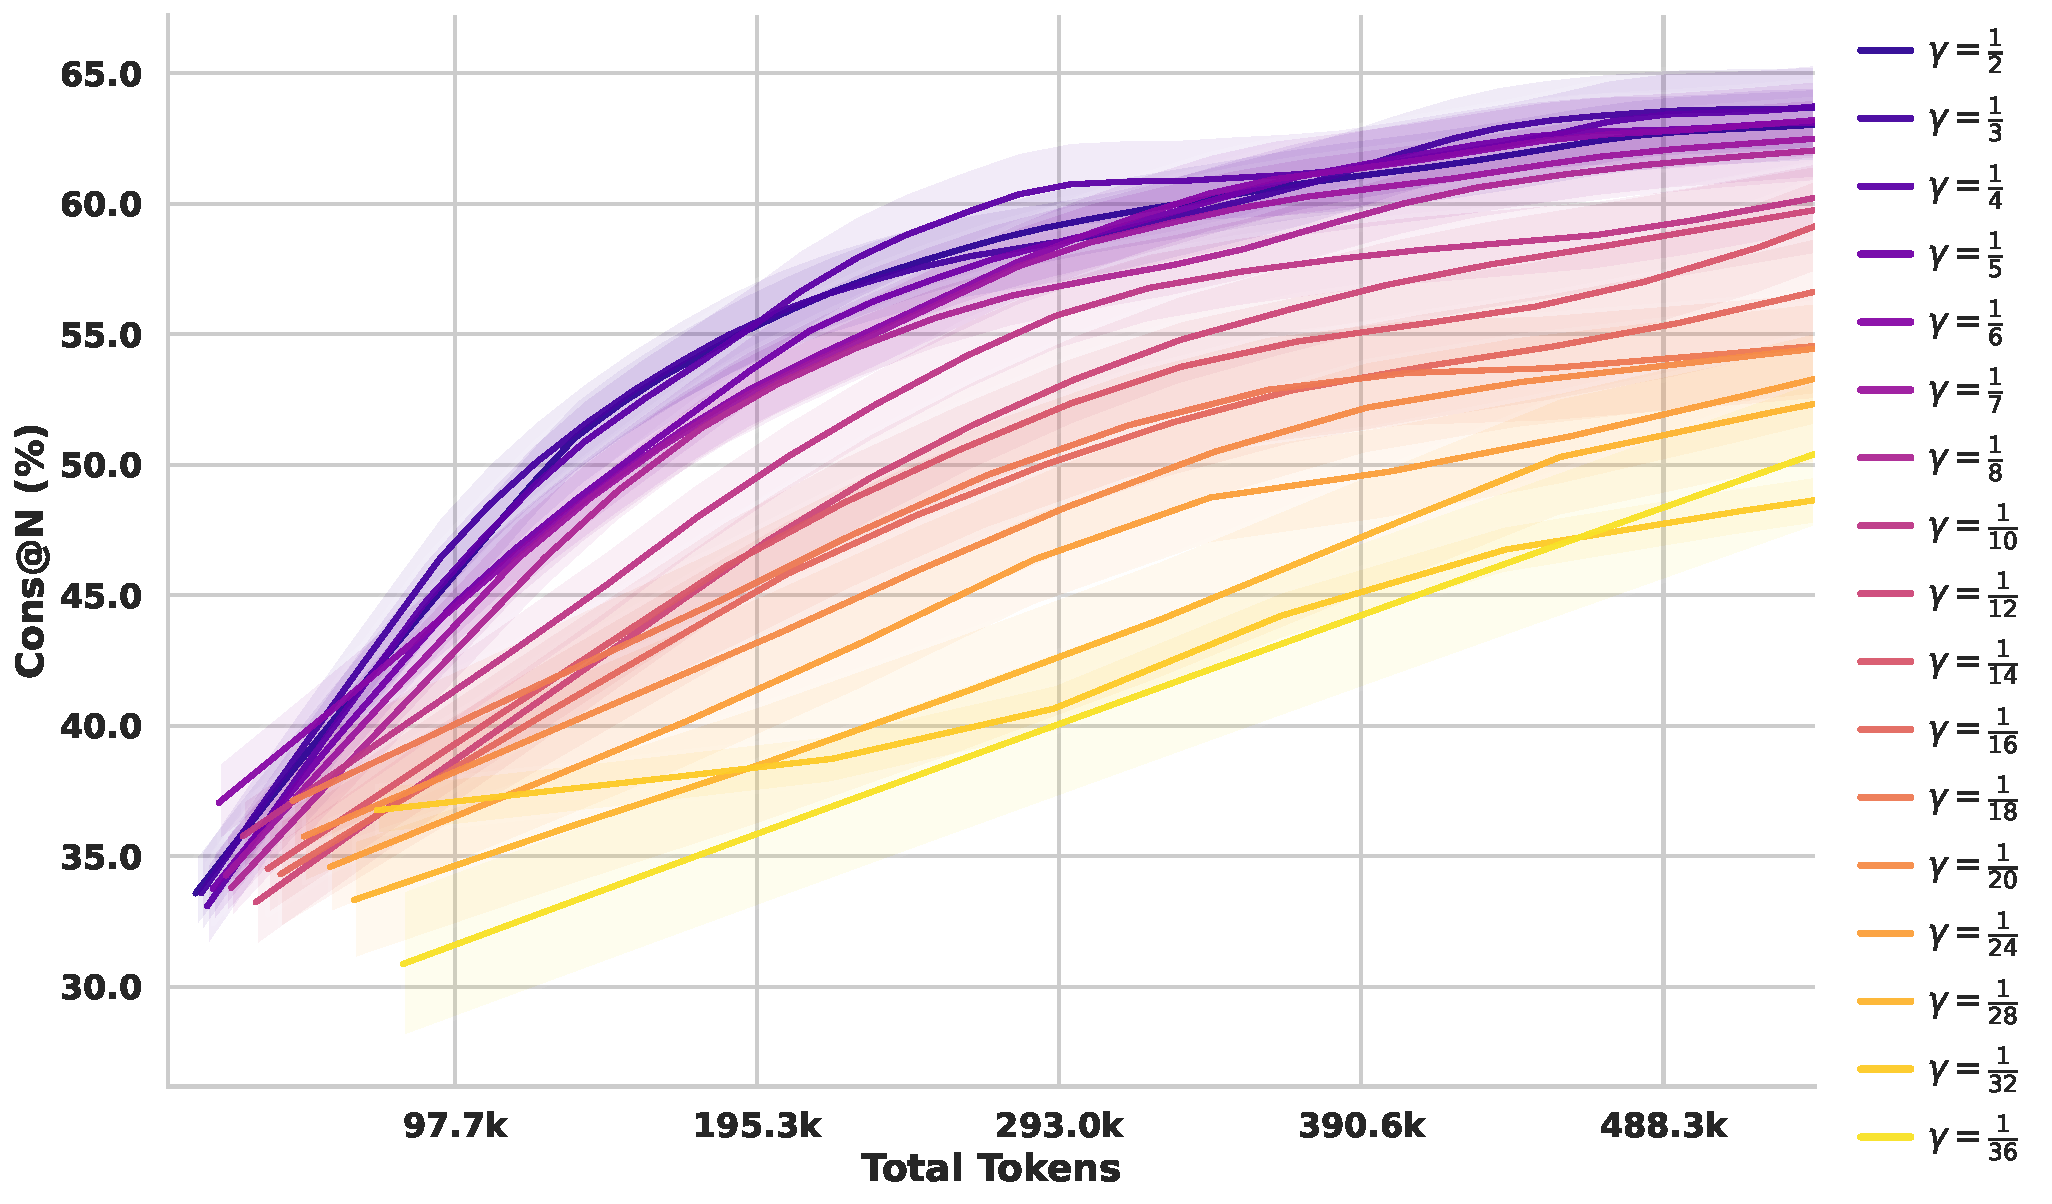
\includegraphics[height=5.0cm, keepaspectratio]{figures/Optimal_Pruning/1.5B_aime_2048.pdf}
%     \caption{\textbf{AIME 2024 ($L_{prefix}=2048$)}. Optimal $\gamma$ shifts to aggressive pruning as budget increases.}
%     \label{fig:fit_aime_2048}
%   \end{subfigure}
%   \hfill
%   \begin{subfigure}[b]{0.45\linewidth}
%     \centering
%     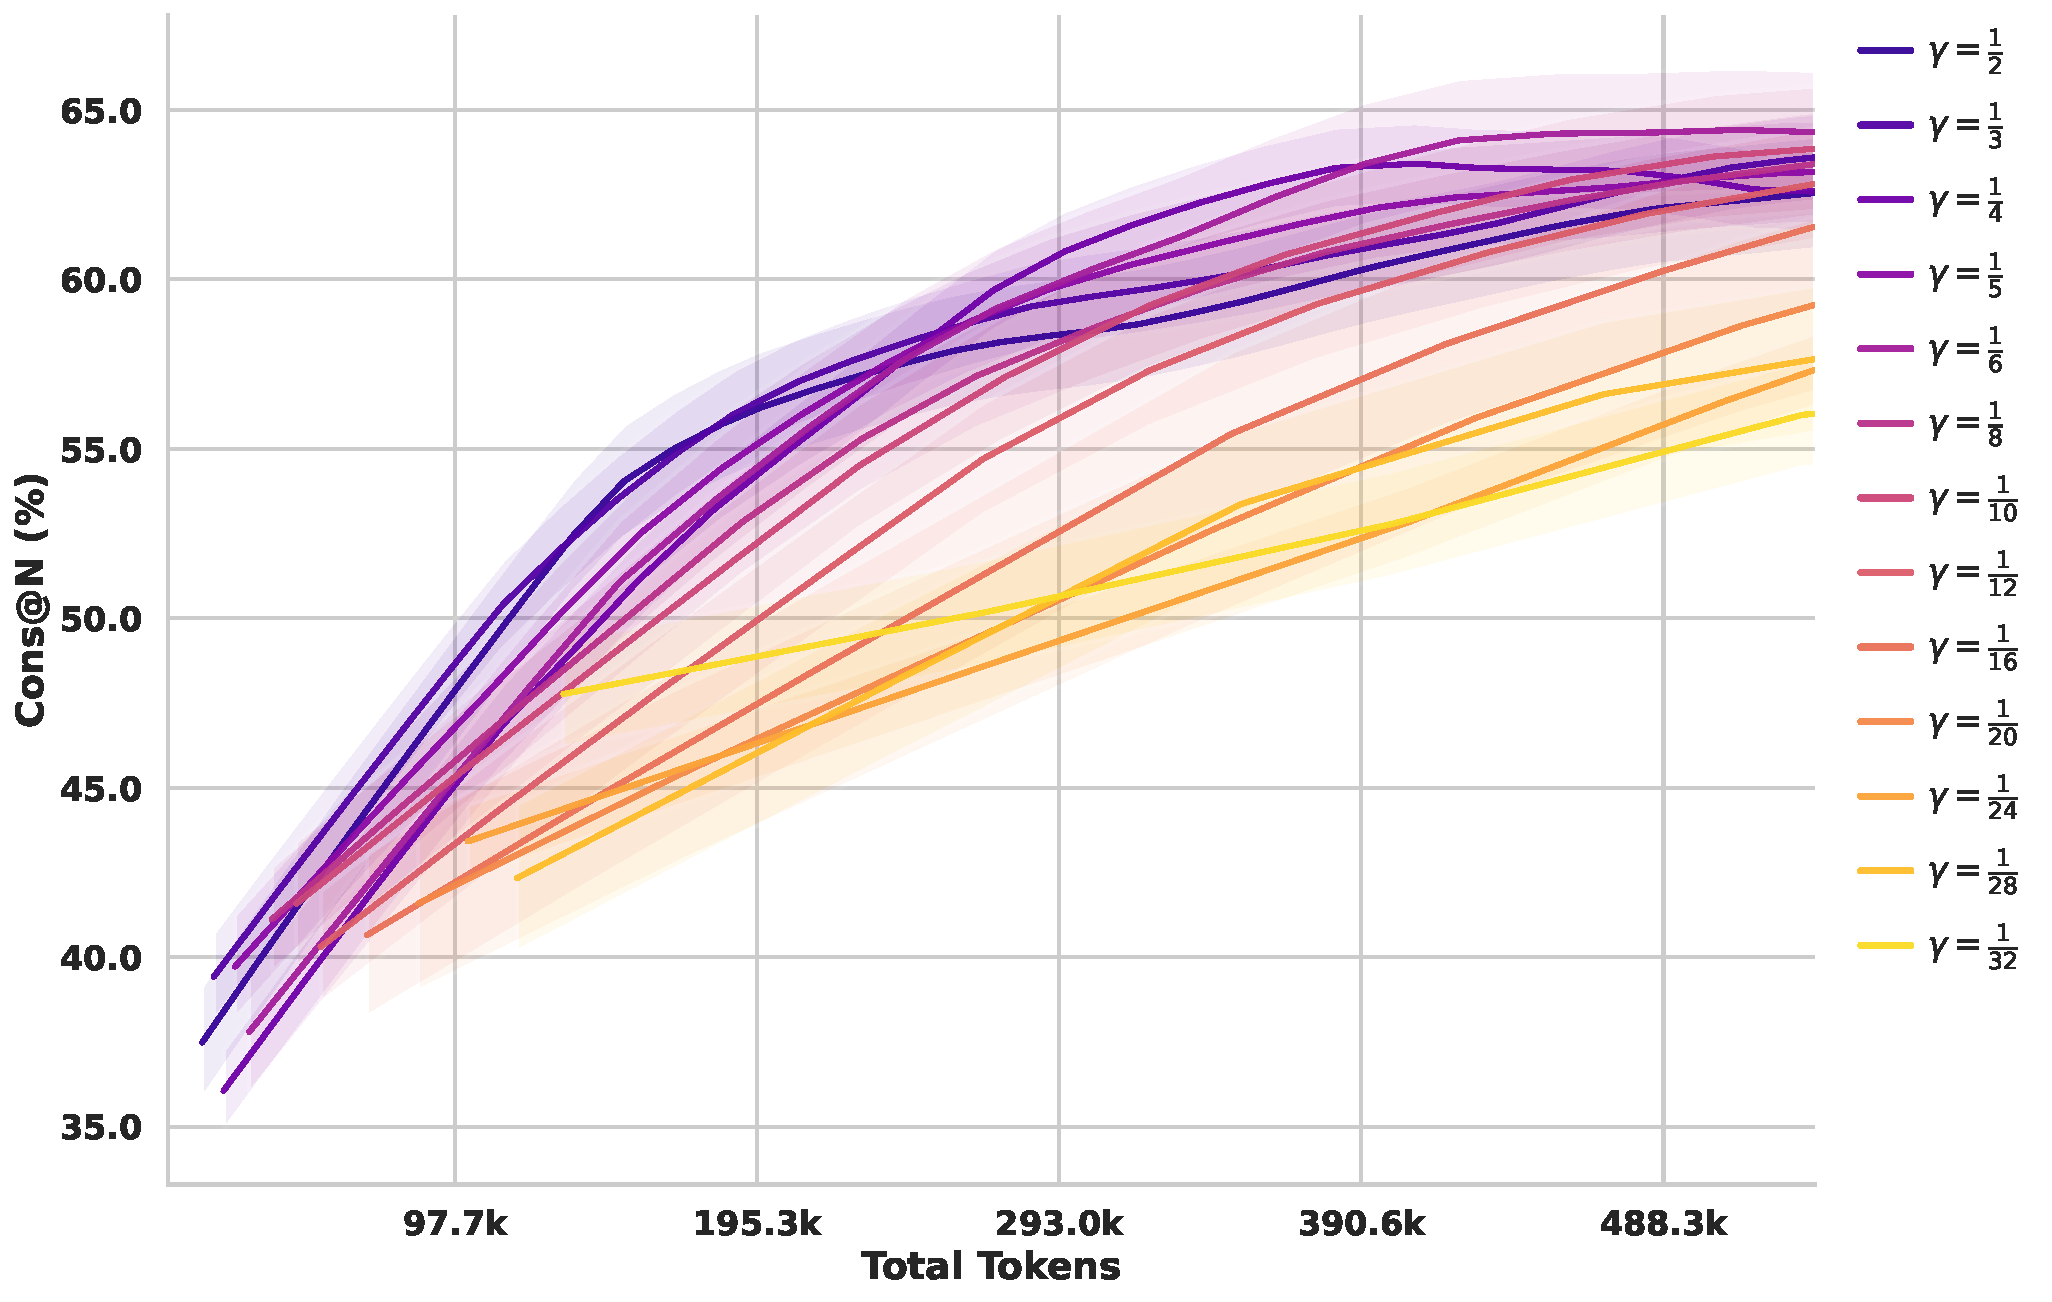
\includegraphics[height=5.0cm, keepaspectratio]{figures/Optimal_Pruning/1.5B_aime_4096.pdf} 
%     \caption{\textbf{AIME 2024 ($L_{prefix}=4096$)}. Longer context enables stable pruning at higher selectivity.}
%     \label{fig:fit_aime_4096}
%   \end{subfigure}
  
%   \vspace{1em}
  
% % --- Row 2: GPQA (Science) ---
%   \begin{subfigure}[b]{0.45\linewidth}
%     \centering
%     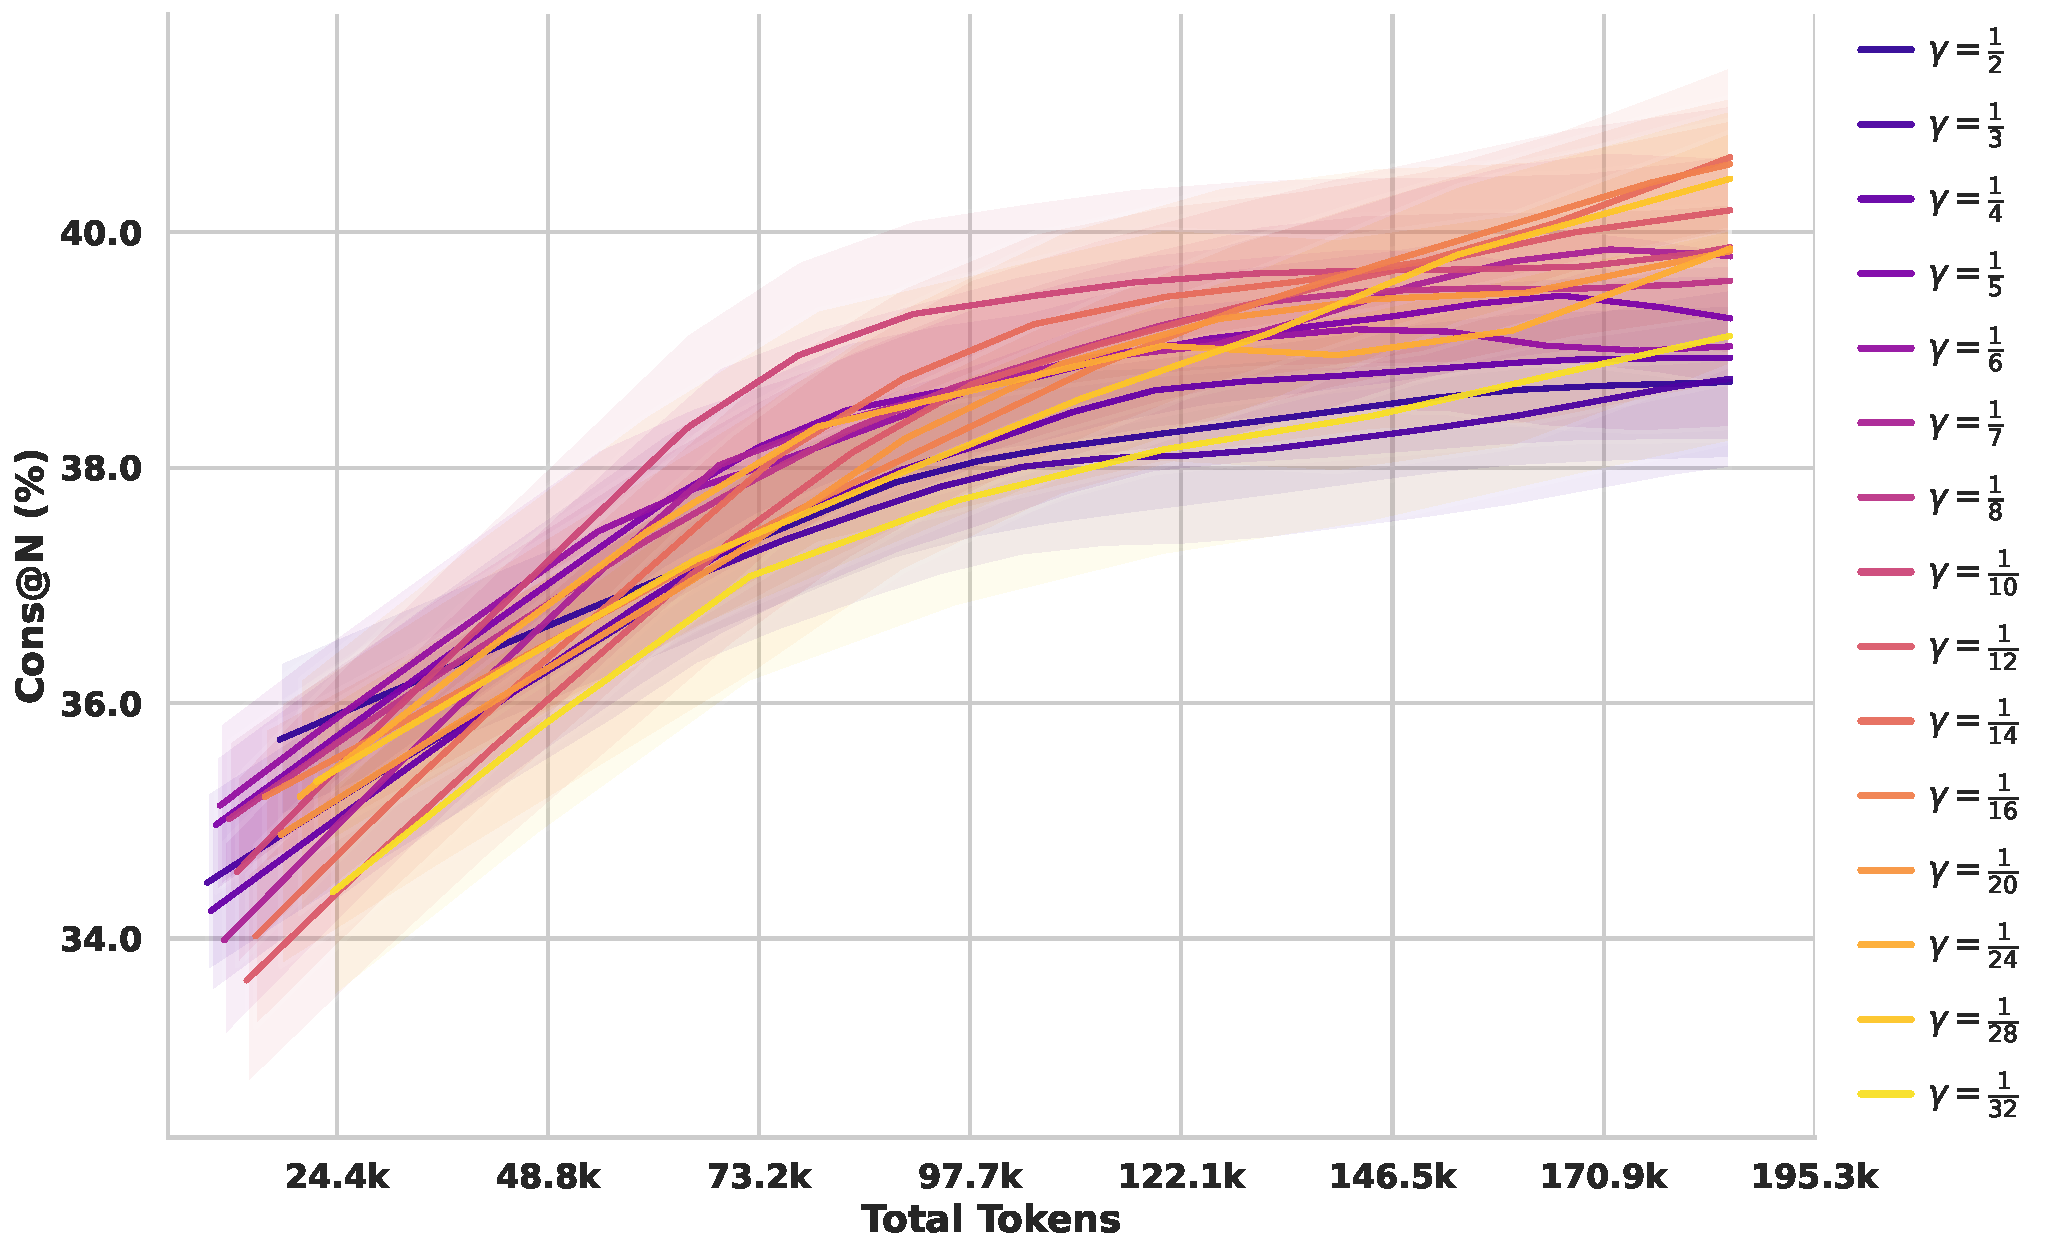
\includegraphics[height=5.0cm, keepaspectratio]{figures/Optimal_Pruning/1.5B_gpqa_512.pdf}
%     \caption{\textbf{GPQA ($L_{prefix}=512$)}. Higher compute budgets drive the optimal strategy towards more aggressive pruning.}
%     \label{fig:fit_gpqa_512}
%   \end{subfigure}
%   \hfill
%   \begin{subfigure}[b]{0.45\linewidth}
%     \centering
%     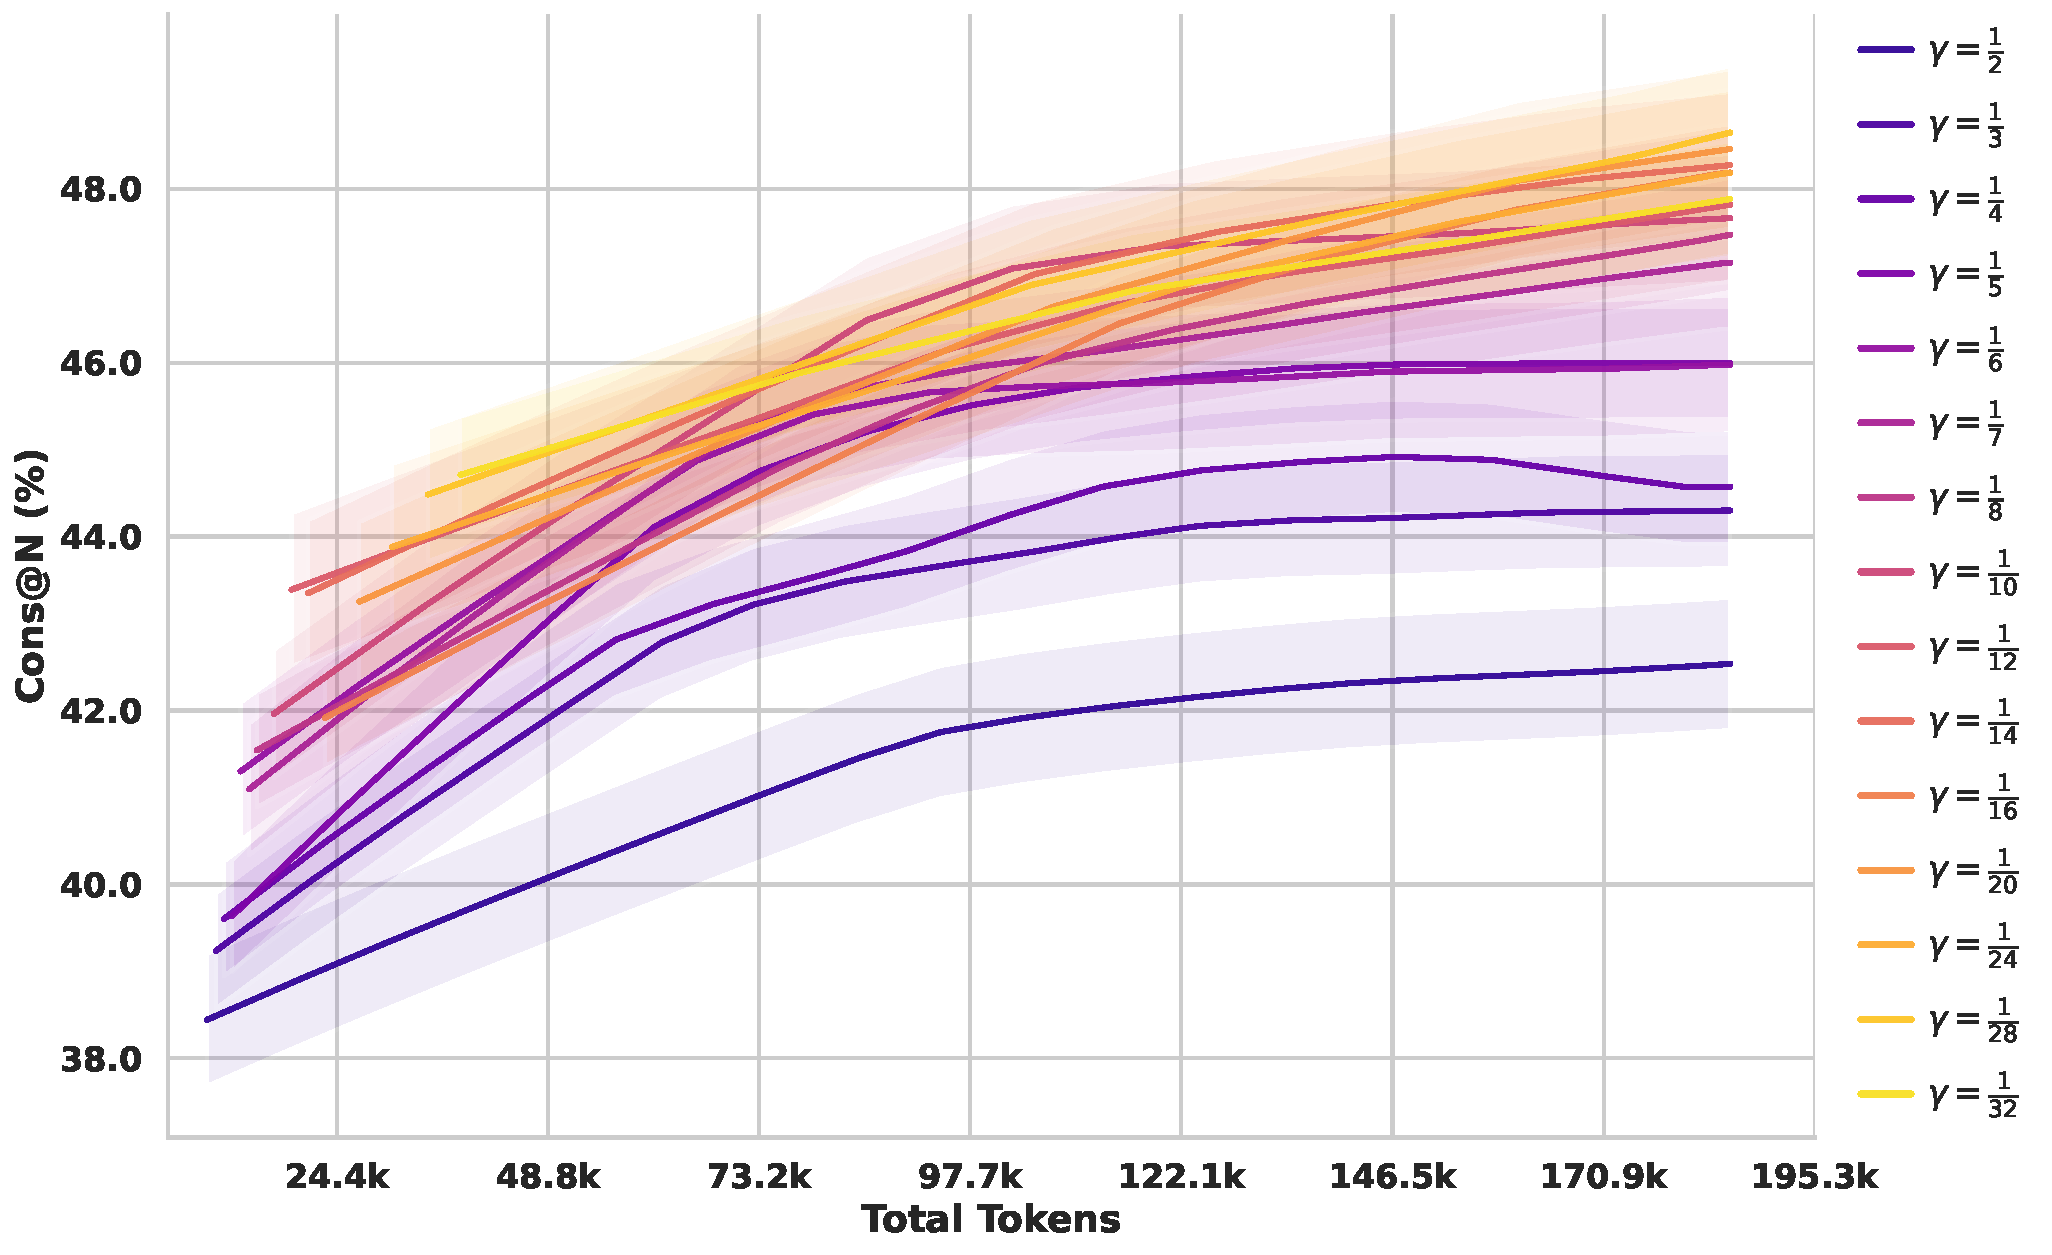
\includegraphics[height=5.0cm, keepaspectratio]{figures/Optimal_Pruning/1.5B_gpqa_1024.pdf} 
%     \caption{\textbf{GPQA ($L_{prefix}=1024$)}. This scaling behavior remains consistent even with extended context windows.}
%     \label{fig:fit_gpqa_1024}
%   \end{subfigure}
  
%   \caption{\textbf{Empirical Optimization Surfaces.} We visualize the impact of varying the retention ratio $\gamma$ (represented by different curves) across increasing compute budgets.}
%   \label{fig:scaling_raw_data} 
% \vspace{-4mm}
% \end{figure*}
\begin{figure*}[t]
\vspace{-6mm}
  \centering

  % --- Row 1 ---
  \begin{subfigure}[b]{0.45\linewidth}
    \centering
    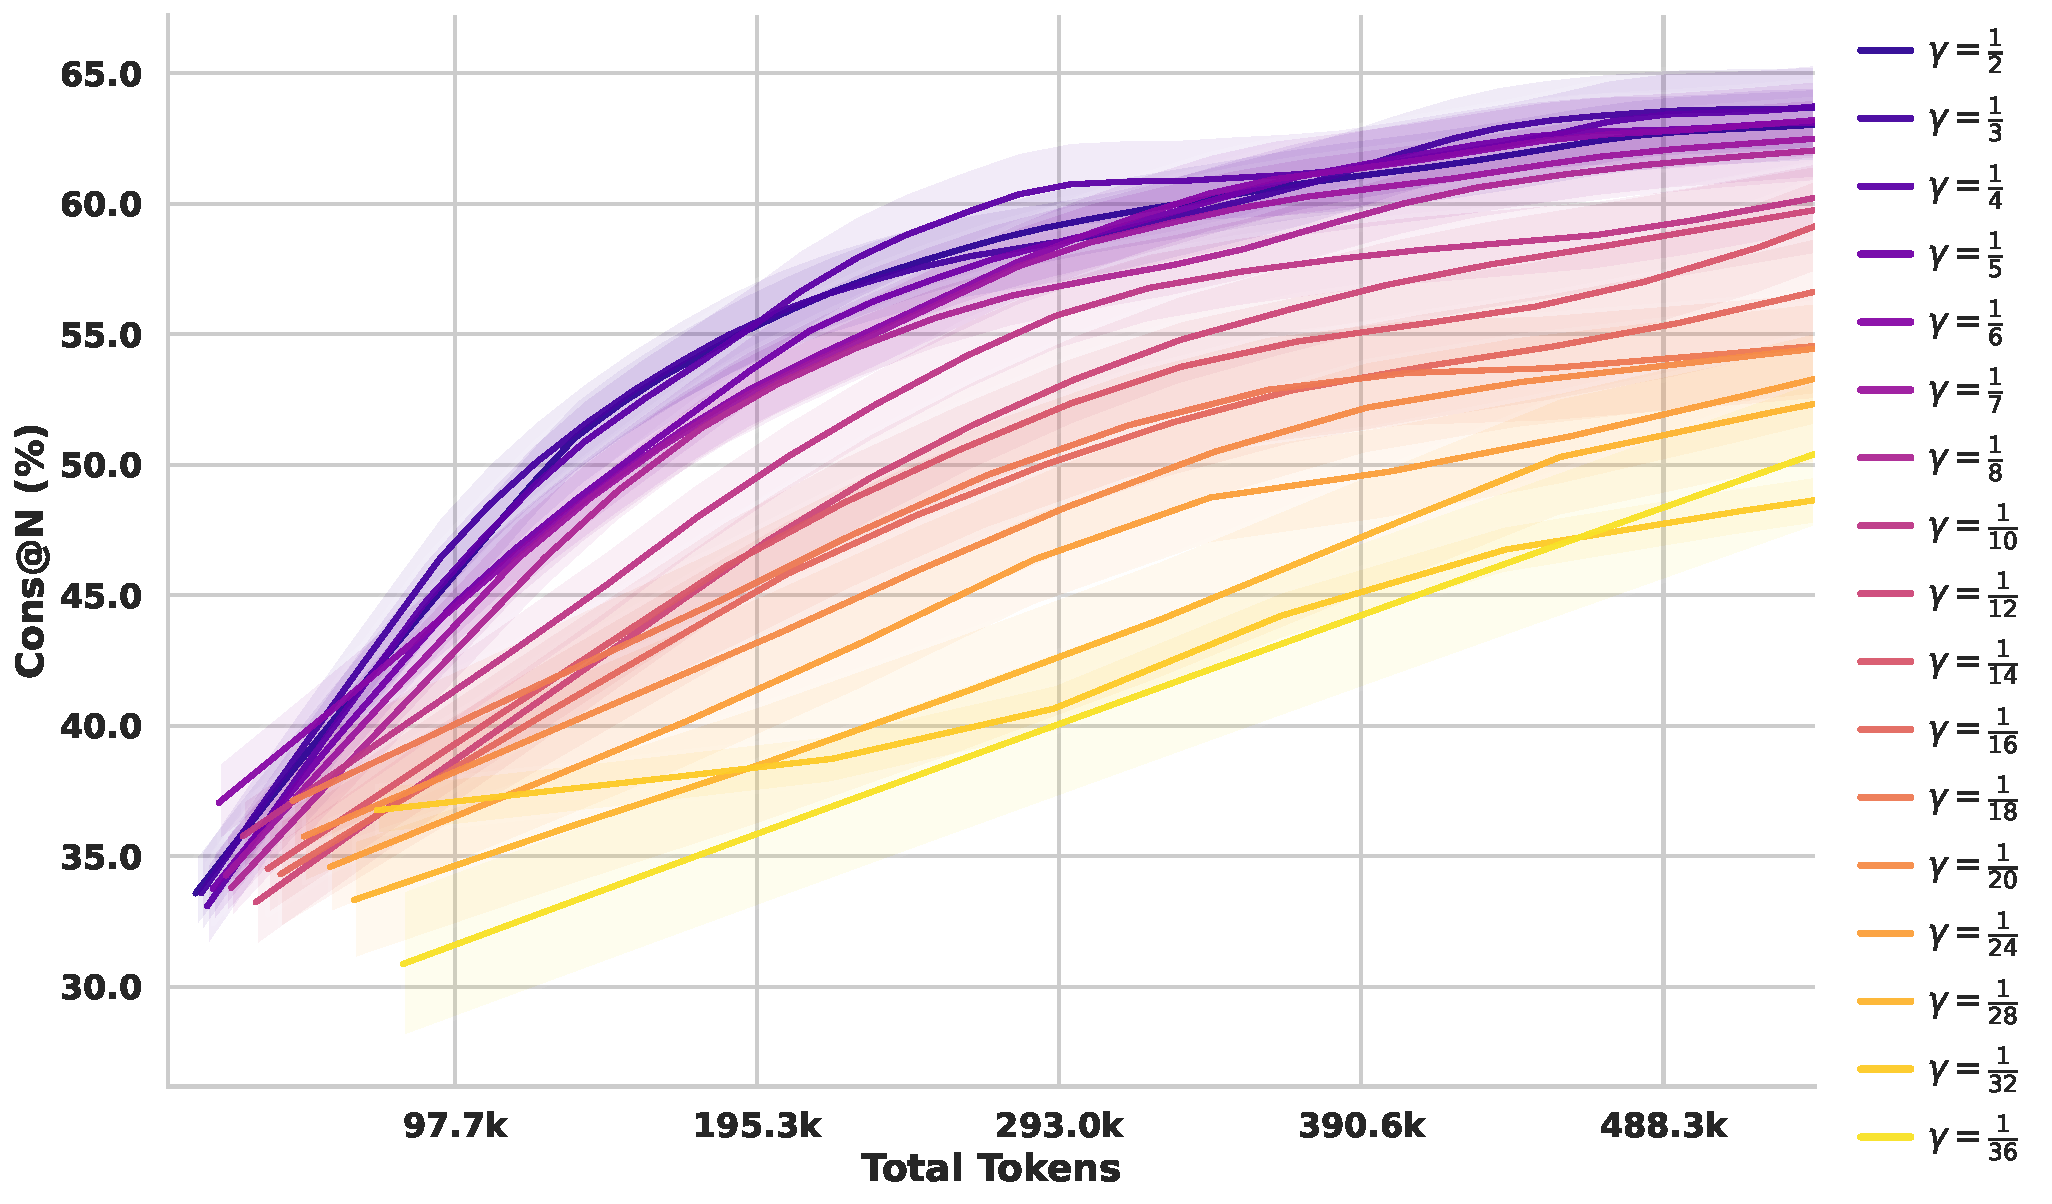
\includegraphics[height=4.2cm]{figures/Optimal_Pruning/1.5B_aime_2048.pdf}
    \caption{\textbf{AIME 2024 ($L_{prefix}=2048$)}. Optimal $\gamma$ shifts to aggressive pruning as budget increases.}
  \end{subfigure}
  \hfill
  \begin{subfigure}[b]{0.45\linewidth}
    \centering
    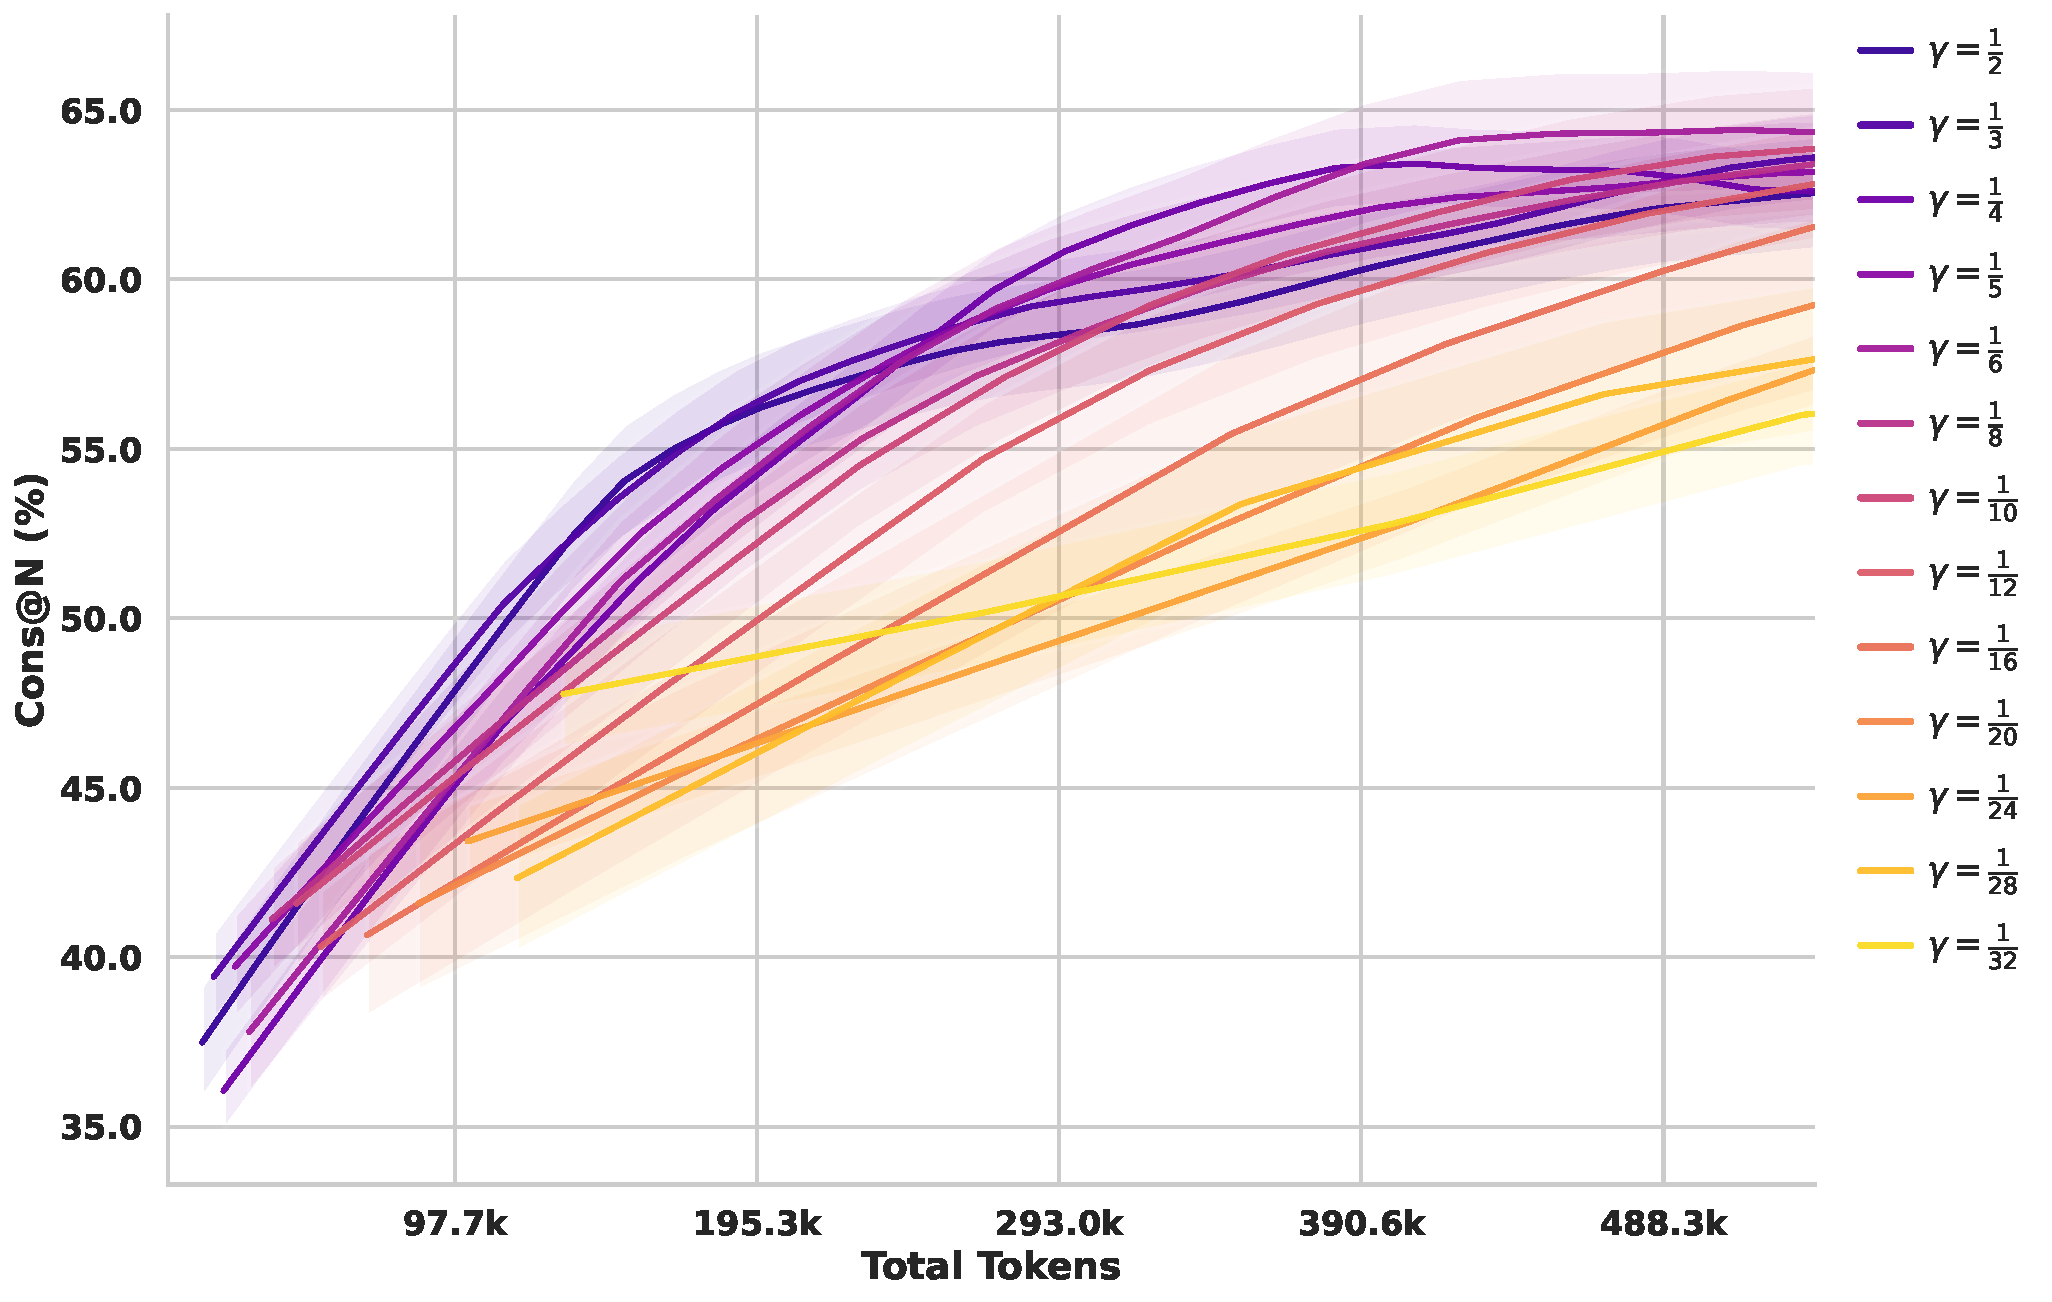
\includegraphics[height=4.2cm]{figures/Optimal_Pruning/1.5B_aime_4096.pdf}
    \caption{\textbf{AIME 2024 ($L_{prefix}=4096$)}. Longer context enables stable pruning at higher selectivity.}
  \end{subfigure}

  \vspace{0.6em}

  % --- Row 2 ---
  \begin{subfigure}[b]{0.45\linewidth}
    \centering
    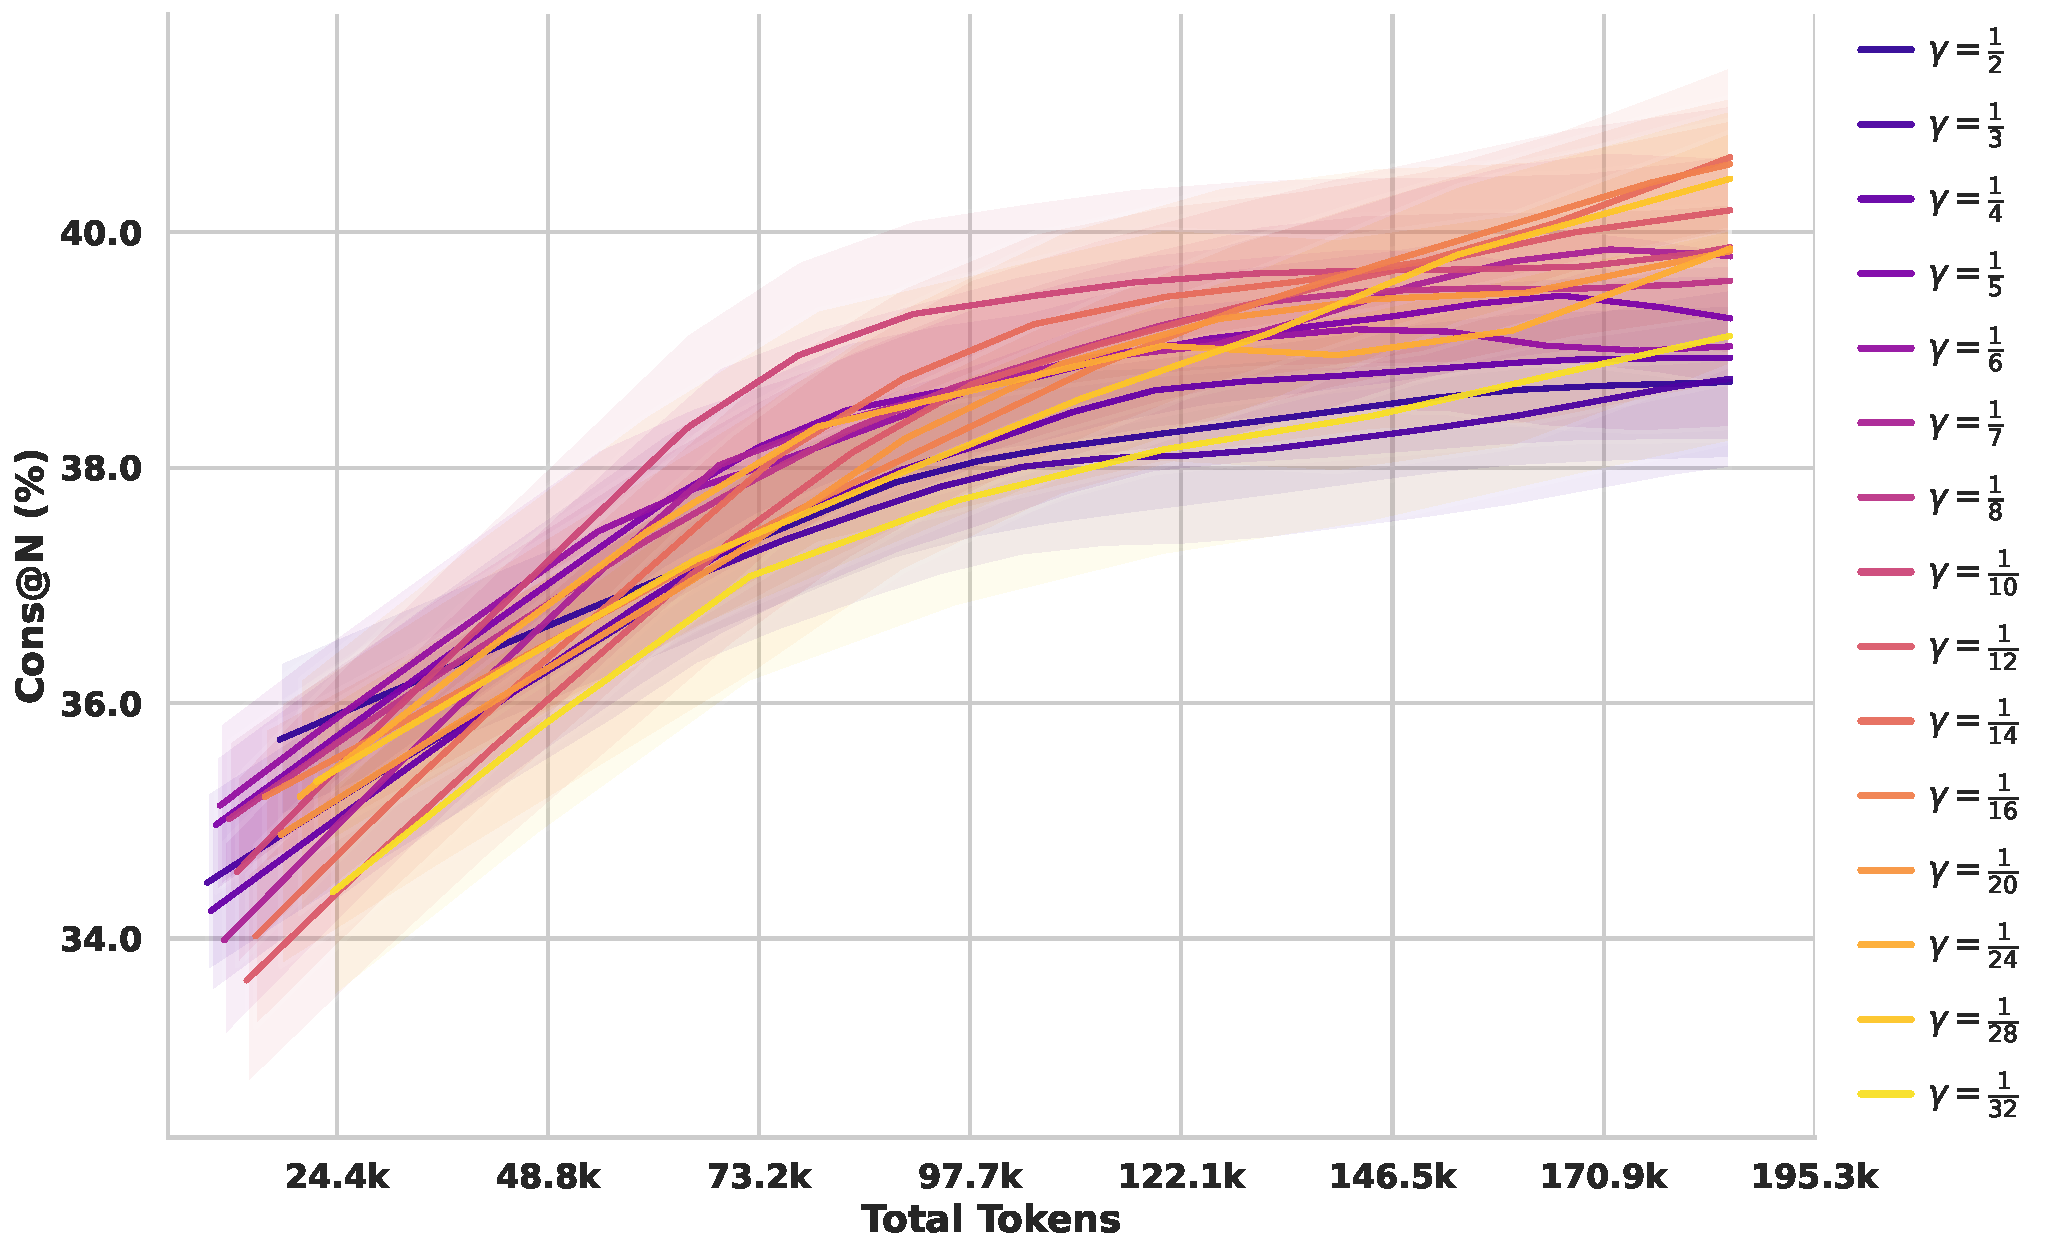
\includegraphics[height=4.2cm]{figures/Optimal_Pruning/1.5B_gpqa_512.pdf}
    \caption{\textbf{GPQA ($L_{prefix}=512$)}. Higher compute budgets drive more aggressive pruning.}
  \end{subfigure}
  \hfill
  \begin{subfigure}[b]{0.45\linewidth}
    \centering
    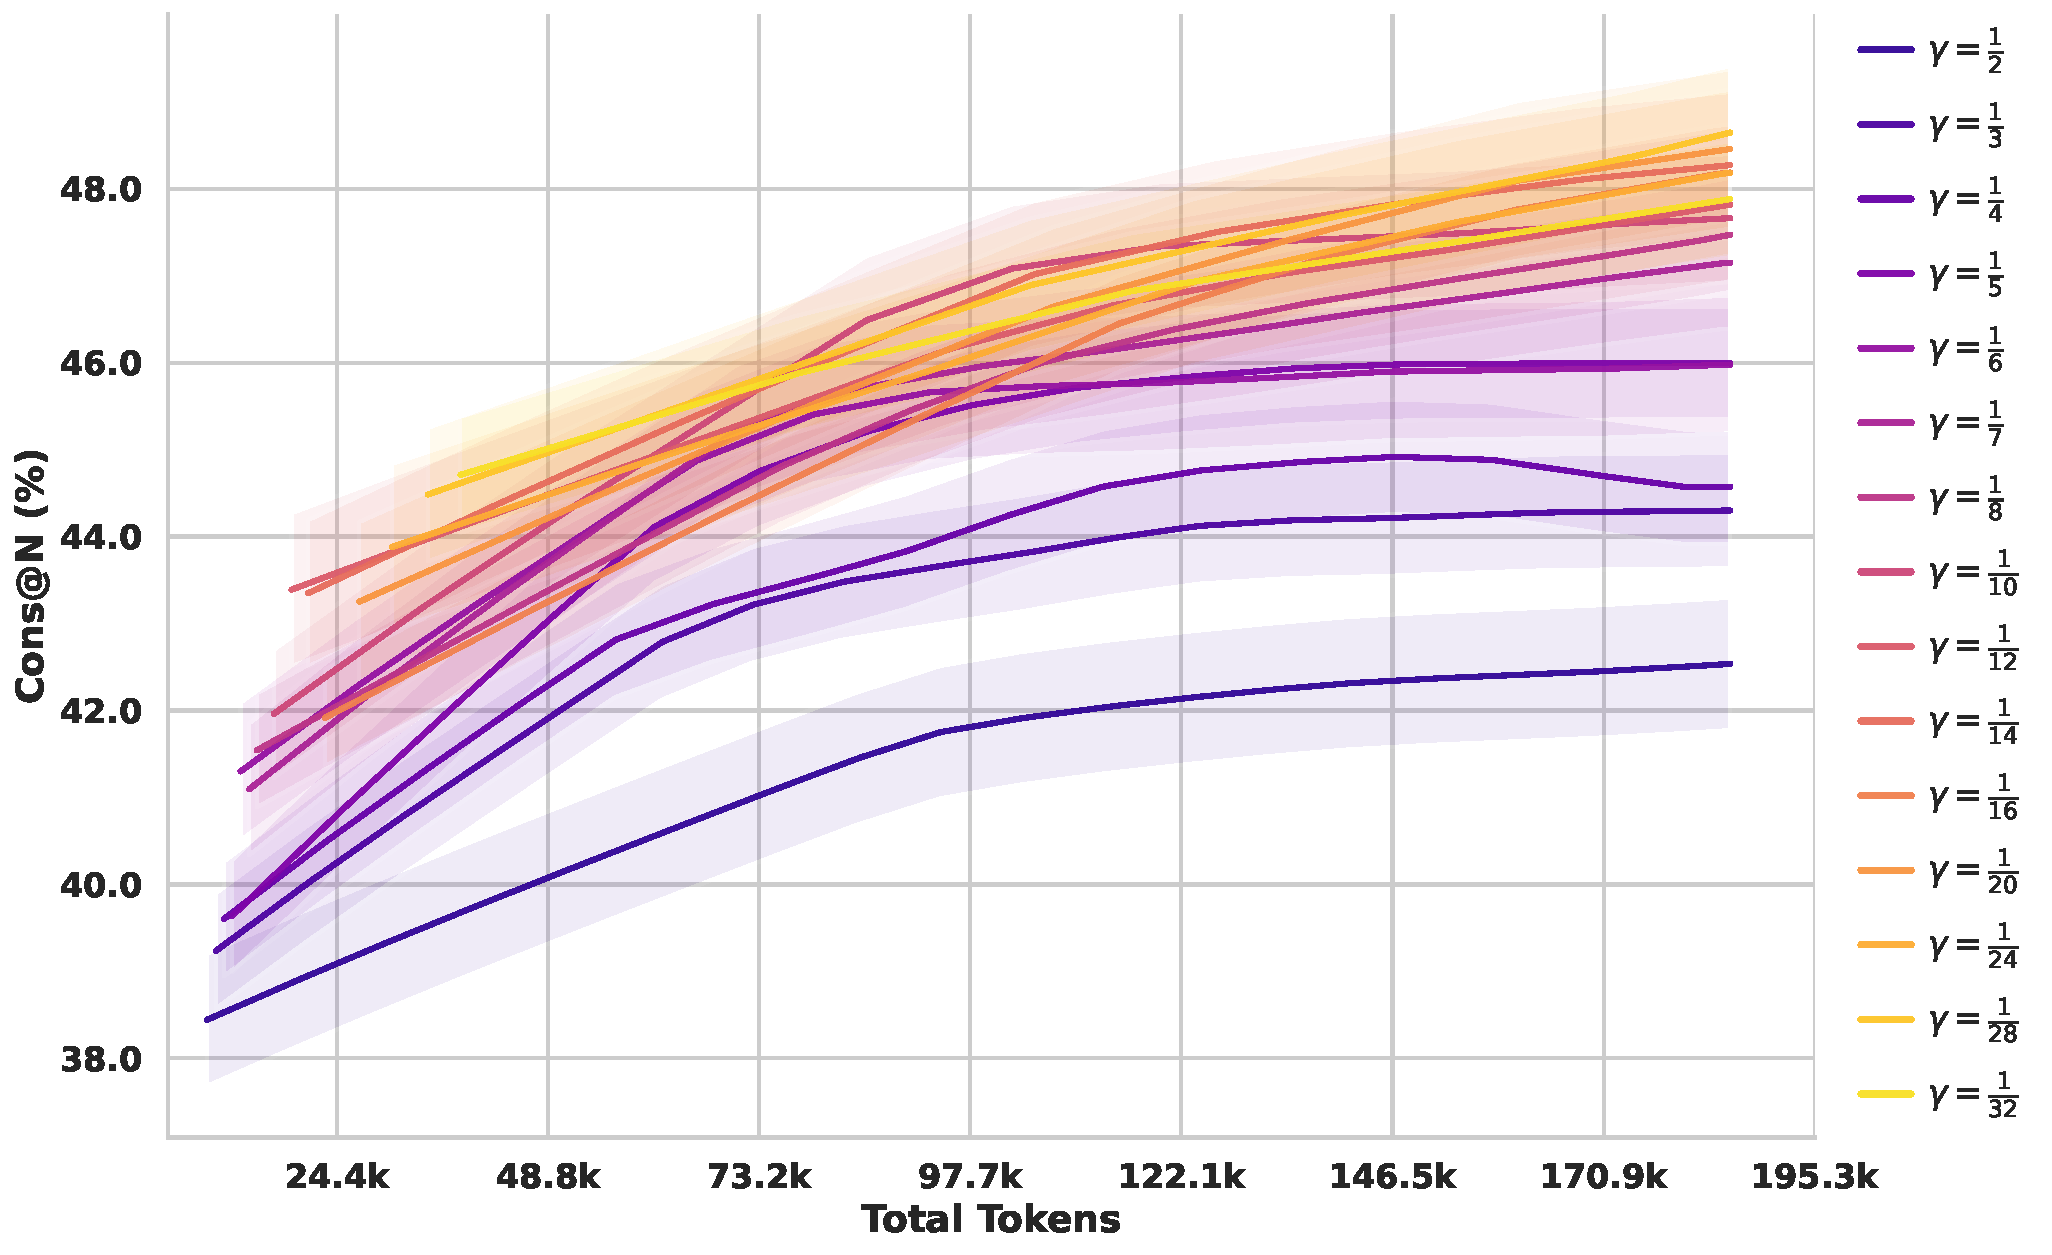
\includegraphics[height=4.2cm]{figures/Optimal_Pruning/1.5B_gpqa_1024.pdf}
    \caption{\textbf{GPQA ($L_{prefix}=1024$)}. Scaling behavior remains consistent with longer contexts.}
  \end{subfigure}

  \caption{\textbf{Empirical optimization surfaces.} Impact of retention ratio $\gamma$ across increasing compute budgets.}
  \label{fig:scaling_raw_data}
% \vspace{-5mm}
\end{figure*}

\begin{table*}[t]
% \vspace{-4mm}
    \centering
    \small
    \setlength{\tabcolsep}{5pt}
    \caption{\textbf{GPQA (Science, Short-Horizon).} Recommended inverse retention ratios ($\gamma^{-1}$) for tasks with shorter reference lengths ($L_{\text{task}} \approx 8{,}650$). Pruning is more aggressive (higher values) even at lower budgets.}
    \label{tab:gamma_lookup_gpqa}
    \begin{tabular}{c ccccccccc}
    \toprule
    \multirow{2}{*}{\textbf{Prefix Length}} & \multicolumn{9}{c}{\textbf{Compute Budget $C$ (Total Tokens)}} \\
    \cmidrule(lr){2-10}
    ($L_{\text{prefix}}$) & \textbf{140k} & \textbf{160k} & \textbf{180k} & \textbf{200k} & \textbf{220k} & \textbf{240k} & \textbf{260k} & \textbf{280k} & \textbf{300k} \\
    \midrule
    512   & 5.23 & 5.56 & 5.87 & 6.16 & 6.44 & 6.70 & 6.95 & 7.19 & 7.42 \\
    1024  & 6.90 & 7.34 & 7.75 & 8.13 & 8.49 & 8.84 & 9.17 & 9.49 & 9.80 \\
    1536  & 8.11 & 8.63 & 9.11 & 9.56 & 9.99 & 10.40 & 10.79 & 11.16 & 11.52 \\
    2048  & 9.10 & 9.68 & 10.22 & 10.73 & 11.21 & 11.67 & 12.10 & 12.52 & 12.93 \\
    2560  & 9.95 & 10.59 & 11.17 & 11.73 & 12.26 & 12.76 & 13.23 & 13.69 & 14.13 \\
    \bottomrule
    \end{tabular}
\end{table*}

\begin{table*}[t]
    \centering
    \small
    \setlength{\tabcolsep}{5pt}
    \caption{\textbf{AIME (Math, Long-Horizon).} Recommended inverse retention ratios ($\gamma^{-1}$) for tasks with longer reference lengths ($L_{\text{task}} \approx 11{,}950$). Pruning is more conservative (lower values) due to higher reasoning complexity.}
    \label{tab:gamma_lookup_aime}
    \begin{tabular}{c ccccccccc}
    \toprule
    \multirow{2}{*}{\textbf{Prefix Length}} & \multicolumn{9}{c}{\textbf{Compute Budget $C$ (Total Tokens)}} \\
    \cmidrule(lr){2-10}
    ($L_{\text{prefix}}$) & \textbf{200k} & \textbf{250k} & \textbf{300k} & \textbf{350k} & \textbf{400k} & \textbf{450k} & \textbf{500k} & \textbf{550k} & \textbf{600k} \\
    \midrule
    1024  & 1.87 & 2.07 & 2.25 & 2.42 & 2.57 & 2.71 & 2.85 & 2.98 & 3.10 \\
    2048  & 2.47 & 2.73 & 2.97 & 3.19 & 3.39 & 3.58 & 3.76 & 3.93 & 4.09 \\
    3072  & 2.90 & 3.21 & 3.49 & 3.75 & 3.99 & 4.21 & 4.42 & 4.62 & 4.81 \\
    4096  & 3.25 & 3.60 & 3.92 & 4.21 & 4.48 & 4.72 & 4.96 & 5.18 & 5.39 \\
    5120  & 3.56 & 3.94 & 4.29 & 4.60 & 4.89 & 5.17 & 5.42 & 5.66 & 5.90 \\
    \bottomrule
    \end{tabular}
\end{table*}


\subsection{Recommended Retention Guidelines}
\label{app:gamma_guidelines}

Based on the derived scaling law, we provide reference tables for selecting optimal pruning strategies. To \textbf{improve visual clarity and facilitate quick lookup}, we present the guidelines in two separate tables, each corresponding to a different compute budget regime.

These tables are intended primarily as \textbf{illustrative references} for representative task lengths. For other tasks, whether they are similar to GPQA or Math and have different response characteristics, practitioners can directly substitute the task length ($L_{task}$), prefix length ($L_{prefix}$), and compute budget ($C$) into the derived formula (Eq.~\ref{eq:optimial_gamma}) to obtain the exact optimal retention ratio.

Tables~\ref{tab:gamma_lookup_gpqa} and~\ref{tab:gamma_lookup_aime} report the recommended \textbf{inverse retention ratio} ($\gamma^{-1}$) for representative short-horizon tasks ($L_{task} \approx 8{,}650$) and long-horizon tasks ($L_{task} \approx 11{,}950$), respectively.

% \begin{table}[H]
%     \centering
%     \caption{\textbf{GPQA (Science, Short-Horizon).} Recommended Inverse Retention Ratios ($\gamma^{-1}$) for tasks with shorter reference lengths ($L_{task} \approx 8,650$). Pruning is more aggressive (higher values) even at lower budgets.}
%     \label{tab:gamma_lookup_gpqa}
%     \begin{tabular}{cccccccccc}
%     \toprule
%     \multirow{2}{*}{\textbf{Prefix Length}} & \multicolumn{9}{c}{\textbf{Compute Budget $C$ (Total Tokens)}} \\
%     \cmidrule(lr){2-10}
%     ($L_{prefix}$) & \textbf{140k} & \textbf{160k} & \textbf{180k} & \textbf{200k} & \textbf{220k} & \textbf{240k} & \textbf{260k} & \textbf{280k} & \textbf{300k} \\
%     \midrule
%     512   & 5.23 & 5.56 & 5.87 & 6.16 & 6.44 & 6.70 & 6.95 & 7.19 & 7.42 \\
%     1024  & 6.90 & 7.34 & 7.75 & 8.13 & 8.49 & 8.84 & 9.17 & 9.49 & 9.80 \\
%     1536  & 8.11 & 8.63 & 9.11 & 9.56 & 9.99 & 10.40 & 10.79 & 11.16 & 11.52 \\
%     2048  & 9.10 & 9.68 & 10.22 & 10.73 & 11.21 & 11.67 & 12.10 & 12.52 & 12.93 \\
%     2560  & 9.95 & 10.59 & 11.17 & 11.73 & 12.26 & 12.76 & 13.23 & 13.69 & 14.13 \\
%     \bottomrule
%     \end{tabular}
    
%     \vspace{0.5cm}
    
%     \caption{\textbf{AIME (Math, Long-Horizon).} Recommended Inverse Retention Ratios ($\gamma^{-1}$) for tasks with longer reference lengths ($L_{task} \approx 11,950$). Pruning is more conservative (lower values) due to higher reasoning complexity.}
%     \label{tab:gamma_lookup_aime}
%     \begin{tabular}{cccccccccc}
%     \toprule
%     \multirow{2}{*}{\textbf{Prefix Length}} & \multicolumn{9}{c}{\textbf{Compute Budget $C$ (Total Tokens)}} \\
%     \cmidrule(lr){2-10}
%     ($L_{prefix}$) & \textbf{200k} & \textbf{250k} & \textbf{300k} & \textbf{350k} & \textbf{400k} & \textbf{450k} & \textbf{500k} & \textbf{550k} & \textbf{600k} \\
%     \midrule
%     1024  & 1.87 & 2.07 & 2.25 & 2.42 & 2.57 & 2.71 & 2.85 & 2.98 & 3.10 \\
%     2048  & 2.47 & 2.73 & 2.97 & 3.19 & 3.39 & 3.58 & 3.76 & 3.93 & 4.09 \\
%     3072  & 2.90 & 3.21 & 3.49 & 3.75 & 3.99 & 4.21 & 4.42 & 4.62 & 4.81 \\
%     4096  & 3.25 & 3.60 & 3.92 & 4.21 & 4.48 & 4.72 & 4.96 & 5.18 & 5.39 \\
%     5120  & 3.56 & 3.94 & 4.29 & 4.60 & 4.89 & 5.17 & 5.42 & 5.66 & 5.90 \\
%     \bottomrule
%     \end{tabular}
% \end{table}


\section{Detailed Latency and Throughput Benchmarking}
\label{app:latency_details}

In this appendix, we present a detailed analysis of the system efficiency discussed in Section~\ref{subsec:ablation}.
We conduct controlled micro-benchmarks on a single NVIDIA H100 GPU using \textbf{DS-Qwen-2.5-7B}.
The evaluation uses a batch size of 16 and a fixed prefix length of 2,048 tokens to simulate realistic inference conditions.

\subsection{Metric Definitions}
We adopt the following metrics to evaluate computational overhead:
\begin{itemize}[leftmargin=*, noitemsep, topsep=0pt]
    \item \textbf{Generation Time ($T_{\text{gen}}$):} The wall-clock time required for autoregressive decoding of reasoning tokens, excluding any verification operations.
    \item \textbf{Verification Latency ($T_{\text{verify}}$):} The explicit computation time required by the pruning signal generator to produce scores for a batch.
    \item \textbf{System Throughput:} The effective inference speed measured in tokens per second (tok/s). Unlike latency metrics, throughput captures implicit system-level overheads, including CPU--GPU synchronization and pipeline inefficiencies caused by context switching.
\end{itemize}

\subsection{Quantitative Analysis}
Table~\ref{tab:detailed_latency} reports the detailed timing breakdown across different pruning paradigms.
The results reveal a clear mismatch between explicit verification latency and the realized system throughput, especially for heuristic-based methods.

% \begin{table*}[t!]
% \centering
% \small
% \caption{\textbf{Breakdown of Inference Latency and Throughput.} Although $S_{\text{heuristic}}$ (SlimSC) exhibits a low explicit verification latency (0.38s), frequent interruptions significantly increase the total generation time, resulting in an approximately 17\% throughput degradation. As a result, its reported relative overhead (1.74\%) underestimates the true system cost. In contrast, \textsc{STOP} maintains high throughput (960.1 tok/s) with negligible overhead (0.59\%).}
% \label{tab:detailed_latency}
% \begin{tabular}{l c c c c c}
% \toprule
% \textbf{Method} & \textbf{Gen. Time (s)} & \textbf{Verify Latency (s)} & \textbf{Total Time (s)} & \textbf{Throughput (tok/s)} & \textbf{Relative Overhead} \\
% \midrule
% \textbf{Baseline} (No Pruning) & 33.20 & -- & 33.20 & 986.9 & -- \\
% \midrule
% $S_{\text{aux}}$ (External PRM) & 33.53 & 1.13 & 34.68 & 977.3 & 3.37\% \\
% $S_{\text{heuristic}}$ (SlimSC) & 40.64 & 0.38 & 41.02 & 812.1 & 1.74\% \\
% $S_{\text{module}}$ (\textbf{STOP}) & 34.13 & \textbf{0.20} & 34.33 & \textbf{960.1} & \textbf{0.59\%} \\
% \bottomrule
% \end{tabular}
% \end{table*}
\begin{table*}[t!]
\centering
\small
\caption{\textbf{Breakdown of Inference Latency and Throughput.} 
Note the discrepancy between \textit{explicit cost} and \textit{system impact} for heuristic methods. 
Although Type~\ref{type:heuristic} (SlimSC) shows a low explicit verification cost (1.74\%), the pipeline fragmentation significantly slows down generation, causing a massive \textbf{17.71\% drop in throughput}. 
In contrast, \textsc{STOP} operates in-situ, keeping the throughput drop minimal ($<3\%$) with negligible verification cost (0.59\%).}
\label{tab:detailed_latency}
\resizebox{0.95\linewidth}{!}{
\begin{tabular}{l c c c c c c}
\toprule
\textbf{Method} & \textbf{Gen. Time (s)} & \textbf{Verify Latency (s)} & \textbf{Total Time (s)} & \textbf{Throughput (tok/s)} & \textbf{Throughput Drop ($\downarrow$)} & \textbf{Explicit Verify Cost} \\
\midrule
\textbf{Baseline} (No Pruning) & 33.20 & -- & 33.20 & 986.9 & -- & -- \\
\midrule
Type~\ref{type:heuristic} (SlimSC) & 40.64 & 0.38 & 41.02 & 812.1 & \textbf{17.71\%} & 1.74\% \\
Type~\ref{type:aux} (LaBoR) & 33.53 & 1.13 & 34.68 & 977.3 & 0.97\% & 3.37\% \\
Type~\ref{type:module} (\textbf{STOP}) & 34.13 & \textbf{0.20} & 34.33 & \textbf{960.1} & \textbf{2.71\%} & \textbf{0.59\%} \\
\bottomrule
\end{tabular}
}
\end{table*}


\noindent\textbf{Throughput degradation in heuristic methods.}
A key observation is the pronounced throughput drop in Type~\ref{type:heuristic} (SlimSC). 
Although the cumulative verification latency is small, the method requires frequent similarity computations during chunk-wise generation. 
These repeated interventions fragment GPU kernel execution, prevent sustained high utilization, and increase the base generation time from 33.20s to 40.64s.

\noindent\textbf{Efficiency and implementation of \textsc{STOP}.}
In contrast, the proposed \textsc{STOP} module introduces a minimal verification latency of 0.20s. 
By reusing the resident KV cache, \textsc{STOP} performs verification by processing the sequence $T_s$ in a single forward pass. 
During standard generation, the LoRA adapter remains disabled to strictly preserve the behavior of the base model and is activated only during the verification step. 
The prefix KV cache serves as a shared and immutable reference, and verification appends $T_s$ to a temporary view of this cache to compute the score. 
Once scoring is complete, the temporary branch is discarded. 
This design removes the need for context rollbacks or cache cleanup operations, ensuring that verification introduces no structural overhead into the generation pipeline. 
As a result, the total wall-clock time of \textsc{STOP} (34.33s) remains close to that of the baseline.

\noindent\textbf{Memory Footprint and Deployment Complexity.}
Beyond temporal latency, the spatial overhead of model deployment is a decisive factor.
Methods relying on external verifiers (Type~\ref{type:aux}) impose a \textbf{dual-model burden}: deploying Type~\ref{type:aux} (External PRM) requires hosting a separate PRM alongside the generator.
For example, using a 7B generator with a 7B reward model effectively doubles the VRAM requirement and increases orchestration complexity.
In contrast, \textsc{STOP} is implemented as a lightweight LoRA adapter attached directly to the frozen generator.
This \textbf{integrated architecture} adds only a minimal number of parameters, incurring \textbf{negligible additional VRAM overhead} for model weights.
It eliminates the need for managing secondary inference services, making \textsc{STOP} a "plug-and-play" solution for existing pipelines.

% \section{Derivation and Validation of the Scaling Law}
% \label{app:scaling_derivation}

% In Section~\ref{subsec:Power-law}, we introduce the Interaction Scaling Law to describe the relationship among the optimal pruning ratio $\gamma$, the compute budget $C$, and task complexity. Here, we further examine the empirical optimization surfaces that support this formulation.

% \subsection{Empirical Observations on Optimal Retention}
% We study how the optimal retention ratio $\gamma^*$, defined as the peak of the performance envelope under a fixed compute budget, varies across benchmarks and prefix lengths $L_{\text{prefix}}$.

% \noindent\textbf{Scientific Reasoning (GPQA).}
% For GPQA with $L_{\text{prefix}}=512$ and $1024$, the optimal strategy shifts toward more aggressive pruning as the compute budget increases. With short contexts ($L_{\text{prefix}}=512$), $\gamma^*$ is around $1/8$ at low budgets ($\sim 24$k tokens), reflecting a balance between exploration and exploitation. As the budget increases to $195$k tokens, the performance peak moves to smaller values ($\gamma \approx 1/16$), indicating that \textbf{STOP} effectively discards low-quality candidates when sufficient samples are available. For medium contexts ($L_{\text{prefix}}=1024$), conservative retention ($\gamma=1/2$) consistently underperforms. The optimal $\gamma^*$ starts near $1/8$ and rapidly decreases toward $\gamma \approx 1/28$ as compute increases.

% This pruning pattern arises from the concise reasoning structure of GPQA. GPQA solutions typically require few steps, so the fixed prefix captures a large portion of the full reasoning trajectory. As a result, the prefix contains high information density and provides a strong pruning signal, enabling \textbf{STOP} to aggressively filter candidates with low risk of removing correct solutions.

% \noindent\textbf{Mathematical Reasoning (AIME).}
% In contrast, AIME shows a strong dependence on prefix length, reflecting the higher sunk cost of long mathematical derivations. For $L_{\text{prefix}}=2048$, increasing the compute budget shifts the optimal $\gamma^*$ from conservative values ($\gamma \approx 1/2$) toward more aggressive pruning ($\gamma \approx 1/4$). Compared with GPQA, AIME consistently requires higher retention because mathematical reasoning is deeply sequential, and a fixed prefix represents only an initial portion of the full solution, leading to greater downstream uncertainty.

% When the context length increases to $L_{\text{prefix}}=4096$, we observe a further shift toward selectivity. Contrary to the expectation that longer contexts require conservative retention, the optimal $\gamma^*$ decreases to the range $\gamma \in [1/6, 1/8]$. This behavior indicates that a longer prefix provides richer evidence for evaluating trajectory quality. With more reasoning history available, the \textbf{STOP} module identifies flawed paths with higher confidence, allowing more aggressive pruning than in the $L_{\text{prefix}}=2048$ setting without sacrificing correct solutions.

% \subsection{Alignment with the Unified Formula}
% These results support the coupled structure of the Interaction Scaling Law. Across all tasks, $\gamma^*$ consistently decreases as the compute budget $C$ increases. At the same time, the optimal pruning level is modulated by the interaction between task domain and available context. Overall, the scaling law adapts to differences in reasoning density across domains and prefix lengths, and it aligns well with the observed empirical optimization landscapes.


% \begin{figure*}[h] % 建议用 h 或 t
%   \centering
  
%   % --- Row 1: AIME (Math) ---
%   \begin{subfigure}[b]{0.45\linewidth} % 调回 0.48 以最大化利用空间，0.45 可能会显得间隙过大
%     \centering
%     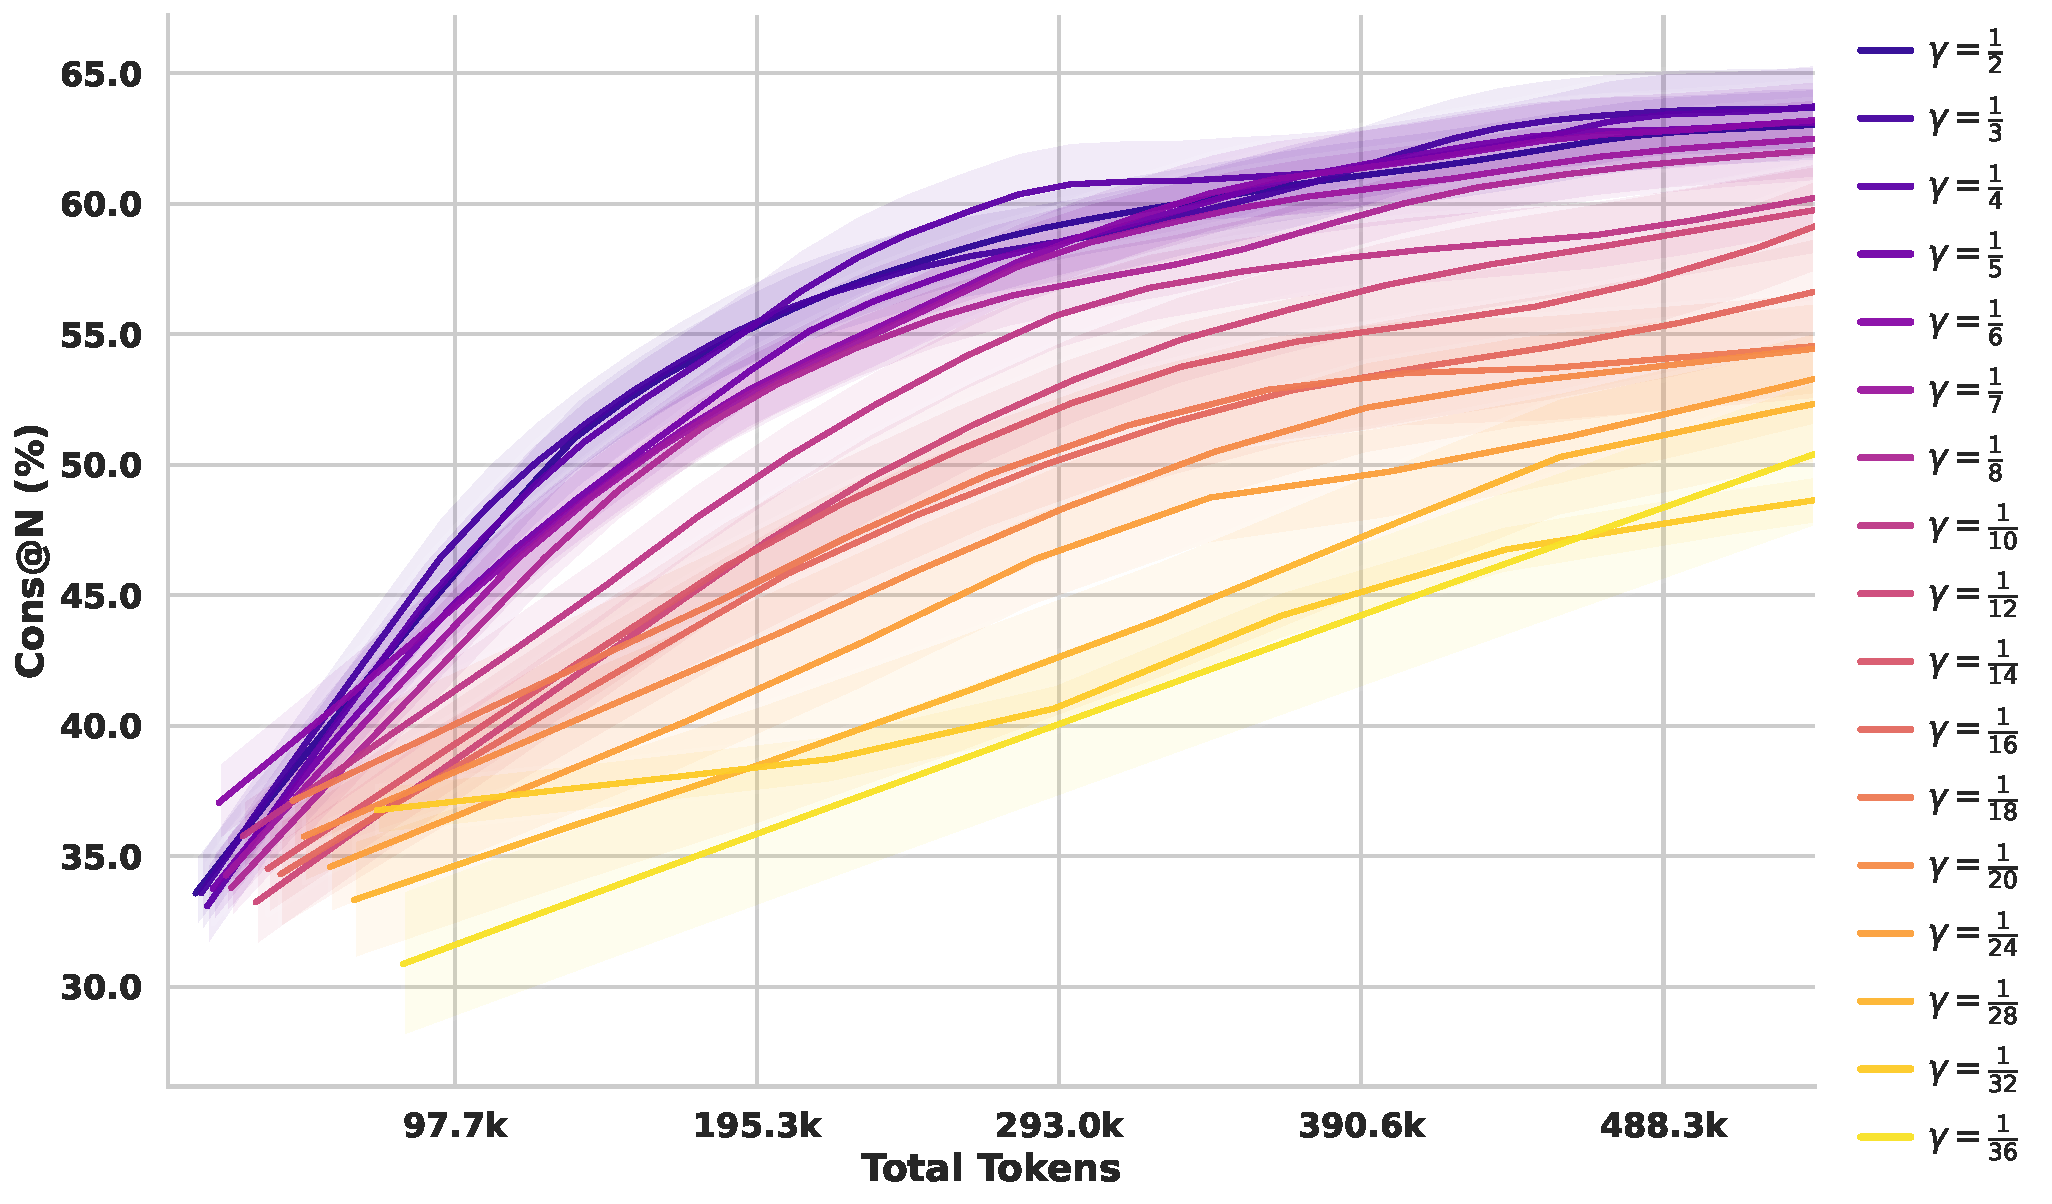
\includegraphics[height=5.0cm, keepaspectratio]{figures/Optimal_Pruning/1.5B_aime_2048.pdf}
%     \caption{\textbf{AIME 2024 ($L_{prefix}=2048$)}. Optimal $\gamma$ shifts to aggressive pruning as budget increases.}
%     \label{fig:fit_aime_2048}
%   \end{subfigure}
%   \hfill
%   \begin{subfigure}[b]{0.45\linewidth}
%     \centering
%     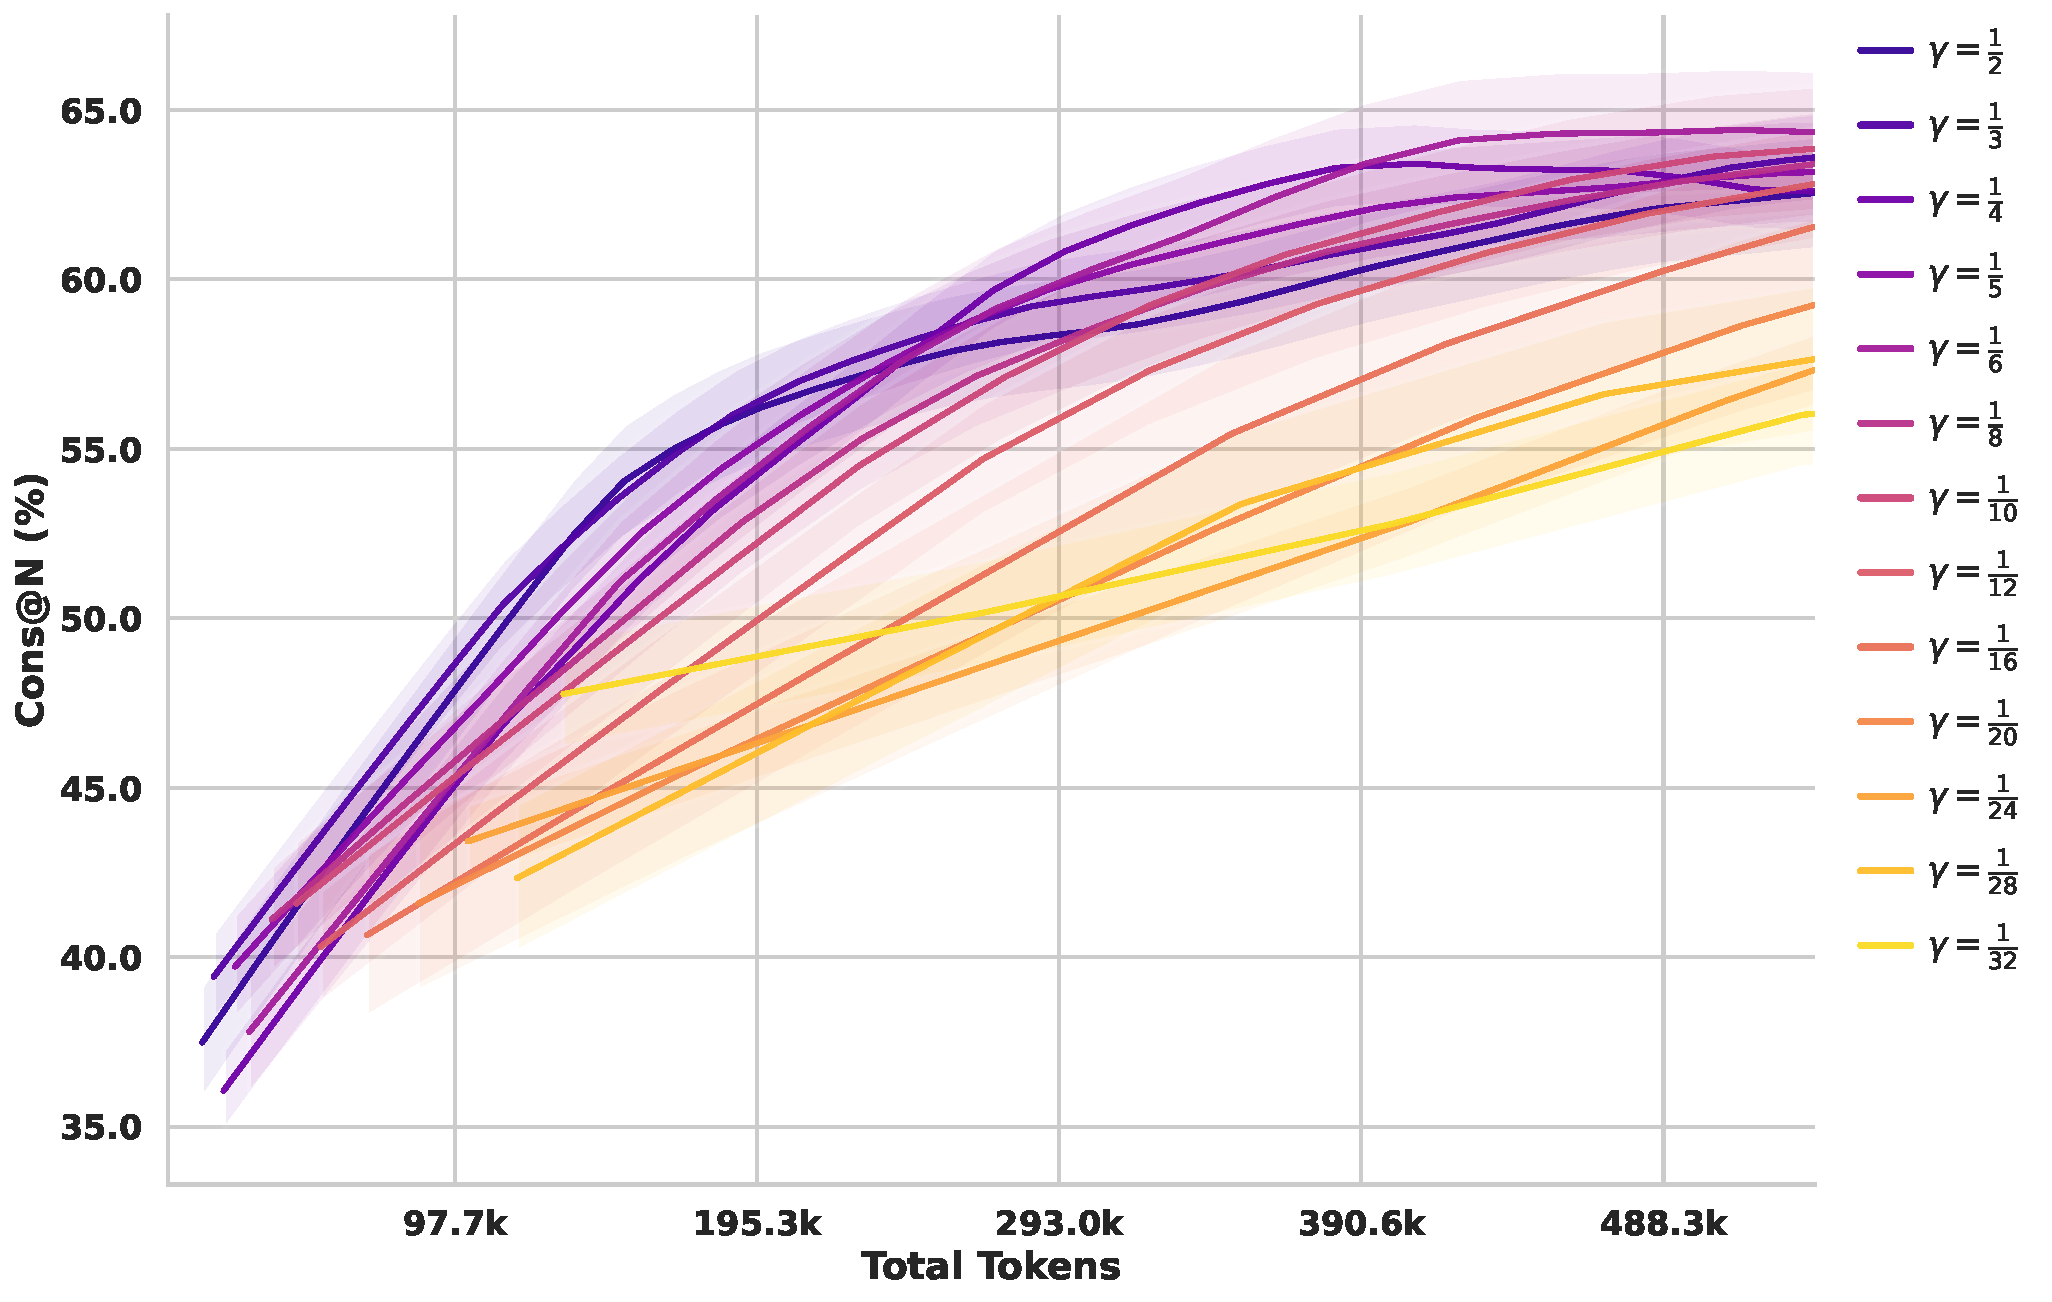
\includegraphics[height=5.0cm, keepaspectratio]{figures/Optimal_Pruning/1.5B_aime_4096.pdf} 
%     \caption{\textbf{AIME 2024 ($L_{prefix}=4096$)}. Longer context enables stable pruning at higher selectivity.}
%     \label{fig:fit_aime_4096}
%   \end{subfigure}
  
%   \vspace{1em}
  
% % --- Row 2: GPQA (Science) ---
%   \begin{subfigure}[b]{0.45\linewidth}
%     \centering
%     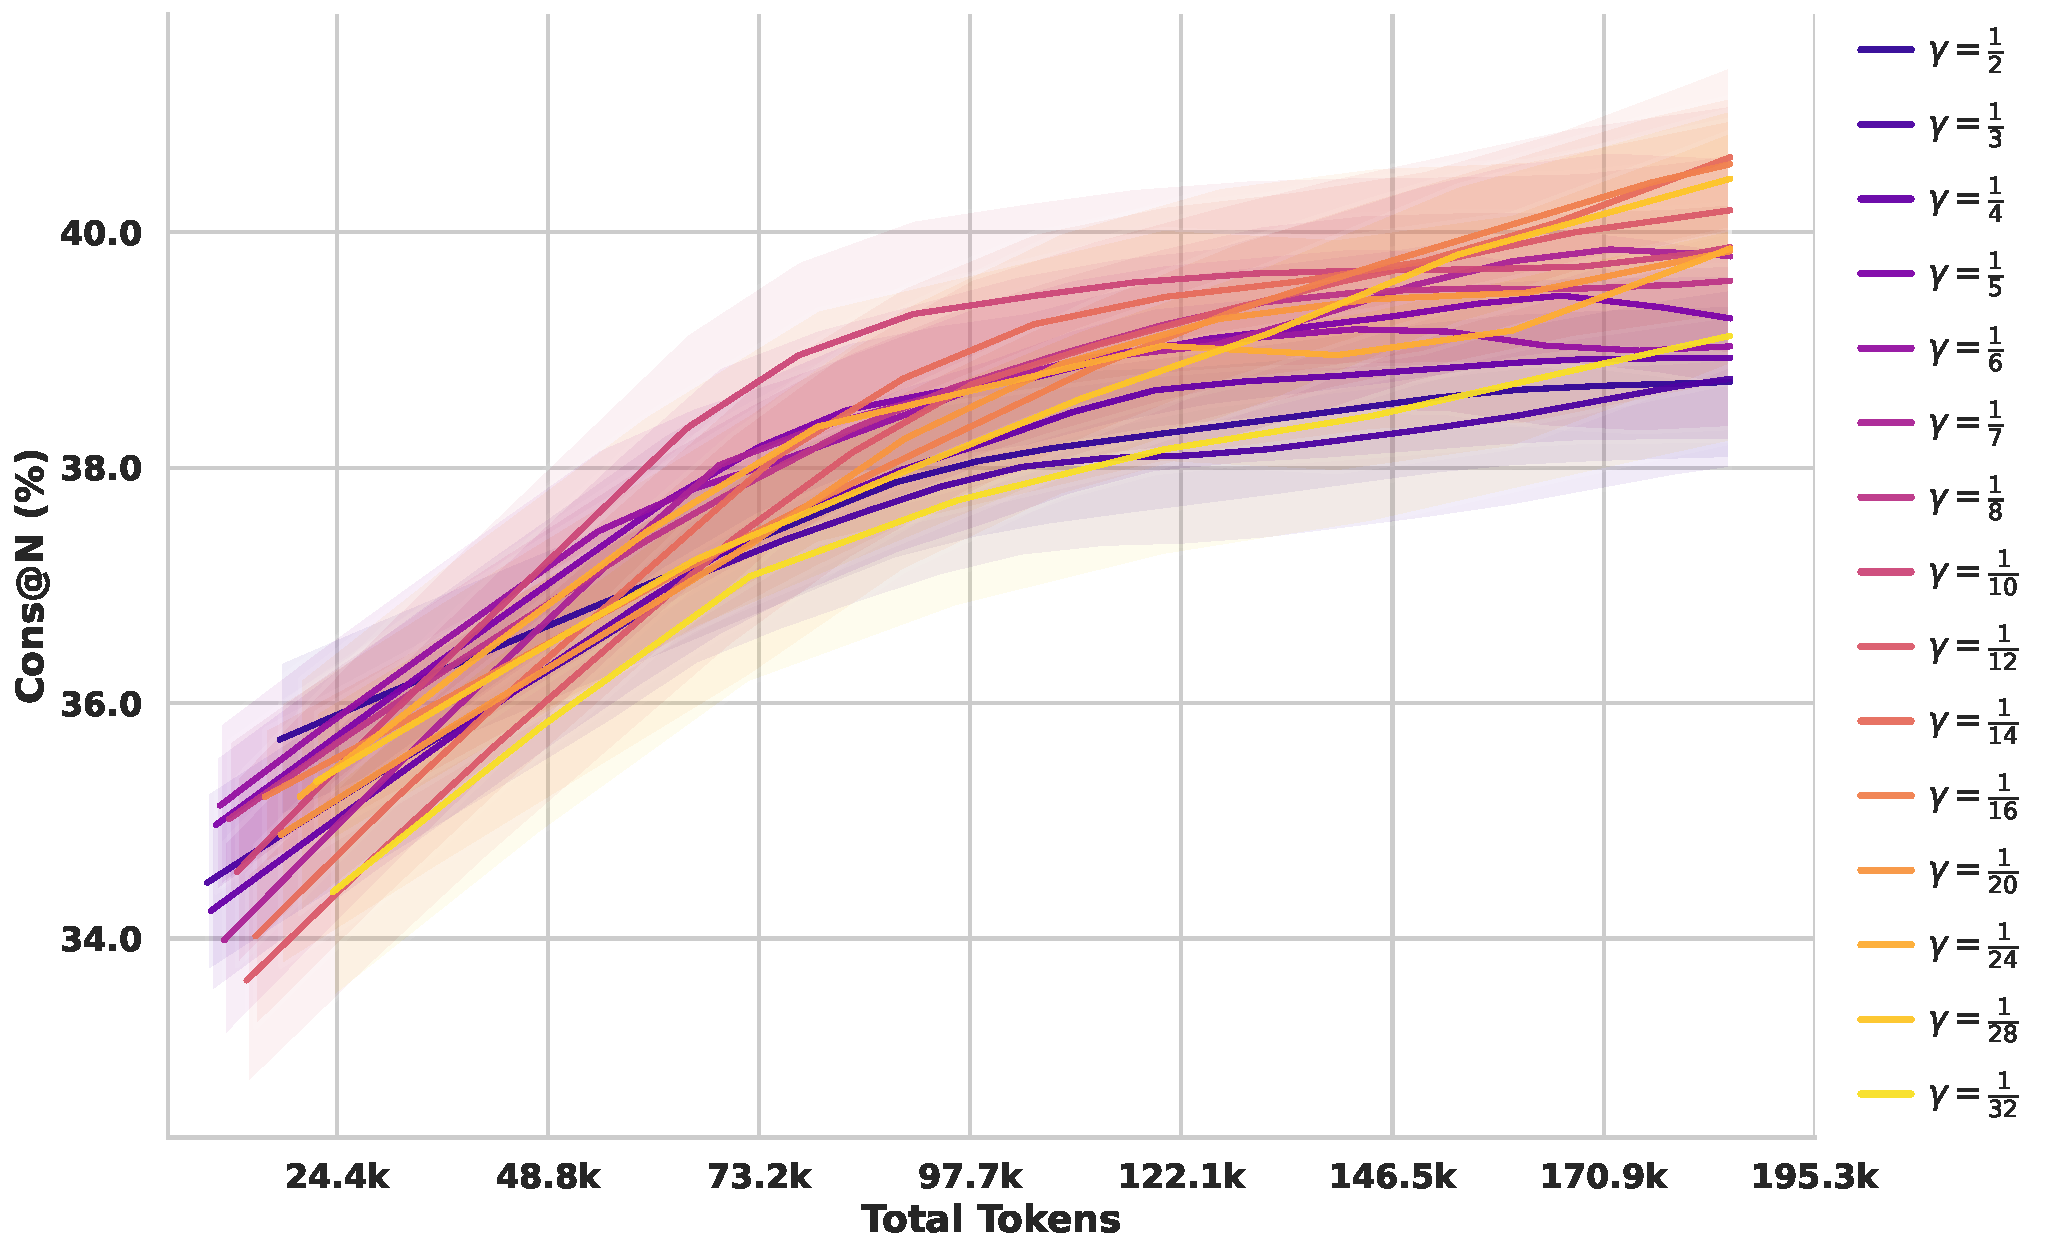
\includegraphics[height=5.0cm, keepaspectratio]{figures/Optimal_Pruning/1.5B_gpqa_512.pdf}
%     \caption{\textbf{GPQA ($L_{prefix}=512$)}. Higher compute budgets drive the optimal strategy towards more aggressive pruning.}
%     \label{fig:fit_gpqa_512}
%   \end{subfigure}
%   \hfill
%   \begin{subfigure}[b]{0.45\linewidth}
%     \centering
%     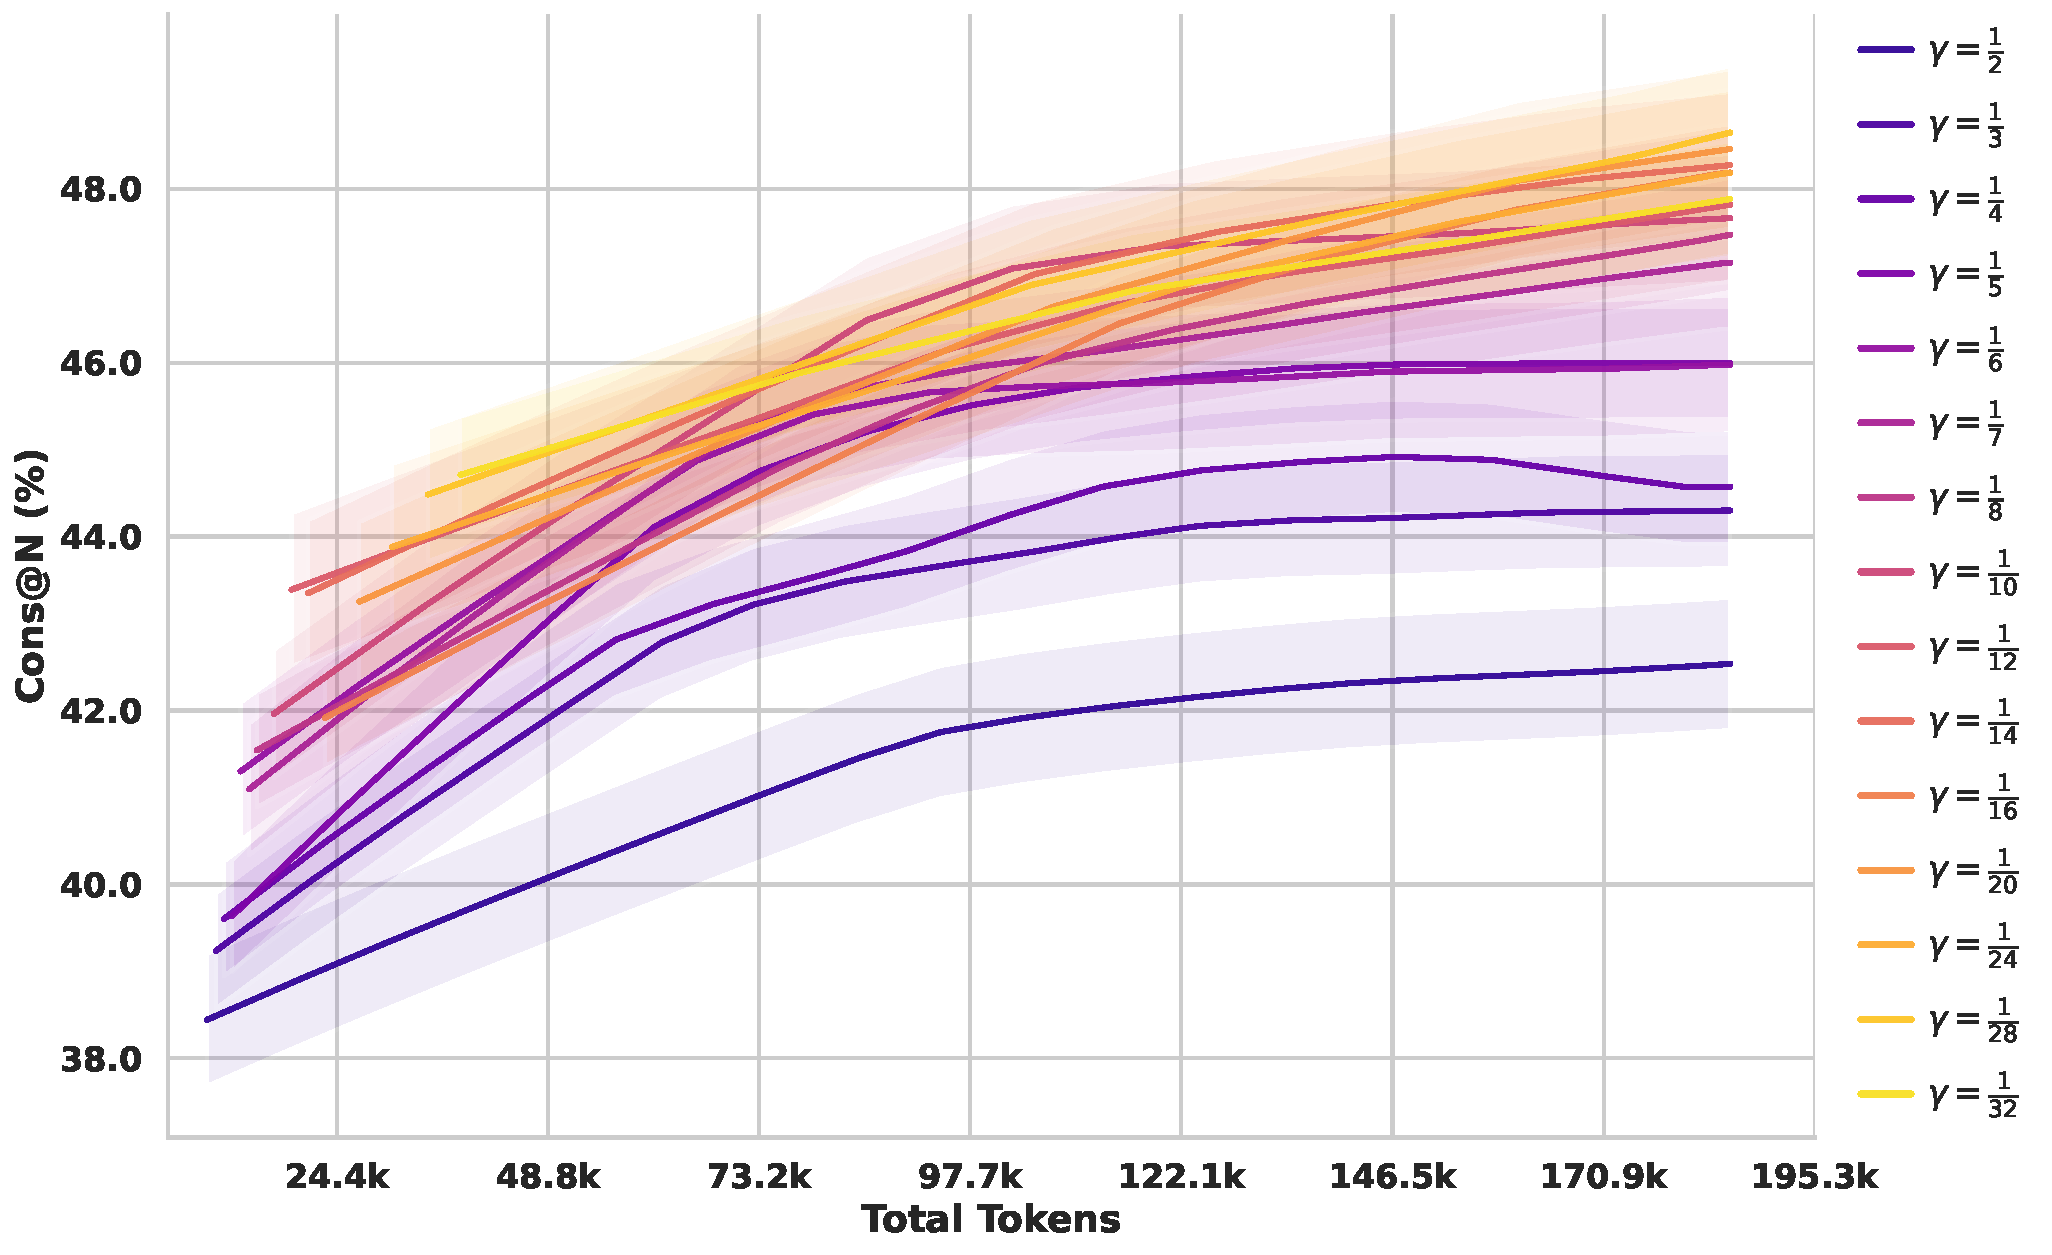
\includegraphics[height=5.0cm, keepaspectratio]{figures/Optimal_Pruning/1.5B_gpqa_1024.pdf} 
%     \caption{\textbf{GPQA ($L_{prefix}=1024$)}. This scaling behavior remains consistent even with extended context windows.}
%     \label{fig:fit_gpqa_1024}
%   \end{subfigure}
  
%   \caption{
%   \textbf{Empirical Optimization Surfaces.} 
%   We visualize the impact of varying the retention ratio $\gamma$ (represented by different curves) across increasing compute budgets. 
%   }
%   \label{fig:scaling_raw_data} 
% \end{figure*}




\section{Extended Attention Analysis}
\label{app:mechanistic_interpretability}

In Section~\ref{subsec:interpretability}, we hypothesize that the \textbf{STOP} module acts as a process-oriented evaluator. To empirically validate this, we analyze the attention patterns in Figure~\ref{fig:more_cases}.


\noindent\textbf{Universal Attention Pattern.}
Consistent with the findings in Section 5.3, \textbf{STOP} exhibits a broad attention pattern across all samples. Regardless of the score, the module consistently tracks structural discourse markers (e.g., ``Wait'', ``Hmm'', ``Therefore'', ``but'', ``\textbackslash n\textbackslash n'') as well as the final answer text. This confirms that the module monitors the structural progression of the reasoning chain.


\noindent\textbf{Distinguishing Quality via Attention Focus.}
However, a critical distinction determines the quality score.
In \textbf{High-Scoring Trajectories} (Figures~\ref{fig:more_cases}\subref{fig:viz_high_1} and \subref{fig:viz_high_2}), attention prioritizes \textbf{logical negations} (e.g., ``don't'' and ``doesn't'')—which serve as cognitive pivots—over the final answer options, indicating that \textbf{STOP} values the validity of the logical derivation.
Conversely, \textbf{Low-Scoring Trajectories} (Figures~\ref{fig:more_cases}\subref{fig:viz_low_1} and \subref{fig:viz_low_2}) exhibit a pattern of \textbf{premature closure}: attention disproportionately fixates on the \textbf{answer options themselves} (e.g., the token ``C'') while neglecting the reasoning context, serving as a robust signal for identifying guessing behavior.


\begin{figure*}[h]
  \centering
  % --- Pair 1: High vs Low ---
  \begin{subfigure}[b]{0.48\linewidth}
    \centering
    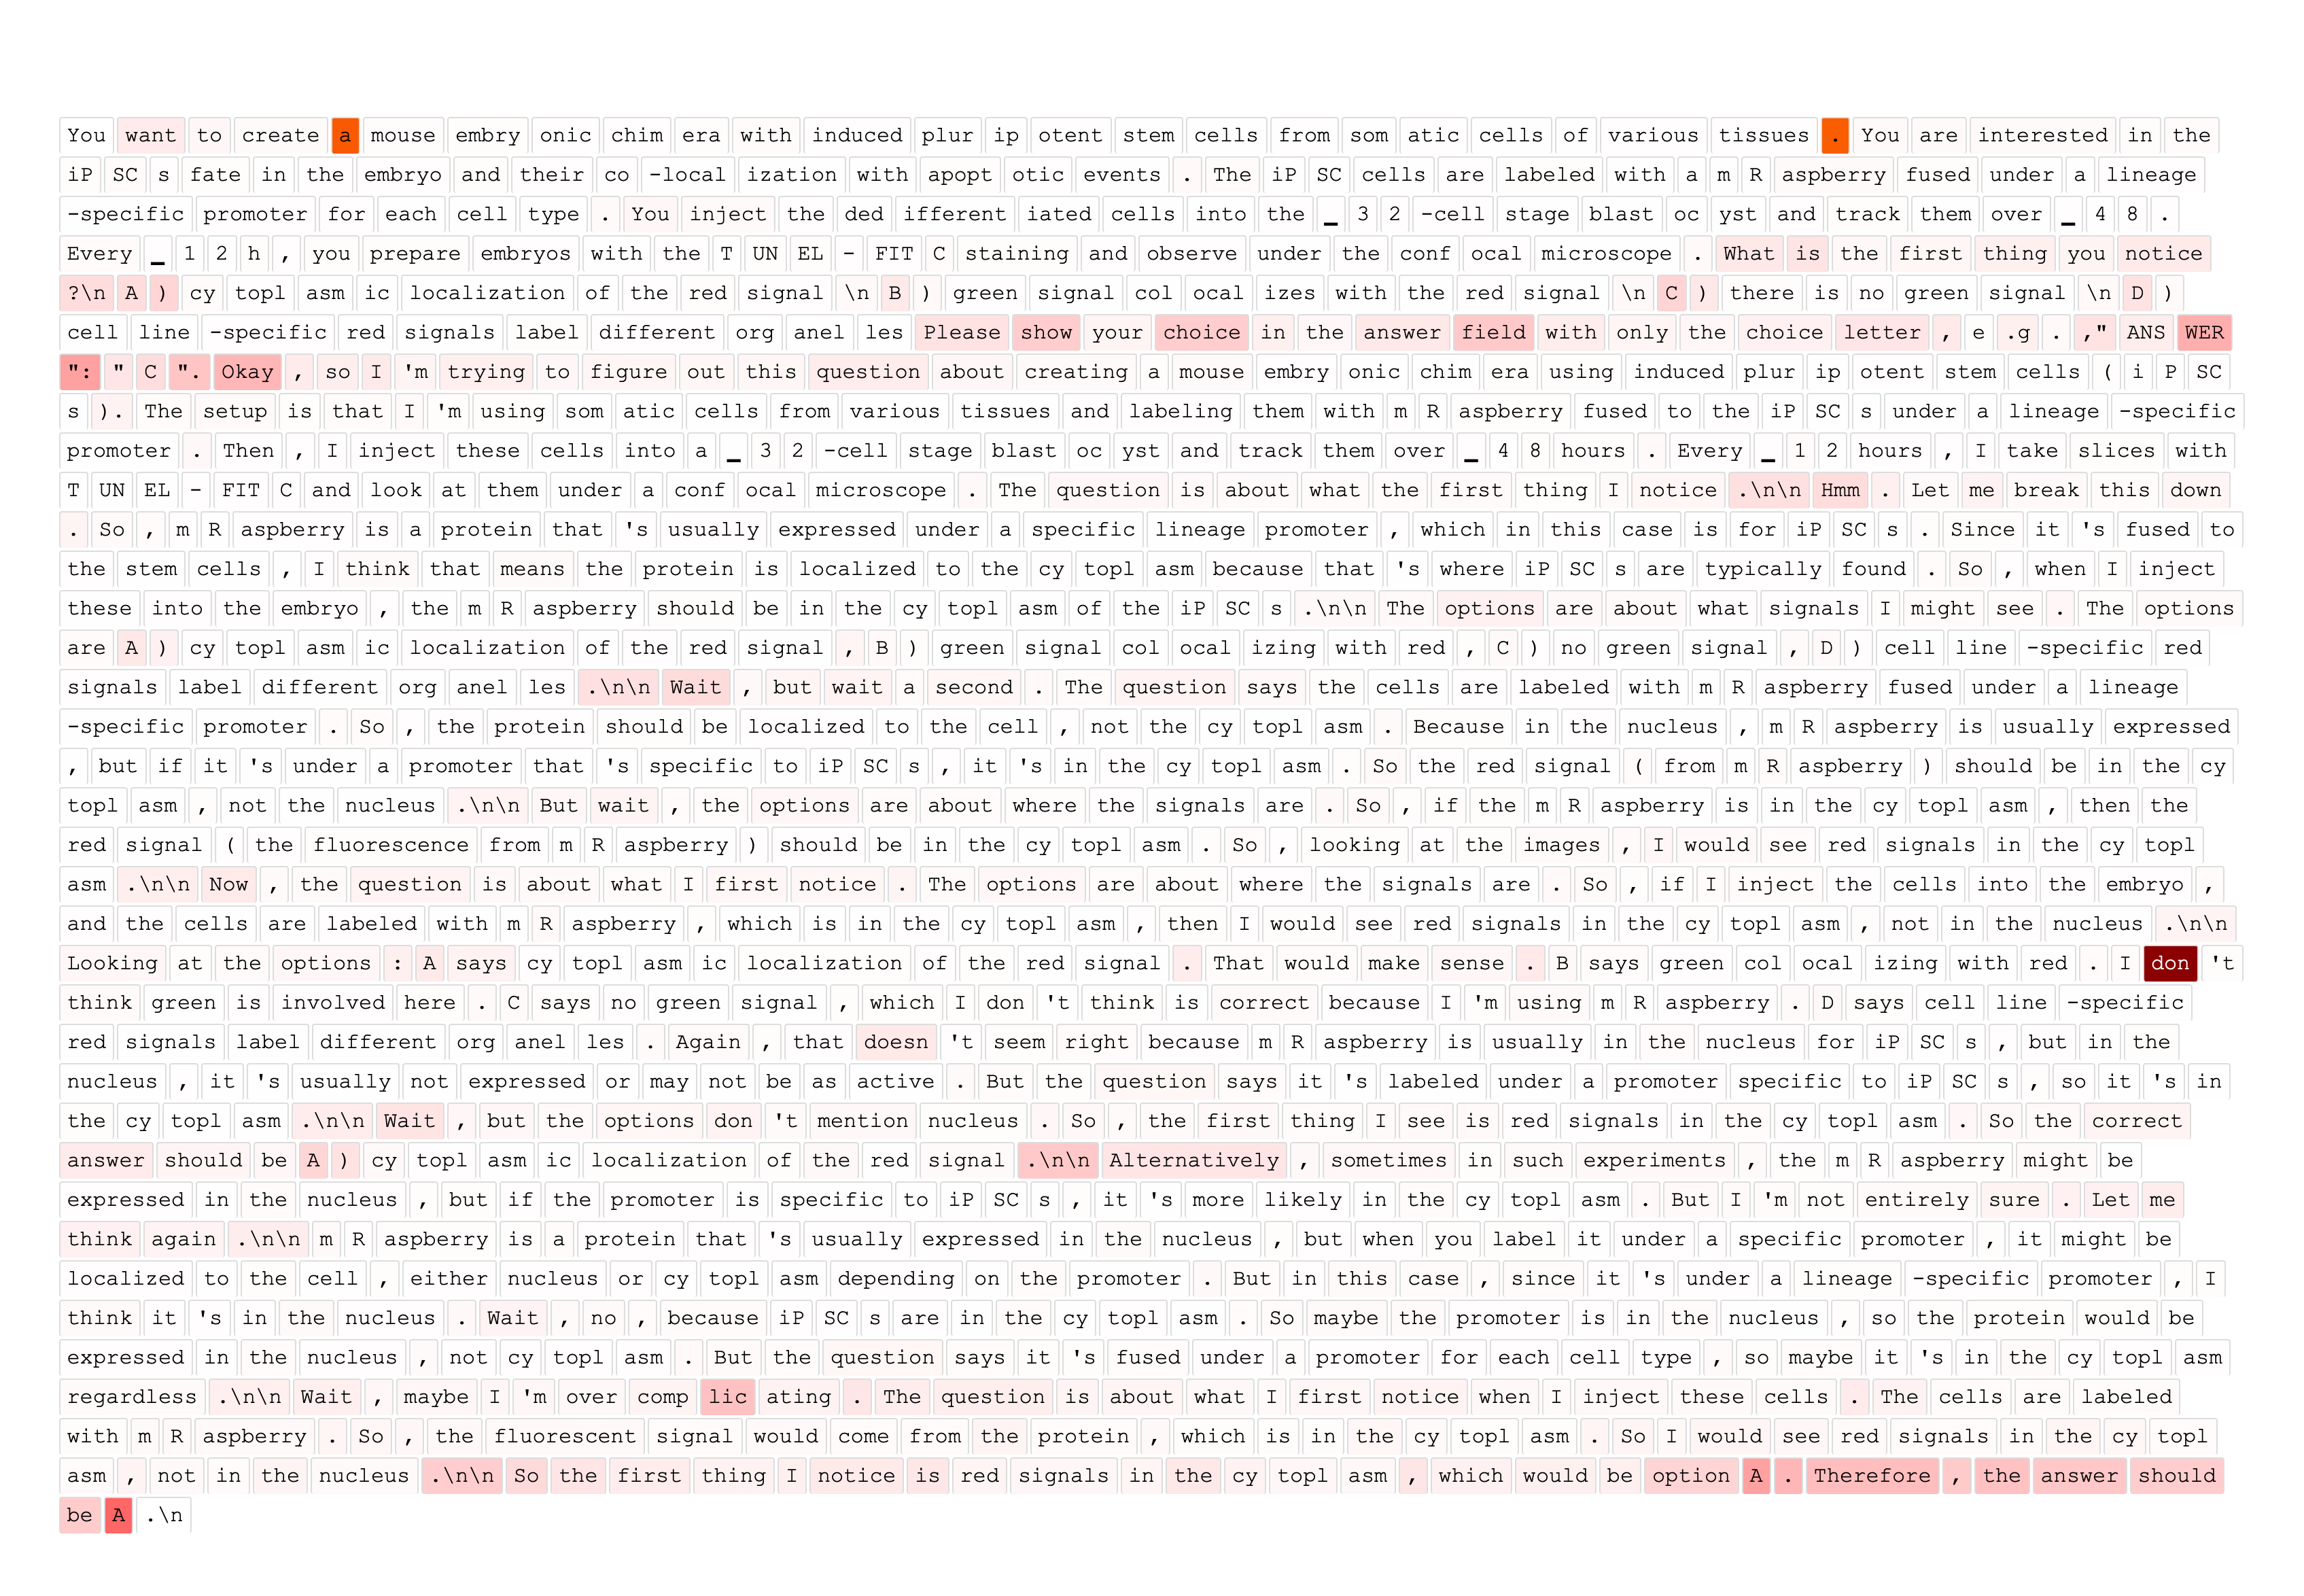
\includegraphics[height=5.0cm, keepaspectratio]{figures/high_case1.png}
    \caption{\textbf{High-scoring Case.} The module focuses on the logical negation ``don't'' (a cognitive pivot) rather than simply jumping to the answer option.}
    \label{fig:viz_high_1}
  \end{subfigure}
  \hfill
  \begin{subfigure}[b]{0.48\linewidth}
    \centering
    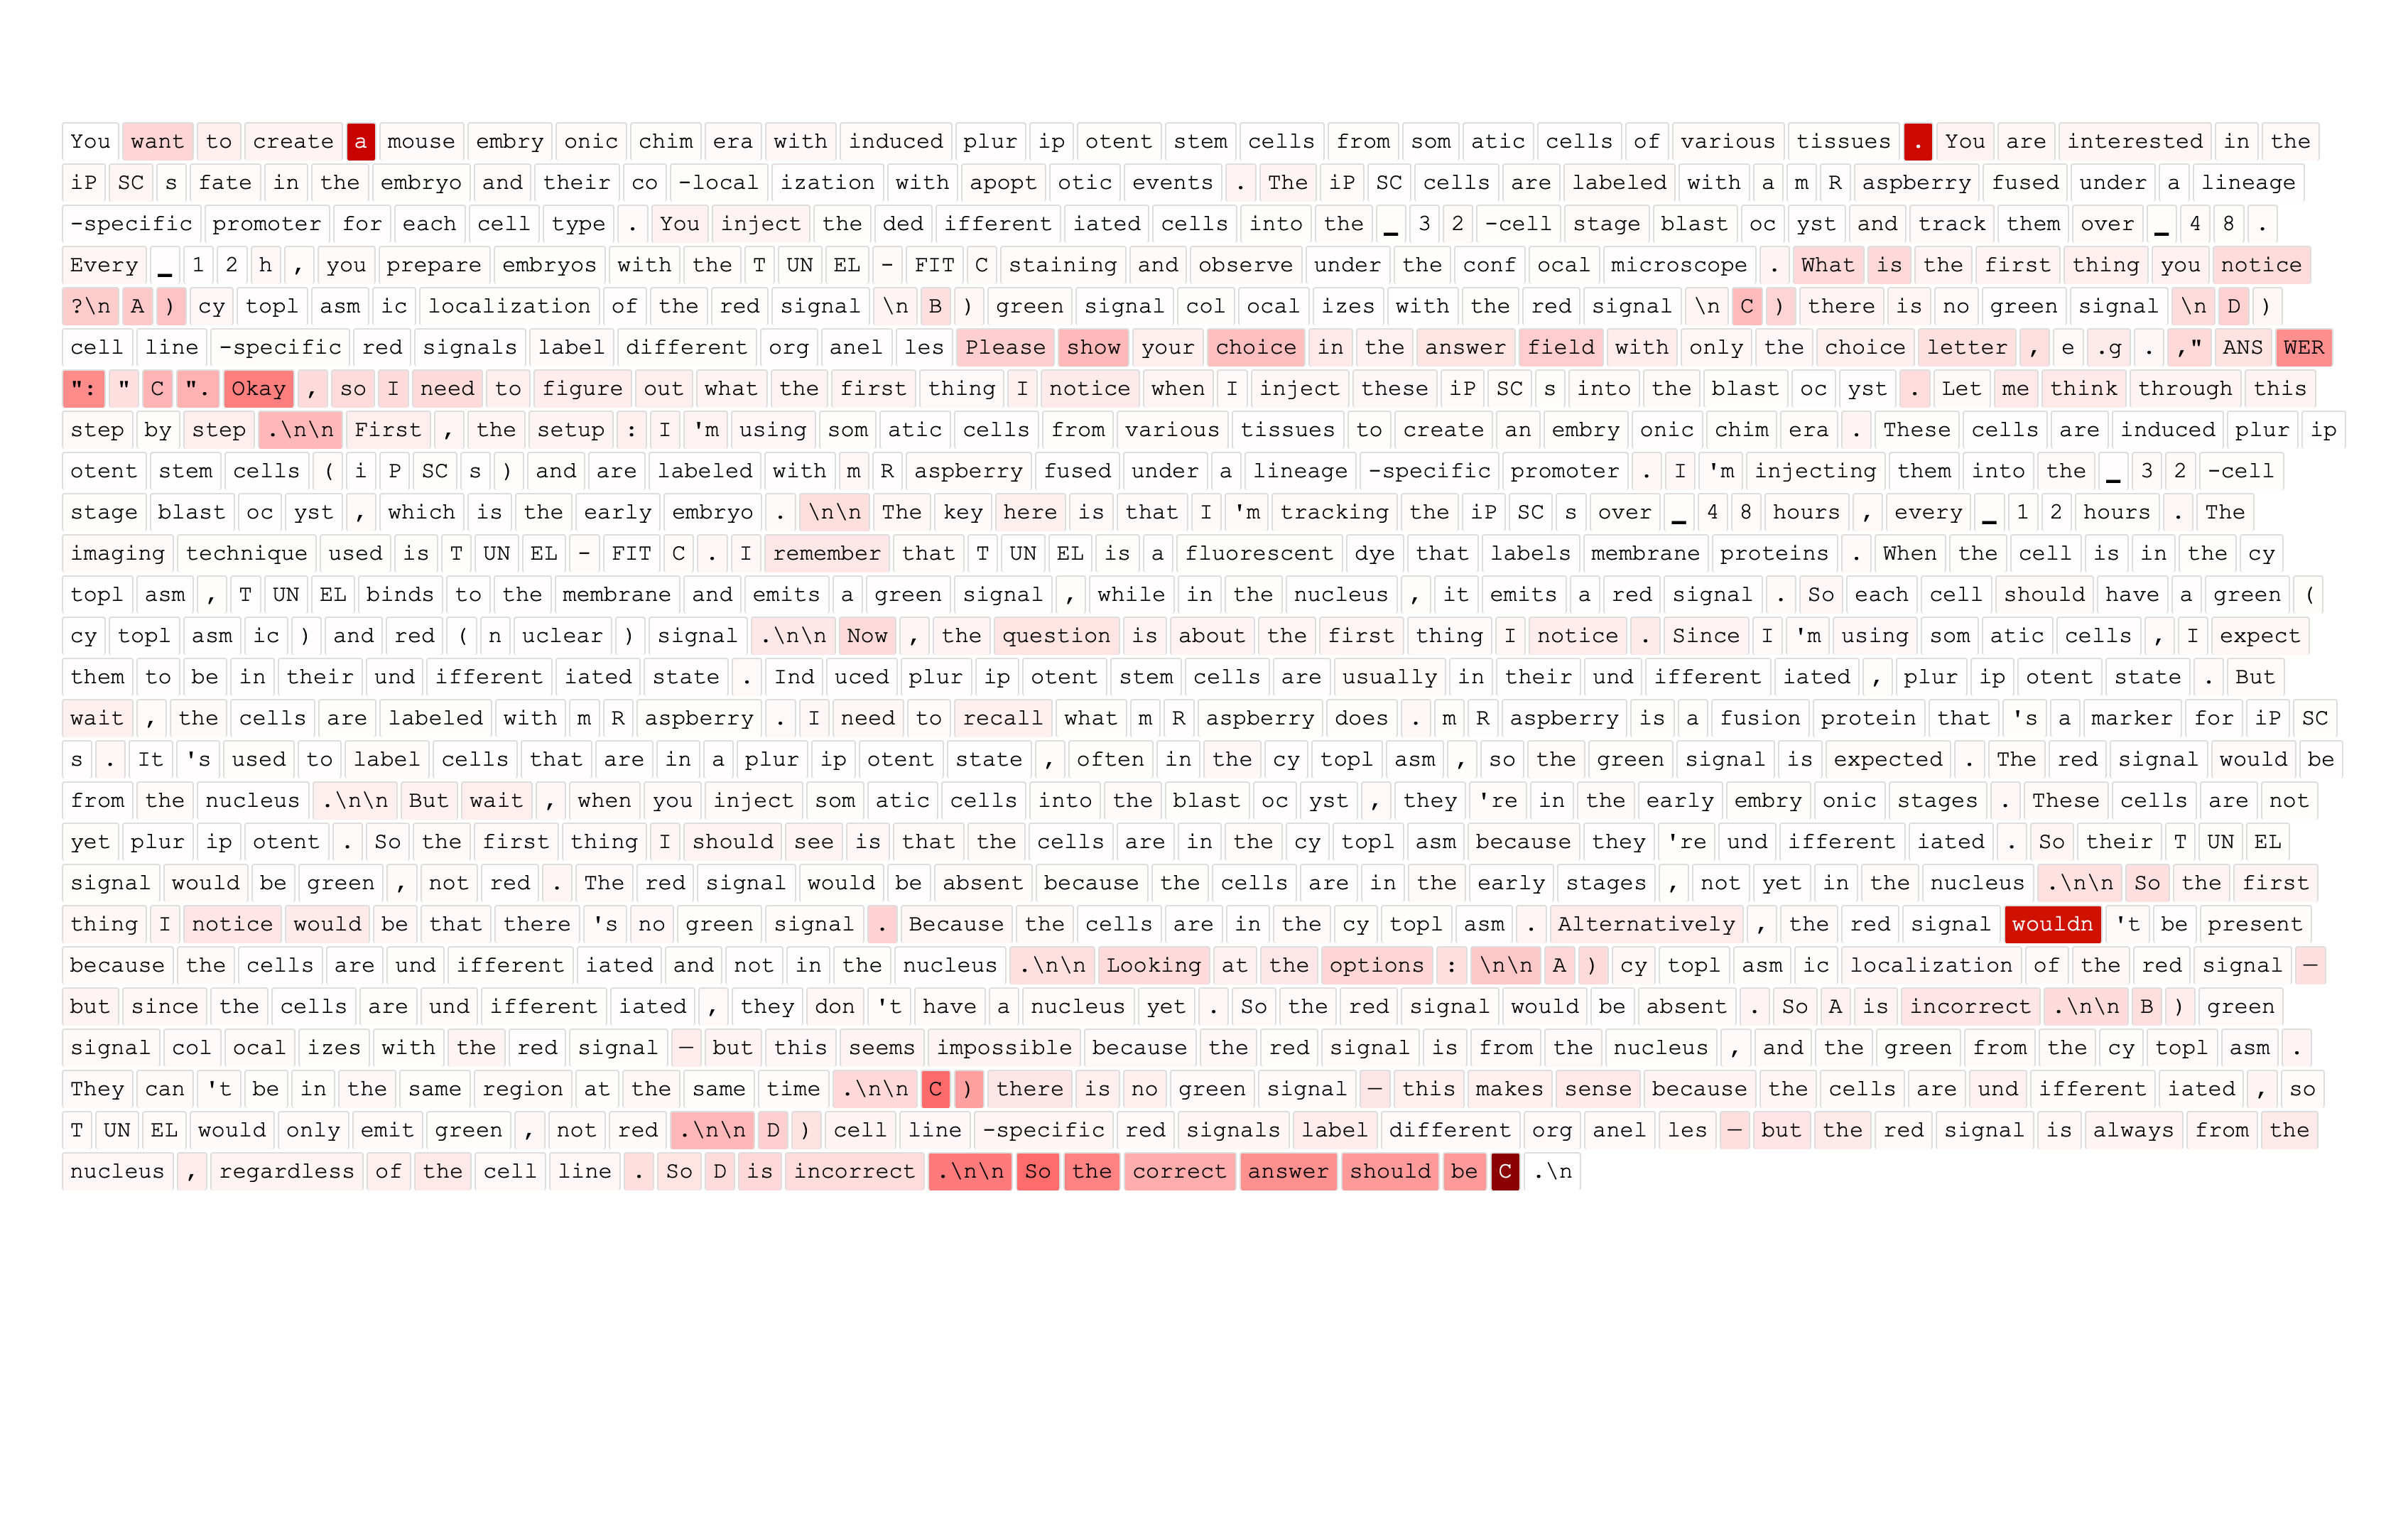
\includegraphics[height=5.0cm, keepaspectratio]{figures/low_case2.png}
    \caption{\textbf{Low-scoring Case.} Attention concentrates heavily on the answer option itself (``C''), ignoring the sparse reasoning context.}
    \label{fig:viz_low_1}
  \end{subfigure}

  \vspace{1em}

  % --- Pair 2: High vs Low ---
  \begin{subfigure}[b]{0.48\linewidth}
    \centering
    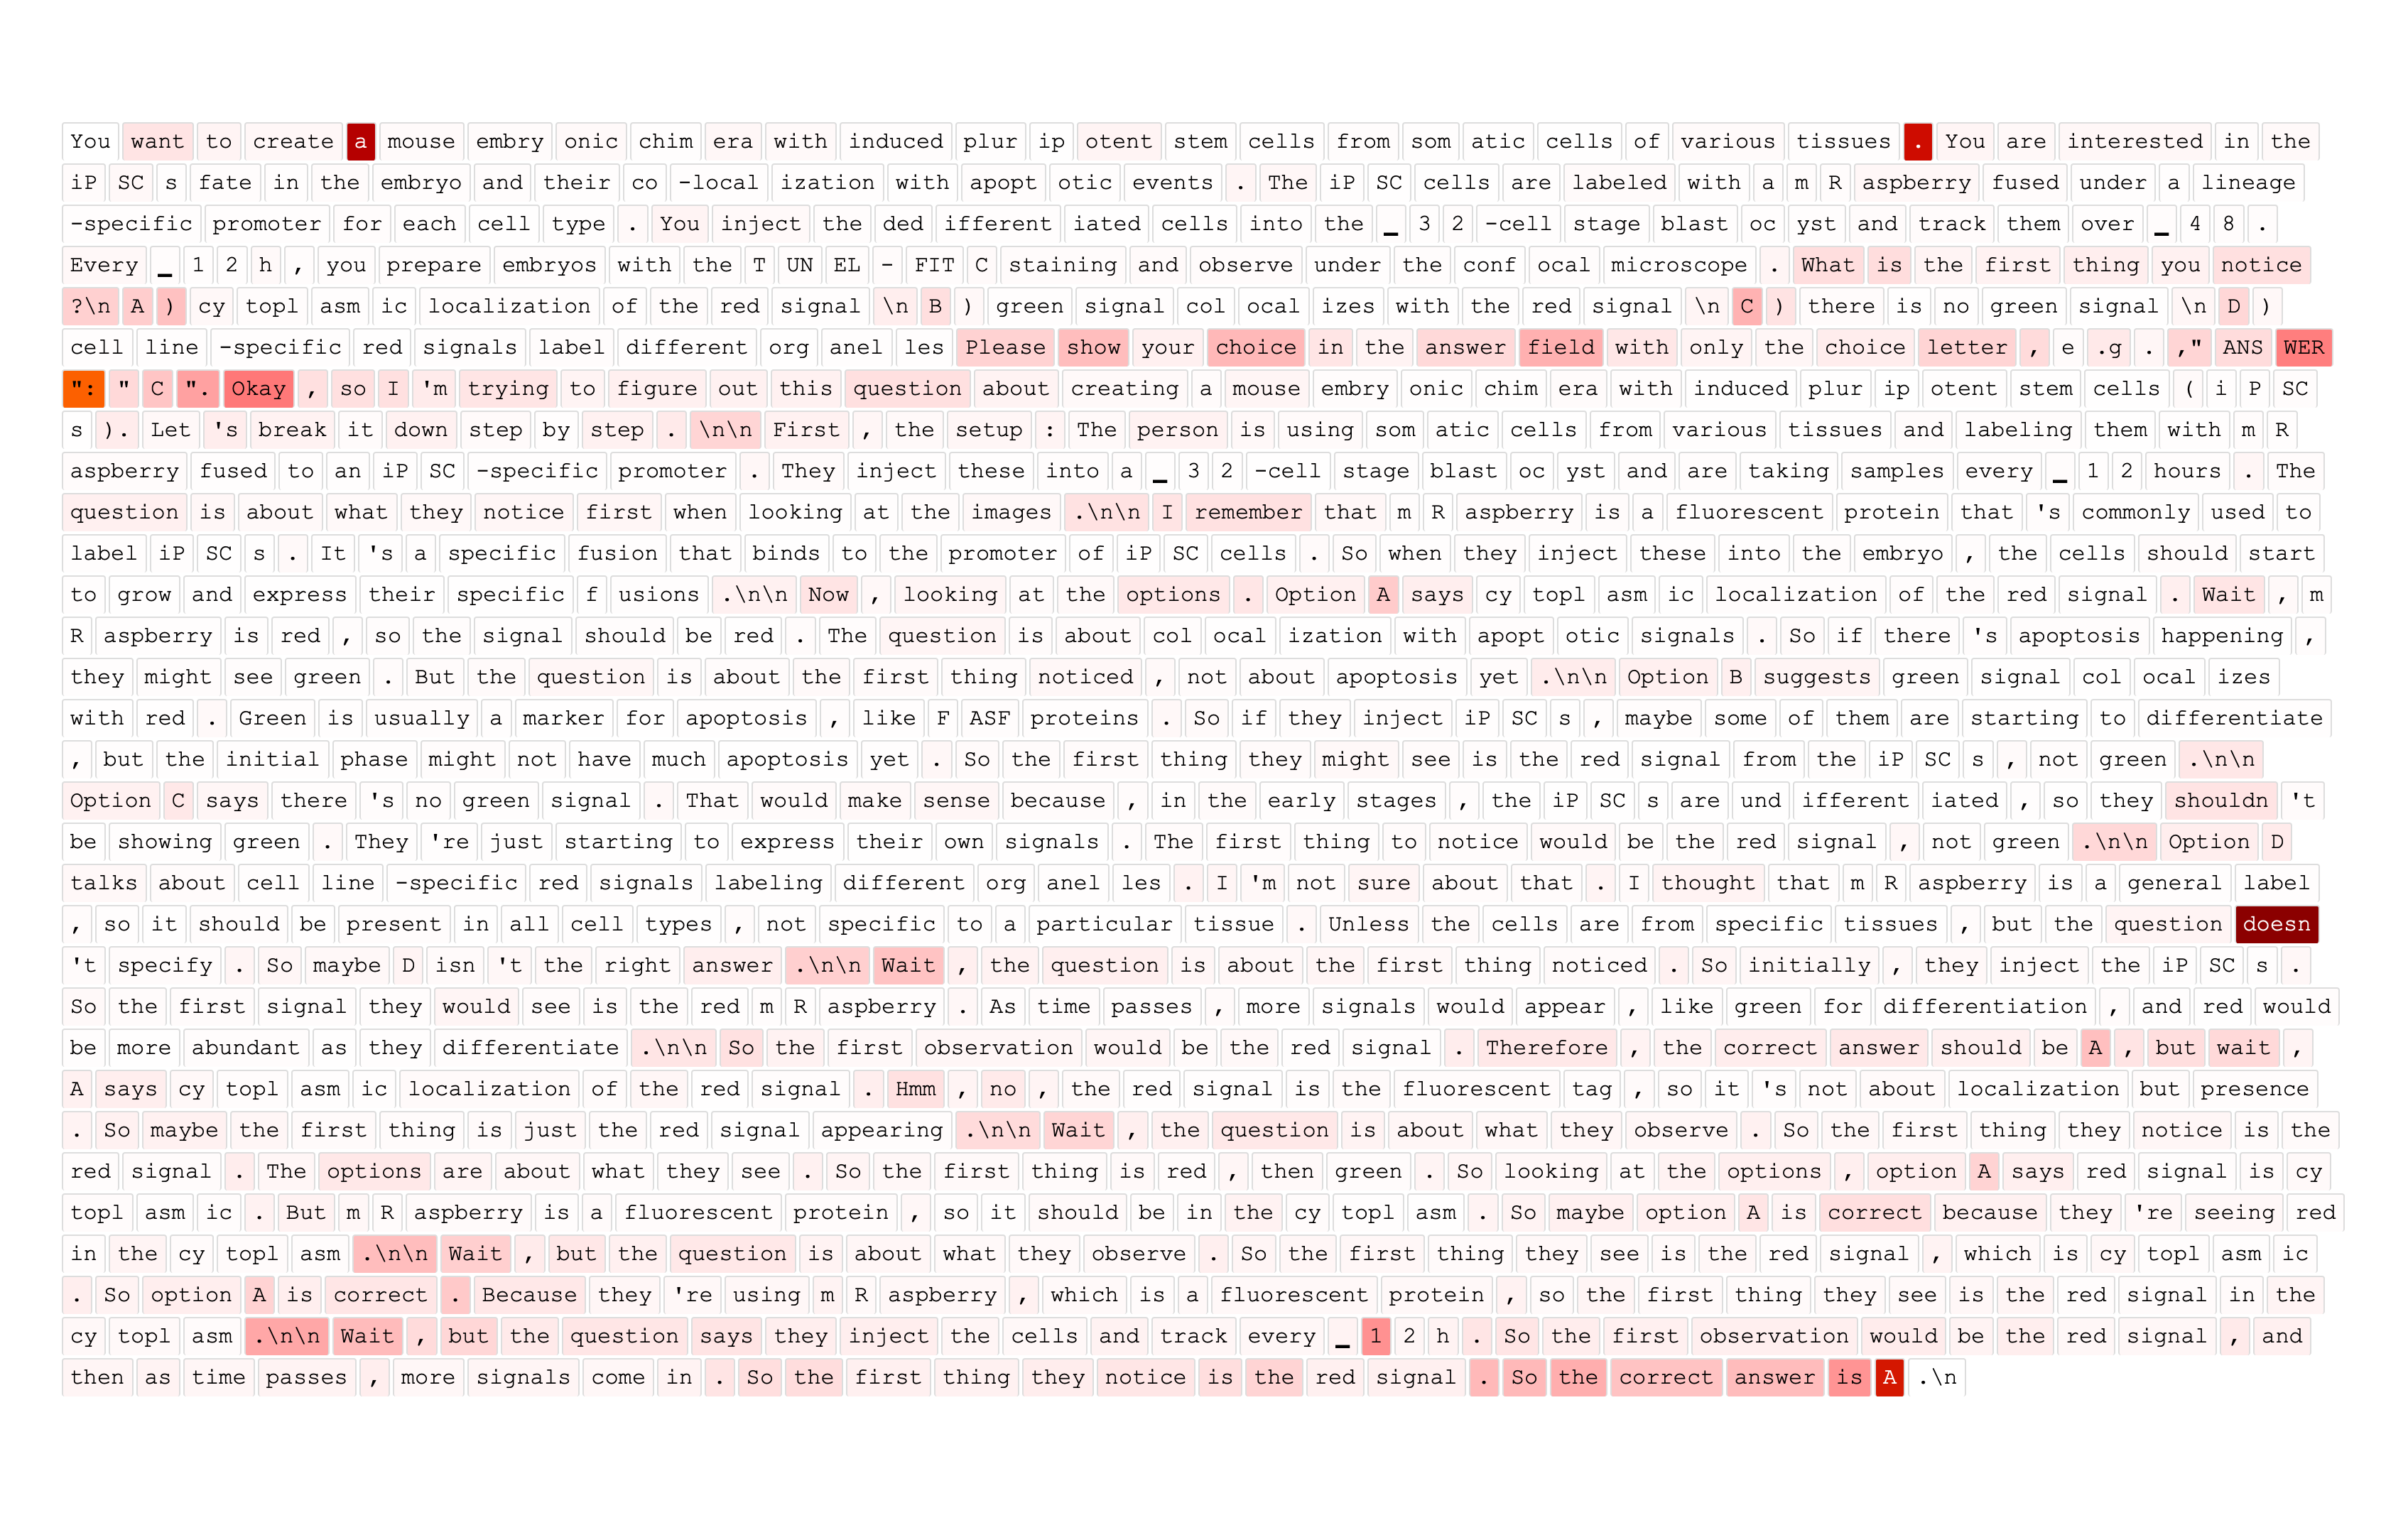
\includegraphics[height=5.0cm, keepaspectratio]{figures/high_case2.png}
    \caption{\textbf{High-scoring Case.} Similar to (a), the module attends to the logical marker ``doesn't,'' prioritizing the validity of the reasoning process over the final outcome.}
    \label{fig:viz_high_2}
  \end{subfigure}
  \hfill
  \begin{subfigure}[b]{0.48\linewidth}
    \centering
    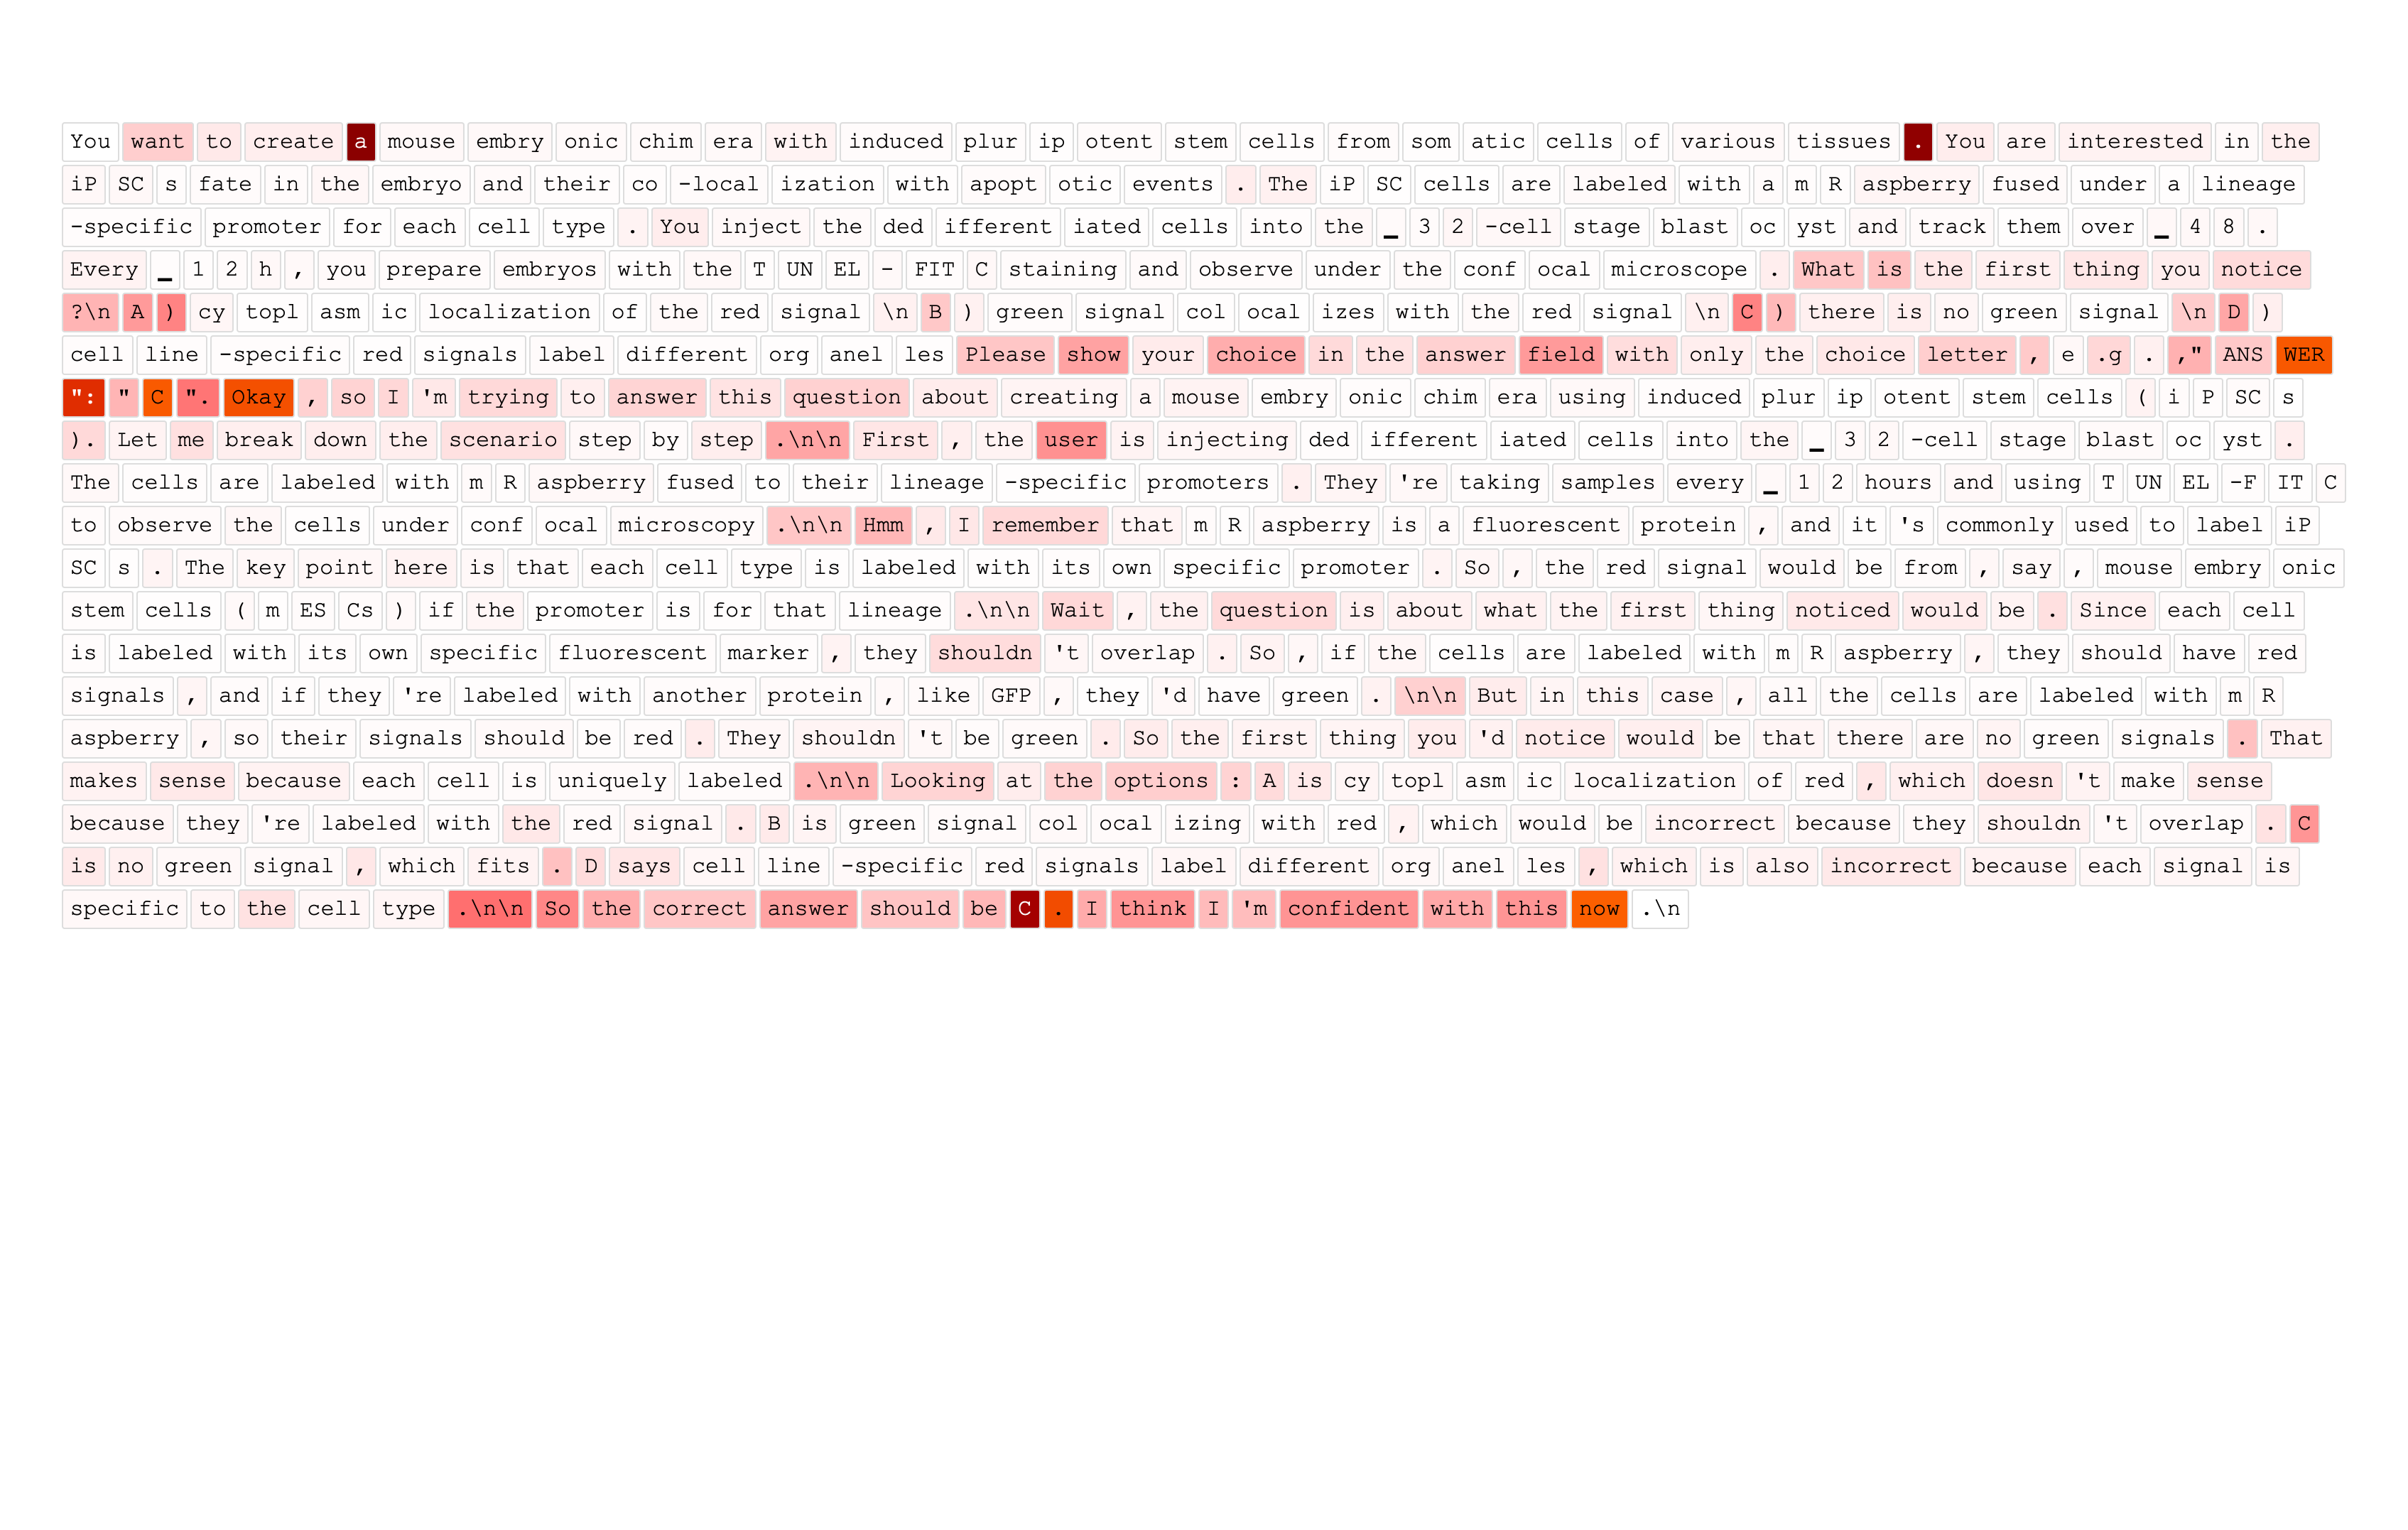
\includegraphics[height=5.0cm, keepaspectratio]{figures/low_case4.png}
    \caption{\textbf{Low-scoring Case.} The module demonstrates premature closure by fixating on the terminal choice (``C'') while bypassing critical logical intermediates.}
    \label{fig:viz_low_2}
  \end{subfigure}

  \caption{
  \textbf{Extended Visualization of \texttt{[STOP]} Attention Maps.}
  While \textbf{STOP} broadly tracks structural markers (e.g., ``Wait'', ``Therefore'') in all cases, it distinguishes reasoning quality by focus: \textbf{High-scoring paths} (left) prioritize logical pivots (e.g., ``don't''), whereas \textbf{Low-scoring paths} (right) exhibit \textbf{premature closure} by fixating on the terminal answer options.
  }
  \label{fig:more_cases}
\end{figure*}






\end{document}



